%  source("c:/data/ramadan/DataSubmitted/program/path.R"); library(knitr); library(data.table); setwd(pathprogram); knit("DIDReplication.rnw", "DIDReplication.tex"); system("platex DIDReplication"); system("pbibtex DIDReplication"); system("dvipdfmx DIDReplication")

% : cannot coerce type 'closure' to vector of type 'character': This error shows up 
% when nonexisting column name was specified in 
% Enr.Agewise[grepl("zEm.1999", sample) & grepl("wise", AgeGrouping) & grepl("1", agHH) & 
%  Age>=8 & Age<=18 & survey == 1, rate] 
% When an error ``zEm1'' not found happens, check all estimation is OK to produce \textsf{FD\_sameN\_results.rds} and the chunk \textsf{main sample size check} does not produce null results.
% zmobj2 <- c("zEm", "zSm"); zpobj2 <- c("zEp2", "zSp2", "zEp9", "zSp9")


\input{c:/migrate/R/knitrPreamble/knitr_preamble.rnw}

\usepackage{url}
\renewcommand\Routcolor{\color{gray30}}
\makeatletter
\g@addto@macro{\UrlBreaks}{\UrlOrds}
\newcommand\gobblepars{%
    \@ifnextchar\par%
        {\expandafter\gobblepars\@gobble}%
        {}}
\makeatother
\setlength{\topmargin}{-.5in}
\setlength{\oddsidemargin}{-10pt}
\setlength{\evensidemargin}{-10pt}
\setlength{\textheight}{.875\paperheight}
\setlength{\textwidth}{.8\paperwidth}
\setlength{\baselineskip}{15pt}
\setlength{\footskip}{-10pt}
\setlength{\parindent}{0pt}
\AtBeginDvi{\special{pdf:tounicode 90ms-RKSJ-UCS2}}
\special{papersize= 209.9mm, 297.04mm}
\renewcommand{\labelenumii}{\theenumii.}
\def\pgfsysdriver{pgfsys-dvipdfm.def}
\usepackage{tikz}
\usetikzlibrary{calc, arrows, decorations, decorations.pathreplacing, backgrounds}
\usepackage{adjustbox}
\usepackage[linesnumbered, ruled, lined]{algorithm2e}
\normalem % disable auto underline

\tikzstyle{toprow} =
[
top color = gray!20, bottom color = gray!50, thick
]
\tikzstyle{maintable} =
[
top color = blue!1, bottom color = blue!10, draw = white
%top color = green!1, bottom color = green!20, draw = white
]
\tikzset{
%Define standard arrow tip
>=stealth',
%Define style for different line styles
help lines/.style={dashed, thick},
axis/.style={<->},
important line/.style={thick},
connection/.style={thick, dotted},
}

\begin{document}
\setlength{\baselineskip}{12pt}

\hfil Estimation for JHR revision and resubmission\\
\hfil\MonthDY\\
\hfil{\footnotesize\currenttime}\\
\hfil Seiro Ito

\tableofcontents 

\setlength{\baselineskip}{12pt}




\begin{Schunk}
\begin{Sinput}
# below gives substitution table sbt
source(paste0(pathprogram, "substitution_table.R"))
# agHH defs, minAge, maxAge
source(paste0(pathprogram, "DefinitionsAndParameters.R")) 
dropunbalanced <- function(Z, idcol = "uniquid", returnDT = F) {
#	drop unbalanced obs (fast operation using data.table)
  require(data.table)
  dZ <- data.table(Z)
  setkeyv(dZ, idcol)
  dZ[, period := .N, by = idcol]
  # keep only individuals with largest round numbers
  dZ <- dZ[period == max(period), ]
  dZ <- dZ[, period := NULL]
  if (returnDT) dZ else data.frame(dZ)
}
source(paste0(pathprogram, "tabulate_est.R"))
source(paste0(pathprogram, "EstimatorFunctions.R"))
#source("c:/seiro/settings/Rsetting/functions.R")
\end{Sinput}
\end{Schunk}


\begin{Schunk}
\begin{Sinput}
memocovariates <- "Time variant covariates: \\textsf{yield} is Thana level paddy yield. \\textsf{program} is an indicator variable for a various school program recipient. \\textsf{mean high temperature} is mean annual temperature of the daily high, \\textsf{mean low temperature} is mean annual temperature of the daily low. \\textsf{mean rainfall} is mean annual rainfall of daily rainfall. All weather covariates are measured at Thana level. Time invariant are all measured in 1999 and are interacted with year 2002: \\textsf{agricultural household} is an indicator variable if a member in a household's primary income is agriculture (agricultural work or tenancy) or occupation is agricultural work (own land, agricultural labor, tenant, other agricultural works). \\textsf{sex (female = 1)} is an indicator variable of child gender. \\textsf{head primary, head secondary, spouse primary, spouse secondary} are indicator variables for the respective highest educational achievement. \\textsf{head sex (female = 1)} is an indicator variable of household head's gender. \\textsf{number of older brothers/sisters} are respective number of older siblings of each child. \\textsf{per member land holding} is per member land holding of the household in acres. \\textsf{per member nonland asset} is per member nonland asset values in 1000 Takas. \\textsf{own piped water, structured toilet} are indicator variables of household ownership of each facilities. All dummy variables are demeaned." 
memocovariatesForDestat <- "\\textsf{Enrolled} is an indicator variable for enrollment at school. \\textsf{Mean high temperature} is mean annual temperature of the daily high, \\textsf{Mean low temperature} is mean annual temperature of the daily low. \\textsf{Mean rainfall} is mean annual rainfall of daily rainfall. All weather covariates are measured at Thana level. \\textsf{Yield} is Thana level paddy yield. \\textsf{Program} is an indicator variable for household's program enrollment for any of antipoverty, school support programs. \\textsf{Age} is age of child in 1999.  \\textsf{Sex (female = 1)} is an indicator variable of child's gender. \\textsf{Head primary, Head secondary, Spouse primary, Spouse secondary} are indicator variables for the respective highest educational attainment. \\textsf{Head sex (female = 1)} is an indicator variable of household head's gender. \\textsf{Number of older brothers/sisters} are respective number of older siblings of each child. \\textsf{Per member land holding} is per member land holding of the household in decimal. \\textsf{Per member nonland asset} is per member nonland asset values in 1000 Takas. \\textsf{Own piped water, Structured toilet} are indicator variables of household ownership of each facilities. \\textsf{Non-Muslim} is an indicator variable for households with heads who do not identify oneself as a Muslim. \\textsf{Flood} is an indicator variable of thanas with reported flood, Aailjhar,  Chokoria, Kalia, Nilphamary Sadar, Mohadebpur. "
memo3 <- "$t$ tests compare means. For binary variables, $\\chi^{2}$ tests assess the difference in proportions, binomial tests are Fisher's exact tests that examine if the proportion in regression data is equal to the proportion in original data."
memo4 <- "Number of sample is cross sectional units per survey round. "
\end{Sinput}
\end{Schunk}

\begin{enumerate}
\vspace{1.0ex}\setlength{\itemsep}{1.0ex}\setlength{\baselineskip}{12pt}
\item	Run \textsf{CreateVariablesIn2RoundPanel.rnw} to create 1999-2002 panel. Run \textsf{Construct3RoundPanelMetAssoc.rnw} to merge with 2006 and production/weather. Then run this file. 
	\begin{itemize}
	\vspace{1.0ex}\setlength{\itemsep}{1.0ex}\setlength{\baselineskip}{12pt}
	\item	\textsf{CreateVariablesIn2RoundPanel.rnw}: Key variables and dummy interactions are created.
	\item	\textsf{Construct3RoundPanelMetAssoc.rnw}: Merged with rd 3 data and weather/production data.
	\end{itemize}
\item	If need to redefine age range, do it in Construct3RoundPanelMetAssoc.rnw, then redefine in this file and run this file.
%\item	 When an error ``zEm1'' not found happens, check all estimation is OK to produce \textsf{FD\_sameN\_results.rds} and the chunk \textsf{main sample size check} does not produce null results.
\end{enumerate}
Use 2002-1999 differences. Keep only one data set per estimation, so number of observation is determined by the most demanding specification that has least number of observations. Ages: 10 - 18.
\begin{dinglist}{43}
\vspace{1.0ex}\setlength{\itemsep}{1.0ex}\setlength{\baselineskip}{12pt}
\item	\textsf{DID1} takes a first difference by using \textsf{diff}, which computes x[t, ] - x[t-1, ], to eliminate fixed effects. Returns level and differenced data sets for each specifications.
\item	\textsf{DID2} takes a first difference data set. 
\item	We expect the Ramadan school holiday impacts to be positive for the agricultural households in 1999, or $b_{3}>0$ with $t=1999, 2002$. 
\[
\begin{aligned}
y_{t}&=b_{0}+b_{1}I[t=1999]+b_{2}I[D=1]+b_{3}I[t=1999]I[D=1]+e_{t},\\
\Delta y_{1999}&=y_{1999}-y_{2002}=b_{1}I[t=1999]+b_{3}I[t=1999]I[D=1]+\Delta e_{1999}.
\end{aligned}
\]
First-differencing using \textsf{DID1} is equivalent to $-\Delta y_{1999}=y_{2002}-y_{1999}=-b_{1}I[t=1999]-b_{3}I[t=1999]I[D=1]-\Delta e_{1999}$. So the estimate on $I[t=1999]I[D=1]$ is negative.
\item	To get back to $\Delta y_{1999}=y_{1999}-y_{2002}=b_{1}I[t=1999]+b_{3}I[t=1999]I[D=1]+\Delta e_{1999}$, I will just multiply $-1$ to the estimates. We use the switch \textsf{opposite.time.order = T, F}
to change the signs. If T, it is 1999-2002 differences.
\item	We take 2002 dummy as yr2 ($r_{t}$ in main text). We use t - (t-1) differencing for FD estimates. 
\end{dinglist}

\begin{description}
\vspace{1.0ex}\setlength{\itemsep}{1.0ex}\setlength{\baselineskip}{12pt}
\item[spattern]	A schooling history indicator, binary indicators for schooling in each round is pasted together, so 111 indicates always goers and 110 indicates out of school at round 3. 
\item[exist]	A survey response history indicator where we pasted the binary indicator of survery response in each period. Value of \textsf{110} is attrition at round 3, \textsf{001} indicates first observed in round 3. There is no \textsf{101} by definition because an individual will never be observed after attrition. \textsf{001} sample from 2006 data does not have school program information for 1999, 2002, so we will not use them. This leaves us with the sample of \textsf{110, 111}. 
\end{description}


% One can define a function to align comments: https://tex.stackexchange.com/a/216137
\setlength{\baselineskip}{10pt}
\begin{algorithm}
\caption{Structure of estimation procedure}
\DontPrintSemicolon
\SetAlgoNoLine
samples $\leftarrow$ c("main", "placebo")\;
\tcc{main data: (Exist \{110, 111\} or spattern $\neq$ 000) $\times$ baseline year 1999}
\tcc{placebo data: (Exist \{110, 111\} or spattern $\neq$ 000) $\times$ (baseline year 1999 [too young children] or 2002 [same age range born 3 years later])}
zmobj $\leftarrow$ c("zEm.1999", "zSm.1999") \tcc*[r]{main data sets}
zpobj $\leftarrow$ c("zEp.2002", "zSp.2002", "zEp.1999", "zSp.1999")  \tcc*[r]{placebo data sets}
agecutoff $\leftarrow$ 1:3\;
z23 $\leftarrow$ c("z2", "z3")\;
aghh.defs $\leftarrow$ c("agHH0", "isagHH", "hdagHH", "ocagHH")\;
Clustering $\leftarrow$ c("LiangZeger", "Satterthwaite", "WildClusterBoot")\;
\For( \tcc*[f]{choose main or placebo sample}){ii in 1:length(samples)}{
  zSobj $\leftarrow$ c("zmobj", "zpobj")[ii]\;
  \For(\tcc*[f]{choose data in main/placebo data sets}){jj in 1:length(zSobj)}{
     z1 $\leftarrow$ changehyphen(get(zSobj[jj]))\;
     \For(\tcc*[f]{lower age cutoff: 10 - 12}){s in agecutoff}{
        s0 $\leftarrow$ (10:12)[s]\;
        iiid $\leftarrow$ s0 $\leqslant$ AgeInYYYY $\leqslant$ 18\;
        z2 $\leftarrow$ z1[uniquid \% in\% iiid \& survey $!=$ cutout.year, ]\;
        z3 $\leftarrow$ z2[sd == 1, ] \tcc*[r]{nuclear family}
        \For(\tcc*[f]{nuclear or extended family}){j in 1:length(z23)}{
          zz0 $\leftarrow$ get(z23[j])\;
          \For(\tcc*[f]{ag HH definitions}){m in 1:length(aghh.defs)}{
            agHH $\leftarrow$ aghh.defs[m]\;
            \For(\tcc*[f]{small number of cluster correction}){cl in 1:3}{
              clustering choice $\leftarrow$ Clustering[cl]\;
	            \For(){k in 1:length(regressorsS)}{
	              do estimation with k-th set of covariates\;
	            }
            }
          }
        }
     }
   }
}

\end{algorithm}
\ULforem % enable auto underline



\begin{Schunk}
\begin{Sinput}
Usesd2 <- F
DemeanAtIndividualLevel <- F
\end{Sinput}
\end{Schunk}


\section{Sample selection}

Note that we use the balanced portion of the panel between round 1 and 2. 

\subsection{Summary}

\textsf{zFm.1999} is \textbf{\textsf{F}}ull sample, for \textbf{\textsf{m}}ain estimation to check 1999-2002 changes, with cohorts of ages 10-19 in \textbf{\textsf{1999}}. \textsf{zFm.2002} is full sample, for \textbf{\textsf{m}}ain estimation to check 1999-2002 changes, with cohorts of ages 10-18 in \textbf{\textsf{2002}}, or cohorts of ages 7-15 in \textbf{\textsf{1999}}. \textsf{zFp.2002} is full sample, for \textbf{\textsf{p}}lacebo estimation to check 2002-2006 changes, with cohorts of ages 10-18 in 2002. 
Idea on selecting sample:
\begin{description}
\vspace{1.0ex}\setlength{\itemsep}{1.0ex}\setlength{\baselineskip}{12pt}
\item[zF, fulll]	Original sample with no selection. We do not use this full sample.
\item[zE, exist $==$ \{110, 111\}]	This sample excludes the individuals who do not appear in the roster of round 1. There are two possible reasons for such individuals to appear only in the later rounds: Measurement errors in the first round and new members who joined households in later rounds. We do not consider lack of entry in the rounds 2 and 3 as measurement errors, because they appear twice which makes measurement errors unlikely. If we trust the round 1 information on roster more than the later rounds, this is the sample to use. If the members appear only in the later rounds are new members who joined households, we should not include these individuals because they were not the original household members at round 1. 
%\item[zS, spattern $!$= 000]	A glance at \textsf{spattern-age2002} tabulation shows that \textsf{spattern = 000} are of elder ages who might have finished schooling. So we can ignore \textsf{spattern = 000} with above 18 or so on schooling issues. Another reason for dropping them is they do not contribute to identification. Dropping these also drops significant portion of \textsf{exist=\{001\}}. 
\end{description}

Another layer of sample selection is direct offspring of household heads. We discard extended household portion of families because we cannot use parental covariates, and there is a chance parents outside households may be making schooling decisions.

Placebo testing of nonexisting 2002 effects:
\begin{description}
\vspace{1.0ex}\setlength{\itemsep}{1.0ex}\setlength{\baselineskip}{12pt}
\item[Same age group]	10-max year olds in 2002 (same age group, different individuals) are estimated for 2002 effects that are presumed not to exist. Larger standard errors despite larger sample size relative to main results. Point estimates are also smaller, leading to estimates with higher p values. Use subsample defined by \textsf{AgeInRangeR2==T}.
\item[Same individuals]	10-max year olds in 1999 (same individuals) are estimated for 2002 effects that are presumed not to exist. Smaller sample size and smaller point estimates relative to main results lead to not statistically significant results. Use subsample defined by \textsf{AgeInRangeR1==T}.
%\item[Younger cohorts]	8-12 year olds in 2002 who were too young (5-9 year olds) to have been exposed to hypothesised impacts in 1999 are estimated for 2002 effects that are presumed not to exist. Smaller sample size and smaller point estimates relative to main results lead to not statistically significant results.
\end{description}

Falsification testing of other mechahisms affecting enrollment rates:
\begin{description}
\vspace{1.0ex}\setlength{\itemsep}{1.0ex}\setlength{\baselineskip}{12pt}
\item[Non-muslims]	Non-muslims are least affected with Ramadan except for exam schedule changes. Including a non-muslim dummy and its interaction with an agricultural household dummy does not affect main estimates. Estimates are not statistically significant.
\item[Flood]	Some villages are exposed to flood in 2002. Including a flood dummy and its interaction with an agricultural household dummy does not affect main estimates. Estimates are often statistically significant and reduce the point estimates of main coefficient, but main coefficient remains statistically significant.
\end{description}
Robustness:
\begin{itemize}
\vspace{1.0ex}\setlength{\itemsep}{1.0ex}\setlength{\baselineskip}{12pt}
\item	Use of full set of controls does not affect results.
\item	Use of a different definition for agricultural households does not affect results.
\item	Use of different age lowerbound does not affect results.
\item	Gender heterogeneity exists. Impacts are large for boys.
\item	Agewise heterogeneity is sometimes present but does not affect results for the category of 10-15 year olds (hence overall effects for agricultural households exist).
\end{itemize}


\subsection{Selecting samples: \textsf{exist == \{111, 110\}}}

\textsf{zEp.YYYY}: \textsf{p}lacebo test sample (data of 2002-2006) for cohort (of ages 10-18) defined in year \textsf{YYYY} with attrition augmentation pattern \textsf{E$=111|110$}. Create demeaned dummy interaction terms (process not shown).

\begin{Schunk}
\begin{Sinput}
library(data.table); library(bit64)
yzw <- readRDS(paste0(pathsave0, "DataForJHR.rds"))
setkey(yzw, uniquid, survey)
# below gives function for tabulation and saving
source(paste0(pathprogram, "tabulate_est.R"))
zF <- yzw
\end{Sinput}
\end{Schunk}
\begin{Schunk}
\begin{Sinput}
#zF[, (grepout("yr\\d", colnames(zF))) := NULL]
zF[, Dummy1999 := as.numeric(survey==1999)]
zF[, Dummy2002 := as.numeric(survey==2002)]
zF[, Dummy2006 := as.numeric(survey==2006)]
zF[, Dummy1999 := Dummy1999 - mean(Dummy1999)]
zF[, Dummy2002 := Dummy2002 - mean(Dummy2002)]
zF[, Dummy2006 := Dummy2006 - mean(Dummy2006)]
zE <- zF[grepl("111|110", exist), ]
# switch HHtype definition between sd and sd2
if (Usesd2) setnames(zE, c("sd", "sd2"), c("sd0", "sd"))
zE[, exist := droplevels(exist)]
\end{Sinput}
\end{Schunk}
%Definitions: In the original sample, \textsf{exist} is either 001, 110, 111. 

Full sample: \textsf{exist}=\{111, 110, 001\}. Exist sample: Keep if complete between up to rd 2, or \textsf{exist= \{111, 110\}}).


\subsection{Create demeaned dummies and their interaction terms}


Create age and year dummies and age wise interactions (age*agHH). Demean these interacting dummy variables: \textsf{\footnotesize agHH0, dummyAailjhar, DummyAgeGroup1999.1113, DummyAgegroup1999.1117, DummyAgeGroup1999.1415, DummyAgeGroup1999.1617, DummyAgegroup1999.Above17, DummyAgeGroup1999.Above17, DummyAgeGroup2002.1113, DummyAgegroup2002.1117, DummyAgeGroup2002.1415, DummyAgeGroup2002.1617, DummyAgegroup2002.Above17, DummyAgeGroup2002.Above17, dummyChokoria, dummyHaziganj, dummyKalia, dummyModhupur, dummyMohadebpur, dummyNilphamarysadar, dummySherpursadar, flooded, hd.edulevel.primary, hd.edulevel.secondary, hd.sex, hdagHH, hdsex, isagHH, kutchalatrine, Nonflood, nonmuslim, ocagHH, OldAgSibF, OldAgSibF, OldAgSibM, OldAgSibM, OldSchSibF, OldSchSibF, OldSchSibM, OldSchSibM, OldSibF, OldSibF, OldSibM, OldSibM, ownwater, sex, sp.edulevel.primary, sp.edulevel.secondary} (process not shown). 

Demeaning needs to be done separately for each sample because means differ between samples. 
\begin{Schunk}
\begin{Sinput}
for (ss in "E") {
  zXobjs <- gsub("X", ss, c("zXp.1999", "zXp.2002", "zXm.1999", "zXm.2002"))
  zX <- get(paste0("z", ss))
  # read zE
  # placebo testing samples: drop 1999 entries while choosing cohorts
  #   zXp.1999: 2002 effects on AgeInRangeR1 (AgeInRange in 1999) cohorts
  assign(zXobjs[1], 
    zX[uniquid %in% uniquid[AgeInRangeR1 == 1] & survey != 1999, ])
  #   zXp.2002: 2002 effects on AgeInRangeR2 (AgeInRange in 2002) cohorts
  assign(zXobjs[2], 
    zX[uniquid %in% uniquid[AgeInRangeR2 == 1] & survey != 1999, ])
  # main esitmation samples: drop 2006 entries while choosing cohorts
  #   zXm.1999: 1999 effects on AgeInRangeR1 (AgeInRange in 1999) cohorts
  assign(zXobjs[3], 
    zX[uniquid %in% uniquid[AgeInRangeR1 == 1] & survey != 2006, ])
  #   zXm.2002: 1999 effects on AgeInRangeR2 (AgeInRange in 2002) cohorts
  assign(zXobjs[4], 
    zX[uniquid %in% uniquid[AgeInRangeR2 == 1] & survey != 2006, ])
  for (k in 1:length(zXobjs)) {
    zXobj <- get(zXobjs[k])
    # keep original (undemeaned) level of x as UDx
    ## Note: Using (paste0("UD", iitrend)) := eval(parse(text=iitrend)) gives wrong values...
    zXobj[, (paste0("UD", iitrend)) := .SD, .SDcol = iitrend]
    for (m in 1:length(aghh.defs))
    {
      aghhvec <- as.numeric(unlist(zXobj[, aghh.defs[m], with = F]))
      # create x.yr2. x.yr3 for all covariates
      zXobj[, (paste0(rep(iitrend, each = 2), c(".yr2", ".yr3"))) := 
        eval(parse(text = 
          paste0("list(", paste(rep(iitrend, each = 2), collapse = ","), ")")
        ))]
      # demean all dummies (iitrend): x1 is a dummy variable, x2_{t} is a time varying variable
      #   y_{t}=ci+a0+a1*x1+a2*x2_{t}+a3*x1*x2_{t}+e_{t}
      # ci is individual effects of i. Other i suffix (xi, d1i, ...) is omitted. Denote mX as X-mean(X),
      #   y_{t}=mean(y_{t})+mci+a1*mx1+a2*mx2_{t}+a3*mx1*mx2_{t}+me_{t}
      # Denote DX_{t} = X_{t}-X_{t-1}.
      #   Dy_{t}=Dmean(y_{t})+a2*Dmx2_{t}+a3*mx1*Dmx2_{t}+Dme_{t}.
      # I will first demean iitrend for all periods and keep only 1 period when 
      # estimating FD.
      if (DemeanAtIndividualLevel){
        # demeaning with individual mean
         iiid <- zXobj[, uniquid]
         for (eye in iiid) {
           ey <- grep(eye, iiid)
           for (j in c(iitrend, paste0(rep(iitrend, each = 2), c(".yr2", ".yr3"))))
             set(zXobj, i = ey, j = j, value = zXobj[[j]][ey] - mean(zXobj[[j]][ey], na.rm = T))
         }
      } else {
        # demeaning with overall mean
        for (j in c(iitrend, paste0(rep(iitrend, each = 2), c(".yr2", ".yr3"))))
          set(zXobj, j = j, value = zXobj[[j]] - mean(zXobj[[j]], na.rm = T))
      }
      # Create demeaned interactions: demeaned dummies * demeaned yrX
      # and name them as DUMMY.yr2, DUMMY.yr3
      # Only variables in iidd: sex, ages, age groups, class groups
      zXobj[, (paste0(iitrend, ".yr2")) := 
        lapply(1:length(iitrend), function(i) 
          ## NOTE: Previously, eval(parse(text=paste0(iitrend[i], "*Dummy1999"))), because yr2 was defined as 1999
          eval(parse(text=paste0(iitrend[i], "*Dummy2002")))
        )]
      zXobj[, (paste0(iitrend, ".yr3")) := 
        lapply(1:length(iitrend), function(i) 
          eval(parse(text=paste0(iitrend[i], "*Dummy2006")))
        )]
      # Triple interactions
      zXobj[, (paste0(iislope, ".", aghh.defs[m], ".yr2")) := 
        lapply(1:length(iislope), function(i) 
          eval(parse(text=paste0(iislope[i], "*", aghh.defs[m], "*Dummy2002")))
        )]
      zXobj[, (paste0(iislope, ".", aghh.defs[m], ".yr3")) := 
        lapply(1:length(iislope), function(i) 
          eval(parse(text=paste0(iislope[i], "*", aghh.defs[m], "*Dummy2006")))
        )]
    }
    if (grepl("m", zXobjs[k])) 
      zXobj[, grepout("yr3", colnames(zXobj)) := NULL] else
      zXobj[, grepout("yr2", colnames(zXobj)) := NULL]
    if (grepl("99", zXobjs[k])) 
      zXobj[, grepout("2002", colnames(zXobj)) := NULL] else
      zXobj[, grepout("1999", colnames(zXobj)) := NULL]
    assign(zXobjs[k], zXobj)
    saveRDS(zXobj, paste0(pathsaveThisVer, gsub("\\.", "", zXobjs[k]), ".rds"))
  }
  saveRDS(zX, paste0(pathsaveThisVer, "z", ss, ".rds"))
}
\end{Sinput}
\end{Schunk}
In \textsf{Create2RoundPanel.rnw}, \textsf{totalland} (decimal) is deflated with 1 million (1,000,000), or 10000 acre units. Then, I reflated it back to original decimal units and further divided with 100 to make it to acre units. \textsf{totalvalue} is also deflated with 1,000,000 or in million BDT units. To get values in 1000 BDT units, multiply with 1000. 

\subsection{Clustered SEs}

We use BRL of CRSE \citep{BellMcCaffrey2002, ImbensKolesar2016, PustejovskyTipton2018}. We do not use WCB as it is not recommended in DID setting \citep{CanaySantosShaikh2021}.




\begin{Schunk}
\begin{Sinput}
Take19992002Diff <- F
yzw <- readRDS(paste0(pathsave0, "DataForJHR.rds"))
yzw[, pcland := pcland*1000000] # in decimal 
yzw[, pcland := pcland/100] # in acre
zF <- yzw
zE <- zF[grepl("111|110", exist), ]
# spattern is created as: paste0(sch1999, sch2002, sch2006)
zS <- zF[!(grepl("000", spattern)), ]
Samples <- paste0("z", c("F", "E", "S"))
subSamples <- c("zp.1999", "zm.1999", "zp.2002", "zm.2002")
for (S in Samples) {
  z.sample <- get(S)
  # AgeInRange: 10-20
  zs99 <- z.sample[uniquid %in% uniquid[AgeInRangeR1 == 1], ]
  zs02 <- z.sample[uniquid %in% uniquid[AgeInRangeR2 == 1], ]
  zm.1999 <- zs99[survey != 2006, ]
  zm.2002 <- zs02[survey != 2006, ]
  zp.1999 <- zs99[survey != 1999, ]
  zp.2002 <- zs02[survey != 1999, ]
  assign(paste0(S, "p.1999"), zp.1999)
  assign(paste0(S, "p.2002"), zp.2002)
  assign(paste0(S, "m.1999"), zm.1999)
  assign(paste0(S, "m.2002"), zm.2002)
  cohort.yrs <- c(rep(1999, 2), rep(2002, 2))
  for (i in 1:length(subSamples)) {
    zss1 <- get(subSamples[i])
    zss2 <- zss1
    zss20 <- dropunbalanced(zss2, returnDT = T)
    cat("dimension of original ", subSamples[i], dim(zss1), "\n")
    cat(paste("dimension of zss2 after keeping only", minAge, "-", maxAge, "year olds:"), 
    dim(zss1)[1], "==>", dim(zss2)[1], "\n")
    cat("dimension of zss2 after keeping only balanced portion:", 
    dim(zss2)[1], "==>", dim(zss20)[1], "\n")
    # subXSamples: zFp.1999, zEp.1999, ..., zFm.2002, ..., zSm.2002, ...
    subXSamples <- gsub("z", S, subSamples[i])
    assign(paste0(subXSamples, ".1"), zss1)
    assign(paste0(subXSamples, ".2"), zss2)
    assign(paste0(subXSamples, ".20"), zss20)
  }
}
\end{Sinput}
\end{Schunk}



\section{Preparing regressors}





Regressors for main. \gobblepars

\textcolor{darkgreen}{\textsf{\footnotesize (age2) + () + (highMeanY, lowMeanY, rainfallMeanY, yield, program) + () + () + () +}}\\ 
Regressors for placebo testing. \gobblepars 

\textcolor{darkgreen}{\textsf{\footnotesize (age2) + () + (highMeanY, lowMeanY, rainfallMeanY, yield, program) + () + () + () +}}\\ 

Regressors for 1999 data age wise main estimation. \gobblepars

\textcolor{darkgreen}{\textsf{\footnotesize () + (highMeanY, lowMeanY, rainfallMeanY, yield) + (program) + () + () +}}\\ 
Regressors for age wise placebo tests. \gobblepars 

\textcolor{darkgreen}{\textsf{\footnotesize () + (highMeanY, lowMeanY, rainfallMeanY, yield) + (program) + () + () +}}\\ 

Regressors for DID. \gobblepars


Regressors for 1999 data age group wise main estimation. \gobblepars

\textcolor{darkgreen}{\textsf{\footnotesize () + (highMeanY, lowMeanY, rainfallMeanY, yield) + (program) + () + () +}} \\ 
Regressors for age group wise placebo tests. \gobblepars

\textcolor{darkgreen}{\textsf{\footnotesize () + (highMeanY, lowMeanY, rainfallMeanY, yield) + (program) + () + () +}}

%Regressors for 2002 data age group wise main estimation.


Regressors for number of grades. \gobblepars

Regressors for number of grades placebo testing. \gobblepars 

Regressors for age of entry. \gobblepars
\begin{Schunk}
\begin{Soutput}
[1] "^\\(Interce"                         "^sex.*2|^OldSib.*2$"                
[3] "^yield$"                             "^highM|^lowM|^rainfallM"            
[5] "hd\\.e.*2|hdsex.*2|^prog"            "^k.*latr.*2|ownwater.*2|^pc[ln].*2$"
[7] "sp\\.edulevel\\..*2"                
\end{Soutput}
\end{Schunk}
Regressors for entry age placebo testing. \gobblepars 


Regressors for gender subsample. \gobblepars 

Regressors for main with Edu1999. \gobblepars

\textcolor{darkgreen}{\textsf{\footnotesize (age2) + (highMeanY, lowMeanY, rainfallMeanY, yield) + () + (program) + () + () + () +}}\\ Regressors for OLS. \gobblepars

\textcolor{darkgreen}{\textsf{\footnotesize (age, agead, sex, age2, ageInRange) + (highMeanY, lowMeanY, rainfallMeanY, yield) + (program, hd.edulevel.primary, hd.edulevel.secondary) + (ownwater, kutchalatrine) + (sp.edulevel.primary, sp.edulevel.secondary) +}}\\ Regressors for non-muslim placebo tests. \gobblepars

\textcolor{darkgreen}{\textsf{\footnotesize (age2) + () + (highMeanY, lowMeanY, rainfallMeanY, yield, program) + () + () + () +}}\\ Regressors for flood. Flood affected thanas are \gobblepars
\begin{Schunk}
\begin{Sinput}
unique(zEm.1999[,.(flooded, thana)])
\end{Sinput}
\begin{Soutput}
   flooded            thana
1:       1         aailjhar
2:       1         chokoria
3:       0         haziganj
4:       1            kalia
5:       0         modhupur
6:       1       mohadebpur
7:       1 nilphamary sadar
8:       0    sherpur sadar
\end{Soutput}
\end{Schunk}
If we use flooded as a covariate, aailjhar, chokoria, kalia, mohadebpur, nilphamary sadar will be dropped. So we will not be able to use thana dummies in flood regressions.\gobblepars

\textcolor{darkgreen}{\textsf{\footnotesize (age2) + () + (highMeanY, lowMeanY, rainfallMeanY, yield, program) + () + () + () +}}




\section{Understanding characteristics of sample used in main results}

\subsection{Summary statitistics}


Add \textsf{id} variable from original rd 1 file \textsf{}
\begin{Schunk}
\begin{Sinput}
# fn0, fn3, fn7
for (yy in c(0, 3, 7)) {
  pathsource000 <- paste0(pathsource, "/ffe/200", yy, "/Data/HouseholdData/STATA/")
  assign(paste0("pathsource0", yy), pathsource000)
  fn <- list.files(pathsource000)
  assign(paste0("fn", yy), list.files(pathsource000, full.names = T))
}
ros1 <- data.table(foreign::read.dta(grepout("a1", fn0)))
# rd 2 has hhid = hh used in uniquid
# uniquid = paste0(4000+hhid, ".", putzeroontop(mid/100))
ros2 <- data.table(foreign::read.dta(grepout("a1", fn3)))
ros3 <- data.table(foreign::read.dta(grepout("rost", fn7)))
# ros1 and ros2 have hhnum in common. id = hhnum-mid
# ros2 and ros3 have hhidn in common. id2 = hhidn-mid
ros1[, id := paste0(hhnum, "-", mid)]
ros2[, id := paste0(hhnum, "-", mid)]
ros2[, id2 := paste0(hhidn, "-", mid)]
ros3[, id2 := paste0(hhidn, "-", mid)]
ros1[, rd2 := 0L]
ros1[id %in% ros2[, id], rd2 := 1L]
ros2[, rd3 := 0L]
ros2[id2 %in% ros3[, id2], rd3 := 1L]
ros1[, rd3 := 0L]
ros1[id %in% ros2[rd3==1L, id], rd3 := 1L]
ros1[, exist := paste0(1, rd2, rd3)]
ros1[, exist := factor(exist)]
# attach uniquid in ros1
ros2[, uniquid := paste0(4000+hhidn, ".", putzeroontop(mid))]
rs2id <- ros2[, .(id, uniquid)]
setkey(rs2id, id); setkey(ros1, id)
RosRd1 <- rs2id[ros1]
# attach schoop
a00 <- foreign::read.dta(grepout("a2a", fn0))
a00 <- data.table(a00)
a00sch <- a00[, .(hhnum, mid, schoolp)]
a00sch[, schoolp := as.numeric(grepl("Y", schoolp))]
setkey(RosRd1, hhnum, mid); setkey(a00sch, hhnum, mid)
RosRd1 <- a00sch[RosRd1]
# attach agHH defs
# 	sum(ii1 <- whichgrep("Agri|Tena", z[, "isource"]) & y2k )
# 	sum(ii2 <- whichgrep("Agri|enan|farm", z[, "occup"]) & y2k) # tenant and own farmers as occupation
# 	sum(ii3 <- whichgrep("OwnL|Tena", z[, "isource"]) & y2k) # a subset of ii1, owners and cultivators
# 	sum(iiL <- whichgrep("Agri.*day", z[, "occup"]) & y2k)
# 	c(sum(ii1 & ii2), sum(ii1 & !ii2), sum(!ii1 & ii2))
# 	table(ocagHHold=ii2, aglabHH=iiL)
# 	fem <- z[, "sex"] == "Female"
# 	hd <- whichgrep("head", z[, "rhhold"])
# 		#	adult members: age > 20 and not enrolled, both in 2000
# 	adlt <- y2k & z[, "age"] > 20 & !eq(z[, "schoolp"], "Yes")
# 		#	isource agri HH
# 	z <- cbind(z, isagHH = z[, "hh"] %in% z[ii1 & y2k, "hh"])
# 		#	owner cultivator household as ownagHH
# 	z <- cbind(z, ownagHH = z[, "hh"] %in% z[ii3 & y2k, "hh"])
# 		#	M/F head isource|occup is agri
# 	z <- cbind(z, hdagHH = z[, "hh"] %in% z[(ii1|ii2|ii3) & y2k & hd, "hh"])
# 	z <- cbind(z, mhdagHH = z[, "hh"] %in% z[(ii1|ii2|ii3) & y2k & hd & !fem, "hh"])
# 	z <- cbind(z, fhdagHH = z[, "hh"] %in% z[(ii1|ii2|ii3) & y2k & hd & fem, "hh"])
# 		#	agri laborer indicator
# 	z <- cbind(z, aglabHH = z[, "hh"] %in% z[iiL & y2k, "hh"])
# 		#	occup agri HH (old def, wrong, due to error in data.prn codes)
# 	z <- cbind(z, ocagHHold = z[, "hh"] %in% z[ii2 & y2k, "hh"])
# 		# correct def of occup ag HH
# 	pathsource00 <- paste0(pathsource, "/ffe/2000/Data/HouseholdData/STATA/")
# 	fn <- list.files(pathsource00)
# 	fn0 <- list.files(pathsource00, full.names = T)
# 	# 1.A.1 section (roster)
# 	e00 <- foreign::read.dta(grepout("a1", fn0))
# 	e00 <- data.table(e00)
# 	f1 <- fread(paste0(pathsource, "ffe2000.prn"))
# 	f1id <- unique(f1[!is.na(q1_04n), .(hhnum, q1_04n)])
# 	setnames(f1id, "q1_04n", "hh")
# 	setkey(f1id, hhnum); setkey(e00, hhnum)
# 	e00 <- e00[f1id]
# 	setkey(e00, hh)
# 	# ocagHH: Any member of HH reports agri as one's occupation
# 	z <- cbind(z, ocagHH = z[, "hh"] %in% unique(e00[grepl("Ag|arm|enan", occup), hh]))
#	z <- cbind(z, agHH0 = z[, "isagHH"] | z[, "ocagHH"])
qsave(RosRd1, paste0(pathsaveThisVer, "OriginalRd1RosterFileWithUniquid.qs"))
\end{Sinput}
\end{Schunk}
\begin{Schunk}
\begin{Sinput}
zp <- readRDS(paste0(pathsaveThisVer, "zEp1999.rds"))
ComTrendTests <- NULL
zp <- zp[10 <= AgeIn1999 & AgeIn1999 <= 18, ]
# 1. Aggregate proportions test of change.
# Test if abs(s1-s2)/total1 where st is sum(schoolp) in period t for t = 1, 2 are same between ag and nonag
# From DIDJHR2_contents.rnw
rchg <- zp[tee != 1 & sd == 1 & grepl(".11", exist), .(sum=sum(schoolp), .N), by = .(agHH0>0, tee)][, 
  .(absdiff = abs(diff(sum)), n=N[1]), by = agHH0]
setorder(rchg, -agHH0)
d0 <- rep(0, rchg[grepl("F", agHH0), n])
d1 <- rep(0, rchg[grepl("T", agHH0), n])
d0[1:rchg[grepl("F", agHH0), absdiff]] <- 1
d1[1:rchg[grepl("T", agHH0), absdiff]] <- 1
ttested <- t.test(d1, d0)
proptest <- prop.test(x = rchg[, absdiff], n = rchg[, n], correct = F)
# Fisher: smaller p value indicates unlikeliness of having same proportions
# test1: Rate in agHH0 is tested against the rate in non-agHH0
# test0: Rate in non-agHH0 is tested against the rate in agHH0
fishertest0 <- binom.test(sum(d0==1), length(d0), mean(d1, na.rm = T))
fishertest1 <- binom.test(sum(d1==1), length(d1), mean(d0, na.rm = T))
ComTrendTests <- rbind(ComTrendTests, 
  c("all", rchg[, n], ttested$est, diff(ttested$est)*100, ttested$p.value*100, proptest$p.value*100, 
    fishertest1$p.value*100, fishertest0$p.value*100)
)
# 2. Agewise proportion tests.
setnames(zp, "AgeIn1999", "AGE")
setkey(zp, agHH0, tee, AGE)
rchg <- zp[tee != 1 & sd == 1 & grepl("11$", exist), .(sum=sum(schoolp), .N), by = .(agHH0>0, tee, AGE)][, 
  .(absdiff = abs(diff(sum)), n=N[1]), by = .(agHH0, AGE)]
setorder(rchg, -agHH0, AGE)
for (ss in min(rchg[,AGE]):18) {
  d0 <- rep(0, rchg[grepl("F", agHH0) & AGE == ss, n])
  d1 <- rep(0, rchg[grepl("T", agHH0) & AGE == ss, n])
  d0[1:rchg[grepl("F", agHH0) & AGE == ss, absdiff]] <- 1
  d1[1:rchg[grepl("T", agHH0) & AGE == ss, absdiff]] <- 1
  ttested <- t.test(d1, d0)
  proptest <- prop.test(x = rchg[AGE == ss, absdiff], n = rchg[AGE == ss, n], correct = F)
  # Fisher: smaller p value indicates unlikeliness of having same proportions
  # test1: Rate in agHH0 is tested against the rate in non-agHH0
  # test0: Rate in non-agHH0 is tested against the rate in agHH0
  fishertest0 <- binom.test(sum(d0==1), length(d0), mean(d1, na.rm = T))
  fishertest1 <- binom.test(sum(d1==1), length(d1), mean(d0, na.rm = T))
  ComTrendTests <- rbind(ComTrendTests, 
    c(ss, rchg[AGE == ss, n], ttested$est, diff(ttested$est)*100, 
      ttested$p.value*100, proptest$p.value*100, 
      fishertest1$p.value*100, fishertest0$p.value*100)
  )
}
\end{Sinput}
\begin{Soutput}
Warning in prop.test(x = rchg[AGE == ss, absdiff], n = rchg[AGE == ss, n], :  カイ自乗近似は不正確かもしれません 
\end{Soutput}
\begin{Soutput}
Warning in prop.test(x = rchg[AGE == ss, absdiff], n = rchg[AGE == ss, n], :  カイ自乗近似は不正確かもしれません 
\end{Soutput}
\begin{Soutput}
Warning in prop.test(x = rchg[AGE == ss, absdiff], n = rchg[AGE == ss, n], :  カイ自乗近似は不正確かもしれません 
\end{Soutput}
\begin{Soutput}
Warning in prop.test(x = rchg[AGE == ss, absdiff], n = rchg[AGE == ss, n], :  カイ自乗近似は不正確かもしれません 
\end{Soutput}
\begin{Sinput}
ComTrendTests <- data.table(ComTrendTests)
setnames(ComTrendTests, c("age", 
  "N.agHH", "N.nonagHH", "mean.agHH", "mean.nonagHH", "diff",
  paste0("p.", c("ttest", "proptest", "fisher0vs1", "fisher1vs0"))))
setnames(ComTrendTests, c("age", 
  "N.ag", "N.nonag", "mean.ag", "mean.nonag", "diff",
  paste0("p.", c("t", "prop", "f0vs1", "f1vs0"))))
iinum <- grepout("me|p\\.|dif", colnames(ComTrendTests))
ComTrendTests[, (iinum) := lapply(.SD, function(x) formatC(as.numeric(x), digits = 2, format = "f")), 
  .SDcols = iinum]
options(width = 120)
ComTrendTests
\end{Sinput}
\begin{Soutput}
    age N.ag N.nonag mean.ag mean.nonag   diff   p.t p.prop p.f0vs1 p.f1vs0
 1: all  382     237    0.25       0.22  -2.67 44.42  44.75   21.62   36.60
 2:  10   67      45    0.40       0.31  -9.19 32.19  32.24   11.35   22.73
 3:  11   54      32    0.44       0.25 -19.44  6.43   7.14    0.23    3.18
 4:  12   51      45    0.33       0.27  -6.67 48.13  47.78   27.16   42.95
 5:  13   62      29    0.23       0.17  -5.34 55.19  55.93   31.09   65.76
 6:  14   40      29    0.20       0.17  -2.76 77.46  77.24   67.43  100.00
 7:  15   43      16    0.12       0.19   7.12 53.22  47.75   32.69   42.12
 8:  16   21      18    0.05       0.17  11.90 25.45  22.19   23.64    5.16
 9:  17   28      12    0.04       0.08   4.76 60.70  52.66   72.67   35.36
10:  18   16      11    0.06       0.09   2.84 79.96  78.18  100.00   50.83
\end{Soutput}
\end{Schunk}



Each sample has following selection of observations.

\hspace{-.5cm}\begin{minipage}[t]{14cm}
\hfil\textsc{\normalsize Table \refstepcounter{table}\thetable: Sample size of original vs. regression data in main results for above 10 years old\label{tab origregcontrast}}\\
\vspace{2ex}
\hfil\begin{tikzpicture}
\node (tblheader) {
With extended family
};
\node[below of = tblheader, yshift = -.75cm] (tbl) {
% This table reads data and summarises sample size.

\begin{tabular}{>{\sf\hfill}p{1.5cm}<{}
>{\hfil}p{1.75cm}<{}>{\hfil}p{1.75cm}<{}>{\hfil}p{1.75cm}<{}
}\rowcolor{paleblue}
\textnormal{\footnotesize data} & {\footnotesize original} & {\footnotesize simple DID} & \mpage{1.75cm}{\footnotesize\hfil DID \\\hfil with covariates\setlength{\baselineskip}{8pt}} \\
%\textsf{zFm1999} & nrow(zFm.1999[survey == 1999, ]) & nrow(zFm1[tee == 1, ]) & nrow(zFm0[tee == 1, ]) \\
\textsf{zEm1999} & 1121 & 689 & 682 \\
%\textsf{zSm1999} & nrow(zSm.1999[survey == 1999, ]) & nrow(zSm1[tee == 1, ]) & nrow(zSm0[tee == 1, ]) \\
\textsf{zEp2002} & 1207 & 873 & 870 \\
%\textsf{zSp2002} & nrow(zSp.2002[survey == 2002, ]) & nrow(zSp21[tee == 1, ]) & nrow(zSp20[tee == 1, ]) 
\end{tabular}
};
\node[below of = tbl, yshift = -0.75cm] (tbl2header) {
Direct offsprings of head
};
\node[below of = tbl2header, yshift = -.75cm] (tbl2) {
% This table reads data and summarises sample size.

\begin{tabular}{>{\sf\hfill}p{1.5cm}<{}
>{\hfil}p{1.75cm}<{}>{\hfil}p{1.75cm}<{}>{\hfil}p{1.75cm}<{}
}\rowcolor{paleblue}
\textnormal{\footnotesize data} & {\footnotesize original} & {\footnotesize simple DID} & \mpage{1.75cm}{\footnotesize\hfil DID \\\hfil with covariates\setlength{\baselineskip}{8pt}} \\
%\textsf{zFm1999} & nrow(zFm.1999[survey == 1999, ]) & nrow(zFm1[tee == 1, ]) & nrow(zFm0[tee == 1, ]) \\
\textsf{zEm1999} & 1031 & 633 & 626 \\
%\textsf{zSm1999} & nrow(zSm.1999[survey == 1999 & sd == 1, ]) & nrow(zSm1[tee == 1 & sd == 1, ]) & nrow(zSm0[tee == 1 & sd == 1, ]) \\
\textsf{zEp2002} & 1113 & 815 & 812 \\
\textsf{zEp1999} & 1031 & 618 & 616 
\end{tabular}
};
\end{tikzpicture}
\end{minipage}

\begin{Schunk}
\begin{Sinput}
# Created and saved in SampleSelectionDemeaning.rnw
zEm.1999 <- readRDS(paste0(pathsaveThisVer, "zEm1999.rds"))
iiid <- unique(zEm.1999[10 <= AgeIn1999 & AgeIn1999 <= 18, uniquid])
z1 <- zEm.1999[uniquid %in% iiid & survey != 2006 & sd == 1, ]
# enrollment rates of cohort 1999, exist sample for main estimation
er0 <- addmargins(addmargins(table(z1[agHH0<0,.(survey, schoolp)]), 1, sum), 2, sum)
er1 <- addmargins(addmargins(table(z1[agHH0>0,.(survey, schoolp)]), 1, sum), 2, sum)
er <- cbind(ag = er1[-3, 2]/er1[1, 3], nonag = er0[-3, 2]/er0[1, 3])
er <- data.table(rbind(er, d0299 = er[2, ] - er[1, ]))
er[, diffagnonag := ag-nonag]
er <- data.table(rbind(formatC(as.matrix(er), digits = 3, format = "f"), 
  total = c(er1[1, 3], er0[1, 3], er1[1, 3]+er0[1, 3])))
er[, year := c(1999, 2002, "2002-1999", "total")]
setcolorder(er, c("year", "ag", "nonag", "diffagnonag"))
zEp.2002 <- readRDS(paste0(pathsaveThisVer, "zEp2002.rds"))
iiid <- unique(zEp.2002[10 <= AgeIn2002 & AgeIn2002 <= 18 & sd == 1, uniquid])
z1 <- zEp.2002[uniquid %in% iiid & survey != 1999, ]
er0 <- addmargins(addmargins(table(z1[agHH0<0,.(survey, schoolp)]), 1, sum), 2, sum)
er1 <- addmargins(addmargins(table(z1[agHH0>0,.(survey, schoolp)]), 1, sum), 2, sum)
erp <- cbind(ag = er1[-3, 2]/er1[1, 3], nonag = er0[-3, 2]/er0[1, 3])
erp <- data.table(rbind(erp, d0299 = erp[2, ] - erp[1, ]))
erp[, diffagnonag := ag-nonag]
erp <- data.table(rbind(formatC(as.matrix(erp), digits = 3, format = "f"), 
  total = c(er1[1, 3], er0[1, 3], er1[1, 3]+er0[1, 3])))
erp[, year := c(1999, 2002, "2002-1999", "total")]
setcolorder(erp, c("year", "ag", "nonag", "diffagnonag"))
\end{Sinput}
\end{Schunk}
Here is raw DID using \textsf{exist} sample, 1999-2002. Note that we are taking $(t-1)-t$ difference, or an opposite time order difference. If we take a $t-(t-1)$ difference, the change of ag is 0.324 and the difference between ag and nonag is 0.049, so the signs are all flipped.
\begin{Schunk}
\begin{Sinput}
er
\end{Sinput}
\begin{Soutput}
        year     ag  nonag diffagnonag
1:      1999  0.715  0.777      -0.062
2:      2002  0.391  0.502      -0.111
3: 2002-1999 -0.324 -0.275      -0.049
4:     total    386    247         633
\end{Soutput}
\end{Schunk}
Here is raw DID using placebo \textsf{exist} sample, 2002-2006.
\begin{Schunk}
\begin{Sinput}
erp
\end{Sinput}
\begin{Soutput}
        year     ag  nonag diffagnonag
1:      1999  0.596  0.689      -0.093
2:      2002  0.293  0.422      -0.129
3: 2002-1999 -0.303 -0.266      -0.036
4:     total    502    334         836
\end{Soutput}
\end{Schunk}
\textsf{schoolp} is a reply to ``still attending school?'' question of rd 1 questionnaire1.A.2 section (roster and school attendance). 
\begin{Schunk}
\begin{Sinput}
yzw <- readRDS(paste0(pathsave0, "DataForJHR.rds"))
zE = copy(yzw[grepl("111|110", exist), ])
iiid <- unique(zE[AgeIn1999 <= 18, uniquid])
z1 <- zE[uniquid %in% iiid & survey != 2006 & sd == 1, ]
# enrollment rates of cohort 1999, exist sample for main estimation
z1[, .(Enroll = mean(schoolp, na.rm = T), N = .N), by = .(AgeIn1999, agHH0>0)][order(AgeIn1999, agHH0), ]
\end{Sinput}
\begin{Soutput}
    AgeIn1999 agHH0    Enroll   N
 1:         0 FALSE 0.0000000  28
 2:         0  TRUE 0.0000000  40
 3:         1 FALSE 0.0178571  56
 4:         1  TRUE 0.0000000  58
 5:         2 FALSE 0.0652174  46
 6:         2  TRUE 0.0833333  48
 7:         3 FALSE 0.2142857  42
 8:         3  TRUE 0.2162162  74
 9:         4 FALSE 0.3750000  72
10:         4  TRUE 0.3333333  78
11:         5 FALSE 0.5714286  42
12:         5  TRUE 0.4594595  74
13:         6 FALSE 0.7435897  78
14:         6  TRUE 0.7395833  96
15:         7 FALSE 0.8823529 102
16:         7  TRUE 0.8545455 110
17:         8 FALSE 0.8611111  72
18:         8  TRUE 0.8153846 130
19:         9 FALSE 0.8255814  86
20:         9  TRUE 0.7786885 122
21:        10 FALSE 0.8260870  92
22:        10  TRUE 0.7985075 134
23:        11 FALSE 0.8857143  70
24:        11  TRUE 0.7589286 112
25:        12 FALSE 0.7500000  92
26:        12  TRUE 0.6538462 104
27:        13 FALSE 0.6166667  60
28:        13  TRUE 0.4920635 126
29:        14 FALSE 0.5166667  60
30:        14  TRUE 0.4750000  80
31:        15 FALSE 0.4117647  34
32:        15  TRUE 0.3720930  86
33:        16 FALSE 0.4473684  38
34:        16  TRUE 0.3571429  42
35:        17 FALSE 0.0769231  26
36:        17  TRUE 0.2500000  56
37:        18 FALSE 0.3636364  22
38:        18  TRUE 0.1875000  32
    AgeIn1999 agHH0    Enroll   N
\end{Soutput}
\begin{Sinput}
er1 <- addmargins(addmargins(table(z1[agHH0>0,.(survey, schoolp)]), 1, sum), 2, sum)
pathsource00 <- paste0(pathsource, "/ffe/2000/Data/HouseholdData/STATA/")
fn <- list.files(pathsource00)
fn0 <- list.files(pathsource00, full.names = T)
# 1.A.1 section (roster)
e00 <- foreign::read.dta(grepout("a1", fn0))
e00 <- data.table(e00)
	#	isource agri HH: Agri|Tena
e00[, isagHH := as.integer(hhnum %in% hhnum[grep("^1$|^6[12]$", isource)])]
	#	occup agri HH
e00[, ocagHH := as.integer(hhnum %in% hhnum[grep("Agri|enan|farm", occup)])]
	#	owner or cultivator household as ownagHH. A subset of isagHH.
e00[, ownagHH := as.integer(hhnum %in% hhnum[grep("^6[12]$", isource)])]
e00[, agHH0 := as.integer(isagHH+ocagHH > 0L)]
# 1.A.2 section (roster and school attendance): schoolp (still attending school?), 
# agead (age first admitted) and year_ (year first admitted)
a00 <- foreign::read.dta(grepout("a2a", fn0))
a00 <- data.table(a00)
e00age <- e00[, .(hhnum, mid, age, agem, agHH0)]
setkey(e00age, hhnum, mid); setkey(a00, hhnum, mid)
a00 <- e00age[a00]
# Age and year admitted to grade 1
adyr <- a00[, .(MeanAgeAtG1 = mean(agead, na.rm = T), 
  MedianAgeAtG1 = median(agead, na.rm = T), 
  MinAgeAtG1 = min(agead, na.rm = T), 
  MaxAgeAtG1 = max(agead, na.rm = T), N = .N), by = .(agHH0, year_)]
\end{Sinput}
\begin{Soutput}
Warning in gmin(agead, na.rm = TRUE): No non-missing values found in at least one group. Returning 'Inf' for such groups to be consistent with base
\end{Soutput}
\begin{Soutput}
Warning in gmax(agead, na.rm = TRUE): No non-missing values found in at least one group. Returning '-Inf' for such groups to be consistent with base
\end{Soutput}
\begin{Sinput}
adyr <- adyr[!is.na(year_) & !is.na(agHH0), ]
setkey(adyr, year_, agHH0)
adyrW <- reshape(adyr, direction = "wide", idvar = "year_", timevar = "agHH0", 
  v.names = grepout("G1|N", colnames(adyr)))
adyr[, agHH0 := factor(agHH0, labels = c("nonag HH", "ag HH"))]
# Enrollment rates by age
a00[, Schoolp := schoolp]
a00[, schoolp := NULL]
a00[, schoolp := 0L]
a00[grepl("Y", Schoolp), schoolp := 1L]
erbg <- a00[, .(MeanEAtG1 = mean(schoolp, na.rm = T), 
  StdEAtG1 = var(schoolp, na.rm = T)^(.5), N = .N), by = .(age, agHH0)]
erbg <- erbg[!is.na(age) & !is.na(agHH0) & age <= 18 & age >= 5, ]
setkey(erbg, age, agHH0)
erbgW <- reshape(erbg, direction = "wide", idvar = "age", timevar = "agHH0", 
  v.names = grepout("G1|N", colnames(erbg)))
erbg[, agHH0 := factor(agHH0, labels = c("nonag HH", "ag HH"))]
erbg[, age := factor(age, levels = 5:18)]
\end{Sinput}
\end{Schunk}
\begin{Schunk}
\begin{Sinput}
library(ggplot2)
g <- ggplot(data = erbg, 
    aes(x = age, y = MeanEAtG1, group = agHH0, fill = agHH0, colour = agHH0, label = N)) + 
  geom_col(position = "dodge") +
  scale_fill_manual(values = c("lightblue", "blue")) +
  scale_colour_manual(values = c("blue", "blue")) +
  scale_x_discrete(expand=c(.04, .04)) +
  ThisThemeEnd+
  geom_text(vjust = -0.5, size = 3, position = position_dodge(width = 0.9))+
  xlab("age") + 
  ylab("mean enrollment rate at round 1") + 
  labs(color  = "HH type", fill = "HH type", label = "cell size") +
  guides(
    colour = guide_legend(title = "HH type", nrow = 1),
    label = guide_legend(title = "cell size", nrow = 1),
    fill = guide_legend(title = "HH type", nrow = 1)
    )
pdf(
  paste0(pathsaveThisVer, "AgewiseRawEnrollmentRates.pdf")
  , width = 2*12/2.54, height = 2*6/2.54)
print(g)
whatever <- dev.off()
\end{Sinput}
\end{Schunk}
\begin{Schunk}
\begin{Sinput}
library(ggplot2)
g <- ggplot(data = adyr, 
    aes(x = year_, y = MeanAgeAtG1, group = agHH0, fill = agHH0, colour = agHH0, label = N)) + 
  geom_col(position = "dodge") +
  scale_fill_manual(values = c("lightblue", "blue")) +
  scale_colour_manual(values = c("blue", "blue")) +
  scale_x_continuous(breaks = 1987:2000, expand=c(.04, .04)) +
  ThisThemeEnd+
  geom_text(vjust = -0.5, size = 3, position = position_dodge(width = 0.9))+
  xlab("year of starting primary school") + 
  ylab("mean age") + 
  labs(color  = "HH type", fill = "HH type", label = "cell size") +
  guides(
    colour = guide_legend(title = "HH type", nrow = 1),
    label = guide_legend(title = "cell size", nrow = 1),
    fill = guide_legend(title = "HH type", nrow = 1)
    )
pdf(
  paste0(pathsaveThisVer, "AgeAtClass1Enrollment.pdf")
  , width = 2*12/2.54, height = 2*6/2.54)
print(g)
whatever <- dev.off()
\end{Sinput}
\end{Schunk}

Parental education.
\begin{Schunk}
\begin{Sinput}
dim(z2 <- invisible(fread(paste0(pathsave0, "2RoundPanel.prn"))))
\end{Sinput}
\begin{Soutput}
[1] 5194  240
\end{Soutput}
\begin{Sinput}
zi00N <- qread(paste0(pathsaveThisVer, "DID_N_MainResults.qs"))
ii <- jj <- s <- m <- 1
j <- 2
ge <- 3
zi <- zi00N[[ii]][[jj]][[s]][[j]][[ge]][[m]] # resultsN0[[ii]][[jj]][[s]][[j]][[ge]][[m]]
zid <- lapply(zi, "[[", "level.data")
zid <- zid[[length(zid)]]
zidd <- lapply(zi, "[[", "diff.data")
zidd <- zidd[[length(zidd)]]
# zd2_JHR.rds is created in Construct3RoundPanelAndClean.rnw (1017)
zd2 <- readRDS(paste0(pathsaveThisVer, "zd2_JHR2.rds"))
zd2[uniquid %in% zidd[, uniquid] & survey == 1999, .(
    hd.primary=mean(hd.edulevel.primary), hd.secondary=mean(hd.edulevel.secondary)
    , sp.primary=mean(sp.edulevel.primary, na.rm = T), 
    sp.secondary=mean(hd.edulevel.secondary), 
    n = .N
  ), by = agHH0]
\end{Sinput}
\begin{Soutput}
   agHH0 hd.primary hd.secondary sp.primary sp.secondary   n
1:  TRUE   0.148438     0.195312   0.177112     0.195312 384
2: FALSE   0.157025     0.384298   0.153409     0.384298 242
\end{Soutput}
\begin{Sinput}
# DataForJHR.rds is created in Construct3RoundPanelAndClean.rnw (1601)
yzw <- readRDS(paste0(pathsave0, "DataForJHR.rds"))
zF <- yzw
zE <- zF[grepl("111|110", exist), ]
zE[uniquid %in% zidd[, uniquid] & survey == 1999, .(
    hd.primary=mean(hd.edulevel.primary)
    , hd.secondary=mean(hd.edulevel.secondary)
    , sp.primary=mean(sp.edulevel.primary, na.rm = T)
    , sp.secondary=mean(hd.edulevel.secondary)
    , n = .N
  ), by = agHH0]
\end{Sinput}
\begin{Soutput}
   agHH0 hd.primary hd.secondary sp.primary sp.secondary   n
1:     1   0.164062     0.205729   0.190104     0.205729 384
2:     0   0.140496     0.409091   0.140496     0.409091 242
\end{Soutput}
\begin{Sinput}
# When zd2 => zd3, head and spouse education was altered. This is when I copied 
# head and spuse edu info within hh-survey in "Copy HH characteristics among members and across rounds".
\end{Sinput}
\end{Schunk}





\begin{Schunk}
\begin{Soutput}
You need to specify alternatecolorManualColor.
You need to specify alternatecolorManualColor.
You need to specify alternatecolorManualColor.
You need to specify alternatecolorManualColor.
\end{Soutput}
\end{Schunk}


\begin{Schunk}
\begin{Sinput}
# below may give errors in knitr because of paste0("\"", agelb, "\""), age)
for (agelb in 10:12) 
paste(
agelb,  
"years and older: A first-difference estimator with standard errors clustered at \\textit{thana} level. Enrollment rates in 1999, 2002 for", 
agelb, 
"and older are \\Sexpr{Enr.Agewise[grepl(\"zEm.1999\", sample) & grepl(agelb, age)  & grepl(\"all\", HHtype) & grepl(\"def\", agHHdef) & grepl(\"1\", agHH), rate]} for agricultural households,",
"\\Sexpr{Enr.Agewise[grepl(\"zEm.1999\", sample) & grepl(agelb, age) & grepl(\"all\", HHtype) & grepl(\"def\", agHHdef) & grepl(\"0\", agHH), rate]} for non-agriculutural households,", 
"respectively, with a difference-in-differences of \\Sexpr{Enrchg.Agewise[grepl(\"zEm.1999\", sample) & grepl(agelb, age) & grepl(\"all\", HHtype) & grepl(\"default\", agHHdef), AgNonag]}."
)
\end{Sinput}
\end{Schunk}


\begin{minipage}[t]{14cm}
\hfil\textsc{\normalsize Table \refstepcounter{table}\thetable: Descriptive statistics of main estimation, 10-18 years old, direct offspring\label{tab destat zEm1999}}\\
\setlength{\tabcolsep}{1pt}
\renewcommand{\arraystretch}{.8}
\hfil\begin{tikzpicture}
\node (tbl) {\begin{tabular}{>{\scriptsize}p{5cm}<{\hfill}>{\hfill\scriptsize$}p{0.75cm}<{$}>{\hfill\scriptsize$}p{0.75cm}<{$}>{\hfill\scriptsize$}p{0.75cm}<{$}>{\hfill\scriptsize$}p{0.75cm}<{$}>{\hfill\scriptsize$}p{0.75cm}<{$}>{\hfill\scriptsize$}p{1cm}<{$}>{\hfill\scriptsize$}p{0.75cm}<{$}>{\hfill\scriptsize$}p{0.75cm}<{$}>{\hfill\scriptsize$}p{0.75cm}<{$}>{\hfill\scriptsize$}p{0.75cm}<{$}}
\makebox[5cm]{covariates} & \makebox[0.75cm]{min} & \makebox[0.75cm]{25\%} & \makebox[0.75cm]{median} & \makebox[0.75cm]{75\%} & \makebox[0.75cm]{max} & \makebox[1cm]{mean} & \makebox[0.75cm]{std} & \makebox[0.75cm]{0s} & \makebox[0.75cm]{NAs} & \makebox[0.75cm]{n}\\
Enrolled & 0 & 0 & 1 & 1 & 1 & 0.738 & 0.440 & 164 & 0 & 626\\
Agricultural household (combined) & 0 & 0 & 1 & 1 & 1 & 0.613 & 0.487 & 242 & 0 & 626\\
Agricultural household (head definition) & 0 & 0 & 1 & 1 & 1 & 0.553 & 0.498 & 280 & 0 & 626\\
Agricultural household (income definition) & 0 & 0 & 1 & 1 & 1 & 0.575 & 0.495 & 266 & 0 & 626\\
Agricultural household (occupation definition) & 0 & 0 & 1 & 1 & 1 & 0.543 & 0.499 & 286 & 0 & 626\\
Membership to stipend program & 0 & 0 & 0 & 1 & 1 & 0.315 & 0.465 & 429 & 0 & 626\\
Membership to non-stipend program & 0 & 0 & 0 & 1 & 1 & 0.425 & 0.495 & 360 & 0 & 626\\
Sex & 0 & 0 & 1 & 1 & 1 & 0.511 & 0.500 & 306 & 0 & 626\\
Head sex (female = 1) & 0 & 0 & 0 & 0 & 1 & 0.128 & 0.334 & 546 & 0 & 626\\
Non-Muslim & 0 & 0 & 0 & 0 & 1 & 0.123 & 0.329 & 549 & 0 & 626\\
Flooded & 0 & 0 & 1 & 1 & 1 & 0.623 & 0.485 & 236 & 0 & 626\\
Structured toilet & 0 & 0 & 0 & 1 & 1 & 0.294 & 0.456 & 442 & 0 & 626\\
\hspace{.5em}Own piped water & 0 & 0 & 0 & 1 & 1 & 0.380 & 0.486 & 388 & 0 & 626\\
head primary & 0 & 0 & 0 & 0 & 1 & 0.155 & 0.362 & 529 & 0 & 626\\
head secondary & 0 & 0 & 0 & 1 & 1 & 0.284 & 0.451 & 448 & 0 & 626\\
head spouse primary & 0 & 0 & 0 & 0 & 1 & 0.171 & 0.377 & 519 & 0 & 626\\
head spouse secondary & 0 & 0 & 0 & 0 & 1 & 0.166 & 0.372 & 522 & 0 & 626\\
age & 10 & 11 & 13 & 15 & 18 & 12.986 & 2.351 & 0 & 0 & 626\\
yield (thana) & 0.607 & 0.647 & 0.823 & 0.906 & 0.928 & 0.786 & 0.110 & 0 & 0 & 626\\
Number of older female siblings & 0 & 0 & 0 & 1 & 4 & 0.390 & 0.670 & 434 & 0 & 626\\
Number of older male siblings & 0 & 0 & 0 & 1 & 5 & 0.577 & 0.844 & 376 & 0 & 626\\
per member land holding (decimal, in 1999) & 0 & 0.019 & 0.069 & 0.196 & 3.215 & 0.167 & 0.287 & 2 & 0 & 626\\
per member nonland asset (1000 Tk, in 1999) & 0.373 & 3.918 & 7.062 & 13.623 & 205 & 11.209 & 14.515 & 0 & 0 & 626\\
\end{tabular}
};
\end{tikzpicture}\\
\renewcommand{\arraystretch}{.8}
\setlength{\tabcolsep}{1pt}
\begin{tabular}{>{\hfill\scriptsize}p{1cm}<{}>{\hfill\scriptsize}p{.25cm}<{}>{\scriptsize}p{12cm}<{\hfill}}
Source:& \multicolumn{2}{l}{\scriptsize Compiled from IFPRI data.}\\
Notes: & 1. & All information is of year 1999.\\
& 2. & Agricultural household are defined as at least one adult member claiming that main income source as agriculture or occupation as agriculture. Program membership is 1 if holding a membership to anti-poverty programs. Age and sex are of children.\\
& 3. & Time variant covariates: \textsf{yield} is Thana level paddy yield. \textsf{program} is an indicator variable for a various school program recipient. \textsf{mean high temperature} is mean annual temperature of the daily high, \textsf{mean low temperature} is mean annual temperature of the daily low. \textsf{mean rainfall} is mean annual rainfall of daily rainfall. All weather covariates are measured at Thana level. Time invariant are all measured in 1999 and are interacted with year 2002: \textsf{agricultural household} is an indicator variable if a member in a household's primary income is agriculture (agricultural work or tenancy) or occupation is agricultural work (own land, agricultural labor, tenant, other agricultural works). \textsf{sex (female = 1)} is an indicator variable of child gender. \textsf{head primary, head secondary, spouse primary, spouse secondary} are indicator variables for the respective highest educational achievement. \textsf{head sex (female = 1)} is an indicator variable of household head's gender. \textsf{number of older brothers/sisters} are respective number of older siblings of each child. \textsf{per member land holding} is per member land holding of the household in acres. \textsf{per member nonland asset} is per member nonland asset values in 1000 Takas. \textsf{own piped water, structured toilet} are indicator variables of household ownership of each facilities. All dummy variables are demeaned. Number of sample is cross sectional units per survey round. 
\end{tabular}
\end{minipage}\\ \vspace{2ex}

\begin{minipage}[t]{14cm}
\hfil\textsc{\normalsize Table \refstepcounter{table}\thetable: Descriptive statistics of placebo estimation, 10-18 years old in 2002, direct offspring\label{tab destat zEp2002}}\\
\setlength{\tabcolsep}{1pt}
\renewcommand{\arraystretch}{.8}
\hfil\begin{tikzpicture}
\node (tbl) {\begin{tabular}{>{\scriptsize\hfill}p{5.75cm}<{}>{\hfill\scriptsize$}p{0.85cm}<{$}>{\hfill\scriptsize$}p{0.85cm}<{$}>{\hfill\scriptsize$}p{0.85cm}<{$}>{\hfill\scriptsize$}p{0.85cm}<{$}>{\hfill\scriptsize$}p{0.85cm}<{$}>{\hfill\scriptsize$}p{1cm}<{$}>{\hfill\scriptsize$}p{0.85cm}<{$}>{\hfill\scriptsize$}p{0.85cm}<{$}>{\hfill\scriptsize$}p{0.85cm}<{$}>{\hfill\scriptsize$}p{0.85cm}<{$}}
\makebox[5.75cm]{covariates} & \makebox[0.85cm]{min} & \makebox[0.85cm]{25\%} & \makebox[0.85cm]{median} & \makebox[0.85cm]{75\%} & \makebox[0.85cm]{max} & \makebox[1cm]{mean} & \makebox[0.85cm]{std} & \makebox[0.85cm]{0s} & \makebox[0.85cm]{NAs} & \makebox[0.85cm]{n}\\
\hline
Enrolled & 0 & 0 & 1 & 1 & 1 & 0.631 & 0.483 & 300 & 0 & 812\\
Agricultural household (combined definition) & 0 & 0 & 1 & 1 & 1 & 0.606 & 0.489 & 320 & 0 & 812\\
Agricultural household (head definition) & 0 & 0 & 1 & 1 & 1 & 0.542 & 0.499 & 372 & 0 & 812\\
Agricultural household (income definition) & 0 & 0 & 1 & 1 & 1 & 0.562 & 0.496 & 356 & 0 & 812\\
Agricultural household (occupation definition) & 0 & 0 & 1 & 1 & 1 & 0.537 & 0.499 & 376 & 0 & 812\\
Membership to stipend program & 0 & 0 & 0 & 1 & 1 & 0.273 & 0.446 & 590 & 0 & 812\\
Membership to non-stipend program & 0 & 0 & 0 & 0 & 1 & 0.002 & 0.050 & 810 & 0 & 812\\
Sex (female = 1) & 0 & 0 & 1 & 1 & 1 & 0.525 & 0.500 & 386 & 0 & 812\\
Head sex (female = 1) & 0 & 0 & 0 & 0 & 1 & 0.116 & 0.320 & 718 & 0 & 812\\
Flooded & 0 & 0 & 1 & 1 & 1 & 0.626 & 0.484 & 304 & 0 & 812\\
Structured toilet & 0 & 0 & 0 & 1 & 1 & 0.282 & 0.450 & 583 & 0 & 812\\
\hspace{.5em}Own piped water & 0 & 0 & 0 & 1 & 1 & 0.376 & 0.485 & 507 & 0 & 812\\
Head education: primary & 0 & 0 & 0 & 0 & 1 & 0.159 & 0.366 & 683 & 0 & 812\\
Head education: secondary & 0 & 0 & 0 & 1 & 1 & 0.281 & 0.450 & 584 & 0 & 812\\
Head's spouse education: primary & 0 & 0 & 0 & 0 & 1 & 0.177 & 0.382 & 668 & 0 & 812\\
Head's spouse education: secondary & 0 & 0 & 0 & 0 & 1 & 0.166 & 0.373 & 677 & 0 & 812\\
Age & 10 & 12 & 13 & 16 & 18 & 13.631 & 2.470 & 0 & 0 & 812\\
Yield (thana) & 0.69 & 0.743 & 0.838 & 0.984 & 1.036 & 0.848 & 0.117 & 0 & 0 & 812\\
Number of older female siblings & 0 & 0 & 0 & 1 & 4 & 0.560 & 0.793 & 477 & 0 & 812\\
Number of older male siblings & 0 & 0 & 0 & 1 & 5 & 0.659 & 0.882 & 447 & 0 & 812\\
Per member land holding (decimal, in 1999) & 0 & 0.017 & 0.063 & 0.179 & 3.215 & 0.160 & 0.289 & 2 & 0 & 812\\
Per member nonland asset (1000 Tk, in 1999) & 0.369 & 3.537 & 6.963 & 13.143 & 205 & 10.994 & 14.995 & 0 & 0 & 812\\
\end{tabular}
};
\end{tikzpicture}\\
\renewcommand{\arraystretch}{.8}
\setlength{\tabcolsep}{1pt}
\begin{tabular}{>{\hfill\scriptsize}p{1cm}<{}>{\hfill\scriptsize}p{.25cm}<{}>{\scriptsize}p{12cm}<{\hfill}}
Source:& \multicolumn{2}{l}{\scriptsize Compiled from IFPRI data.}\\
Notes: & 1. & All information is of year 1999 except for \textsf{Enrolled, Yield, Temperature, Rainfall, Program membership}.\\
& 2. & Agricultural household are defined as at least one adult member claiming that main income source as agriculture or occupation as agriculture. Program membership is 1 if holding a membership to anti-poverty programs. Age and sex are of children.\\
& 3. & Time variant covariates: \textsf{yield} is Thana level paddy yield. \textsf{program} is an indicator variable for a various school program recipient. \textsf{mean high temperature} is mean annual temperature of the daily high, \textsf{mean low temperature} is mean annual temperature of the daily low. \textsf{mean rainfall} is mean annual rainfall of daily rainfall. All weather covariates are measured at Thana level. Time invariant are all measured in 1999 and are interacted with year 2002: \textsf{agricultural household} is an indicator variable if a member in a household's primary income is agriculture (agricultural work or tenancy) or occupation is agricultural work (own land, agricultural labor, tenant, other agricultural works). \textsf{sex (female = 1)} is an indicator variable of child gender. \textsf{head primary, head secondary, spouse primary, spouse secondary} are indicator variables for the respective highest educational achievement. \textsf{head sex (female = 1)} is an indicator variable of household head's gender. \textsf{number of older brothers/sisters} are respective number of older siblings of each child. \textsf{per member land holding} is per member land holding of the household in acres. \textsf{per member nonland asset} is per member nonland asset values in 1000 Takas. \textsf{own piped water, structured toilet} are indicator variables of household ownership of each facilities. All dummy variables are demeaned. Number of sample is cross sectional units per survey round. 
\end{tabular}
\end{minipage}\\ \vspace{2ex}

\begin{minipage}[t]{14cm}
\hfil\textsc{\normalsize Table \refstepcounter{table}\thetable: Descriptive statistics by agHHs vs. nonagHHs, agHH0\label{tab destat by agHH0 CRSE}}\\
\setlength{\tabcolsep}{1pt}
\renewcommand{\arraystretch}{.70}
\hfil\begin{tikzpicture}
\node (tbl) {\input{c:/data/ramadan/DataSubmitted/save/DIDReplication/AgNonAgDiffCRSE.tex}};
\end{tikzpicture}\\
\renewcommand{\arraystretch}{.7}
\setlength{\tabcolsep}{1pt}
\begin{tabular}{>{\hfill\scriptsize}p{1cm}<{}>{\hfill\scriptsize}p{.25cm}<{}>{\scriptsize}p{12cm}<{\hfill}}
Source:& \multicolumn{2}{l}{\scriptsize Compiled from IFPRI data. All information is of year 1999.}\\
Notes: & 1. & Columns: For each variables, top rows show means and $p$ values. Bottom rows show standard errors of means. Standard errors are clustered at thana level and Satterthwaite correction for degree of freedom is applied to account for small number of clusters. Agricultural households are defined as at least one adult member claiming that main income source or occupation as agriculture (laborer, tenant, owner farmer). Column headed by \textsf{t} shows $p$ values of zero difference using standard $t$ tests. Column headed by \textsf{Satterthwaite} shows $p$ values of zero difference with cluster robust standard errors with Satterthwaite corrections.\\
& 2. & Rows:  \textsf{Enrolled} is an indicator variable for enrollment at school. \textsf{Mean high temperature} is mean annual temperature of the daily high, \textsf{Mean low temperature} is mean annual temperature of the daily low. \textsf{Mean rainfall} is mean annual rainfall of daily rainfall. All weather covariates are measured at Thana level. \textsf{Yield} is Thana level paddy yield. \textsf{Program} is an indicator variable for household's program enrollment for any of antipoverty, school support programs. \textsf{Age} is age of child in 1999.  \textsf{Sex (female = 1)} is an indicator variable of child's gender. \textsf{Head primary, Head secondary, Spouse primary, Spouse secondary} are indicator variables for the respective highest educational attainment. \textsf{Head sex (female = 1)} is an indicator variable of household head's gender. \textsf{Number of older brothers/sisters} are respective number of older siblings of each child. \textsf{Per member land holding} is per member land holding of the household in decimal. \textsf{Per member nonland asset} is per member nonland asset values in 1000 Takas. \textsf{Own piped water, Structured toilet} are indicator variables of household ownership of each facilities. \textsf{Non-Muslim} is an indicator variable for households with heads who do not identify oneself as a Muslim. \textsf{Flood} is an indicator variable of thanas with reported flood, Aailjhar,  Chokoria, Kalia, Nilphamary Sadar, Mohadebpur. 
\end{tabular}
\end{minipage}\\ \vspace{2ex}


\begin{minipage}[t]{14cm}
\hfil\textsc{\normalsize Table \refstepcounter{table}\thetable: Descriptive statistics by different agHH definitions\label{tab destat by agHH defs CRSE}}\\
\setlength{\tabcolsep}{1pt}
\renewcommand{\arraystretch}{.70}
\hfil\begin{tikzpicture}
\node (tbl) {\input{c:/data/ramadan/DataSubmitted/save/DIDReplication/AgDefComparisonCRSE.tex}};
\end{tikzpicture}\\
\renewcommand{\arraystretch}{.7}
\setlength{\tabcolsep}{1pt}
\begin{tabular}{>{\hfill\scriptsize}p{1cm}<{}>{\scriptsize}p{12cm}<{\hfill}}
Source:& Compiled from IFPRI data. All information is of year 1999.\\
Notes: & For each variables, top rows show means and $p$ values. Bottom rows show 95\% confidence intervals. Standard errors are clustered at thana level and Satterthwaite correction for degree of freedom is applied to account for small number of clusters. \textsf{isagHH} is at least one adult member claiming that main income source as agriculture. \textsf{hdagHH} is household head reports that main income source as agriculture. \textsf{ocagHH} is at least one adult member claiming that occupation as agriculture. \textsf{agHH0} is a union of \textsf{isagHH}, \textsf{hdagHH}, and \textsf{ocagHH}. Column headed by \textsf{ocagHH == 0} and \textsf{ocagHHold == 0} show $p$ values in percentage of zero difference and 95\% confidence intervals of differences between \textsf{ocagHH} and \textsf{agHH0} using cluster robust standard errors with Satterthwaite corrections.
\end{tabular}
\end{minipage}\\ \vspace{2ex}


\begin{itemize}
\vspace{1.0ex}\setlength{\itemsep}{1.0ex}\setlength{\baselineskip}{12pt}
\item	\textsc{\normalsize Table \ref{tab destat by agHH defs CRSE}} shows contrasts between different definitions of agricultural households. \textsf{isagHH} is a household with at least one adult member claiming that main income source as agriculture. \textsf{hdagHH} is a household whose head reports that main income source is agriculture. \textsf{ocagHH} is a household at least one adult member claiming that occupation as agriculture. \textsf{agHH0} is a union of \textsf{isagHH}, \textsf{hdagHH}, and \textsf{ocagHH}. Under the panel headed by \textsf{Means}, means of respective groups for selected variables are shown. Under the column headed by \textsf{ocagHH vs. agHH0} and \textsf{ocagHHold vs. agHH0} show $p$ values in percentage of zero difference and 95\% confidence intervals of differences between \textsf{ocagHH} and \textsf{agHH0} using cluster robust standard errors with Satterthwaite corrections. Number of observations for these columns are the number of \textsf{ocagHH==0} and \textsf{ocagHHold=0}. Smaller number of \textsf{ocagHHold} implies greater overlap with \textsf{agHH0}. 
\item	One can see that \textsf{ocagHH} differs from the rest of agricultural household definitions. %They have lower enrollment rates, smaller female headed households, smaller proportion of heads with secondary education, smaller per member land holding, and smaller per member non land asset holding. In other words, \textsf{ocagHH} is relatively poorer, its head is less educated, and children's school enrollment rate is lower. We also note that they are fewer in numbers that there are less than a half of other agricultural household definitions. They may be poorer subsample of agricultural households. 
\item	After inspecting the data I received from Abu-san and original stata file, I found an error in Abu-san's data that some agricultural occupations are deleted. With this deletion, only agricultural day laborer remained in agriculture related occupation. This is why we have fewer number of observations in \textsf{ocagHH}. 
\item	I corrected the data file using original stata files and updated the occupation based agricultural housheolds definition (\textsf{ocagHHold}). I found the updated definition similar to \textsf{agHH0}.
\end{itemize}

\begin{minipage}[t]{14cm}
\hfil\textsc{\normalsize Table \refstepcounter{table}\thetable: Descriptive statistics by different agHH definitions for JHR\label{tab destat by agHH defs CRSE JHR}}\\
\setlength{\tabcolsep}{1pt}
\renewcommand{\arraystretch}{.70}
\hfil\begin{tikzpicture}
\node (tbl) {\input{c:/data/ramadan/DataSubmitted/save/DIDReplication/AgDefComparisonCRSE_JHR.tex}};
\end{tikzpicture}\\
\renewcommand{\arraystretch}{.7}
\setlength{\tabcolsep}{1pt}
\begin{tabular}{>{\hfill\scriptsize}p{1cm}<{}>{\scriptsize}p{12cm}<{\hfill}}
Source:& Compiled from IFPRI data. All information is of year 1999.\\
Notes: & For each variables, top rows show means. Bottom rows show 95\% confidence intervals. Standard errors are clustered at thana level and Satterthwaite correction for degree of freedom is applied to account for small number of clusters. \textsf{isagHH} is at least one adult member claiming that main income source as agriculture. \textsf{hdagHH} is household head reports that main income source as agriculture. \textsf{ocagHHold} is at least one adult member claiming that occupation as agriculture. \textsf{agHH0} is a union of \textsf{isagHH}, \textsf{hdagHH}, and \textsf{ocagHHold}. 
\end{tabular}
\end{minipage}\\ \vspace{2ex}


\begin{minipage}[t]{14cm}
\hfil\textsc{\normalsize Table \refstepcounter{table}\thetable: Descriptive statistics by agHHs vs. nonagHHs, agHH0\label{tab destat zEm1999 by agHH0}}\\
\setlength{\tabcolsep}{1pt}
\renewcommand{\arraystretch}{.8}
\hfil\begin{tikzpicture}
\node (tbl) {\input{c:/data/ramadan/DataSubmitted/save/DIDReplication/AgNonAgDiffolder10.tex}};
\end{tikzpicture}\\
\renewcommand{\arraystretch}{.8}
\setlength{\tabcolsep}{1pt}
\begin{tabular}{>{\hfill\scriptsize}p{1cm}<{}>{\hfill\scriptsize}p{.25cm}<{}>{\scriptsize}p{12cm}<{\hfill}}
Source:& \multicolumn{2}{l}{\scriptsize Compiled from IFPRI data.}\\
Notes: & 1. & All information is of year 1999.\\
& 2. & Agricultural household are defined as at least one adult member claiming that main income source or occupation as agriculture (laborer, tenant, owner farmer). \textsf{Program} membership is 1 if holding a membership to anti-poverty programs. \textsf{Age} and \textsf{sex} are of children. \textsf{Flood} is 1 in thanas Aailjhar,  Chokoria, Kalia, Nilphamary Sadar, Mohadebpur. \\
& 3. & Time variant covariates: \textsf{yield} is Thana level paddy yield. \textsf{program} is an indicator variable for a various school program recipient. \textsf{mean high temperature} is mean annual temperature of the daily high, \textsf{mean low temperature} is mean annual temperature of the daily low. \textsf{mean rainfall} is mean annual rainfall of daily rainfall. All weather covariates are measured at Thana level. Time invariant are all measured in 1999 and are interacted with year 2002: \textsf{agricultural household} is an indicator variable if a member in a household's primary income is agriculture (agricultural work or tenancy) or occupation is agricultural work (own land, agricultural labor, tenant, other agricultural works). \textsf{sex (female = 1)} is an indicator variable of child gender. \textsf{head primary, head secondary, spouse primary, spouse secondary} are indicator variables for the respective highest educational achievement. \textsf{head sex (female = 1)} is an indicator variable of household head's gender. \textsf{number of older brothers/sisters} are respective number of older siblings of each child. \textsf{per member land holding} is per member land holding of the household in acres. \textsf{per member nonland asset} is per member nonland asset values in 1000 Takas. \textsf{own piped water, structured toilet} are indicator variables of household ownership of each facilities. All dummy variables are demeaned. Number of sample is cross sectional units per survey round. 
\end{tabular}
\end{minipage}\\ \vspace{2ex}
\begin{minipage}[t]{14cm}
\hfil\textsc{\normalsize Table \refstepcounter{table}\thetable: Descriptive statistics by agHHs vs. nonagHHs, hdagHH\label{tab destat zEm1999 by hdagHH}}\\
\setlength{\tabcolsep}{1pt}
\renewcommand{\arraystretch}{.8}
\hfil\begin{tikzpicture}
\node (tbl) {\input{c:/data/ramadan/DataSubmitted/save/DIDReplication/AgNonAgDiffhdolder10.tex}};
\end{tikzpicture}\\
\renewcommand{\arraystretch}{.8}
\setlength{\tabcolsep}{1pt}
\begin{tabular}{>{\hfill\scriptsize}p{1cm}<{}>{\hfill\scriptsize}p{.25cm}<{}>{\scriptsize}p{12cm}<{\hfill}}
Source:& \multicolumn{2}{l}{\scriptsize Compiled from IFPRI data.}\\
Notes: & 1. & All information is of year 1999.\\
& 2. & Agricultural household are defined as household head reports the main income source as agriculture (laborer, tenant, owner farmer). \textsf{Program} membership is 1 if holding a membership to anti-poverty programs. \textsf{Age} and \textsf{sex} are of children. \textsf{Flood} is 1 in thanas Aailjhar,  Chokoria, Kalia, Nilphamary Sadar, Mohadebpur.\\
& 3. & Time variant covariates: \textsf{yield} is Thana level paddy yield. \textsf{program} is an indicator variable for a various school program recipient. \textsf{mean high temperature} is mean annual temperature of the daily high, \textsf{mean low temperature} is mean annual temperature of the daily low. \textsf{mean rainfall} is mean annual rainfall of daily rainfall. All weather covariates are measured at Thana level. Time invariant are all measured in 1999 and are interacted with year 2002: \textsf{agricultural household} is an indicator variable if a member in a household's primary income is agriculture (agricultural work or tenancy) or occupation is agricultural work (own land, agricultural labor, tenant, other agricultural works). \textsf{sex (female = 1)} is an indicator variable of child gender. \textsf{head primary, head secondary, spouse primary, spouse secondary} are indicator variables for the respective highest educational achievement. \textsf{head sex (female = 1)} is an indicator variable of household head's gender. \textsf{number of older brothers/sisters} are respective number of older siblings of each child. \textsf{per member land holding} is per member land holding of the household in acres. \textsf{per member nonland asset} is per member nonland asset values in 1000 Takas. \textsf{own piped water, structured toilet} are indicator variables of household ownership of each facilities. All dummy variables are demeaned. Number of sample is cross sectional units per survey round. 
\end{tabular}
\end{minipage}\\ \vspace{2ex}

\begin{minipage}[t]{14cm}
\hfil\textsc{\normalsize Table \refstepcounter{table}\thetable: Descriptive statistics by  by agHHs vs. nonagHHs: occupation\label{tab destat zEm1999 all by agHH occ}}\\
\setlength{\tabcolsep}{1pt}
\renewcommand{\arraystretch}{.8}
\hfil\begin{tikzpicture}
\node (tbl) {\input{c:/data/ramadan/DataSubmitted/save/DIDReplication/AgNonAgDiffocolder10.tex}};
\end{tikzpicture}\\
\renewcommand{\arraystretch}{.8}
\setlength{\tabcolsep}{1pt}
\begin{tabular}{>{\hfill\scriptsize}p{1cm}<{}>{\hfill\scriptsize}p{.25cm}<{}>{\scriptsize}p{12cm}<{\hfill}}
Source:& \multicolumn{2}{l}{\scriptsize Compiled from IFPRI data.}\\
Notes: & 1. & All information is of year 1999.\\
& 2. & Agricultural household are defined as at least one adult member claiming that occupation is agriculture (laborer, tenant, owner farmer). \textsf{Program} membership is 1 if holding a membership to anti-poverty programs. \textsf{Age} and \textsf{sex} are of children. \textsf{Flood} is 1 in thanas Aailjhar,  Chokoria, Kalia, Nilphamary Sadar, Mohadebpur.\\
& 3. & Time variant covariates: \textsf{yield} is Thana level paddy yield. \textsf{program} is an indicator variable for a various school program recipient. \textsf{mean high temperature} is mean annual temperature of the daily high, \textsf{mean low temperature} is mean annual temperature of the daily low. \textsf{mean rainfall} is mean annual rainfall of daily rainfall. All weather covariates are measured at Thana level. Time invariant are all measured in 1999 and are interacted with year 2002: \textsf{agricultural household} is an indicator variable if a member in a household's primary income is agriculture (agricultural work or tenancy) or occupation is agricultural work (own land, agricultural labor, tenant, other agricultural works). \textsf{sex (female = 1)} is an indicator variable of child gender. \textsf{head primary, head secondary, spouse primary, spouse secondary} are indicator variables for the respective highest educational achievement. \textsf{head sex (female = 1)} is an indicator variable of household head's gender. \textsf{number of older brothers/sisters} are respective number of older siblings of each child. \textsf{per member land holding} is per member land holding of the household in acres. \textsf{per member nonland asset} is per member nonland asset values in 1000 Takas. \textsf{own piped water, structured toilet} are indicator variables of household ownership of each facilities. All dummy variables are demeaned. Number of sample is cross sectional units per survey round. 
\end{tabular}
\end{minipage}\\ \vspace{2ex}


We have smaller differences in original and regression data in \textsf{zEm1999}.

\hspace{-.5cm}\begin{minipage}[t]{14cm}
\hfil\textsc{\normalsize Table \refstepcounter{table}\thetable: Original vs. regression data contrasts, 10-18 years old,  direct offspring\label{tab origregcontrast2}}\\
\setlength{\tabcolsep}{1pt}
\renewcommand{\arraystretch}{.8}
\hfil\begin{tikzpicture}
\node (tbl) {\input{c:/data/ramadan/DataSubmitted/save/DIDReplication/Old_SampleDifferenceContrast_older10_zEm.1999.tex}};
\end{tikzpicture}\\
\renewcommand{\arraystretch}{.8}
\setlength{\tabcolsep}{1pt}
\begin{tabular}{>{\hfill\scriptsize}p{1cm}<{}>{\hfill\scriptsize}p{.25cm}<{}>{\scriptsize}p{12cm}<{\hfill}}
Source:& \multicolumn{2}{l}{\scriptsize Compiled from IFPRI data.}\\
Notes: & 1. & All information is of year 1999. Column headed by $t$ shows $p$ values of equal means for both data sets using $t$ tests. Column headed by $\chi^{2}$ shows $p$ values of equal proportions. Column headed by \textsf{binomial} shows $p$ values of two-sided test for one proportion being equal to another proportion under presumed Bernoulli trials. \\
& 2. & Agricultural household are defined as at least one adult member claiming that main income source as agriculture. Program membership is 1 if holding a membership to anti-poverty programs. Age and sex are of children.\\
& 3. & Time variant covariates: \textsf{yield} is Thana level paddy yield. \textsf{program} is an indicator variable for a various school program recipient. \textsf{mean high temperature} is mean annual temperature of the daily high, \textsf{mean low temperature} is mean annual temperature of the daily low. \textsf{mean rainfall} is mean annual rainfall of daily rainfall. All weather covariates are measured at Thana level. Time invariant are all measured in 1999 and are interacted with year 2002: \textsf{agricultural household} is an indicator variable if a member in a household's primary income is agriculture (agricultural work or tenancy) or occupation is agricultural work (own land, agricultural labor, tenant, other agricultural works). \textsf{sex (female = 1)} is an indicator variable of child gender. \textsf{head primary, head secondary, spouse primary, spouse secondary} are indicator variables for the respective highest educational achievement. \textsf{head sex (female = 1)} is an indicator variable of household head's gender. \textsf{number of older brothers/sisters} are respective number of older siblings of each child. \textsf{per member land holding} is per member land holding of the household in acres. \textsf{per member nonland asset} is per member nonland asset values in 1000 Takas. \textsf{own piped water, structured toilet} are indicator variables of household ownership of each facilities. All dummy variables are demeaned. Number of sample is cross sectional units per survey round. 
\end{tabular}
\end{minipage}




\subsection{Attrition}

\begin{Schunk}
\begin{Sinput}
library(clubSandwich)
pathsource00 <- paste0(pathsource, "/ffe/2000/Data/HouseholdData/STATA/")
fn <- list.files(pathsource00)
fn0 <- list.files(pathsource00, full.names = T)
pathsource03 <- paste0(pathsource, "/ffe/2003/Data/HouseholdData/STATA/")
fn <- list.files(pathsource03)
fn3 <- list.files(pathsource03, full.names = T)
pathsource07 <- paste0(pathsource, "/ffe/2007/Data/HouseholdData/STATA/")
fn <- list.files(pathsource07)
fn7 <- list.files(pathsource07, full.names = T)
# cover
hd1 <-  data.table(foreign::read.dta(grepout("c00", fn0)))
hd1 <- hd1[, .(hhnum, thana)]
# roster
ros1 <- data.table(foreign::read.dta(grepout("a1", fn0)))
# rd 2 has hhid = hh used in uniquid
# uniquid = paste0(4000+hhid, ".", putzeroontop(mid/100))
ros2 <- data.table(foreign::read.dta(grepout("a1", fn3)))
ros3 <- data.table(foreign::read.dta(grepout("rost", fn7)))
# ros1 and ros2 have hhnum in common. id = hhnum-mid
# ros2 and ros3 have hhidn in common. id2 = hhidn-mid
ros1[, id := paste0(hhnum, "-", mid)]
ros2[, id := paste0(hhnum, "-", mid)]
ros2[, id2 := paste0(hhidn, "-", mid)]
ros3[, id2 := paste0(hhidn, "-", mid)]
ros1[, rd2 := 0L]
ros1[id %in% ros2[, id], rd2 := 1L]
ros2[, rd3 := 0L]
ros2[id2 %in% ros3[, id2], rd3 := 1L]
ros1[, rd3 := 0L]
ros1[id %in% ros2[rd3==1L, id], rd3 := 1L]
ros1[, exist := paste0(1, rd2, rd3)]
ros1[, exist := factor(exist)]
# attach uniquid in ros1
ros2[, uniquid := paste0(4000+hhidn, ".", putzeroontop(mid))]
rs2id <- ros2[, .(id, uniquid)]
setkey(rs2id, id); setkey(ros1, id)
ros1 <- rs2id[ros1]
# ros1 at this point: same as RosRd1 <- qread(paste0(pathsaveThisVer, "OriginalRd1RosterFileWithUniquid.qs"))
# agHH defined at HH level
	#	isource agri HH
ros1[, isagHH := hhnum %in% hhnum[grep("Agri|Tena", isource)]]
ros1[, isagHH := hhnum %in% hhnum[grep("^1$|^6[12]$", isource)]]
	#	occup agri HH
ros1[, ocagHH := hhnum %in% hhnum[grep("Agri|Tenan|farm", occup)]]
	#	owner or cultivator household as ownagHH. A subset of isagHH.
ros1[, ownagHH := hhnum %in% hhnum[grep("OwnL|Tena", isource)]]
ros1[, ownagHH := hhnum %in% hhnum[grep("6[12]", isource)]]
ros1[, agHH0 := isagHH|ocagHH]
# head and spouse education
ros1[, c("hd.primary", "hd.secondary", "sp.primary", "sp.secondary") := NA]
ros1[grepl("head", rhhold) & grepl("s[1-5]", educa) & !grepl("ad", educa), hd.primary := 1L]
ros1[grepl("head", rhhold) & grepl("6|7|8|9|S|A", educa), hd.secondary := 1L]
ros1[grepl("spo", rhhold) & grepl("s[1-5]", educa) & !grepl("ad", educa), sp.primary := 1L]
ros1[grepl("spo", rhhold) & grepl("6|7|8|9|S|A", educa), sp.secondary := 1L]
for (v in c("hd.primary", "hd.secondary", "sp.primary", "sp.secondary") ) {
  ros1[, (v) := eval(parse(text=paste0(v, "[!is.na(", v, ")][1]"))), by = hhnum]
  ros1[eval(parse(text=paste0("is.na(", v, ")"))), (v) := 0L]
}
# assets
d6a <- data.table(foreign::read.dta(grepout("6a", fn0)))
d6b <- data.table(foreign::read.dta(grepout("6b", fn0)))
d6b[, TotalValue := sum(value, na.rm = T), by = hhnum]
d6b[, num := 1:.N, by = hhnum]
d6b2 <- d6b[num == 1, .(hhnum, TotalValue)]
setnames(d6a, "total", "TotalDecimal")
d6a2 <- d6a[, .(hhnum, TotalDecimal)]
# merge files
setkey(d6a2, hhnum); setkey(d6b2, hhnum); 
as1 <- d6a2[d6b2]
setkey(ros1, hhnum); setkey(hd1, hhnum)
ros1 <- hd1[ros1]
asr <- as1[ros1]
asr[, TotalValue := TotalValue/1000]
# attrition rates asset holding by agHH at individual level
asr[, .(Land=mean(TotalDecimal, na.rm = T), Asset=mean(TotalValue), 
  hd.primary = mean(hd.primary), hd.secondary = mean(hd.secondary),
  sp.primary = mean(sp.primary), sp.secondary = mean(sp.secondary),
  exist=mean(grepl("^11", exist))), by = agHH0]
\end{Sinput}
\begin{Soutput}
   agHH0     Land   Asset hd.primary hd.secondary sp.primary sp.secondary    exist
1: FALSE  68.6866 70.0745   0.218110     0.305512   0.200787    0.1370079 0.781890
2:  TRUE 146.6565 70.0351   0.213836     0.167392   0.182390    0.0551524 0.791969
\end{Soutput}
\begin{Sinput}
asr[grepl("^10", exist), .(Land=mean(TotalDecimal, na.rm = T), Asset=mean(TotalValue),
  hd.primary = mean(hd.primary), hd.secondary = mean(hd.secondary),
  sp.primary = mean(sp.primary), sp.secondary = mean(sp.secondary)), 
  by = agHH0]
\end{Sinput}
\begin{Soutput}
   agHH0    Land   Asset hd.primary hd.secondary sp.primary sp.secondary
1: FALSE  72.091 75.4329   0.166065     0.187726  0.1155235    0.0649819
2:  TRUE 109.925 77.4997   0.167442     0.155814  0.0465116    0.0348837
\end{Soutput}
\begin{Sinput}
asr[, attrit := 0L]
asr[grepl("^10", exist), attrit := 1L]
# attrition rates asset holding by agHH at HH level
asrH <- asr[, .(attrit, agHH0, TotalDecimal, TotalValue, 
  hd.primary, hd.secondary, sp.primary, sp.secondary, exist, thana, num=1:.N), 
  by = hhnum][num==1, ]
asrH[, .(Land=mean(TotalDecimal, na.rm = T), Asset=mean(TotalValue), 
  hd.primary = mean(hd.primary), hd.secondary = mean(hd.secondary),
  sp.primary = mean(sp.primary), sp.secondary = mean(sp.secondary),
  exist=mean(grepl("^11", exist))), by = agHH0]
\end{Sinput}
\begin{Soutput}
   agHH0     Land   Asset hd.primary hd.secondary sp.primary sp.secondary    exist
1: FALSE  66.1863 67.4359   0.218623     0.283401   0.178138    0.1295547 0.781377
2:  TRUE 121.5069 63.4052   0.212465     0.164306   0.181303    0.0538244 0.790368
\end{Soutput}
\begin{Sinput}
asrH[grepl("^10", exist), .(Land=mean(TotalDecimal, na.rm = T), Asset=mean(TotalValue),
  hd.primary = mean(hd.primary), hd.secondary = mean(hd.secondary),
  sp.primary = mean(sp.primary), sp.secondary = mean(sp.secondary)
  ), by = agHH0]
\end{Sinput}
\begin{Soutput}
   agHH0     Land   Asset hd.primary hd.secondary sp.primary sp.secondary
1: FALSE  70.5729 74.1008   0.185185     0.166667  0.1111111    0.0555556
2:  TRUE 106.1092 75.8336   0.148649     0.175676  0.0540541    0.0405405
\end{Soutput}
\begin{Sinput}
atlm1 <- lm(data = asr, 
  attrit ~ (TotalValue+TotalDecimal+hd.primary+hd.secondary+sp.primary+sp.secondary)*agHH0)
atlm2 <- lm(data = asrH, 
  attrit ~ (TotalValue+TotalDecimal+hd.primary+hd.secondary+sp.primary+sp.secondary)*agHH0)
LZ2 <- clx(atlm2, cluster = asrH[- as.numeric(summary(atlm2)$na), thana])
Satt2 <- coef_test(atlm2, vcov = "CR2", cluster = asrH[- as.numeric(summary(atlm2)$na), thana], 
  test = "Satterthwaite")
Sattcov <- clubSandwich::vcovCR(atlm2, 
  cluster = asrH[- as.numeric(summary(atlm2)$na), thana], type = "CR2")
#coef_test(atlm2, vcov = Sattcov, coefs = "All")
# constraint matrix Cb = 0: C is 1 for (2, 2), (3, 3), ... elements
C0 <- diag(length(atlm2$coeff))
rownames(C0) <- names(atlm2$coeff)
C.All <- C0[-1, ]
C.Ag <- paste0(grepout("agHH", names(atlm2$coeff)), "=0")
C.Ag <- C0[grep("agHH", names(atlm2$coeff)), ]
# Below gives an error due to singularity of cov matrix
# clubSandwich::Wald_test(atlm2, vcov = Sattcov, constraints = C.All)
library(multcomp)
# "p value of the global test is the minimum p value of the partial tests"
# in multcomp_additionalexample.pdf p.2.
# glht only allows a OLS cov matrix. No option to feed vcov of choice.
F.all <- multcomp::glht(atlm2, linfct = C.All, alternative = "two.sided")
F.ag <- multcomp::glht(atlm2, linfct = C.Ag, alternative = "two.sided")
p.all <- summary(F.all)
p.ag <- summary(F.ag)
print(LZ2)
\end{Sinput}
\begin{Soutput}

t test of coefficients:

                              Estimate  Std. Error t value Pr(>|t|)  
(Intercept)                 0.24184652  0.14344165   1.686   0.0923 .
TotalValue                  0.00062796  0.00073589   0.853   0.3938  
TotalDecimal                0.00008053  0.00027437   0.294   0.7692  
hd.primaryTRUE             -0.09658057  0.07045095  -1.371   0.1709  
hd.secondaryTRUE           -0.12177294  0.09688025  -1.257   0.2093  
sp.primaryTRUE             -0.08057876  0.08292281  -0.972   0.3316  
sp.secondaryTRUE           -0.12839862  0.09987395  -1.286   0.1991  
agHH0TRUE                  -0.03497650  0.05511844  -0.635   0.5260  
TotalValue:agHH0TRUE        0.00049181  0.00049728   0.989   0.3231  
TotalDecimal:agHH0TRUE     -0.00031908  0.00014435  -2.211   0.0275 *
hd.primaryTRUE:agHH0TRUE    0.07493445  0.08576928   0.874   0.3827  
hd.secondaryTRUE:agHH0TRUE  0.17937367  0.13574119   1.321   0.1869  
sp.primaryTRUE:agHH0TRUE   -0.13502272  0.10401369  -1.298   0.1948  
sp.secondaryTRUE:agHH0TRUE -0.05607355  0.10643750  -0.527   0.5985  
---
Signif. codes:  0 '***' 0.001 '**' 0.01 '*' 0.05 '.' 0.1 ' ' 1
\end{Soutput}
\begin{Sinput}
options(width = 120)
print(Satt2)
\end{Sinput}
\begin{Soutput}
                      Coef.   Estimate       SE t-stat d.f. (Satt) p-val (Satt) Sig.
                (Intercept)  0.2418465 0.142880  1.693        8.22       0.1280     
                 TotalValue  0.0006280 0.000889  0.706        3.26       0.5271     
               TotalDecimal  0.0000805 0.000308  0.262        4.34       0.8056     
             hd.primaryTRUE -0.0965806 0.071724 -1.347        7.07       0.2197     
           hd.secondaryTRUE -0.1217729 0.105355 -1.156        7.32       0.2841     
             sp.primaryTRUE -0.0805788 0.084845 -0.950        6.78       0.3749     
           sp.secondaryTRUE -0.1283986 0.103530 -1.240        5.27       0.2672     
                  agHH0TRUE -0.0349765 0.056862 -0.615        8.55       0.5545     
       TotalValue:agHH0TRUE  0.0004918 0.000538  0.913        3.75       0.4159     
     TotalDecimal:agHH0TRUE -0.0003191 0.000158 -2.025        5.28       0.0958    .
   hd.primaryTRUE:agHH0TRUE  0.0749344 0.087377  0.858        8.27       0.4153     
 hd.secondaryTRUE:agHH0TRUE  0.1793737 0.146972  1.220        8.18       0.2563     
   sp.primaryTRUE:agHH0TRUE -0.1350227 0.116585 -1.158        7.19       0.2838     
 sp.secondaryTRUE:agHH0TRUE -0.0560735 0.112067 -0.500        7.01       0.6321     
\end{Soutput}
\begin{Sinput}
options(width = 100)
Ftest.all <- summary(F.all, test = Ftest())$test
Ftest.ag <- summary(F.ag, test = Ftest())$test
print(data.frame(Fstat = Ftest.all$fstat, dof = Ftest.all$df, pval = Ftest.all$pval))
\end{Sinput}
\begin{Soutput}
    Fstat dof      pval
1 2.69499  13 0.0010736
2 2.69499 570 0.0010736
\end{Soutput}
\begin{Sinput}
print(p.all)
\end{Sinput}
\begin{Soutput}

	 Simultaneous Tests for General Linear Hypotheses

Fit: lm(formula = attrit ~ (TotalValue + TotalDecimal + hd.primary + 
    hd.secondary + sp.primary + sp.secondary) * agHH0, data = asrH)

Linear Hypotheses:
                                  Estimate Std. Error t value Pr(>|t|)
TotalValue == 0                  0.0006280  0.0003435    1.83     0.49
TotalDecimal == 0                0.0000805  0.0002496    0.32     1.00
hd.primaryTRUE == 0             -0.0965806  0.0671112   -1.44     0.78
hd.secondaryTRUE == 0           -0.1217729  0.0759591   -1.60     0.66
sp.primaryTRUE == 0             -0.0805788  0.0729591   -1.10     0.94
sp.secondaryTRUE == 0           -0.1283986  0.0918633   -1.40     0.81
agHH0TRUE == 0                  -0.0349765  0.0506719   -0.69     1.00
TotalValue:agHH0TRUE == 0        0.0004918  0.0004907    1.00     0.97
TotalDecimal:agHH0TRUE == 0     -0.0003191  0.0002785   -1.15     0.93
hd.primaryTRUE:agHH0TRUE == 0    0.0749344  0.0871158    0.86     0.99
hd.secondaryTRUE:agHH0TRUE == 0  0.1793737  0.1003943    1.79     0.52
sp.primaryTRUE:agHH0TRUE == 0   -0.1350227  0.0937687   -1.44     0.78
sp.secondaryTRUE:agHH0TRUE == 0 -0.0560735  0.1392496   -0.40     1.00
(Adjusted p values reported -- single-step method)
\end{Soutput}
\begin{Sinput}
print(data.frame(Fstat = Ftest.ag$fstat, dof = Ftest.ag$df, pval = Ftest.ag$pval))
\end{Sinput}
\begin{Soutput}
     Fstat dof     pval
1 0.851904   7 0.544626
2 0.851904 570 0.544626
\end{Soutput}
\begin{Sinput}
print(p.ag)
\end{Sinput}
\begin{Soutput}

	 Simultaneous Tests for General Linear Hypotheses

Fit: lm(formula = attrit ~ (TotalValue + TotalDecimal + hd.primary + 
    hd.secondary + sp.primary + sp.secondary) * agHH0, data = asrH)

Linear Hypotheses:
                                 Estimate Std. Error t value Pr(>|t|)
agHH0TRUE == 0                  -0.034977   0.050672   -0.69     0.99
TotalValue:agHH0TRUE == 0        0.000492   0.000491    1.00     0.91
TotalDecimal:agHH0TRUE == 0     -0.000319   0.000278   -1.15     0.84
hd.primaryTRUE:agHH0TRUE == 0    0.074934   0.087116    0.86     0.95
hd.secondaryTRUE:agHH0TRUE == 0  0.179374   0.100394    1.79     0.39
sp.primaryTRUE:agHH0TRUE == 0   -0.135023   0.093769   -1.44     0.64
sp.secondaryTRUE:agHH0TRUE == 0 -0.056074   0.139250   -0.40     1.00
(Adjusted p values reported -- single-step method)
\end{Soutput}
\end{Schunk}
\begin{Schunk}
\begin{Sinput}
thesecols <- c("attrit", "TotalValue", "TotalDecimal", 
  "hd.primary", "hd.secondary", "sp.primary", "sp.secondary")
AttritComp <- NULL
for (kk in thesecols) {
  if (kk == "attrit") {
    d0 <- asrH[agHH0==0, kk, with = F]
    d1 <- asrH[agHH0==1, kk, with = F]
  } else {
    d0 <- asrH[grepl("^10", exist) & agHH0==0, kk, with = F]
    d1 <- asrH[grepl("^10", exist) & agHH0==1, kk, with = F]
  }
  ttestK <- t.test(d1, d0)
  AttritComp <- rbind(AttritComp,
    cbind(kk, var(d1, na.rm = T)^(.5), var(d0, na.rm = T)^(.5),
      round(-diff(unlist(ttestK["estimate"])), 3), # -diff = -(y - x) = AgHH - nonagHH
      t(as.numeric(unlist(lapply(ttestK[c("estimate", "conf.int", "stderr", "p.value")], round, 4))))
    )
  )
}
AttritComp <- data.table(AttritComp)
setnames(AttritComp, c("variable", "se.agHH", "se.nonagHH", "AgNonag", "agHH", "nonagHH", 
  "lb95", "ub95", "se", "pvalue"))
ac1 <- AttritComp[, .(variable, agHH, nonagHH, AgNonag)]
ac2 <- AttritComp[, .(variable, se.agHH, se.nonagHH, pvalue)]
# ac1[grepl("TotalV", variable), agHH := formatC(as.numeric(agHH), digits = 0, format = "f")]
# ac1[grepl("TotalV", variable), nonagHH := formatC(as.numeric(nonagHH), digits = 0, format = "f")]
# ac1[grepl("TotalV", variable), AgNonag := formatC(as.numeric(AgNonag), digits = 0, format = "f")]
# ac2[grepl("TotalV", variable), se.agHH := 
#   paste0("(", formatC(as.numeric(se.agHH), digits = 0, format = "f"),")")]
 ac2[, se.agHH := 
   paste0("(", formatC(as.numeric(se.agHH), digits = 3, format = "f"),")")]
# ac2[grepl("TotalV", variable), se.nonagHH := 
#   paste0("(", formatC(as.numeric(se.nonagHH), digits = 0, format = "f"),")")]
 ac2[, se.nonagHH := 
   paste0("(", formatC(as.numeric(se.nonagHH), digits = 3, format = "f"),")")]
ac2[, pvalue := 
  paste0("[", formatC(as.numeric(pvalue)*100, digits = 2, format = "f"),"]")]
newAC <- NULL
for (r in 1:nrow(ac1))
  newAC <- rbind(newAC, rbindlist(list(ac1[r, ], ac2[r, ]), use.names = F))

dtsatt <- data.table(Satt2)
dtsatt[, Pstar := "\\phantom{^{*}}"]
dtsatt[p_Satt<.1, Pstar := "^{*}"]
dtsatt[p_Satt<.05, Pstar := "^{**}"]
dtsatt[p_Satt<.01, Pstar := "^{***}"]
dfsatt <- data.frame(Satt2)[, c("beta", "SE", "p_Satt")]
tbsatt <- tabstarP(dfsatt, DispSE = T)
sta <- matrix(rep(dtsatt[, Pstar], each = 2), ncol = 2)
sta[seq(2, nrow(sta), 2), ] <- ""
dfsatt <- data.frame(variables = rownames(tbsatt)[1:14], 
  Base=paste0(tbsatt[1:14, ], sta[, 1]), AddagHH=paste0(tbsatt[-(1:14), ], sta[ ,2]))
dfsatt2 <- rbind("", "", dfsatt)
newAC2 <- rbind(newAC[1:2, ], t(rep("", 4)), t(rep("", 4)), newAC[-(1:2), ], use.names = F)
matatt <- cbind(newAC2, dfsatt2[, -1])
matatt[, variable := 
rep(c("Attrition", "(Intercept)", "Total asset holding (BDT1000)", "Total landholding (decimal)", 
  "Head primary education", "Head secondary education", 
  "Spouse primary education", "Spouse secondary education"
  ), each = 2)]
matatt[seq(2, nrow(matatt), 2), variable := ""]
matatt[, variable := paste("\\makebox[3.5cm]{\\hfill", variable, "}")]
setnames(matatt, c("AgNonag", "AddagHH"), c("agHH - NonagHH", "Base $\\times$ agHH"))
TabAttrit <- latextab(as.matrix(matatt),
  hleft = "\\footnotesize\\hfil$", hcenter = c(3.5, rep(1.95, ncol(matatt)-1)), 
  hright = "$", 
  headercolor = "gray80", adjustlineskip = "-.8ex", delimiterline= NULL,
  alternatecolor2 = "gray90",
  addseparatingcols = 3, separatingcolwidth = .2,
  separatingcoltitle = c("\\textsf{Descriptive statistics}", "\\textsf{OLS estimates}"),
  addsubcoltitlehere = T)
write.tablev(TabAttrit,  
  paste0(pathsaveThisVer, "AttritionEstimation.tex")
  , colnamestrue = F)
\end{Sinput}
\end{Schunk}

\begin{minipage}[t]{14cm}
\hfil\textsc{\normalsize Table \refstepcounter{table}\thetable: Attrition comparison by agHHs vs. nonagHHs\label{tab attrition comparison}}\\
\setlength{\tabcolsep}{1pt}
\renewcommand{\arraystretch}{.8}
\hfil\begin{tikzpicture}
\node (tbl) {\input{c:/data/ramadan/DataSubmitted/save/DIDReplication/AttritionEstimation.tex}};
\end{tikzpicture}\\
\renewcommand{\arraystretch}{.8}
\setlength{\tabcolsep}{1pt}
\begin{tabular}{>{\hfill\scriptsize}p{1cm}<{}>{\hfill\scriptsize}p{.25cm}<{}>{\scriptsize}p{12.5cm}<{\hfill}}
Source:& \multicolumn{2}{l}{\scriptsize Compiled from IFPRI data.}\\
Notes: & 1. & Attrition is true if a household is missing in round 2. All covariates are of round 1.\\
& 2. & \textsf{Descriptive statistics} panel shows attriter's characteristics. For each baseline covariates, top rows show the means and bottom rows show the standard errors in columns (1) and (2), respectively. In column (3), top rows show mean differences and bottom rows show associated $p$ values of mean differences in per centage. \textsf{OLS estimation} panel shows results from linear probability model of attrition on baseline variables and their interaction with the agricultural household dummy. Top rows show point estimates and bottom rows show standard errors. Estimates of nonag HHs are shown in (4) and interaction terms of each variables with ag HH are shown in (5). Number of observations for LPM is $570$, $\bar{R}=0.058$. Standard errors are clustered at the Thana level with a Satterthwaite correction for a small number of clusters. $*$ indicates a $p$ value between 5\% and 10\%. 
\end{tabular}
\end{minipage}

\begin{itemize}
\vspace{1.0ex}\setlength{\itemsep}{1.0ex}\setlength{\baselineskip}{12pt}
\item	\textsc{\normalsize Table \ref{tab attrition comparison}} shows descriptive statistics of attrition and linear probability of attrition. In \textsf{Descriptive statistics} panel shows attriter's characteristics. For each baseline covariates, top rows show the means and bottom rows show the standard errors in columns (1) and (2), respectively. In column (3), top rows show mean differences and bottom rows show associated $p$ values of mean differences in per centage. \textsf{OLS estimation} panel shows results from linear probability model of attrition on baseline variables and their interaction with the agricultural household dummy. Top rows show point estimates and bottom rows show standard errors. Estimates of nonag HHs are shown in (4) and interaction terms of each variables with ag HH are shown in (5). 
\item	Based on linear probability estimation, attrition seems random between agHHs and nonag HHs at the household level. There is an indication that smaller land holders of agHHs may be more prone to attrit at the rate of 3\% per one acre reduction in landholding. 
\item	The implied magnitude of correlation between landholding and attrition is small given the mean landholding of agHHs is 1.46 acre. In addition, it is not easy to guess the direction of the bias it gives to enrollment rates: When smaller landholding has smaller labor demand for children therefore higher enrollment rates, their attrition can understate enrollment rates. When smaller landholders, or less wealthy households, stop schooling early that results in lower enrollment rates, their attrition can overstate enrollment rates. Given the small magnitude of possible impacts that may potentially cancel out each other and a relatively large $p$ value associated with it, we restrict our attention to the complete panel portion of the data. We also note that we include landholding as a covariate in the main estimation.
\end{itemize}



\section{Estimation}

\subsection{Main and placebo estimation}

results
[[ii]][[jj]][[j]][[ge]][[m]][[s]][[k]]\\
ii: main, placebo\\
jj: zE, zS samples\\
j: only nuclear (sd == 1) or include extended (sd == 0)\\
ge: boys, girls, boys+girls\\
m: agHH def\\
s: age cutoff\\
k: specification

Estimation steps:
\begin{enumerate}
\vspace{1.0ex}\setlength{\itemsep}{1.0ex}\setlength{\baselineskip}{12pt}
\item	Use \textsf{fdrobust} to try all specifications and pick the data matrix that has the smallest number of observations. This data is the estimation data to be used for the all specifications so we get the same number of observations for all specifications. We retrieve the first-differenced estimation data.
	\begin{dinglist}{45}
	\vspace{1.0ex}\setlength{\itemsep}{1.0ex}\setlength{\baselineskip}{12pt}
	\item	A programming note. If taking a first-difference in the conventional way, \textsf{diff} function takes $t-(t-1)$ differences. We want $(t-1)-t$ differences to see how enrollment rates change as time passes.
	\item	If we set \textsf{opposite.time.order==F}, then \textsf{diff} function gives $t-(t-1)$ differences. If a child drops out, then \textsf{LHS} changes from 1 to 0, and a $t-(t-1)$ difference gives $-1$. If the child is from an agricultural household, then \textsf{agHH.yr2} (agHH==1 \& 1999==1) changes from 1 to 0, so the $t-(t-1)$ difference gives $-1$. OLS of $\Delta$\textsf{LHS} on $\Delta$\textsf{agHH.yr2} gives a positive estimate under the maintained hypothesis ``agricultural households experienced a larger drop in enrollment rates.'' 
	\item	To retrieve a negative estimate under the maintained hypothesis, we set \textsf{opposite.time.order==F} in \textsf{fdrobust} to get $t-(t-1)$ differenced data. On the differenced data we define \textsf{agHH.yr2} as positive, by multiplying \textsf{agHH.yr2} with -1. The same negative multiplication is applied to all other time-varying covariates.
		\begin{itemize}
		\vspace{1.0ex}\setlength{\itemsep}{1.0ex}\setlength{\baselineskip}{12pt}
		\item	A positive \textsf{agHH.yr2} is effectively an agHH * year 2 (2002) dummy. This turns out to be a lexicographically correct definition.
		\end{itemize}
	\end{dinglist}
\item	Use \textsf{FDestimation} with the first-differenced estimation data. 
\end{enumerate}

\subsubsection{Main and placebo}

Small number of clusters correction for CRSE: BRL \citep{PustejovskyTipton2018} and WCB \citep{CameronGelbachMiller2008}. There are warnings on small number of unique draws in WCB when WCB weight is drawn from a Rademacher distribution. We use Webb weights as suggested by the \textsf{boottest} message. 
% sandwich has a function: vcovBS(reg1, cluster = ~ thana, type = "wild-webb"). Not tested. Can take long.
% Covariates OldSibF, OldSibM, OldSchSibF, OldSchSibM reduces sample size of agHHs. This causes wildbootstrap to give an error for zSm.1999 Aghhdef = occ, older 10, k>=5, zEp.2002, zSp.1999 fwildclusterboot odler 10. zSp.2002. This is because UDOldSibF = 0 for all obs, UDOldSibM = 0 for all but 2 obs. 
\begin{Schunk}
\begin{Sinput}
# Estimation by main/placebo * aghh.defs * age lb * gender * demeaned/level interaction * HHtype
# with LiangZeger or Satterthwaite CRSEs.
# source(paste0(pathprogram, "PartialFile.R"))
library(clubSandwich)
clusterlevel <- "thana"
DivInto2Tables <- T
source(paste0(pathprogram0, "TabGeneric.R"))
regressors.list <- list(
  main = regressorsM,
  placebo = regressorsM2002
)
zEm.1999 <- readRDS(paste0(pathsaveThisVer, "zEm1999.rds")) 
zEm.1999[, agHH0 :=  as.numeric(agHH0 > 0)]
# non ag HHs have no siblings in agriculture...this is how we defined ag HHs.
zEm.1999[survey==1999 & age>=10 & age<=18, 
  .(AgSibM=mean(UDOldAgSibM, na.rm= T), SibM=mean(UDOldSibM)), by = agHH0]
zSm.1999 <- readRDS(paste0(pathsaveThisVer, "zSm1999.rds")) 
zEp.1999 <- readRDS(paste0(pathsaveThisVer, "zEp1999.rds")) 
zEp.2002 <- readRDS(paste0(pathsaveThisVer, "zEp2002.rds")) 
zSp.1999 <- readRDS(paste0(pathsaveThisVer, "zSp1999.rds")) 
zSp.2002 <- readRDS(paste0(pathsaveThisVer, "zSp2002.rds")) 
zYp.1999 <- readRDS(paste0(pathsaveThisVer, "zYp1999.rds")) 
zEp.1999[, AgeIn1999 := Age[survey == 2002] - 3, by = uniquid]
zSp.1999[, AgeIn1999 := Age[survey == 2002] - 3, by = uniquid]
samples <- c("main", "placebo")
z234 <- c("z2", "z3", "z4")
zsobj <- c("zmobj", "zpobj")
zmobj <- c("zEm.1999", "zSm.1999")[1]
# jj: 1,2 = 10-18 in 2002, 3,4 = 10-18 in 1999, 5 = 6-9 in 1999
zpobj <- c("zEp.2002", "zSp.2002", "zEp.1999", "zSp.1999", "zYp.1999")[c(1, 3)]
cohort.years.list <- list(# year age is defined
  main = 1999,  # main: use 1999 age to set age range
  placebo = c(2002, 1999)
  # placebo: use 1999 and 2002 age to set age range
  # placebo: cohorts 10-18 in 1999, 10-18 in 2002 are 
  #   tested for impacts between 2002-2006
  )
cutout.years<- c(2006, 1999) # year to drop in data, main = 2006, placebo 1999
# Used in "interaction with year InterYears" in results table
InterYearsList <- list(main = rep(2002, 2), placebo = rep(2006, 2))
variables.always.use <- "schoolp|Enrolled|^agHH.yr2|^agHH$|^thana$|uniqu|^UDnon|^UDfl|^UD.*Sib|^UDhds|^pcland$|^pcnlasset$"
yrXs <- c("yr2", "yr3")
mix.reorder <- function(x, y=main.reorder.JHR) 
  paste0(c(y[1], x, y[3], y[4]), collapse = "")
sub.reorder <- function(x, z, y=main.reorder.JHR) 
  paste0(c(y[1], gsub(x, z, y[2]), y[3], y[4]), collapse = "")
reorder.list <- list(
    main = main.reorder.JHR
  , placebo = main.reorder.JHR
)
boxWidth <- 4
centerWidth <- 1.3
Enr.Base <- Enrchg.Base <- NULL
results <- resultsN <- vector("list", length = length(samples)) # ii
names(results) <- names(resultsN) <- samples
ii <- jj <- j <- m <- s <- 1
ii <- 2; jj <- 2
SkipLowerBound <- 40
for (ii in 1:length(samples)) {
#for (ii in 2) {
  zSobj <- get(zsobj[ii])
  regressorsS <-  regressors.list[[ii]]
  cohort.years <- cohort.years.list[[ii]]
  cutout.year <- cutout.years[ii]
  InterYears <- InterYearsList[[ii]]
  yrX <- yrXs[ii]
  var.always.use <- gsub("yr2", yrX, variables.always.use)
  reorder <- reorder.list[[ii]]
  regsnd <- rep("schoolp", length(regressorsS))
  est <- res <- vector("list", length = length(regressorsS)) # k, specification
  res <- list("LiangZeger" = res, "Satterthwaite" = res, "WildClusterBoot" = res) # cl, clustering correction choice
  res <- list(res, res, res, res) # m, agHH definition
  names(res) <- aghh.defs
  res <- list(boys = res, girls = res, "boys+girls" = res) # ge, gender
  res <- list("extended" = res, "nuclear" = res) # j, nuclear, extended, extended only HHs
  res <- list("LB10" = res, "LB11" = res, "LB12" = res) # s, age lowerbound
  # res[[s]][[j]][[ge]][[m]][[clnum]][[k]] is same for each jj in zSobj: An element of results0[[jj]]
  results0 <- resultsN0 <- vector("list", length = length(zSobj)) # jj, zE/zS sample selection
  names(results0) <- names(resultsN0) <- zSobj
  for (jj in 1:length(zSobj)) {
    resultsN0[[jj]] <- results0[[jj]] <- res
    cat("\n\n")
    print0(zSobj[jj])
    cat("\n")
    z01 <- changehyphen(get(zSobj[jj]))
      z1 = copy(z01)
      z1[, grepout("dummy[A-Z].*HH0?.yr.$", colnames(z1)) := NULL]
      # keep UDOldSib, UDhdsex, UDnonmuslim, UDflooded as undemeaned levels
      setnames(z1, 
        grepout("UDOldSib|UDhds|UDnon|UDfl", colnames(z1)),
        gsub("UD", "ud", grepout("UDOldSib|UDhds|UDnon|UDfl", colnames(z1))))
      z1[, grepout("^UD", colnames(z1)) := NULL]
      setnames(z1, 
        grepout("^ud", colnames(z1)),
        gsub("ud", "UD", grepout("^ud", colnames(z1))))
      for (s in 1:3)
      #  choice of age cutoff
      {
        s0 <- (10:12)[s]
        i <- paste0("older", s0)
        # latter panel: s <= age < maxAge in 1999/2002
        iiid <- unique(z1[
          s0 <= eval(parse(text = paste0("AgeIn", cohort.years[jj]))) & 
          eval(parse(text = paste0("AgeIn", cohort.years[jj]))) <= maxAge 
          , uniquid])
        # Keep only former complete panel and respective years.
        z2 <- z1[uniquid %in% iiid & survey != cutout.year, ]
        z2[, grepout("exist|In", colnames(z2)) := NULL]
        z2 <- dropunbalanced(z2, returnDT = T)
        # z3: nuclear family
        z3 <- z2[sd == 1, ]
        z3 <- dropunbalanced(z3, returnDT = T)
        z4 <- z2[sd != 1, ]
        z4 <- dropunbalanced(z4, returnDT = T)
        cat("\n\nage cutoff:", i, "\n\n")
        print(table0(z1[, .(survey, agegroup = (uniquid %in% iiid))]))
        cat("dimension of original z1:", dim(z1), "\n")
        cat("dimension of z2 after keeping only", s0, "-", maxAge, "year olds:", 
        dim(z1)[1], "==>", dim(z1[uniquid %in% iiid & survey != cutout.year, ])[1], "\n")
        cat("dimension of z2 after keeping only balanced portion:", 
        dim(z1[uniquid %in% iiid & survey != cutout.year, ])[1], "==>", dim(z2)[1], "\n")
        cat("number of individuals in the panel:")
        print(table(table(z2[, uniquid])))
        cat("dimension of z3 after keeping only nuclear members:", dim(z3), "\n\n")
        cat("first-diffference estimator\n")
        for (j in 1:2) {
          zz00 <- get(z234[j])
          setkey(zz00, uniquid, survey)
          zz00[, survey := NULL]
          for (ge in 1:3)
          {
            if (ge == 1) {
              zz0 = copy(zz00[sex <= 0, ]) 
              zz0[, grepout("^sex", colnames(zz0)) := NULL]
            } else  if (ge == 2){
              zz0 = copy(zz00[sex > 0, ])
              zz0[, grepout("^sex", colnames(zz0)) := NULL]
            } else zz0 = copy(zz00)
            if (nrow(zz0) < SkipLowerBound) {
              cat("Skipped due to small number of obs:", nrow(zz0), "\n")
              next
            }
            for (m in 1:length(aghh.defs))
            {
              zz = copy(zz0)
              # Use a particular agHH definition.
              # change the name of current ag HH (agHH0, isagHH, ocagHH) to "agHH"
              setnames(zz, 
                grepout(aghh.defs[m], colnames(zz))
                ,
                gsub(aghh.defs[m], "agHH", grepout(aghh.defs[m], colnames(zz)))
              )
              # drop other ag HH definition
              zz[, grepout(paste0(aghh.defs.regexpr[-m], collapse = "|"), colnames(zz)) := NULL]
              zz[, grepout(paste0("^", aghh.defs[-m], "$", collapse = "|"), colnames(zz)) := NULL]
              ns <- NULL
              resul <- est <- vector("list", length = length(regressorsS))
              # First run: Estimation loop for getting N (number of obs) and first-differenced data.
              for (k in 1:length(regressorsS))
              {
                if (s0 == 10 & j == 1 & m == 1) {
                  cat(paste0("(", k, ")\n"))
                  print0(paste0("+ ", 
                    grepout(paste(regressorsS[k], sep = "", collapse = "|"), colnames(zz))))
                }
                regrsr <- paste(regressorsS[1:k], sep = "", collapse = "|")
                # pick covariates for k-th regression: 
                #  paste " ..|.." & "..|.." with collapse = "|" then use it in grepout
                covariates <- grepout(
                  paste(var.always.use, regrsr, sep = "|", collapse = "|")
                  , colnames(zz))
                #if (grepl("zEp.2|zSp", zSobj[jj]))
                # zEp.2002: UDOldSibF is all 0, UDOldSibM is all 0 but 2 obs, so drop them (and interactions).
                #  covariates <- covariates[!grepl("OldSib", covariates)]
                covariates <- covariates[!grepl("^UD|^pc.*[dt]$", covariates)] # drop real valued level variables
                zr <- zz[, covariates, with = F]
                # source("EstimatorFunctions.R")
                rs <- DID1(data.frame(zr), regressand = regsnd[k], 
                   clusterstring = clusterlevel, group = "^uniquid$", 
                   NotToBeDifferenced = "^agHH$|^UD|^pc.*[dt]$",
                   intercept = T, 
                   TimeVariant = "program|age2|meanY",
                   PeriodToDropForLC = 2, 
                   # opposite.time.order: set to F to get t-(t-1) difference. 
                   # (to be used in FDestimation in the later chunk)
                   # Under F, diff(LHS) = -1 if schoolp 1 (1999) -> 0 (2002).
                   # agHH.yr2 is demeaned interaction (of agHH and yr2=1999 dummies), 
                   #   275 of obs (agHH==0) =  .59 because   -.39  (1999)  ->  .20 (2002)
                   #   407 of obs (agHH==1) = -.401 because  .266 (1999) -> -.135 (2002)
                   # In diff data, ag HH who dropped out: LHS = -1, agHH.yr2 = -.4 => OLS estimate > 0.
                   # A larger drop in LHS (more negative) for agHH == 1 dummy 
                   # needs agHH.yr2 to be defined as a positive value.
                   # Similarly, sex (female) == 1 gives diff(sex.yr2) < 0 for females in t-(t-1) diff. 
                   # X.yr2 needs to be defind as positive. To do so, in FDestimation, 
                   # one needs to set opposite.time.order = F & all time variant covariates
                   # to be X.yr2 := -1 * X.yr2 [so diff(agHH.yr2) > 0].
                   opposite.time.order = F, # Use t - (t-1) diff
                   TurnFactorToNumeric = T, returnV = T, print.messages = F)
                resul[[k]] <- list(level.data = rs$level, diff.data = rs$diff, est = rs$est, org.data = zz)
                est[[k]] <- round(rs$est[, -3], 5)
                ns <- c(ns, rs$N)
              }
              if (!any(grepl("latrine.agHH.yr|water.agHH.yr", rownames(est[[k]])))) {
                cat(zSobj[jj], "agelb", s0, z234[j], c("boys", "girls", "boys+girls")[ge], 
                  aghh.defs[m], "\n")
                cat("Skipped, some covariates cannot be used due to too small number of obs:", nrow(zr), "\n\n")
                next
              }
              # resultsN0: raw results (not under same obs)
              resultsN0[[jj]][[s]][[j]][[ge]][[m]] <- resul
              # First run estimation data is stored in resul.
              # Pick the last item of data list which has the least num of obs. 
              # (This is data to use for all specifications.)
              # zidd: Differenced data of the last item in resul.
              # zid2: Level data to reconstruct and demean interaction terms of covariates.
                # Reconstruct covariates and take demeaned interactions are done in the file below.
                source(paste0(pathprogram0, "ReconstructCovariatesForDemeanedInteractions.tex"))
              zidd[, tee := 1]
              enrr <- zid[, .(EnRate = mean(Enrolled), Num = .N), by = .(agHH, tee)]
              Enr.Base <- rbind(Enr.Base, 
                cbind(zSobj[jj], c("all", "direct", "exonly")[j], c("default", aghh.defs[-1])[m], 
                  s0, enrr),
                use.names = F
              )
              # Save mean enrollment rate changes
              # x: agHH, y: nonagHH
              if (any(grepl("LHS", colnames(zidd)))) setnames(zidd, "LHS", "Enrolled")
              ttestE <- t.test(zidd[agHH == 1, Enrolled], zidd[agHH == 0, Enrolled])
              Enrchg.Base <- rbind(Enrchg.Base, 
                cbind(
                    zSobj[jj], c("all", "direct", "exonly")[j], c("default", aghh.defs[-1])[m], 
                    s0, -diff(unlist(ttestE["estimate"])), # -diff = -(y - x) = AgHH - nonagHH
                    t(as.numeric(unlist(lapply(ttestE[c("estimate", "conf.int", "p.value")], round, 4))))
                    )
                  )
              #for (cl in c("LiangZeger", "satterthwaite", "wildclusterboot")) 
              for (cl in c("LiangZeger", "satterthwaite")) 
              {
                Rs <- ns <- NULL
                est <- vector("list", length(regressorsS))
                UseSmallClusterCorrection <- cl
                cat("\n\n###", cl, "###\n\n")
                #if (grepl("Yp|S", zSobj[jj]) & grepl("wild", cl) & any(grepl("Sib", colnames(zidd)))) {
                if (grepl("Yp|S", zSobj[jj]) & grepl("wild", cl)) {
                  cat("fwildclusterboot fails in Julia for zSm.1999, zYp.1999 because Sib", 
                    "covariates are near zero. Skip to next.\n\n" )
                  next
                }
                for (k in 1:length(regressorsS))
                {
                  # Julia fails for specification 6 in zEm.1999, zEp.1999, zEp.2002
                  if (grepl("wild", cl) & k == 6) next
                  #if (ii == 1 & grepl("S", zSobj[jj]) & s >= 1 & m == 4 & k >= 5 & grepl("wild", cl)) 
                  #zSm1999FDOlder10Occ
                  #  next
                  regrsr <- paste(regressorsS[1:k], sep = "", collapse = "|")
                  covariates <- grepout(paste(var.always.use, regrsr, sep = "|"), 
                    colnames(zidd))
                  # var.always.use has level variables used only for destat purpose, so drop them
                  covariates <- covariates[!grepl("^UD|^pc.*[dt]$", covariates)]
                  # Commented out: Aug 2, 2023 Start
                  #if (grepl("zEp|zSp", zSobj[jj]))
                  #  covariates <- covariates[!grepl("OldSib", covariates)]
                  # Commented out: Aug 2, 2023 End
                  zr <- zidd[, c(covariates, "tee"), with = F]
                # source("EstimatorFunctions.R")
                  rsl <- DID2(dX0 = zr, Regressand = "Enrolled", 
                           Group = "^uniquid$", TimeVar = "tee", Cluster = "thana", 
                           TimeVariant = "program|age2|meanY|yield",
                           opposite.time.order = F, Exclude = "^agHH$", intercept = T, 
                           SmallClusterCorrection = UseSmallClusterCorrection,
                           WCBType = "webb",
                           return.V = T, print.messages = T)
                  if (grepl("satter", UseSmallClusterCorrection)) {
                    # Correct format of estimation results for clubSandwich outputs
                    rsl$est <- as.data.frame(rsl$est)
                    rsl$est <- rsl$est[, -1]
                    colnames(rsl$est)[c(1:2, 4:5)] <- c("Estimate", "Std. Error", "Satt. DoF", "Pr(>|t|)")
                  } else if (grepl("wild", UseSmallClusterCorrection)) {
                    # Correct format of estimation results for wildclusterboot outputs
                    rsl$est <- as.data.frame(rsl$est)
                    colnames(rsl$est)[c(1:2, 4)] <- c("Estimate", "Std. Error", "Pr(>|t|)")
                  } else {
                    # Correct format of estimation results for Liang-Zeger outputs
                    rsl$est <- as.matrix(rsl$est)
                    colnames(rsl$est)[c(1:2, 4)] <- c("Estimate", "Std. Error", "Pr(>|t|)")
                  }
                  # results0: results under same obs
                  clnum <- 1
                  if (cl == "satterthwaite") clnum <- 2 else if (cl == "wildclusterboot") clnum <- 3
                  results0[[jj]][[s]][[j]][[ge]][[m]][[clnum]][[k]] <- 
                    list(est = rsl$est, ci = rsl$CI,
                      df = rsl$reg$df, reg = rsl$reg,
                      #level.data = leveldata[, gsub("Enrolled", "LHS", covariates), with = F], 
                      level.data = zid, 
                      diff.data = rsl$data)
                  est[[k]] <- round(rsl$est[, -3], 5)
                  # Sign reversion is done before FDestimation. Below is redundant.
                  # Take19992002Diff is set to F in "read data chunk" at the beginning
                  # If (t-1) - t difference (opposite time order), signs of yrX cross terms are inverted.
                  #if (Take19992002Diff) est[[k]][grepout("Inter|yr.$", rownames(est[[k]])), c(1, 3)] <- 
                  #  -1 * est[[k]][grepout("Inter|yr.$", rownames(est[[k]])), c(1, 3)]
                  Rs <- c(Rs, summary(rsl$nonrobust)$adj.r)
                  ns <- c(ns, rsl$N)
                } # k: reg specification
                assign(paste0("addthis", j),
                   rbind("\\hspace{.5em}thana dummies" = 
                      paste0("\\mbox{", c(rep("", length(regressorsS)-1), rep("yes", 1)), "}"),
                     "$\\bar{R}^{2}$" = gsub("^0", "", formatC(Rs, digits = 4, format = "f")),
                     "n" = ns,
                     "control mean at baseline" = 
                       rep(formatC(enrr[tee == 1 & agHH == 0, EnRate], 
                         digits = 2, format = "f"), length(regressorsS)),
                     "control mean at follow up" = 
                       rep(formatC(enrr[tee == 2 & agHH == 0, EnRate], 
                         digits = 2, format = "f"), length(regressorsS)),
                     "treated mean at baseline" =
                       rep(formatC(enrr[tee == 1 & agHH == 1, EnRate], 
                         digits = 2, format = "f"), length(regressorsS)),
                     "treated mean at follow up" =
                       rep(formatC(enrr[tee == 2 & agHH == 1, EnRate], 
                         digits = 2, format = "f"), length(regressorsS)),
                     "raw DID" =
                       rep(formatC(
                       enrr[tee == 2 & agHH == 1, EnRate] - enrr[tee == 1 & agHH == 1, EnRate] 
                       -(enrr[tee == 2 & agHH == 0, EnRate] - enrr[tee == 1 & agHH == 0, EnRate]), 
                         digits = 2, format = "f"), length(regressorsS))
                   )
                )
                INformat <- "LZ"
                OUTformat <- "ep"
                if (cl == "wildclusterboot") {
                  INformat <- "wcb"
                  OUTformat <- "epc"
                } else if (cl == "satterthwaite") {
                  INformat <- "satt"
                  OUTformat <- "epc"
                  OUTformat <- "esDoF"
                }
                # Incorporate CI/DoF in table
                # reorder needs to be corrected
                # Tab.Est is in tabulate_est.R
                # source("tabulate_est.R")
                tbest <- Tab.Est(est, reorder, output.in.list = T,
                  Informat = INformat, Outformat = OUTformat, 
                  AddStars = T, 
                  CIInTinySize = T, 
                  LastLineVariables = c("lowMeanY$", "kut.*e.yr.$"),
                  InterWithTexts = paste0(InterYears[jj], c("", "*agricultural household")),
                  DeleteRowStrings = "^p\\$|^se\\$|^CI\\$|^DoF\\$",
                  addbottom = get(paste0("addthis", j)), subst.table = sbt)
                  # Split a table in to 2 tables
                if (DivInto2Tables) {
                  # Split a table in to 2 tables
                  if (grepl("e[ps]$", OUTformat)) 
                    NumRowsAfterEst <- 2 else 
                    NumRowsAfterEst <- 3
                  tbest11 <- tbest[[1]][1:(grep("inter.*200..*ag", tbest[[1]])-NumRowsAfterEst)]
                  tbest12 <- tbest[[2]][1:(grep("inter.*200..*ag", tbest[[1]])-NumRowsAfterEst), ]
                  tbest21 <- tbest[[1]][grep("inter.*200..*ag", tbest[[1]]):length(tbest[[1]])]
                  tbest22 <- tbest[[2]][grep("inter.*200..*ag", tbest[[1]]):length(tbest[[1]]), ]
                  iispace11 <- which(
                    grepl(".", tbest11) & 
                    !grepl("interaction with|^n$|bar.R|thana dum|mean at|raw DID", tbest11)
                    )
                  iispace12 <- iispace11[seq(2, length(iispace11), 2)]
                  iispace21 <- which(
                    grepl(".", tbest21) & 
                    !grepl("interaction with|^n$|bar.R|thana dum|mean at|raw DID", tbest21)
                    )
                  # drop last rows of tbest2 to shrink row space
                  iispace21 <- iispace21[iispace21 < max(grep("toilet|water", tbest21))]
                  iispace22 <- iispace21[seq(2, length(iispace21), 2)]
                  if (grepl("e[ps]$", OUTformat)) {
                  # ep, es: 2 rows per estimate
                    AdjustLineSkipRows1 <- iispace11
                    AltColorRows1 <- c(iispace12, iispace12+1)
                    AdjustLineSkipRows2 <- iispace21
                    AltColorRows2 <- c(iispace22, iispace22+1)
                  } else {
                  # epc, esc, satt: 3 rows per estimate
                    AdjustLineSkipRows1 <- c(iispace11, iispace11+1)
                    AltColorRows1 <- c(iispace12, iispace12+1, iispace12+2)
                    AdjustLineSkipRows2 <- c(iispace21, iispace21+1)
                    AltColorRows2 <- c(iispace22, iispace22+1, iispace22+2)
                  }
                  tbl1 <- saveEstTable(tbest12, tbest11, boxWidth, 
                    hleft = "\\hfil\\scriptsize$", hright = "$", 
                    hcenter = c(boxWidth, rep(centerWidth+.15, ncol(tbest[[2]]))), 
                    delimiterline = NULL, adjustlineskip = "-0.7ex", 
                    adjlskiprows = AdjustLineSkipRows1,
                    alternatecolorManual = AltColorRows1,
                    alternatecolorManualColor = "gray80")
                  tbl2 <- saveEstTable(tbest22, tbest21, boxWidth, 
                    estimationspacelast = grep("thana dummi", tbest21),
                    hleft = "\\hfil\\scriptsize$", hright = "$", 
                    hcenter = c(boxWidth, rep(centerWidth+.15, ncol(tbest[[2]]))), 
                    delimiterline = NULL, adjustlineskip = "-0.7ex", 
                    adjlskiprows = AdjustLineSkipRows2,
                    alternatecolorManual = AltColorRows2,
                    alternatecolorManualColor = "gray80")
                  # Modify "interaction with ..." lines to use multicolumn
                  InterRows1 <- grep("nteract.*\\d", tbl1)
                  InterRows2 <- grep("nteract.*\\d", tbl2)
                  for (ir in InterRows1) {
                    if (any(grepl("rowcolor", tbl1[ir])))
                      tbl1[ir] <- 
                        # \makbox[]{inter with A} &&&& \\[-1ex] => \multicolumn{5}{l}{\makebox[]{inter with A}} \\[-1ex]
                        # For rows with rowcolor command at the end
                        paste0("\\multicolumn{", ncol(tbest[[2]]), "}{l}{", 
                          gsub("(\\\\\\\\.*ex.*?rowcolor.*?)$", "}\\1", 
                          #gsub("\\\\hfill", "", gsub("\\&", "", tbl[ir]))
                          gsub("\\\\hfill", "}", gsub("\\&", "", tbl1[ir]))
                          )
                          ) else
                        # For rows without rowcolor command at the end
                      tbl1[ir] <- 
                        paste0("\\multicolumn{", ncol(tbest[[2]]), "}{l}{", 
                          gsub("(\\\\\\\\.*ex.$)", "}\\1", 
                          #gsub("\\\\hfill", "", gsub("\\&", "", tbl[ir]))
                          gsub("\\\\hfill", "}", gsub("\\&", "", tbl1[ir]))
                          )
                          )
                    # \multicolumn{5}{l}{\makebox[Xcm]{inter with A}} \\\rowcolor{}
                    # => \multicolumn{5}{l}{\makebox[10cm]{\textit{inter with A}\hfill}}\\[.5ex]\rowcolor{}
                    tbl1[ir] <- gsub("makebox\\[.cm\\]", "makebox[10cm]", tbl1[ir])
                    tbl1[ir] <- gsub("(\\\\textit\\{.*?\\})", "\\1\\\\hfill", tbl1[ir])
                    tbl1[ir] <- gsub("\\\\rowcolor", "[.5ex]\\\\rowcolor", tbl1[ir])
                  }
                  for (ir in InterRows2) {
                    if (any(grepl("rowcolor", tbl2[ir])))
                      tbl2[ir] <- 
                        # \makbox[]{inter with A} &&&& \\[-1ex] => \multicolumn{5}{l}{\makebox[]{inter with A}} \\[-1ex]
                        # For rows with rowcolor command at the end
                        paste0("\\multicolumn{", ncol(tbest[[2]]), "}{l}{", 
                          gsub("(\\\\\\\\.*ex.*?rowcolor.*?)$", "}\\1", 
                          #gsub("\\\\hfill", "", gsub("\\&", "", tbl[ir]))
                          gsub("\\\\hfill", "}", gsub("\\&", "", tbl2[ir]))
                          )
                          ) else
                        # For rows without rowcolor command at the end
                      tbl2[ir] <- 
                        paste0("\\multicolumn{", ncol(tbest[[2]]), "}{l}{", 
                          gsub("(\\\\\\\\.*ex.$)", "}\\1", 
                          #gsub("\\\\hfill", "", gsub("\\&", "", tbl[ir]))
                          gsub("\\\\hfill", "}", gsub("\\&", "", tbl2[ir]))
                          )
                          )
                    tbl2[ir] <- gsub("makebox\\[.cm\\]", "makebox[10cm]", tbl2[ir])
                    tbl2[ir] <- gsub("(\\\\textit\\{.*?\\})", "\\1\\\\hfill", tbl2[ir])
                    tbl2[ir] <- gsub("\\\\rowcolor", "[.5ex]\\\\rowcolor", tbl2[ir])
                  }
                  clCap <- paste0(toupper(substr(cl, 1, 1)), substr(cl, 2, 100))
                  # file path to saved table
                  pathtosavedtable1 <- TabFilePathF(
                    FolderPath = pathsaveThisVer, 
                    Sample = gsub("\\.", "", zSobj[jj]), 
                    AgeCutoff = paste0("Older", (10:12)[s]),
                    HHType = paste0(c("Boys", "Girls", "")[ge],
                      c("", "Nuclear", "ExOnly")[j]),
                    AgHHDef = c("", "Is", "Hd", "Occ")[m],
                    CRSEMethod = paste0(clCap, 1)
                    )
                  pathtosavedtable2 <- TabFilePathF(
                    FolderPath = pathsaveThisVer, 
                    Sample = gsub("\\.", "", zSobj[jj]), 
                    AgeCutoff = paste0("Older", (10:12)[s]),
                    HHType = paste0(c("Boys", "Girls", "")[ge],
                      c("", "Nuclear", "ExOnly")[j]),
                    AgHHDef = c("", "Is", "Hd", "Occ")[m],
                    CRSEMethod = paste0(clCap, 2)
                    )
                  write.tablev(tbl1, pathtosavedtable1, colnamestrue = F, rownamestrue = F, nastrings = "") 
                  write.tablev(tbl2, pathtosavedtable2, colnamestrue = F, rownamestrue = F, nastrings = "") 
                  cat("Table saved as", pathtosavedtable1, "\n")
                  cat("Table saved as", pathtosavedtable2, "\n")
                } else {
                  # iispace2, iispace2+1, iispace2+2: (group of) rows to be coloured
                  iispace <- which(
                    # rows with \hspace{.5em} and "non-estimate" rows (R2, n, ...)
                    grepl(".", tbest[[1]]) & 
                    !grepl("interaction with|^n$|bar.R|thana dum|mean at|raw DID", tbest[[1]])
                    )
                  iispace2 <- iispace[seq(2, length(iispace), 2)]
                  # iispace, iispace+1: rows i to shrink rowspace between row i+1 to group together
                  # adjlskiprows = c(iispace, iispace+1)
                  tbl <- saveEstTable(tbest[[2]], tbest[[1]], boxWidth, 
                    estimationspacelast = grep("thana dummi", tbest[[1]]),
                    hleft = "\\hfil\\tiny$", hright = "$", 
                    hcenter = c(boxWidth, rep(centerWidth+.15, ncol(tbest[[2]]))), 
                    delimiterline = NULL, adjustlineskip = "-0.5ex", 
                    adjlskiprows = c(iispace, iispace+1),
                    alternatecolorManual = c(iispace2, iispace2+1, iispace2+2),
                    alternatecolorManualColor = "gray80")
                  if (grepl("Liang", cl))
                    tbl <- saveEstTable(tbest[[2]], tbest[[1]], boxWidth, 
                      estimationspacelast = grep("thana dummi", tbest[[1]]),
                      hleft = "\\hfil\\tiny$", hright = "$", 
                      hcenter = c(boxWidth, rep(centerWidth+.15, ncol(tbest[[2]]))), 
                      delimiterline = NULL, adjustlineskip = "-0.5ex", 
                      adjlskiprows = c(iispace),
                      alternatecolorManual = c(iispace2, iispace2+1),
                      alternatecolorManualColor = "gray80")
                  # Modify "interaction with ..." lines to use multicolumn
                  InterRows <- grep("nteract.*\\d", tbl)
                  for (ir in InterRows)
                    if (any(grepl("rowcolor", tbl[ir])))
                      tbl[ir] <- 
                        # \makbox[]{inter with A} &&&& \\[-1ex] => \multicolumn{5}{l}{\makebox[]{inter with A}} \\[-1ex]
                        # rows with rowcolor command at the end
                        paste0("\\multicolumn{", ncol(tbest[[2]]), "}{l}{", 
                          gsub("(\\\\\\\\.*ex.*?rowcolor.*?)$", "}\\1", 
                          gsub("\\\\hfill", "}", gsub("\\&", "", tbl[ir]))
                          )
                          ) else
                        # rows without rowcolor command at the end
                        paste0("\\multicolumn{", ncol(tbest[[2]]), "}{l}{", 
                          gsub("(\\\\\\\\.*ex.$)", "}\\1", 
                          gsub("\\\\hfill", "}", gsub("\\&", "", tbl[ir]))
                          )
                          )
                  pathtosavedtable <- TabFilePathF(FolderPath = pathsaveThisVer, 
                    Sample = gsub("\\.", "", zSobj[jj]), 
                    AgeCutoff = paste0("Older", (10:12)[s]),
                    HHType = paste0(c("Boys", "Girls", "")[ge],
                      c("", "Nuclear", "ExOnly")[j]),
                    AgHHDef = c("", "Is", "Hd", "Occ")[m],
                    CRSEMethod = paste0(toupper(substr(cl, 1, 1)), substr(cl, 2, 100)))
                  write.tablev(tbl, pathtosavedtable, colnamestrue = F, rownamestrue = F, nastrings = "") 
                  cat("Table saved as", pathtosavedtable, "\n")
                } # if end: DivInto2Tables
              } # cl: SE clustering option
            }  # m: ag HH definitions
          } # ge: gendered or both gender
      }  # s: lowerbound age cutoffs (10, 11, 12)
    }  # j: all children or direct offspring
  }  # jj: zE / zS sample selection
  results[[ii]] <- results0
  resultsN[[ii]] <- resultsN0
}  # ii: main / placebo samples
# results: Results under same obs with BRL (satterthwaith dof) information
#    [[ii]][[jj]][[s]][[j]][[ge]][[m]][[clnum]][[k]]
# resultsN: Results under varying number of obs between specifications
#    [[ii]][[jj]][[s]][[j]][[ge]][[m]][[k]]
# https://cran.r-project.org/web/packages/qs/vignettes/vignette.html
library(qs)
qsave(results, paste0(pathsaveThisVer, "DID_MainResults.qs"))
qsave(resultsN, paste0(pathsaveThisVer, "DID_N_MainResults.qs"))
# results <- qread(paste0(pathsaveThisVer, "DID_MainResults.qs"))
Enr.Base <- data.table(Enr.Base)
Enrchg.Base <- data.table(Enrchg.Base)
setnames(Enrchg.Base, c("sample", "HHtype", "agHHdef", "demean", "age", "AgNonag", 
  "agHH", "nonagHH", "lb95", "ub95", "pvalue")[-4])
setnames(Enr.Base, c("sample", "HHtype", "agHHdef", "demean", "age", "agHH", "tee", "rate", "Obs")[-4])
qsave(Enr.Base, paste0(pathsaveThisVer, "Enr.Base.qs"))
qsave(Enrchg.Base, paste0(pathsaveThisVer, "Enrchg.Base.qs"))
\end{Sinput}
\end{Schunk}
\begin{Schunk}
\begin{Sinput}
library(ggplot2)
Res <- qread(paste0(pathsaveThisVer, "TabulatedMainSelectedResults1.qs"))
re <- Res[grepl("Em", data) & grepl("4|5|6|7", reg) & grepl("B", inference)
   & agelb == 10 & grepl("all|dir", HHtype), ]
re <- re[grepl("ma", coeff), ]
setkey(re, data, coeff, reg)
re[, hr := paste0(HHtype, "-", reg)]
re[, yintercept := 0]
g <- ggplot(data = re, 
    aes(x = demean, y = beta, group = hr, fill = hr, shape = hr, colour = hr)) + 
  geom_pointrange(aes(ymin = CI_L, ymax = CI_U),
    stat = "identity", fatten = 1.75, 
    position = position_dodge(width = .5)) +
  scale_shape_manual(values = c(0:6, 8))+
  facet_grid(coeff ~ gender, scales = "free_y")+
  ThisThemeEnd+
  #scale_y_continuous(limits = c(-1, 1)/2)+
  xlab("interaction terms") + 
  labs(color  = "regression specifications", fill = "regression specifications", 
    shape = "regression specifications") +
  guides(
    colour = guide_legend(title = "regression specifications", nrow = 2),
    fill = guide_legend(title = "regression specifications", nrow = 2),
    shape = guide_legend(title = "regression specifications", nrow = 2)
    ) +
  geom_hline(aes(yintercept = yintercept), colour = "lightgreen")
pdf(
  paste0(pathsaveThisVer, "MainImpactsByGenderByDemeanAgelb10.pdf")
  , width = 2*12/2.54, height = 2*8/2.54)
print(g)
whatever <- dev.off()
\end{Sinput}
\end{Schunk}
\begin{Schunk}
\begin{Sinput}
library(ggplot2)
Res <- qread(paste0(pathsaveThisVer, "TabulatedMainSelectedResults1.qs"))
re <- Res[grepl("Ep.1", data) & grepl("4|5|6|7", reg) & grepl("B", inference)
   & agelb == 10 & grepl("all|dir", HHtype), ]
re <- re[grepl("ma", coeff), ]
setkey(re, data, coeff, reg)
re[, hr := paste0(HHtype, "-", reg)]
re[, yintercept := 0]
g <- ggplot(data = re, 
    aes(x = demean, y = beta, group = hr, fill = hr, shape = hr, colour = hr)) + 
  geom_pointrange(aes(ymin = CI_L, ymax = CI_U),
    stat = "identity", fatten = 1.75, 
    position = position_dodge(width = .5)) +
  scale_shape_manual(values = c(0:6, 8))+
  facet_grid(coeff ~ gender, scales = "free_y")+
  ThisThemeEnd+
  #scale_y_continuous(limits = c(-1, 1)/2)+
  xlab("interaction terms") + 
  labs(color  = "regression specifications", fill = "regression specifications", 
    shape = "regression specifications") +
  guides(
    colour = guide_legend(title = "regression specifications", nrow = 2),
    fill = guide_legend(title = "regression specifications", nrow = 2),
    shape = guide_legend(title = "regression specifications", nrow = 2)
    ) +
  geom_hline(aes(yintercept = yintercept), colour = "lightgreen")
pdf(
  paste0(pathsaveThisVer, "PlaceboImpactsByGenderByDemeanAgelb10.pdf")
  , width = 2*12/2.54, height = 2*8/2.54)
print(g)
whatever <- dev.off()
\end{Sinput}
\end{Schunk}
\begin{Schunk}
\begin{Sinput}
library(ggplot2)
Res <- qread(paste0(pathsaveThisVer, "TabulatedMainSelectedResults1.qs"))
re <- Res[grepl("Ep.2", data) & grepl("4|5|6|7", reg) & grepl("B", inference)
   & agelb == 10 & grepl("all|dir", HHtype) & grepl(0, agdef), ]
re <- re[grepl("^agHH.yr.$|Sib.*H.*yr.$", Coef), ]
setkey(re, data, coeff, reg)
re[, hr := paste0(HHtype, "-", reg)]
re[, yintercept := 0]
g <- ggplot(data = re, 
    aes(x = demean, y = beta, group = hr, fill = hr, shape = hr, colour = hr)) + 
  geom_pointrange(aes(ymin = CI_L, ymax = CI_U),
    stat = "identity", fatten = 1.75, 
    position = position_dodge(width = .5)) +
  scale_shape_manual(values = c(0:6, 8))+
  facet_grid(coeff ~ gender, scales = "free_y")+
  ThisThemeEnd+
  #scale_y_continuous(limits = c(-1, 1)/2)+
  xlab("interaction terms") + 
  labs(color  = "regression specifications", fill = "regression specifications", 
    shape = "regression specifications") +
  guides(
    colour = guide_legend(title = "regression specifications", nrow = 2),
    fill = guide_legend(title = "regression specifications", nrow = 2),
    shape = guide_legend(title = "regression specifications", nrow = 2)
    ) +
  geom_hline(aes(yintercept = yintercept), colour = "lightgreen")
pdf(
  paste0(pathsaveThisVer, "Placebo2ImpactsByGenderByDemeanAgelb10.pdf")
  , width = 2*12/2.54, height = 2*8/2.54)
print(g)
whatever <- dev.off()
\end{Sinput}
\end{Schunk}
\begin{Schunk}
\begin{Sinput}
library(qs)
Enr.Base <- qread(paste0(pathsaveThisVer, "Enr.Base.qs"))
Enrchg.Base <- qread(paste0(pathsaveThisVer, "Enrchg.Base.qs"))
\end{Sinput}
\end{Schunk}
\begin{Schunk}
\begin{Sinput}
results <- qread(paste0(pathsaveThisVer, "DID_SubsampleAgeGroupGenderResults.qs"))
names(results[[1]][[1]])
zsobj <- c("zEm.1999", "zEp.2002", "zEp.1999", "zYp.1999")[-4]
# results[[ii]][[ge]][[m]][[j]][[gg]][[ag]][[cl]][[k]] levels.
# zsobj <- c("zEm.1999", "zEp.2002", "zEp.1999", "zYp.1999"): ii = 1, 2, 3, 4.
# ii = data, m = agHHdef, ge = gender, j = HH type, gg = AgeGroup1,  
#  ag = age groups , cl = LiangZeger/satterthwaite
# age groups
AGEgrouping <- c("agewise", "AgeGroup1", "AgeGroup2", "AgeGroup3")[3:4]
agewise <- as.list(6:18); names(agewise) <- putzeroontop(6:18)
AgeGroup1 <- list(pri=6:10, jsec=11:13, sec=14:15, hsec=16:17, coll=18)
AgeGroup2 <- list(pri=6:10, sec=11:17, coll=18)
AgeGroup3 <- list(young=6:9, junior=10:15, senior=16:18)
names(results[[1]][[ge]][[m]][[j]][[gg]])
Res2 <- NR2 <- Enr2 <- NULL
for (ii in 1:length(zsobj)) {
  thisdata <- zsobj[[ii]]
  for (ge in 1:3) {
      for (m in 1:4) {
        for (j in 1:2) {
          for (gg in 1:length(AGEgrouping)) {
            AGEgroup <- get(AGEgrouping[gg])
            for (ag in 1:length(AGEgroup)) {
              for (clnum in 1:2) {
                estobj <- results[[ii]][[ge]][[m]][[j]][[gg]][[ag]][[clnum]]
                CIs <- lapply(estobj, "[[", "ci")
                if (length(CIs) == 0 || is.null(CIs[[1]])) {
                  cat("Skipped due to no estimation:", 
                    paste0("ii==", zsobj[ii]),
                    paste0("ge==", genderitems[ge]), 
                    paste0("m==", aghh.defs[m]), 
                    paste0("j==", c("all", "direct")[j]), 
                    paste0("gg==", AGEgrouping[gg]), 
                    paste0("ag==", AGEgroup[ag]), "\n")
                  next
                }
                CIs <- lapply(CIs, data.table)
                CIs <- lapply(1:length(CIs), function(i) CIs[[i]][, reg := i])
                CIs <- rbindlist(CIs, use.names = T, fill = T)
                # if clnum == 1, estobj only contains CIs
                if (clnum == 1) {
                  esp <- lapply(estobj, "[[", "est")
                  esp <- lapply(esp, as.matrix)
                  esprn <- unlist(lapply(esp, rownames))
                  esp <- lapply(esp, function(x) as.data.table(x[, ]))
                  dfs <- lapply(lapply(estobj, "[[", "est"), function(x) attributes(x)$df)
                  esp <- lapply(1:length(esp), function(i) esp[[i]][, df := dfs[[i]]])
                  esp <- rbindlist(esp, use.names = T, fill = T)
                  if (any(grepl("z value", colnames(esp)))) esp[, "z value" := NULL]
                  CIs <- cbind(Coef = esprn, esp, CIs)
                  setnames(CIs,  c("Coef", "beta", "SE", "t", "p_val", "df", "CI_L", "CI_U", "reg"))
                  CIs[, t := NULL]
                }
                CIs[, inference := c("LZ", "BRL")[clnum]]
                CIs[, group := names(results[[ii]][[ge]][[m]][[j]][[gg]])[ag]]
                CIs[, agegroup := names(results[[ii]][[ge]][[m]][[j]])[gg]]
                CIs[, agdef := aghh.defs[m]]
                CIs[, HHtype := c("all", "direct", "exonly")[j]]
                CIs[, gender := genderitems[ge]]
                CIs[, data := thisdata]
                CIs[, p_val := round(p_val, 6)]
                CIs[, SE := round(SE, 8)]
                setcolorder(CIs,  c("data", "gender", "agdef", "HHtype", "demean", 
                  "agegroup", "group", "Coef", "beta", "SE", "df", "p_val", "CI_L", "CI_U", "reg", "inference")[-5])
                Res2 <- rbindlist(list(Res2, CIs), use.names = F)
                # n and R2
                nR <- lapply(lapply(estobj, "[[", "reg"), 
                  function(x) t(c(length(summary(x)$res), summary(x)$r.sq)))
                nR <- lapply(nR, data.table)
                nR <- lapply(1:length(nR), function(i) nR[[i]][, spec := i])
                nR <- rbindlist(nR, use.names = T, fill = T)
                nR[, gender := genderitems[ge]]
                setnames(nR, c("n", "R", "spec", "gender"))
                nR[, n := formatC(n, digits = 0, format = "f")]
                nR[, R := formatC(R, digits = 4, format = "f")]
                # number of agHHs
                nR2 <- unique(unlist(lapply(lapply(estobj, "[[", "diff.data"), 
                  function(x) sum(x[, agHH]>0))))
                nR[, Yes := formatC(nR2, digits = 0, format = "f")]
                nR[, inference := c("LZ", "BRL")[clnum]]
                nR[, group := names(results[[ii]][[ge]][[m]][[j]][[gg]])[ag]]
                nR[, agegroup := names(results[[ii]][[ge]][[m]][[j]])[gg]]
                nR[, agdef := aghh.defs[m]]
                nR[, HHtype := c("all", "direct", "exonly")[j]]
                nR[, data := thisdata]
                NR2 <- rbindlist(list(NR2, nR), use.names = F)
                # treated and control means
                zid <- estobj[[1]][["level.data"]]
                zidd <- estobj[[1]][["diff.data"]]
                zid <- zid[uniquid %in% zidd[, uniquid], ]
                zid[eval(parse(text=grepout("agHH$", colnames(x)))) > 0, agHH := 1L]
                zid[eval(parse(text=grepout("agHH$", colnames(x)))) < 0, agHH := 0L]
                zid[, tee := 1:.N, by = uniquid]
                if (any(grepl("Enrolled", colnames(zid)))) setnames(zid, "Enrolled", "schoolp")
                enr <- zid[, .(EnRate = mean(schoolp), Num = .N), by = .(agHH, tee)]
                enr[, inference := c("LZ", "BRL")[clnum]]
                enr[, group := names(results[[ii]][[ge]][[m]][[j]][[gg]])[ag]]
                enr[, agegroup := names(results[[ii]][[ge]][[m]][[j]])[gg]]
                enr[, HHtype := c("all", "direct", "exonly")[j]]
                enr[, agdef := aghh.defs[m]]
                enr[, gender := genderitems[ge]]
                enr[, data := thisdata]
                Enr2 <- rbindlist(list(Enr2, enr), use.names = F)
              } # clnum
            } # ag
          } # gg
        } # j
      } # m
    } # ge
} # ii
setcolorder(Res2, c("data", "gender", "agegroup", "group",  "HHtype", "reg", "agdef",
  grepout("bet|SE|df|CI|^p", colnames(Res2))))
Res2[, agdef := factor(agdef)]
Res2[, gender := factor(gender)]
Res2[, agegroup := factor(agegroup)]
Res2[, reg := factor(reg)]
Res2[, Coef := factor(Coef)]
Res2[, HHtype := factor(HHtype)]
Res2[, inference := factor(inference)]
Res2[, data := factor(data)]
Res2[, gender := factor(gender, levels = genderitems)]
maxageinGroup <- max(as.numeric(as.character(unique(Res2[, group]))), na.rm = T)
Res2[, group := factor(group, levels = c("pri", "sec", "young", "junior", "senior", "coll"))]
Res2[, yintercept := 0]
qsave(Res2, paste0(pathsaveThisVer, "TabulatedMainResults2.qs"))
qsave(Enr2, paste0(pathsaveThisVer, "TabulatedMainResultsEnr2.qs"))
qsave(NR2, paste0(pathsaveThisVer, "TabulatedMainResultsNR2.qs"))
\end{Sinput}
\end{Schunk}
\begin{Schunk}
\begin{Sinput}
library(qs)
AddStar <- T
results1 <- qread(paste0(pathsaveThisVer, "DID_MainResults.qs"))
results2 <- qread(paste0(pathsaveThisVer, "DID_SubsampleAgeGroupGenderResults.qs"))
# results1[[ii]][[jj]][[s]][[j]][[ge]][[m]][[clnum]][[k]]
# cl: c("LiangZeger", "satterthwaite", "wildclusterboot")
# at k=4: program is added to covariates
# ii=2, jj = 1 is zEp.2002, dd = 2 is level interactions
# results2[[ii]][[ge]][[m]][[j]][[gg]][[ag]][[cl]][[k]]
## for results1, 
zsobj <- c("zmobj", "zpobj")
zmobj <- c("zEm.1999", "zSm.1999")[1] 
zpobj <- c("zEp.2002", "zSp.2002", "zEp.1999", "zSp.1999", "zYp.1999")[c(1, 3)]
samples <- c("main", "placebo")
z234 <- c("z2", "z3", "z4")
zsobj <- c("zmobj", "zpobj")
zmobj <- c("zEm.1999", "zSm.1999")[1]
zpobj <- c("zEp.2002", "zSp.2002", "zEp.1999", "zSp.1999")[c(1, 3)]
EstGen <- NR <- Enr <- NULL
results <- results1
for (ii in 1:2) {
  zSobj <- get(zsobj[[ii]])
  for (jj in 1:length(zSobj)) {
    thisdata <- zSobj[[jj]]
    for (s in 1:3) {
      for (j in 1:2) {
        for (ge in 1:3) {
          for (m in 1:4) {
            for (clnum in 1:2) {
              # cl: 1: LZ, 2: satterthwaite
              estGen1 <- results[[ii]][[jj]][[s]][[j]][[ge]][[m]][[clnum]]
              if (all(unlist(lapply(estGen1, is.null)))) next
              estGen <- lapply(estGen1, "[[", "ci")
              estGen <- lapply(estGen, data.table)
              estGen <- lapply(1:length(estGen), function(i) estGen[[i]][, reg := i])
              estGen <- rbindlist(estGen, use.names = T, fill = T)
              # if clnum == 1, estGen only contain CIs
              if (clnum == 1) {
                esp <- lapply(estGen1, "[[", "est")
                esp <- lapply(esp, as.matrix)
                esprn <- unlist(lapply(esp, rownames))
                esp <- lapply(esp, function(x) as.data.table(x[, ]))
                dfs <- lapply(lapply(estGen1, "[[", "est"), function(x) attributes(x)$df)
                esp <- lapply(1:length(esp), function(i) esp[[i]][, df := dfs[[i]]])
                esp <- rbindlist(esp, use.names = T, fill = T)
                if (any(grepl("z value", colnames(esp)))) esp[, "z value" := NULL]
                estGen <- cbind(Coef = esprn, esp, estGen)
                setnames(estGen,  c("Coef", "beta", "SE", "t", "p_val", "df", "CI_L", "CI_U", "reg"))
                estGen[, t := NULL]
              }
              estGen[, p_val := round(p_val, 6)]
              estGen[, SE := round(SE, 8)]
              estGen[, inference := c("LZ", "BRL")[clnum]]
              estGen[, gender := genderitems[ge]]
              estGen[, agdef := aghh.defs[m]]
              estGen[, agelb := c(10:12)[s]]
              estGen[, HHtype := c("all", "direct", "exonly")[j]]
              estGen[, data := thisdata]
              estGen[, objective := c("main", "placebo")[ii]]
              setcolorder(estGen,  c("objective", "data", "gender", "agdef", "agelb", "HHtype", 
                "demean", "Coef", "beta", "SE", "df", "p_val", "CI_L", "CI_U", "reg", "inference")[-7])
              EstGen <- rbindlist(list(EstGen, estGen), use.names = T, fill = T)
              # n and R2
              nR <- lapply(lapply(estGen1, "[[", "reg"), 
                function(x) t(c(length(summary(x)$res), summary(x)$r.sq)))
              nR <- lapply(nR, data.table)
              nR <- lapply(1:length(nR), function(i) nR[[i]][, spec := i])
              nR <- rbindlist(nR, use.names = T, fill = T)
              nR[, gender := genderitems[ge]]
              setnames(nR, c("n", "R", "spec", "gender"))
              nR[, n := formatC(n, digits = 0, format = "f")]
              nR[, R := formatC(R, digits = 4, format = "f")]
              # number of agHHs
              nR2 <- unique(unlist(lapply(lapply(estGen1, "[[", "diff.data"), 
                function(x) sum(x[, agHH]>0))))
              nR[, Yes := formatC(nR2, digits = 0, format = "f")]
              nR[, agdef := aghh.defs[m]]
              nR[, agelb := c(10:12)[s]]
              nR[, HHtype := c("all", "direct", "exonly")[j]]
              nR[, data := thisdata]
              nR[, objective := c("main", "placebo")[ii]]
              nR[, inference := c("LZ", "BRL")[clnum]]
              NR <- rbind(NR, nR, use.names = T, fill = T)
              # treated and control means
              zid <- lapply(estGen1, "[[", "level.data")
              zidd <- lapply(estGen1, "[[", "diff.data")
              zid <- lapply(1:length(zid), function(i) zid[[i]][uniquid %in% zidd[[i]][, uniquid], ])
              zid <- lapply(zid, function(x) x[eval(parse(text=grepout("agHH$", colnames(x)))) > 0, 
                        agHH := 1L])
              zid <- lapply(zid, function(x) x[eval(parse(text=grepout("agHH$", colnames(x)))) < 0, 
                        agHH := 0L])
              zid <- lapply(zid, function(x) x[, tee := 1:.N, by = uniquid])
              if (any(grepl("Enrolled", colnames(zid[[1]]))))
                lapply(zid, function(x) setnames(x, "Enrolled", "schoolp"))
              enr <- lapply(zid, function(x) x[, .(EnRate = mean(schoolp), Num = .N), by = .(agHH, tee)])
              enr <- lapply(1:length(enr), function(i) enr[[i]][, spec := i])
              enr <- rbindlist(enr, use.names = T, fill = T)
              enr[, gender := genderitems[ge]]
              enr[, agdef := aghh.defs[m]]
              enr <- unique(enr[, spec := NULL])
              enr[, agelb := c(10:12)[s]]
              enr[, HHtype := c("all", "direct", "exonly")[j]]
              enr[, data := thisdata]
              enr[, objective := c("main", "placebo")[ii]]
              enr[, inference := c("LZ", "BRL")[clnum]]
              Enr <- rbind(Enr, enr, use.names = T, fill = T)
            } # clnum
          } # m
        } # ge
      } # j
    } # s
  } # jj
} # ii
#EstGen[grepl("m", objective) & grepl("Em", data) & grepl("b.*g", gender) & agelb == 10 & 
#  HHtype == "all" & grepl("^agHH.yr2$", Coef) & reg == 3 & grepl("B", inference), ]
setnames(EstGen, "p_val", "p")
EstGen[, coeff := as.character(NA)]
EstGen[grepl("^agHH.yr.$", Coef), coeff := "main"]
EstGen[grepl("SibF.*H", Coef), coeff := "older female siblings"]
EstGen[grepl("SibM.*H", Coef), coeff := "older male siblings"]
EstGen[, coeff := factor(coeff)]
EstGen[, Coef := factor(Coef)]
EstGen[, inference := factor(inference)]
EstGen[, objective := factor(objective)]
EstGen[, data := factor(data)]
EstGen[, agdef := factor(agdef)]
EstGen[, gender := factor(gender)]
EstGen[, HHtype := factor(HHtype)]
EstGen[, gender := factor(gender, levels = genderitems)]
qsave(EstGen, paste0(pathsaveThisVer, "TabulatedMainResults1.qs"))
qsave(Enr, paste0(pathsaveThisVer, "TabulatedMainResultsEnr1.qs"))
qsave(NR, paste0(pathsaveThisVer, "TabulatedMainResultsNR1.qs"))
\end{Sinput}
\end{Schunk}
\begin{Schunk}
\begin{Sinput}
Res1 <- qread(paste0(pathsaveThisVer, "TabulatedMainResults1.qs"))
Enr1 <- qread(paste0(pathsaveThisVer, "TabulatedMainResultsEnr1.qs"))
NR1 <- qread(paste0(pathsaveThisVer, "TabulatedMainResultsNR1.qs"))
Res2 <- qread(paste0(pathsaveThisVer, "TabulatedMainResults2.qs"))
Enr2 <- qread(paste0(pathsaveThisVer, "TabulatedMainResultsEnr2.qs"))
NR2 <- qread(paste0(pathsaveThisVer, "TabulatedMainResultsNR2.qs"))
Res <- rbindlist(list(Res1, Res2), use.names = T, fill = T)
Res[, gender := factor(gender, levels = genderitems)]
Res[, reg := as.integer(unlist(reg))]
setnames(Res, "stat", "SattDoF", skip_absent = T)
Res[grepl("F.*H", Coef), coeff := "older female siblings"]
Res[grepl("M.*H", Coef), coeff := "older male siblings"]
Enr <- rbindlist(list(Enr1, Enr2), use.names = T, fill = T)
NR <- rbindlist(list(NR1, NR2), use.names = T, fill = T)
NR[, objective := factor(objective)]
NR[, data := factor(data)]
NR[, agdef := factor(agdef)]
NR[, gender := factor(gender, levels = genderitems)]
NR[, HHtype := factor(HHtype)]
NR[, inference := factor(inference)]
NR[, group := factor(group)]
NR[, agegroup := factor(agegroup)]
setnames(NR, "spec", "reg")
Enr[, objective := factor(objective)]
Enr[, data := factor(data)]
Enr[, agdef := factor(agdef)]
Enr[, gender := factor(gender, levels = genderitems)]
Enr[, HHtype := factor(HHtype)]
Enr[, inference := factor(inference)]
Enr[, group := factor(group)]
Enr[, agegroup := factor(agegroup)]
qsave(Res, paste0(pathsaveThisVer, "TabulatedAllResults.qs"))
qsave(Enr, paste0(pathsaveThisVer, "TabulatedAllResultsEnr.qs"))
qsave(NR, paste0(pathsaveThisVer, "TabulatedAllResultsNR.qs"))
\end{Sinput}
\end{Schunk}




\begin{Schunk}
\begin{Sinput}
library(qs)
Enr.Base <- qread(paste0(pathsaveThisVer, "Enr.Base.qs"))
Enrchg.Base <- qread(paste0(pathsaveThisVer, "Enrchg.Base.qs"))
\end{Sinput}
\end{Schunk}

\subsubsection{Progression (number of added grades)}

Number of added grades is a difference between class in 2002 and 1999 for individuals who are not classfied as not-in-school. Not-in-school is defined as individuals who have schooling only up to nursery in both 1999 and 2002, or who report non-enrollment in both 1999 and 2002, or who have zero grade progression between 2002 and 1999. 

\begin{Schunk}
\begin{Sinput}
library(clubSandwich)
DivInto2Tables <- T
clusterlevel <- "thana"
regressors.list <- list(
  main = regressorsNumGrades,
  placebo = regressorsNumGrades2002
)
zEm.1999 <- readRDS(paste0(pathsaveThisVer, "zEm1999.rds"))
zEm.1999[, agHH0 :=  as.numeric(agHH0 > 0)]
zEp.1999 <- readRDS(paste0(pathsaveThisVer, "zEp1999.rds"))
zEp.2002 <- readRDS(paste0(pathsaveThisVer, "zEp2002.rds"))
zEp.1999[, AgeIn1999 := Age[survey == 2002] - 3, by = uniquid]
samples <- "main"
z234 <- c("z2", "z3", "z4")
zsobj <- "zmobjOther"
zmobjOther <- "zEm.1999"
cohort.years.list <- list(# year age is defined
  main = rep(1999, 1), # main: use 1999 age to set age range
  placebo = c(rep(2002, 1), rep(1999, 1))
  # placebo: use 1999 and 2002 age to set age range
  # placebo: cohorts 10-18 in 1999, 10-18 in 2002 are 
  #   tested for impacts between 2002-2006
  )
cutout.years<- c(2006, 1999) # year to drop in data, main = 2006, placebo 1999
# Used in "interaction with year InterYears" in results table
InterYearsList <- list(main = rep(2002, 1), placebo = rep(c(2006, 2002), each = 1))
variables.always.use <- "NumGrades|^agHH.yr2|^agHH$|^thana$|uniqu"
yrXs <- c("yr2", "yr3")
mix.reorder <- function(x, y=main.reorder.JHR) 
  paste0(c(y[1], x, y[3], y[4]), collapse = "")
sub.reorder <- function(x, z, y=main.reorder.JHR) 
  paste0(c(y[1], gsub(x, z, y[2]), y[3], y[4]), collapse = "")
reorder.list <- list(
    main = main.reorder.JHR
  , placebo = main.reorder.JHR
)
boxWidth <- 4
centerWidth <- 1.3
SkipLowerBound <- 50
NumGrades <- NumGradeschg <- NULL
results <- resultsN <- vector("list", length = length(samples)) # ii
for (ii in 1:length(samples)) {
  zSobj <- get(zsobj[ii])
  regressorsS <-  regressors.list[[ii]]
  cohort.years <- cohort.years.list[[ii]]
  cutout.year <- cutout.years[ii]
  InterYears <- InterYearsList[[ii]]
  yrX <- yrXs[ii]
  var.always.use <- gsub("yr2", yrX, variables.always.use)
  reorder <- reorder.list[[ii]]
  regsnd <- rep("NumGrades", length(regressorsS))
  est <- res <- vector("list", length = length(regressorsS)) # k, specification
  res <- list("LiangZeger" = res, "Satterthwaite" = res, "WildClusterBoot" = res) # cl, clustering correction choice
  res <- list(res, res, res, res) # m, agHH definition
  names(res) <- aghh.defs
  res <- list(boys = res, girls = res, "boys+girls" = res) # ge, gender
  res <- list("extended" = res, "nuclear" = res, "exonly" = res) # j, nuclear, extended, extended only HHs
  res <- list("LB10" = res, "LB11" = res, "LB12" = res) # s, age lowerbound
  res <- list("initial" = res,  "all time" = res) # en
  # res[[s]][[j]][[ge]][[m]][[clnum]][[k]] is same for each jj in zSobj: An element of results0[[jj]]
  results0 <- resultsN0 <- vector("list", length = length(zSobj)) # jj, zE/zS sample selection
  for (jj in 1:length(zSobj)) {
    resultsN0[[jj]] <- results0[[jj]] <- res
    cat("\n\n")
    print0(zSobj[jj])
    cat("\n")
    z01 <- changehyphen(get(zSobj[jj]))
    ## Select initial or all time enrollers ##
    # InitialEnrollers: enrolled in 1999. 
    # AllTimeEnrollers: enrolled in 1999 and 2002. 
    # Others: not enrolled or enrolled only in 2002
    z01[, EnrollerStatus := "others"]
    z01[, ss1 := schoolp[1], by = uniquid]
    z01[grepl(1, ss1), EnrollerStatus := "initial"]
    z01[, ss := cumsum(schoolp), by = uniquid]
    z01[, ss2 := ss[2], by = uniquid]
    z01[grepl(2, ss2), EnrollerStatus := "all time"]
    z01[, c("ss", "ss1", "ss2") := NULL]
    z01[, EnrollerStatus := factor(EnrollerStatus, levels = 
      c("initial", "all time", "others"))]
    for (en in 1:2) {
      enrs <- c("initial", "all time", "others")[en]
      z02 <- z01[grepl(enrs, EnrollerStatus), ]
      # This gives a warning, so avoid: z01[grepl(c("initial", "all time", "others")[en], EnrollerStatus), ]
      z1 = copy(z02)
      z1[, grepout("dummy[A-Z].*HH0?.yr.$", colnames(z1)) := NULL]
      tabextend <- c("yes", "", "yes", "")
      tabcohortdemeaned <- c("", "yes", "", "yes")
      # keep UDOldSib, UDhdsex, UDnonmuslim, UDflooded as undemeaned levels
      setnames(z1, 
        grepout("UDOldSib|UDhds|UDnon|UDfl", colnames(z1)),
        gsub("UD", "ud", grepout("UDOldSib|UDhds|UDnon|UDfl", colnames(z1))))
      z1[, grepout("^UD", colnames(z1)) := NULL]
      setnames(z1, 
        grepout("^ud", colnames(z1)),
        gsub("ud", "UD", grepout("^ud", colnames(z1))))
      if (ii == 2 & jj == 5) smax <- 1 else smax <- 3
      for (s in 1:3)
      #  choice of age cutoff
      {
        if (ii == 2 & jj == 5) {
          s0 <- 6
          MaxAge <- 9
        } else {
          MaxAge <- 18
        }
        i <- paste0("older", s0)
        s0 <- (10:12)[s]
        i <- paste0("older", s0)
        # latter panel: s <= age < maxAge in 1999/2002
        iiid <- unique(z1[
          s0 <= eval(parse(text = paste0("AgeIn", cohort.years[jj]))) & 
          eval(parse(text = paste0("AgeIn", cohort.years[jj]))) <= MaxAge 
          #maxAge
          , uniquid])
        # Keep only former complete panel and respective years.
        z2 <- z1[uniquid %in% iiid & survey != cutout.year, ]
        z2[, grepout("exist|In", colnames(z2)) := NULL]
        z2 <- dropunbalanced(z2, returnDT = T)
        # z3: nuclear family
        z3 <- z2[sd == 1, ]
        z3 <- dropunbalanced(z3, returnDT = T)
        cat("\n\nage cutoff:", i, "\n\n")
        print(table0(z1[, .(survey, agegroup = (uniquid %in% iiid))]))
        cat("dimension of original z1:", dim(z1), "\n")
        cat("dimension of z2 after keeping only", s0, "-", maxAge, "year olds:", 
        dim(z1)[1], "==>", dim(z1[uniquid %in% iiid & survey != cutout.year, ])[1], "\n")
        cat("dimension of z2 after keeping only balanced portion:", 
        dim(z1[uniquid %in% iiid & survey != cutout.year, ])[1], "==>", dim(z2)[1], "\n")
        cat("number of individuals in the panel:")
        print(table(table(z2[, uniquid])))
        cat("dimension of z3 after keeping only nuclear members:", dim(z3), "\n\n")
        cat("first-diffference estimator\n")
        for (j in 1:length(z23))
        {
          zz00 = copy(get(z234[j]))
          setkey(zz00, uniquid, survey)
          for (ge in 1:3)
          {
            if (ge == 1) {
              zz0 = copy(zz00[sex <= 0, ]) 
              zz0[, grepout("^sex", colnames(zz0)) := NULL]
            } else  if (ge == 2){
              zz0 = copy(zz00[sex > 0, ])
              zz0[, grepout("^sex", colnames(zz0)) := NULL]
            } else zz0 = copy(zz00)
            if (nrow(zz0) < SkipLowerBound) {
              cat("Skipped due to small number of obs:", nrow(zz0), "\n")
              next
            }
            setkey(zz0, uniquid, survey)
            zz0[, survey := NULL]
            for (m in 1:length(aghh.defs))
            {
              zz = copy(zz0)
              # Use a particular agHH definition.
              # change the name of current ag HH (agHH0, isagHH, ocagHH) to "agHH"
              setnames(zz, 
                grepout(aghh.defs[m], colnames(zz))
                ,
                gsub(aghh.defs[m], "agHH", grepout(aghh.defs[m], colnames(zz)))
              )
              # drop other ag HH definition
              zz[, grepout(paste0(aghh.defs.regexpr[-m], collapse = "|"), colnames(zz)) := NULL]
              zz[, grepout(paste0("^", aghh.defs[-m], "$", collapse = "|"), colnames(zz)) := NULL]
              ns <- NULL
              resul <- vector("list", length = length(regressorsS))
              # First run: Estimation loop for getting N (number of obs) and first-differenced data.
              for (k in 1:length(regressorsS))
              {
                if (s0 == 10 & j == 1 & m == 1) {
                  cat(paste0("(", k, ")\n"))
                  print0(paste0("+ ", 
                    grepout(paste(regressorsS[k], sep = "", collapse = "|"), colnames(zz))))
                }
                regrsr <- paste(regressorsS[1:k], sep = "", collapse = "|")
                covariates <- grepout(
                  paste(var.always.use, regrsr, sep = "|", collapse = "|")
                  , colnames(zz))
                zr <- zz[, covariates, with = F]
                rs <- DID1(data.frame(zr), regressand = regsnd[k], 
                   clusterstring = clusterlevel, group = "^uniquid$", 
                   NotToBeDifferenced = "^agHH$",
                   intercept = T, 
                   TimeVariant = "program|age2|meanY",
                   PeriodToDropForLC = 2, 
                   opposite.time.order = F,
                   TurnFactorToNumeric = T, returnV = T, print.messages = F)
                resul[[k]] <- list(level.data = rs$level, diff.data = rs$diff, est = rs$est)
                est[[k]] <- round(rs$est[, -3], 5)
                ns <- c(ns, rs$N)
              }
              # resultsN0: raw results (not under same obs)
              resultsN0[[jj]][[en]][[s]][[j]][[ge]][[m]] <- resul
                # Reconstruct covariates and take demeaned interactions are done in the file below.
                source(paste0(pathprogram0, "ReconstructCovariatesForDemeanedInteractions.tex")) 
              zidd[, tee := 1]
              zid[, tee := 1:.N, by = uniquid]
              if (any(grepl("NumGrades", colnames(zidd)))) setnames(zidd, "NumGrades", "LHS")
              if (any(grepl("NumGrades", colnames(zid)))) setnames(zid, "NumGrades", "LHS")
              # Save mean number of grades
              enrr <- zid[, .(MeanNumGrades = mean(LHS), Num = .N), by = .(agHH, tee)]
              NumGrades <- rbind(NumGrades, 
                cbind(zSobj[jj], c("all", "nuclear")[j], c("default", aghh.defs[-1])[m], 
                  c("initial", "all time")[en], c("boys", "girls", "boys+girls")[ge], s0, enrr),
                use.names = F
              )
              # Save mean progression rate changes
              # x: agHH, y: nonagHH
              ttestE <- t.test(zidd[agHH == 1, LHS], zidd[agHH == 0, LHS])
              NumGradeschg <- rbind(NumGradeschg, 
                cbind(
                    zSobj[jj], c("all", "nuclear")[j], c("default", aghh.defs[-1])[m], 
                    c("initial", "all time")[en], c("boys", "girls", "boys+girls")[ge], 
                    s0, round(-diff(unlist(ttestE["estimate"])), 3), # -diff = -(y - x) = AgHH - nonagHH
                    t(as.numeric(unlist(lapply(ttestE[c("estimate", "conf.int", "p.value")], round, 4))))
                    )
                  )
              if (any(grepl("LHS", colnames(zidd)))) setnames(zidd, "LHS", "NumGrades")
              for (cl in c("LiangZeger", "satterthwaite"))#, "wildclusterboot")) 
              {
                Rs <- ns <- NULL
                est <- vector("list", length(regressorsS))
                UseSmallClusterCorrection <- cl 
                cat("\n\n###", cl, "###\n\n")
                if (grepl("Yp|S", zSobj[jj]) & grepl("wild", cl)) {
                  cat("fwildclusterboot fails in Julia for zSm.1999, zYp.1999 because Sib", 
                    "covariates are near zero. Skip to next.\n\n" )
                  next
                }
                for (k in 1:length(regressorsS))
                {
                  regrsr <- paste(regressorsS[1:k], sep = "", collapse = "|")
                  covariates <- grepout(paste(var.always.use, regrsr, sep = "|"), 
                    colnames(zidd))
                  zr <- zidd[, c(covariates, "tee"), with = F]
                  source("c:/seiro/settings/Rsetting/panel_estimator_functions.R")
                  rsl <- DID2(dX0 = zr, Regressand = "NumGrades", 
                           Group = "^uniquid$", TimeVar = "tee", Cluster = "thana", 
                           TimeVariant = "program|age2|meanY|yield",
                           opposite.time.order = F, Exclude = "^agHH$", intercept = T, 
                           SmallClusterCorrection = UseSmallClusterCorrection,
                           WCBType = "webb",
                           return.V = T, print.messages = T)
                  if (!is.logical(UseSmallClusterCorrection) && grepl("satter", UseSmallClusterCorrection)) {
                    # Correct format of estimation results for clubSandwich outputs
                    rsl$est <- as.data.frame(rsl$est)
                    rsl$est <- rsl$est[, -1]
                    colnames(rsl$est)[c(1:2, 4:5)] <- c("Estimate", "Std. Error", "Satt. DoF", "Pr(>|t|)")
                  } else if (!is.logical(UseSmallClusterCorrection) && grepl("wild", UseSmallClusterCorrection)) {
                    # Correct format of estimation results for wildclusterboot outputs
                    #   estimate, Std.Error, statistic, Pr(>|t|), ci.lb, ci.ub
                    rsl$est <- as.data.frame(rsl$est)
                    colnames(rsl$est)[c(1:2, 4)] <- c("Estimate", "Std. Error", "Pr(>|t|)")
                  } else {
                    # Correct format of estimation results for Liang-Zeger outputs
                    #   Estimate, Std. Error, t-value, Pr(>|t|)
                    rsl$est <- as.matrix(rsl$est)
                    colnames(rsl$est)[c(1:2, 4)] <- c("Estimate", "Std. Error", "Pr(>|t|)")
                  }
                  # results0: results under same obs
                  clnum <- 1
                  if (cl == "satterthwaite") clnum <- 2 else if (cl == "wildclusterboot") clnum <- 3
                  results0[[jj]][[en]][[s]][[j]][[ge]][[m]][[clnum]][[k]] <- 
                    list(est = rsl$est, ci = rsl$CI,
                      df = rsl$reg$df, reg = rsl$reg,
                      level.data = zid2[, covariates, with = F], 
                      diff.data = rsl$data)
                  est[[k]] <- round(rsl$est[, -3], 5)
                  Rs <- c(Rs, summary(rsl$nonrobust)$adj.r)
                  ns <- c(ns, rsl$N)
                } # k: reg specification
                assign(paste0("addthis", j),
                   rbind("\\hspace{.5em}thana dummies" = 
                      paste0("\\mbox{", c(rep("", length(regressorsS)-1), rep("yes", 1)), "}"),
                     "$\\bar{R}^{2}$" = gsub("^0", "", formatC(Rs, digits = 4, format = "f")),
                     "n" = ns,
                     "control mean at baseline" = 
                       rep(formatC(enrr[tee == 1 & agHH == 0, MeanNumGrades], 
                         digits = 2, format = "f"), length(regressorsS)),
                     "control mean at follow up" = 
                       rep(formatC(enrr[tee == 2 & agHH == 0, MeanNumGrades], 
                         digits = 2, format = "f"), length(regressorsS)),
                     "treated mean at baseline" =
                       rep(formatC(enrr[tee == 1 & agHH == 1, MeanNumGrades], 
                         digits = 2, format = "f"), length(regressorsS)),
                     "treated mean at follow up" =
                       rep(formatC(enrr[tee == 2 & agHH == 1, MeanNumGrades], 
                         digits = 2, format = "f"), length(regressorsS)),
                     "raw DID" =
                       rep(formatC(
                       enrr[tee == 2 & agHH == 1, MeanNumGrades] - enrr[tee == 1 & agHH == 1, MeanNumGrades] 
                       -(enrr[tee == 2 & agHH == 0, MeanNumGrades] - enrr[tee == 1 & agHH == 0, MeanNumGrades]), 
                         digits = 2, format = "f"), length(regressorsS))
                   )
                )
                INformat <- "LZ"
                OUTformat <- "ep"
                if (cl == "wildclusterboot") {
                  INformat <- "wcb"
                  OUTformat <- "epc"
                } else if (cl == "satterthwaite") {
                  INformat <- "satt"
                  OUTformat <- "esDoF"
                }
                # Incorporate CI/DoF in table
                # reorder needs to be corrected
                # Tab.Est is in tabulate_est.R
                # source(paste0(pathprogram, "tabulate_est.R"))
                # source("c:/seiro/settings/Rsetting/functions.R")
                tbest <- Tab.Est(est, reorder, output.in.list = T,
                  Informat = INformat, Outformat = OUTformat, 
                  AddStars = T, #TableFormat = tabformat,
                  LastLineVariables = c("lowMeanY$", "kut.*e.yr.$"),
                  InterWithTexts = paste0(InterYears[jj], c("", "*agricultural household")),
                  DeleteRowStrings = "^p\\$|^se\\$|^CI\\$|^DoF\\$", 
                  CIInTinySize = T, 
                  addbottom = get(paste0("addthis", j)), subst.table = sbt)
                if (DivInto2Tables) {
                  # Split a table in to 2 tables
                  if (grepl("Lian", cl)) 
                    NumRowsAfterEst <- 2 else 
                    NumRowsAfterEst <- 3
                  tbest11 <- tbest[[1]][1:(grep("inter.*200..*ag", tbest[[1]])-NumRowsAfterEst)]
                  tbest12 <- tbest[[2]][1:(grep("inter.*200..*ag", tbest[[1]])-NumRowsAfterEst), ]
                  tbest21 <- tbest[[1]][grep("inter.*200..*ag", tbest[[1]]):length(tbest[[1]])]
                  tbest22 <- tbest[[2]][grep("inter.*200..*ag", tbest[[1]]):length(tbest[[1]]), ]
                  iispace11 <- which(
                    grepl(".", tbest11) & 
                    !grepl("interaction with|^n$|bar.R|thana dum|mean at|raw DID", tbest11)
                    )
                  iispace12 <- iispace11[seq(2, length(iispace11), 2)]
                  iispace21 <- which(
                    grepl(".", tbest21) & 
                    !grepl("interaction with|^n$|bar.R|thana dum|mean at|raw DID", tbest21)
                    )
                  # drop last rows of tbest2 to shrink row space
                  iispace21 <- iispace21[iispace21 < max(grep("toilet|water|nonla", tbest21))]
                  iispace22 <- iispace21[seq(2, length(iispace21), 2)]
                  if (grepl("Lian|^e[ps]$", cl)) {
                  # ep: 2 rows per estimate
                    AdjustLineSkipRows1 <- iispace11
                    AltColorRows1 <- c(iispace12, iispace12+1)
                    AdjustLineSkipRows2 <- iispace21
                    AltColorRows2 <- c(iispace22, iispace22+1)
                  } else {
                  # epc, satt: 3 rows per estimate
                    AdjustLineSkipRows1 <- c(iispace11, iispace11+1)
                    AltColorRows1 <- c(iispace12, iispace12+1, iispace12+2)
                    AdjustLineSkipRows2 <- c(iispace21, iispace21+1)
                    AltColorRows2 <- c(iispace22, iispace22+1, iispace22+2)
                  }
                  # source("C:/seiro/settings/Rsetting/functions.R", echo=F)
                  tbl1 <- saveEstTable(tbest12, tbest11, boxWidth, 
                    hleft = "\\hfil\\scriptsize$", hright = "$", 
                    hcenter = c(boxWidth, rep(centerWidth+.15, ncol(tbest[[2]]))), 
                    delimiterline = NULL, adjustlineskip = "-.7ex", 
                    adjlskiprows = AdjustLineSkipRows1,
                    AddTopStripSpace = "1.0ex",
                    alternatecolorManual = AltColorRows1,
                    alternatecolorManualColor = "gray80")
                  tbl2 <- saveEstTable(tbest22, tbest21, boxWidth, 
                    estimationspacelast = grep("thana dummi", tbest21),
                    hleft = "\\hfil\\scriptsize$", hright = "$", 
                    hcenter = c(boxWidth, rep(centerWidth+.15, ncol(tbest[[2]]))), 
                    delimiterline = NULL, adjustlineskip = "-.7ex", 
                    adjlskiprows = AdjustLineSkipRows2,
                    alternatecolorManual = AltColorRows2,
                    alternatecolorManualColor = "gray80")
                  # Modify "interaction with ..." lines to use multicolumn
                  InterRows1 <- grep("nteract.*\\d", tbl1)
                  InterRows2 <- grep("nteract.*\\d", tbl2)
                  for (ir in InterRows1) {
                    if (any(grepl("rowcolor", tbl1[ir])))
                      tbl1[ir] <- 
                        # \makbox[XXcm]{inter with A} &&&& \\
                        #  => \multicolumn{5}{l}{\makebox[10cm]{inter with A}} \\
                        # For rows with rowcolor command at the end
                        paste0("\\multicolumn{", ncol(tbest[[2]])+1, "}{l}{", 
                          gsub("(\\\\\\\\.*ex.*?rowcolor.*?)$", "}\\1", 
                          #gsub("\\\\hfill", "", gsub("\\&", "", tbl[ir]))
                          gsub("\\\\hfill", "}", gsub("\\&", "", tbl1[ir]))
                          )
                          ) else
                        # For rows without rowcolor command at the end
                      tbl1[ir] <- 
                        paste0("\\multicolumn{", ncol(tbest[[2]])+1, "}{l}{", 
                          gsub("(\\\\\\\\.*ex.$)", "}\\1", 
                          #gsub("\\\\hfill", "", gsub("\\&", "", tbl[ir]))
                          gsub("\\\\hfill", "}", gsub("\\&", "", tbl1[ir]))
                          )
                          )
                      # \multicolumn{5}{l}{\makebox[Xcm]{inter with A}} \\\rowcolor{}
                      # => \multicolumn{5}{l}{\makebox[10cm]{\textit{inter with A}\hfill}}\\[.5ex]\rowcolor{}
                      tbl1[ir] <- gsub("makebox\\[.cm\\]", "makebox[10cm]", tbl1[ir])
                      tbl1[ir] <- gsub("(\\\\textit\\{.*?\\})", "\\1\\\\hfill", tbl1[ir])
                      tbl1[ir] <- gsub("\\\\rowcolor", "[.5ex]\\\\rowcolor", tbl1[ir])
                  }
                  for (ir in InterRows2) {
                    if (any(grepl("rowcolor", tbl2[ir])))
                      tbl2[ir] <- 
                        # For rows with rowcolor command at the end
                        paste0("[1ex]\\multicolumn{", ncol(tbest[[2]])+1, "}{l}{", 
                          gsub("(\\\\\\\\.*ex.*?rowcolor.*?)$", "}\\1", 
                          #gsub("\\\\hfill", "", gsub("\\&", "", tbl[ir]))
                          gsub("\\\\hfill", "}", gsub("\\&", "", tbl2[ir]))
                          )
                          ) else
                        # For rows without rowcolor command at the end
                      tbl2[ir] <- 
                        paste0("[1ex]\\multicolumn{", ncol(tbest[[2]])+1, "}{l}{", 
                          gsub("(\\\\\\\\.*ex.$)", "}\\1", 
                          #gsub("\\\\hfill", "", gsub("\\&", "", tbl[ir]))
                          gsub("\\\\hfill", "}", gsub("\\&", "", tbl2[ir]))
                          )
                          )
                      tbl2[ir] <- gsub("makebox\\[.cm\\]", "makebox[10cm]", tbl2[ir])
                      tbl2[ir] <- gsub("(\\\\textit\\{.*?\\})", "\\1\\\\hfill", tbl2[ir])
                      tbl2[ir] <- gsub("\\\\rowcolor", "[.5ex]\\\\rowcolor", tbl2[ir])
                  }
                  clCap <- paste0(toupper(substr(cl, 1, 1)), substr(cl, 2, 100))
                  # file path to saved table
                  pathtosavedtable1 <- TabFilePathF(
                    FolderPath = pathsaveThisVer, 
                    Sample = paste0(gsub("\\.", "", zSobj[jj]), 
                      c("Initial", "AllTime", "Others")[en]),
                    AgeCutoff = paste0("NumGradesOlder", (10:12)[s]),
                    HHType = paste0(c("", "Nuclear")[j], c("Boys", "Girls", "")[ge]),
                    AgHHDef = c("", "Is", "Hd", "Occ")[m],
                    CRSEMethod = paste0(clCap, 1)
                    )
                  pathtosavedtable2 <- TabFilePathF(
                    FolderPath = pathsaveThisVer, 
                    Sample = paste0(gsub("\\.", "", zSobj[jj]), 
                      c("Initial", "AllTime", "Others")[en]),
                    AgeCutoff = paste0("NumGradesOlder", (10:12)[s]),
                    HHType = paste0(c("", "Nuclear")[j], c("Boys", "Girls", "")[ge]),
                    AgHHDef = c("", "Is", "Hd", "Occ")[m],
                    CRSEMethod = paste0(clCap, 2)
                    )
                  write.tablev(tbl1, pathtosavedtable1, colnamestrue = F, rownamestrue = F, nastrings = "") 
                  write.tablev(tbl2, pathtosavedtable2, colnamestrue = F, rownamestrue = F, nastrings = "") 
                  cat("Table saved as", pathtosavedtable1, "\n")
                  cat("Table saved as", pathtosavedtable2, "\n")
                } else {
                # iispace, iispace+1: rows i to shrink rowspace between row i+1 to group together
                # iispace2, iispace2+1, iispace2+2: (group of) rows to be coloured
                iispace <- which(
                  # rows with \hspace{.5em} and "non-estimate" rows (R2, n, ...)
                  grepl(".", tbest[[1]]) & 
                  !grepl("interaction with|^n$|bar.R|thana dum|mean at|raw DID", tbest[[1]])
                  )
                iispace2 <- iispace[seq(2, length(iispace), 2)]
                # adjlskiprows = c(iispace, iispace+1)
                # saveEstTable is in functions.R
                # source("C:/seiro/settings/Rsetting/functions.R", echo=F)
                tbl <- saveEstTable(tbest[[2]], tbest[[1]], boxWidth, 
                  estimationspacelast = grep("thana dummi", tbest[[1]]),
                  hleft = "\\hfil\\tiny$", hright = "$", 
                  hcenter = c(boxWidth, rep(centerWidth-.15, ncol(tbest[[2]]))), 
                  delimiterline = NULL, adjustlineskip = "-0.5ex", 
                  adjlskiprows = c(iispace, iispace+1),
                  alternatecolorManual = c(iispace2, iispace2+1, iispace2+2),
                  alternatecolorManualColor = "gray80")
                # Modify "interaction with ..." lines to use multicolumn
                InterRows <- grep("nteract.*\\d", tbl)
                for (ir in InterRows)
                  if (any(grepl("rowcolor", tbl[ir])))
                    tbl[ir] <- 
                      # \makbox[]{inter with A} &&&& \\[-1ex] => \multicolumn{5}{l}{\makebox[]{inter with A}} \\[-1ex]
                      # rows with rowcolor command at the end
                      paste0("\\multicolumn{", ncol(tbest[[2]]), "}{l}{", 
                        gsub("(\\\\\\\\.*ex.*?rowcolor.*?)$", "}\\1", 
                        gsub("\\\\hfill", "}", gsub("\\&", "", tbl[ir]))
                        )
                        ) else
                      # rows without rowcolor command at the end
                      paste0("\\multicolumn{", ncol(tbest[[2]]), "}{l}{", 
                        gsub("(\\\\\\\\.*ex.$)", "}\\1", 
                        gsub("\\\\hfill", "}", gsub("\\&", "", tbl[ir]))
                        )
                        )
                  # file path to saved table
                  pathtosavedtable <- TabFilePathF(FolderPath = pathsaveThisVer, 
                    Sample = paste0(gsub("\\.", "", zSobj[jj]), 
                      c("Initial", "AllTime", "Others")[en]),
                    AgeCutoff = paste0("NumGradesOlder", (10:12)[s]),
                    HHType = paste0(c("", "Nuclear")[j], c("Boys", "Girls", "")[ge]),
                    AgHHDef = c("", "Is", "Hd", "Occ")[m],
                    CRSEMethod = paste0(toupper(substr(cl, 1, 1)), substr(cl, 2, 100)))
                  write.tablev(tbl, pathtosavedtable, colnamestrue = F, rownamestrue = F, nastrings = "") 
                  cat("Table saved as", pathtosavedtable, "\n")
                } # If: DivInto2Tables ends
              } # cl: SE clustering option
            }  # m: ag HH definitions
          } # ge: gender
        }  # j: z2 (incl. extended) or z3 (nuclear)
      }  # s: lowerbound age cutoffs (10, 11, 12)
    }# en: enroller selection, 1=initial enrollers, 2=all time enrollers
  }  # jj: zE / zS sample selection
  results[[ii]] <- results0 # [[jj]][[s]][[j]][[ge]][[m]][[clnum]][[k]]
  resultsN[[ii]] <- resultsN0
}  # ii: main / placebo samples
# results: Results under same obs with BRL (satterthwaith dof) information
# resultsN: Results under varying number of obs between specifications
# https://cran.r-project.org/web/packages/qs/vignettes/vignette.html
library(qs)
qsave(results, paste0(pathsaveThisVer, "DID_NumGradesEnrollersGenderResults.qs"))
qsave(resultsN, paste0(pathsaveThisVer, "DID_N_NumGradesEnrollersGenderResults.qs"))
NumGrades <- data.table(NumGrades)
NumGradeschg <- data.table(NumGradeschg)
setnames(NumGradeschg, c("sample", "HHtype", "agHHdef", "enroll", "gender", "agelb", "AgNonag", 
  "agHH", "nonagHH", "lb95", "ub95", "pvalue"))
setnames(NumGrades, c("sample", "HHtype", "agHHdef", "enroll", "gender", 
  "agelb", "agHH", "tee", "rate", "Obs"))
qsave(NumGrades, paste0(pathsaveThisVer, "NumGradesEnrollersGender.qs"))
qsave(NumGradeschg, paste0(pathsaveThisVer, "NumGradeschgEnrollersGender.qs"))
\end{Sinput}
\end{Schunk}

\subsubsection{Days absent in June-August}

Days absent is mean number of days per month absent from school between June-August (2000, Table A.2.A 3 [\textsf{seca2a\_6.dta} \textsf{sabsl3}]) and July and August (2003, Table 1B 5, 6 [\textsf{hh01b\_005.dta} \textsf{q1b05, q1b06}]). For ``all children'' results, I use 0 for non-enrollers. This is misleading. Absent days can only be defined for enrollers. One needs to use the sample of all-time enrollers.

\begin{Schunk}
\begin{Sinput}
library(clubSandwich)
clusterlevel <- "thana"
DivInto2Tables <- T
zEm.1999 <- readRDS(paste0(pathsaveThisVer, "zEm1999.rds"))
zEm.1999[, agHH0 :=  as.numeric(agHH0 > 0)]
zEp.1999 <- readRDS(paste0(pathsaveThisVer, "zEp1999.rds"))
zEp.2002 <- readRDS(paste0(pathsaveThisVer, "zEp2002.rds"))
zEp.1999[, AgeIn1999 := Age[survey == 2002] - 3, by = uniquid]
samples <- "main"
z23 <- c("z2", "z3")
zsobj <- c("zmobjDays", "zpobjDays")
zmobjDays <- c("zEm.1999", "zSm.1999")[1]
zpobjDays <- c("zEp.2002", "zSp.2002", "zEp.1999", "zSp.1999")[c(1, 3)]
cohort.years.list <- list(# year age is defined
  main = rep(1999, 2), 
  placebo = c(rep(2002, 1), rep(1999, 1))
  )
cutout.years<- c(rep(2006, 1), rep(1999, 1), rep(2006, 1)) # year to drop in data, main = 2006, placebo 1999
# Used in "interaction with year InterYears" in results table
InterYearsList <- list(main = rep(2002, 1), placebo = rep(c(2006, 2002), each = 2))
regressors.list <- list(
  main = regressorsM,
  placebo = regressorsM2002
)
variables.always.use <- "^DaysAbsent$|^agHH.yr2|^agHH$|^thana$|uniqu"
yrXs <- c("yr2", "yr3")
mix.reorder <- function(x, y=main.reorder.JHR) 
  paste0(c(y[1], x, y[3], y[4]), collapse = "")
sub.reorder <- function(x, z, y=main.reorder.JHR) 
  paste0(c(y[1], gsub(x, z, y[2]), y[3], y[4]), collapse = "")
reorder.list <- list(
    main = main.reorder.JHR
  , placebo = main.reorder.JHR
)
boxWidth <- 4
centerWidth <- 1.3
DaysAbsent <- DaysAbsentchg <- NULL
results <- resultsN <- vector("list", length = length(samples)) # ii
for (ii in 1:length(samples)) {
  zSobj <- get(zsobj[ii])
  regressorsS <-  regressors.list[[ii]]
  cohort.years <- cohort.years.list[[ii]]
  cutout.year <- cutout.years[ii]
  InterYears <- InterYearsList[[ii]]
  var.always.use <- gsub("yr2", yrXs[ii], variables.always.use)
  reorder <- reorder.list[[ii]]
  regsnd <- rep("DaysAbsent", length(regressorsS))
  est <- res <- vector("list", length = length(regressorsS)) # k, specification
  # Use satterthwaite only.
  est <- res <- vector("list", length = length(regressorsS)) # k, specification
  res <- list("LiangZeger" = res, "Satterthwaite" = res, "WildClusterBoot" = res) # cl, clustering correction choice
  res <- list(res, res, res, res) # m, agHH definition
  names(res) <- aghh.defs
  res <- list(boys = res, girls = res, "boys+girls" = res) # ge, gender
  res <- list("extended" = res, "nuclear" = res, "exonly" = res) # j, nuclear, extended, extended only HHs
  res <- list("LB10" = res, "LB11" = res, "LB12" = res) # s, age lowerbound
  # res[[s]][[j]][[ge]][[m]][[clnum]][[k]] is same for each jj in zSobj: An element of results0[[jj]]
  results0 <- resultsN0 <- vector("list", length = length(zSobj)) # jj, zE/zS sample selection
  for (jj in 1:length(zSobj)) {
    resultsN0[[jj]] <- results0[[jj]] <- res
    cat("\n\n")
    print0(zSobj[jj])
    cat("\n")
    z01 <- changehyphen(get(zSobj[jj]))
    # ss == 2: enrolled in 1999 and 2002. Number of grade progression?
    z01[, ss := cumsum(schoolp), by = uniquid]
    z01[, ss := ss[2], by = uniquid]
    z02 <- z01[ss==2, ]
      z1 = copy(z02)
      z1[, grepout("dummy[A-Z].*HH0?.yr.$", colnames(z1)) := NULL]
      # keep UDOldSib, UDhdsex, UDnonmuslim, UDflooded as undemeaned levels
      setnames(z1, 
        grepout("UDOldSib|UDhds|UDnon|UDfl", colnames(z1)),
        gsub("UD", "ud", grepout("UDOldSib|UDhds|UDnon|UDfl", colnames(z1))))
      z1[, grepout("^UD", colnames(z1)) := NULL]
      setnames(z1, 
        grepout("^ud", colnames(z1)),
        gsub("ud", "UD", grepout("^ud", colnames(z1))))
      tabextend <- c("yes", "", "yes", "")
      tabcohortdemeaned <- c("", "yes", "", "yes")
      for (s in 1:3)
      #  choice of age cutoff
      {
        s0 <- (10:12)[s]
        if (ii == 2 & jj == 5) {
          s0 <- 6
          MaxAge <- 9
        } else {
          MaxAge <- 18
        }
        i <- paste0("older", s0)
        # latter panel: 5 <= age < s0 in 1999/2002
        iiid <- unique(z1[
          s0 <= eval(parse(text = paste0("AgeIn", cohort.years[jj]))) & 
          eval(parse(text = paste0("AgeIn", cohort.years[jj]))) <= MaxAge 
          #maxAge
          , uniquid])
        # Keep only former complete panel and respective years.
        z2 <- z1[uniquid %in% iiid & survey != cutout.year, ]
        z2[, grepout("exist|In", colnames(z2)) := NULL]
        z2 <- dropunbalanced(z2, returnDT = T)
        # z3: nuclear family
        z3 <- z2[sd == 1, ]
        z3 <- dropunbalanced(z3, returnDT = T)
        cat("\n\nage cutoff:", i, "\n\n")
        print(table0(z1[, .(survey, agegroup = (uniquid %in% iiid))]))
        cat("dimension of original z1:", dim(z1), "\n")
        cat("dimension of z2 after keeping only", s0, "-", maxAge, "year olds:", 
        dim(z1)[1], "==>", dim(z1[uniquid %in% iiid & survey != cutout.year, ])[1], "\n")
        cat("dimension of z2 after keeping only balanced portion:", 
        dim(z1[uniquid %in% iiid & survey != cutout.year, ])[1], "==>", dim(z2)[1], "\n")
        cat("number of individuals in the panel:")
        print(table(table(z2[, uniquid])))
        cat("dimension of z3 after keeping only nuclear members:", dim(z3), "\n\n")
        cat("first-diffference estimator\n")
        for (j in 1:length(z23))
        {
          zz00 = copy(get(z23[j]))
          for (ge in 1:3)
          {
            if (ge == 1) {
              zz0 = copy(zz00[sex <= 0, ]) 
              zz0[, grepout("^sex", colnames(zz0)) := NULL]
            } else  if (ge == 2){
              zz0 = copy(zz00[sex > 0, ])
              zz0[, grepout("^sex", colnames(zz0)) := NULL]
            } else zz0 = copy(zz00)
            if (nrow(zz0) < SkipLowerBound) {
              cat("Skipped due to small number of obs:", nrow(zz0), "\n")
              next
            }
            setkey(zz0, uniquid, survey)
            zz0[, survey := NULL]
            for (m in 1:length(aghh.defs))
            {
              zz = copy(zz0)
              # Use a particular agHH definition.
              # change the name of current ag HH (agHH0, isagHH, ocagHH) to "agHH"
              setnames(zz, 
                grepout(aghh.defs[m], colnames(zz))
                ,
                gsub(aghh.defs[m], "agHH", grepout(aghh.defs[m], colnames(zz)))
              )
              # drop other ag HH definition
              zz[, grepout(paste0(aghh.defs.regexpr[-m], collapse = "|"), colnames(zz)) := NULL]
              zz[, grepout(paste0("^", aghh.defs[-m], "$", collapse = "|"), colnames(zz)) := NULL]
              ns <- NULL
              resul <- vector("list", length = length(regressorsS))
              # First run: Estimation loop for getting N (number of obs) and first-differenced data.
              for (k in 1:length(regressorsS))
              {
                if (s0 == 10 & j == 1 & m == 1) {
                  cat(paste0("(", k, ")\n"))
                  print0(paste0("+ ", 
                    grepout(paste(regressorsS[k], sep = "", collapse = "|"), colnames(zz))))
                }
                regrsr <- paste(regressorsS[1:k], sep = "", collapse = "|")
                covariates <- grepout(
                  paste(var.always.use, regrsr, sep = "|", collapse = "|")
                  , colnames(zz))
                zr <- zz[, covariates, with = F]
                rs <- DID1(data.frame(zr), regressand = regsnd[k], 
                   clusterstring = clusterlevel, group = "^uniquid$", 
                   NotToBeDifferenced = "^agHH$",
                   intercept = T, 
                   TimeVariant = "program|age2|meanY",
                   PeriodToDropForLC = 2, 
                   opposite.time.order = F,
                   TurnFactorToNumeric = T, returnV = T, print.messages = F)
                resul[[k]] <- list(level.data = rs$level, diff.data = rs$diff, est = rs$est)
                est[[k]] <- round(rs$est[, -3], 5)
                ns <- c(ns, rs$N)
              }
              # resultsN0: raw results (not under same obs)
              resultsN0[[jj]][[s]][[j]][[ge]][[m]] <- resul
                source(paste0(pathprogram0, "ReconstructCovariatesForDemeanedInteractions.tex")) 
              zidd[, tee := 1]
              zid[, tee := 1:.N, by = uniquid]
              if (any(grepl("DaysAbsent", colnames(zidd)))) setnames(zidd, "DaysAbsent", "LHS")
              if (any(grepl("DaysAbsent", colnames(zid)))) setnames(zid, "DaysAbsent", "LHS")
              # Save mean days of absence
              enrr <- zid[, .(MeanDaysAbsent = mean(LHS), Num = .N), by = .(agHH, tee)]
              DaysAbsent <- rbind(DaysAbsent, 
                cbind(zSobj[jj], c("all", "nuclear")[j], c("default", aghh.defs[-1])[m], 
                  c("boys", "girls", "boys+girls")[ge],
                  s0, enrr),
                use.names = F
              )
              # Save mean progression rate changes
              # x: agHH, y: nonagHH
              ttestE <- t.test(zidd[agHH == 1, LHS], zidd[agHH == 0, LHS])
              DaysAbsentchg <- rbind(DaysAbsentchg, 
                cbind(
                    zSobj[jj], c("all", "nuclear")[j], c("default", aghh.defs[-1])[m], 
                    c("boys", "girls", "boys+girls")[ge],
                    s0, round(-diff(unlist(ttestE["estimate"])), 3), # -diff = -(y - x) = AgHH - nonagHH
                    t(as.numeric(unlist(lapply(ttestE[c("estimate", "conf.int", "p.value")], round, 4))))
                    )
                  )
              if (any(grepl("LHS", colnames(zidd)))) setnames(zidd, "LHS", "DaysAbsent")
              zidd[, tee := 1]
              for (cl in c("LiangZeger", "satterthwaite", "wildclusterboot")[-3]) 
              {
                Rs <- ns <- NULL
                est <- vector("list", length(regressorsS))
                UseSmallClusterCorrection <- cl 
                cat("\n\n###", cl, "###\n\n")
                if (grepl("Yp|S", zSobj[jj]) & grepl("wild", cl)) {
                  cat("fwildclusterboot fails in Julia for zSm.1999, zYp.1999 because Sib", 
                    "covariates are near zero. Skip to next.\n\n" )
                  next
                }
                for (k in 1:length(regressorsS))
                {
                  regrsr <- paste(regressorsS[1:k], sep = "", collapse = "|")
                  covariates <- grepout(paste(var.always.use, regrsr, sep = "|"), 
                    colnames(zidd))
                  zr <- zidd[, c(covariates, "tee"), with = F]
                  source("EstimatorFunctions.R")
                  rsl <- DID2(dX0 = zr, Regressand = "DaysAbsent", 
                           Group = "^uniquid$", TimeVar = "tee", Cluster = "thana", 
                           TimeVariant = "program|age2|meanY|yield",
                           opposite.time.order = F, Exclude = "^agHH$", intercept = T, 
                           SmallClusterCorrection = UseSmallClusterCorrection,
                           WCBType = "webb",
                           return.V = T, print.messages = T)
                  if (!is.logical(UseSmallClusterCorrection) && grepl("satter", UseSmallClusterCorrection)) {
                    # Correct format of estimation results for clubSandwich outputs
                    rsl$est <- as.data.frame(rsl$est)
                    rsl$est <- rsl$est[, -1]
                    colnames(rsl$est)[c(1:2, 4:5)] <- c("Estimate", "Std. Error", "Satt. DoF", "Pr(>|t|)")
                  } else if (!is.logical(UseSmallClusterCorrection) && grepl("wild", UseSmallClusterCorrection)) {
                    # Correct format of estimation results for wildclusterboot outputs
                    rsl$est <- as.data.frame(rsl$est)
                    colnames(rsl$est)[c(1:2, 4)] <- c("Estimate", "Std. Error", "Pr(>|t|)")
                  } else {
                    # Correct format of estimation results for Liang-Zeger outputs
                    rsl$est <- as.matrix(rsl$est)
                    colnames(rsl$est)[c(1:2, 4)] <- c("Estimate", "Std. Error", "Pr(>|t|)")
                  }
                  # results0: results under same obs
                  clnum <- 1
                  if (cl == "satterthwaite") clnum <- 2 else if (cl == "wildclusterboot") clnum <- 3
                  results0[[jj]][[s]][[j]][[ge]][[m]][[clnum]][[k]] <- 
                    list(est = rsl$est, ci = rsl$CI,
                      df = rsl$reg$df, reg = rsl$reg,
                      level.data = zid2[, covariates, with = F], 
                      diff.data = rsl$data)
                  est[[k]] <- round(rsl$est[, -3], 5)
                  Rs <- c(Rs, summary(rsl$nonrobust)$adj.r)
                  ns <- c(ns, rsl$N)
                } # k: reg specification
                assign(paste0("addthis", j),
                   rbind("\\hspace{.5em}thana dummies" = 
                      paste0("\\mbox{", c(rep("", length(regressorsS)-1), rep("yes", 1)), "}"),
                     "$\\bar{R}^{2}$" = gsub("^0", "", formatC(Rs, digits = 4, format = "f")),
                     "n" = ns,
                     "control mean at baseline" = 
                       rep(formatC(enrr[tee == 1 & agHH == 0, MeanDaysAbsent], 
                         digits = 2, format = "f"), length(regressorsS)),
                     "control mean at follow up" = 
                       rep(formatC(enrr[tee == 2 & agHH == 0, MeanDaysAbsent], 
                         digits = 2, format = "f"), length(regressorsS)),
                     "treated mean at baseline" =
                       rep(formatC(enrr[tee == 1 & agHH == 1, MeanDaysAbsent], 
                         digits = 2, format = "f"), length(regressorsS)),
                     "treated mean at follow up" =
                       rep(formatC(enrr[tee == 2 & agHH == 1, MeanDaysAbsent], 
                         digits = 2, format = "f"), length(regressorsS)),
                     "raw DID" =
                       rep(formatC(
                       enrr[tee == 2 & agHH == 1, MeanDaysAbsent] - enrr[tee == 1 & agHH == 1, MeanDaysAbsent] 
                       -(enrr[tee == 2 & agHH == 0, MeanDaysAbsent] - enrr[tee == 1 & agHH == 0, MeanDaysAbsent]), 
                         digits = 2, format = "f"), length(regressorsS))
                   )
                )
                INformat <- "LZ"
                OUTformat <- "ep"
                if (cl == "wildclusterboot") {
                  INformat <- "wcb"
                  OUTformat <- "epc"
                } else if (cl == "satterthwaite") {
                  INformat <- "satt"
                  OUTformat <- "satt"
                  OUTformat <- "esDoF"
                }
                # Incorporate CI/DoF in table
                # reorder needs to be corrected
                # Tab.Est is in tabulate_est.R
                # source(paste0(pathprogram, "tabulate_est.R"))
                tbest <- Tab.Est(est, reorder, output.in.list = T,
                  Informat = INformat, Outformat = OUTformat, 
                  AddStars = T, #TableFormat = tabformat,
                  LastLineVariables = c("lowMeanY$", "kut.*e.yr.$"),
                  InterWithTexts = paste0(InterYears[jj], c("", "*agricultural household")),
                  DeleteRowStrings = "^p\\$|^se\\$|^CI\\$|^DoF\\$",
                  CIInTinySize = T, 
                  addbottom = get(paste0("addthis", j)), subst.table = sbt)
                clCap <- paste0(toupper(substr(cl, 1, 1)), substr(cl, 2, 100))
                if (DivInto2Tables) {
                  # Split a table in to 2 tables
                  if (grepl("Lian", cl)) 
                    NumRowsAfterEst <- 2 else 
                    NumRowsAfterEst <- 3
                  tbest11 <- tbest[[1]][1:(grep("inter.*200..*ag", tbest[[1]])-NumRowsAfterEst)]
                  tbest12 <- tbest[[2]][1:(grep("inter.*200..*ag", tbest[[1]])-NumRowsAfterEst), ]
                  tbest21 <- tbest[[1]][grep("inter.*200..*ag", tbest[[1]]):length(tbest[[1]])]
                  tbest22 <- tbest[[2]][grep("inter.*200..*ag", tbest[[1]]):length(tbest[[1]]), ]
                  iispace11 <- which(
                    grepl(".", tbest11) & 
                    !grepl("interaction with|^n$|bar.R|thana dum|mean at|raw DID", tbest11)
                    )
                  iispace12 <- iispace11[seq(2, length(iispace11), 2)]
                  iispace21 <- which(
                    grepl(".", tbest21) & 
                    !grepl("interaction with|^n$|bar.R|thana dum|mean at|raw DID", tbest21)
                    )
                  # drop last rows of tbest2 to shrink row space
                  iispace21 <- iispace21[iispace21 < max(grep("toilet|water|nonla", tbest21))]
                  iispace22 <- iispace21[seq(2, length(iispace21), 2)]
                  if (grepl("Lian", cl)) {
                  # ep: 2 rows per estimate
                    AdjustLineSkipRows1 <- iispace11
                    AltColorRows1 <- c(iispace12, iispace12+1)
                    AdjustLineSkipRows2 <- iispace21
                    AltColorRows2 <- c(iispace22, iispace22+1)
                  } else {
                  # epc, satt: 3 rows per estimate
                    AdjustLineSkipRows1 <- c(iispace11, iispace11+1)
                    AltColorRows1 <- c(iispace12, iispace12+1, iispace12+2)
                    AdjustLineSkipRows2 <- c(iispace21, iispace21+1)
                    AltColorRows2 <- c(iispace22, iispace22+1, iispace22+2)
                  }
                  tbl1 <- saveEstTable(tbest12, tbest11, boxWidth, 
                    hleft = "\\hfil\\scriptsize$", hright = "$", 
                    hcenter = c(boxWidth, rep(centerWidth+.15, ncol(tbest[[2]]))), 
                    delimiterline = NULL, adjustlineskip = "-0.7ex", 
                    adjlskiprows = AdjustLineSkipRows1,
                    alternatecolorManual = AltColorRows1,
                    alternatecolorManualColor = "gray80")
                  tbl2 <- saveEstTable(tbest22, tbest21, boxWidth, 
                    estimationspacelast = grep("thana dummi", tbest21),
                    hleft = "\\hfil\\scriptsize$", hright = "$", 
                    hcenter = c(boxWidth, rep(centerWidth+.15, ncol(tbest[[2]]))), 
                    delimiterline = NULL, adjustlineskip = "-0.7ex", 
                    adjlskiprows = AdjustLineSkipRows2,
                    alternatecolorManual = AltColorRows2,
                    alternatecolorManualColor = "gray80")
                  # Modify "interaction with ..." lines to use multicolumn
                  InterRows1 <- grep("nteract.*\\d", tbl1)
                  InterRows2 <- grep("nteract.*\\d", tbl2)
                  for (ir in InterRows1) {
                    if (any(grepl("rowcolor", tbl1[ir])))
                      tbl1[ir] <- 
                        # \makbox[]{inter with A} &&&& \\[-1ex] => \multicolumn{5}{l}{\makebox[]{inter with A}} \\[-1ex]
                        # For rows with rowcolor command at the end
                        paste0("\\multicolumn{", ncol(tbest[[2]]), "}{l}{", 
                          gsub("(\\\\\\\\.*ex.*?rowcolor.*?)$", "}\\1", 
                          #gsub("\\\\hfill", "", gsub("\\&", "", tbl[ir]))
                          gsub("\\\\hfill", "}", gsub("\\&", "", tbl1[ir]))
                          )
                          ) else
                        # For rows without rowcolor command at the end
                      tbl1[ir] <- 
                        paste0("\\multicolumn{", ncol(tbest[[2]]), "}{l}{", 
                          gsub("(\\\\\\\\.*ex.$)", "}\\1", 
                          #gsub("\\\\hfill", "", gsub("\\&", "", tbl[ir]))
                          gsub("\\\\hfill", "}", gsub("\\&", "", tbl1[ir]))
                          )
                          )
                      # \multicolumn{5}{l}{\makebox[Xcm]{inter with A}} \\\rowcolor{}
                      # => \multicolumn{5}{l}{\makebox[10cm]{\textit{inter with A}\hfill}}\\[.5ex]\rowcolor{}
                      tbl1[ir] <- gsub("makebox\\[.cm\\]", "makebox[10cm]", tbl1[ir])
                      tbl1[ir] <- gsub("(\\\\textit\\{.*?\\})", "\\1\\\\hfill", tbl1[ir])
                      tbl1[ir] <- gsub("\\\\rowcolor", "[.5ex]\\\\rowcolor", tbl1[ir])
                  }
                  for (ir in InterRows2) {
                    if (any(grepl("rowcolor", tbl2[ir])))
                      tbl2[ir] <- 
                        # \makbox[]{inter with A} &&&& \\[-1ex] => \multicolumn{5}{l}{\makebox[]{inter with A}} \\[-1ex]
                        # For rows with rowcolor command at the end
                        paste0("\\multicolumn{", ncol(tbest[[2]]), "}{l}{", 
                          gsub("(\\\\\\\\.*ex.*?rowcolor.*?)$", "}\\1", 
                          #gsub("\\\\hfill", "", gsub("\\&", "", tbl[ir]))
                          gsub("\\\\hfill", "}", gsub("\\&", "", tbl2[ir]))
                          )
                          ) else
                        # For rows without rowcolor command at the end
                      tbl2[ir] <- 
                        paste0("\\multicolumn{", ncol(tbest[[2]]), "}{l}{", 
                          gsub("(\\\\\\\\.*ex.$)", "}\\1", 
                          #gsub("\\\\hfill", "", gsub("\\&", "", tbl[ir]))
                          gsub("\\\\hfill", "}", gsub("\\&", "", tbl2[ir]))
                          )
                          )
                      tbl2[ir] <- gsub("makebox\\[.cm\\]", "makebox[10cm]", tbl2[ir])
                      tbl2[ir] <- gsub("(\\\\textit\\{.*?\\})", "\\1\\\\hfill", tbl2[ir])
                      tbl2[ir] <- gsub("\\\\rowcolor", "[.5ex]\\\\rowcolor", tbl2[ir])
                  }
                  # file path to saved table
                  pathtosavedtable1 <- TabFilePathF(
                    FolderPath = pathsaveThisVer, 
                    Sample = gsub("\\.", "", zSobj[jj]), 
                    AgeCutoff = paste0("DaysAbsentEnrollersOlder", (10:12)[s]),
                    HHType = paste0(c("", "Nuclear")[j], c("Boys", "Girls", "")[ge]),
                    AgHHDef = c("", "Is", "Hd", "Occ")[m],
                    CRSEMethod = paste0(clCap, 1)
                    )
                  pathtosavedtable2 <- TabFilePathF(
                    FolderPath = pathsaveThisVer, 
                    Sample = gsub("\\.", "", zSobj[jj]), 
                    AgeCutoff = paste0("DaysAbsentEnrollersOlder", (10:12)[s]),
                    HHType = paste0(c("", "Nuclear")[j], c("Boys", "Girls", "")[ge]),
                    AgHHDef = c("", "Is", "Hd", "Occ")[m],
                    CRSEMethod = paste0(clCap, 2)
                    )
                  write.tablev(tbl1, pathtosavedtable1, colnamestrue = F, rownamestrue = F, nastrings = "") 
                  write.tablev(tbl2, pathtosavedtable2, colnamestrue = F, rownamestrue = F, nastrings = "") 
                  cat("Table saved as", pathtosavedtable1, "\n")
                  cat("Table saved as", pathtosavedtable2, "\n")
                } else {
                  # iispace, iispace+1: rows i to shrink rowspace between row i+1 to group together
                  # iispace2, iispace2+1, iispace2+2: (group of) rows to be coloured
                  iispace <- which(
                    # rows with \hspace{.5em} and "non-estimate" rows (R2, n, ...)
                    grepl(".", tbest[[1]]) & 
                    !grepl("interaction with|^n$|bar.R|thana dum|mean at|raw DID", tbest[[1]])
                    )
                  iispace2 <- iispace[seq(2, length(iispace), 2)]
                  # adjlskiprows = c(iispace, iispace+1)
                  # saveEstTable is in functions.R
                  # source("C:/seiro/settings/Rsetting/functions.R", echo=F)
                  tbl <- saveEstTable(tbest[[2]], tbest[[1]], boxWidth, 
                    estimationspacelast = grep("thana dummi", tbest[[1]]),
                    hleft = "\\hfil\\scriptsize$", hright = "$", 
                    hcenter = c(boxWidth, rep(centerWidth-.15, ncol(tbest[[2]]))), 
                    delimiterline = NULL, adjustlineskip = "-0.7ex", 
                    adjlskiprows = c(iispace, iispace+1),
                    alternatecolorManual = c(iispace2, iispace2+1, iispace2+2),
                    alternatecolorManualColor = "gray80")
                  # Modify "interaction with ..." lines to use multicolumn
                  InterRows <- grep("nteract.*\\d", tbl)
                  for (ir in InterRows)
                    if (any(grepl("rowcolor", tbl[ir])))
                      tbl[ir] <- 
                        # \makbox[]{inter with A} &&&& \\[-1ex] => \multicolumn{5}{l}{\makebox[]{inter with A}} \\[-1ex]
                        # rows with rowcolor command at the end
                        paste0("\\multicolumn{", ncol(tbest[[2]]), "}{l}{", 
                          gsub("(\\\\\\\\.*ex.*?rowcolor.*?)$", "}\\1", 
                          gsub("\\\\hfill", "}", gsub("\\&", "", tbl[ir]))
                          )
                          ) else
                        # rows without rowcolor command at the end
                        paste0("\\multicolumn{", ncol(tbest[[2]]), "}{l}{", 
                          gsub("(\\\\\\\\.*ex.$)", "}\\1", 
                          gsub("\\\\hfill", "}", gsub("\\&", "", tbl[ir]))
                          )
                          )
                  # file path to saved table
                  pathtosavedtable <- TabFilePathF(FolderPath = pathsaveThisVer, 
                    Sample = gsub("\\.", "", zSobj[jj]), 
                    AgeCutoff = paste0("DaysAbsentEnrollersOlder", (10:12)[s]),
                    HHType = paste0(c("", "Nuclear")[j], c("Boys", "Girls", "")[ge]),
                    AgHHDef = c("", "Is", "Hd", "Occ")[m],
                    CRSEMethod = paste0(toupper(substr(cl, 1, 1)), substr(cl, 2, 100)))
                  write.tablev(tbl, pathtosavedtable, colnamestrue = F, rownamestrue = F, nastrings = "") 
                  cat("Table saved as", pathtosavedtable, "\n")
                } # If: DivInto2Tables ends
              } # cl: SE clustering choice ends
            }  # m: ag HH definitions
          } # ge: gender
        }  # j: z2 (incl. extended) or z3 (nuclear)
      }  # s: upperbound age cutoffs (10, 15)
  }  # jj: zE / zS sample selection
  results[[ii]] <- results0
  resultsN[[ii]] <- resultsN0
}  # ii: main / placebo samples
# results: Results under same obs with BRL (satterthwaith dof) information
# resultsN: Results under varying number of obs between specifications
# https://cran.r-project.org/web/packages/qs/vignettes/vignette.html
library(qs)
qsave(results, paste0(pathsaveThisVer, "DID_DaysAbsentEnrollersGenderResults.qs"))
qsave(resultsN, paste0(pathsaveThisVer, "DID_N_DaysAbsentEnrollersGenderResults.qs"))
DaysAbsent <- data.table(DaysAbsent)
DaysAbsentchg <- data.table(DaysAbsentchg)
setnames(DaysAbsentchg, c("sample", "HHtype", "agHHdef", "demean", "gender", "agelb", "AgNonag", 
  "agHH", "nonagHH", "lb95", "ub95", "pvalue")[-4])
setnames(DaysAbsent, c("sample", "HHtype", "agHHdef", "demean", "gender", "agelb",
   "agHH", "tee", "rate", "Obs")[-4])
qsave(DaysAbsent, paste0(pathsaveThisVer, "DaysAbsentEnrollersGender.qs"))
qsave(DaysAbsentchg, paste0(pathsaveThisVer, "DaysAbsentchgEnrollersGender.qs"))
\end{Sinput}
\end{Schunk}

\begin{Schunk}
\begin{Sinput}
library(clubSandwich)
clusterlevel <- "thana"
DivInto2Tables <- T
SkipLowerBound <- 40
zEm.1999 <- readRDS(paste0(pathsaveThisVer, "zEm1999.rds"))
zEp.1999 <- readRDS(paste0(pathsaveThisVer, "zEp1999.rds"))
zEp.2002 <- readRDS(paste0(pathsaveThisVer, "zEp2002.rds"))
zEp.1999[, AgeIn1999 := Age[survey == 2002] - 3, by = uniquid]
samples <- c("main", "placebo")
z23 <- c("z2", "z3")
zsobj <- c("zmobjDays", "zpobjDays")
zmobjDays <- c("zEm.1999", "zSm.1999")[1]
zpobjDays <- c("zEp.2002", "zSp.2002", "zEp.1999", "zSp.1999")[1]
cohort.years.list <- list(# year age is defined
  main = rep(1999, 2), 
  placebo = c(rep(2002, 1), rep(1999, 1))
  )
cutout.years<- c(rep(2006, 1), rep(1999, 1), rep(2006, 1)) # year to drop in data, main = 2006, placebo 1999
# Used in "interaction with year InterYears" in results table
InterYearsList <- list(main = rep(2002, 1), placebo = rep(c(2006, 2002), each = 2))
regressors.list <- list(
  main = regressorsM,
  placebo = regressorsM2002
)
variables.always.use <- "^DaysAbsent$|^agHH$|^thana$|uniqu"
yrXs <- c("yr2", "yr3")
mix.reorder <- function(x, y=main.reorder.JHR) 
  paste0(c(y[1], x, y[3], y[4]), collapse = "")
sub.reorder <- function(x, z, y=main.reorder.JHR) 
  paste0(c(y[1], gsub(x, z, y[2]), y[3], y[4]), collapse = "")
reorder.list <- list(
    main = main.reorder.JHR
  , placebo = main.reorder.JHR
)
boxWidth <- 4
centerWidth <- 1.3
DaysAbsent <- DaysAbsentchg <- CIs <- NULL
results <- resultsN <- vector("list", length = length(samples)) # ii
for (ii in 1:length(samples)) {
  zSobj <- get(zsobj[ii])
  # take away all .yr2$ and .*2 from regressorsS
  regressorsS <-  regressors.list[[ii]]
  regressorsS <- gsub("\\.yr.|\\.\\*yr[23]", "", regressorsS)
  regressorsS <- gsub("\\.\\*[23]", "", regressorsS)
  regressorsS <- gsub("\\$", "", regressorsS)
  cohort.years <- cohort.years.list[[ii]]
  cutout.year <- cutout.years[ii]
  InterYears <- InterYearsList[[ii]]
  var.always.use <- gsub("yr[23]", yrXs[ii], variables.always.use)
  reorder <- reorder.list[[ii]]
  sampleyears <- list(c(1999, 2002), c(2002, 2006))[[ii]]
  regsnd <- rep("DaysAbsent", length(regressorsS))
  est <- res <- vector("list", length = length(regressorsS)) # k, specification
  # Use satterthwaite only.
  est <- res <- vector("list", length = length(regressorsS)) # k, specification
  res <- list(res, res, res, res) # m, agHH definition
  names(res) <- aghh.defs
  res <- list(boys = res, girls = res, "boys+girls" = res) # ge, gender
  res <- list("extended" = res, "nuclear" = res, "exonly" = res) # j, nuclear, extended, extended only HHs
  res <- list("LB10" = res, "LB11" = res, "LB12" = res) # s, age lowerbound
  res <- list("1999" = res, "2002" = res) # yy, cross section year
  # res[[s]][[j]][[ge]][[m]][[k]] is same for each jj in zSobj: An element of results0[[jj]]
  results0 <- vector("list", length = length(zSobj)) # jj, zE/zS sample selection
  for (jj in 1) {
    results0[[jj]] <- res
    cat("\n\n")
    print0(zSobj[jj])
    cat("\n")
    z01 <- changehyphen(get(zSobj[jj]))
    # ss == 2: enrolled in 1999 and 2002. Number of grade progression?
    z01[, ss := cumsum(schoolp), by = uniquid]
    z01[, ss := ss[2], by = uniquid]
    for (rr in 1:2) {
      # Choose year
      for (yy in 1:2) {
        z02 = copy(z01[survey == sampleyears[yy] & schoolp == 1 & ss>=rr & 
          !is.na(sp.edulevel.primary) & !is.na(sp.edulevel.secondary) & !is.na(pcland), ])
          z1 = copy(z02)
          z1[, grepout("dummy[A-Z].*HH0?.yr.$", colnames(z1)) := NULL]
    #       # keep UDOldSib, UDhdsex, UDnonmuslim, UDflooded as undemeaned levels
    #       setnames(z1, 
    #         grepout("UDOldSib|UDhds|UDnon|UDfl", colnames(z1)),
    #         gsub("UD", "ud", grepout("UDOldSib|UDhds|UDnon|UDfl", colnames(z1))))
    #       z1[, grepout("^UD", colnames(z1)) := NULL]
    #       setnames(z1, 
    #         grepout("^ud", colnames(z1)),
    #         gsub("ud", "UD", grepout("^ud", colnames(z1))))
          tabextend <- c("yes", "", "yes", "")
          tabcohortdemeaned <- c("", "yes", "", "yes")
          for (s in 1:3)
          #  choice of age cutoff
          {
            s0 <- (10:12)[s]
            if (ii == 2 & jj == 5) {
              s0 <- 6
              MaxAge <- 9
            } else {
              MaxAge <- 18
            }
            i <- paste0("older", s0)
            # latter panel: 5 <= age < s0 in 1999/2002
            iiid <- unique(z1[
              s0 <= eval(parse(text = paste0("AgeIn", cohort.years[jj]))) & 
              eval(parse(text = paste0("AgeIn", cohort.years[jj]))) <= MaxAge 
              #maxAge
              , uniquid])
            # Keep only former complete panel and respective years.
            z2 <- z1[uniquid %in% iiid & survey != cutout.year, ]
            z2[, grepout("exist|In", colnames(z2)) := NULL]
            z2 <- dropunbalanced(z2, returnDT = T)
            # z3: nuclear family
            z3 <- z2[sd == 1, ]
            z3 <- dropunbalanced(z3, returnDT = T)
            cat("\n\nage cutoff:", i, "\n\n")
            print(table0(z1[, .(survey, agegroup = (uniquid %in% iiid))]))
            cat("dimension of original z1:", dim(z1), "\n")
            cat("dimension of z2 after keeping only", s0, "-", maxAge, "year olds:", 
            dim(z1)[1], "==>", dim(z1[uniquid %in% iiid & survey != cutout.year, ])[1], "\n")
            cat("dimension of z2 after keeping only balanced portion:", 
            dim(z1[uniquid %in% iiid & survey != cutout.year, ])[1], "==>", dim(z2)[1], "\n")
            cat("number of individuals in the panel:")
            print(table(table(z2[, uniquid])))
            cat("dimension of z3 after keeping only nuclear members:", dim(z3), "\n\n")
            cat("first-diffference estimator\n")
            for (j in 2) {
              zz00 = copy(get(z23[j]))
              for (ge in 1:3) {
                if (ge == 1) {
                  zz0 = copy(zz00[UDsex <= 0, ]) 
                  zz0[, grepout("^sex", colnames(zz0)) := NULL]
                } else  if (ge == 2){
                  zz0 = copy(zz00[sex > 0, ])
                  zz0[, grepout("^sex", colnames(zz0)) := NULL]
                } else zz0 = copy(zz00)
                if (nrow(zz0) < SkipLowerBound) {
                  cat("Skipped due to small number of obs:", nrow(zz0), "\n")
                  next
                }
                setkey(zz0, uniquid, survey)
                zz0[, survey := NULL]
                for (m in 1:length(aghh.defs)) {
                  zz = copy(zz0)
                  # Use a particular agHH definition.
                  # change the name of current ag HH (agHH0, isagHH, ocagHH) to "agHH"
                  setnames(zz, 
                    grepout(aghh.defs[m], colnames(zz))
                    ,
                    gsub(aghh.defs[m], "agHH", grepout(aghh.defs[m], colnames(zz)))
                  )
                  # drop other ag HH definitions
                  zz[, grepout(paste0(aghh.defs.regexpr[-m], collapse = "|"), colnames(zz)) := NULL]
                  zz[, grepout(paste0("^", aghh.defs[-m], "$", collapse = "|"), colnames(zz)) := NULL]
                  zz[, grepout(paste0("^UD", aghh.defs[-m], "$", collapse = "|"), colnames(zz)) := NULL]
                  # Create X.agHH terms
                  # add sex as covariate for UDTerms to have corresponding DemeanedTerms
                  zz[, sex := UDsex - mean(UDsex)]
                  # 1. Extract interaction terms
                  yrXTerms <- grepout("\\.yr.$", colnames(zz))
                  agIntTerms <- gsub("\\.yr.", "", grepout("\\.ag.*?\\.yr", yrXTerms))
                  agIntHead <- gsub("\\.agHH", "", agIntTerms)
                  UDagIntHead <- paste0("UD", agIntHead)
                  UDagIntTerms <- paste0("UD", agIntTerms)
                  # 2. Create UDagIntTerms (undemeaned interaction) UDX.agHH0 terms
                  zz[, (UDagIntTerms) := NA]
                  # agHH def is already demeaned
                  zz[, agHH := as.integer(agHH>0)]
                  for (v in 1:length(UDagIntTerms))
                    set(zz, j = UDagIntTerms[v], value = zz[[UDagIntHead[v]]]*zz[["agHH"]])
                  # 4. Create demeaned X terms
                  # Restore demeaned terms to form demeaned interactions
                  # (Also demean agHH def which is included in DemeanedTerms)
                  for (v in 1:length(UDagIntHead))
                    set(zz, j = agIntHead[v], 
                      value = zz[[UDagIntHead[v]]]-mean(zz[[UDagIntHead[v]]]))
                  # 4. Create agIntTerms (demeaned X.agHH terms)
                  zz[, (agIntTerms) := NA]
                  for (v in 1:length(agIntTerms))
                    set(zz, j = agIntTerms[v], value = zz[[agIntHead[v]]]*zz[["agHH"]])
                  # drop yrX terms
                  zz[, grepout("\\.yr.$", colnames(zz)) := NULL]
                  ns <- Rs <- NULL
                  resul <- est <- vector("list", length = length(regressorsS))
                  for (k in 1:length(regressorsS)) {
                    if (s0 == 10 & j == 1 & m == 1) {
                      cat(paste0("(", k, ")\n"))
                      print0(paste0("+ ", 
                        grepout(paste(regressorsS[k], sep = "", collapse = "|"), colnames(zz))))
                    }
                    regrsr <- paste(regressorsS[1:k], sep = "", collapse = "|")
                    covariates <- grepout(
                      paste(var.always.use, regrsr, sep = "|", collapse = "|")
                      , colnames(zz))
                    zr <- zz[, covariates, with = F]
                    RHS <- covariates[!grepl("^uniquid$|^thana$|^DaysAbsent$|^UD", covariates)]
                    form <- as.formula(paste0(regsnd[k], "~", paste(RHS, collapse = "+")))
                    rsl <- lm(data=data.frame(zr), form)
                    estres <- clubSandwich::coef_test(rsl, vcov = "CR2", 
                      cluster = as.numeric(zr[, thana]), test = "Satterthwaite")
                    estres <- as.data.frame(estres)
                    estres <- estres[, -1]
                    estci <- clubSandwich::conf_int(rsl, vcov = "CR2", level = 0.95, 
                      test = "Satterthwaite", cluster = as.numeric(zr[, thana]), coefs = "All", p_values = T)
                    estci <- as.data.frame(estci)
                    colnames(estres)[c(1:2, 4:5)] <- c("Estimate", "Std. Error", "Satt. DoF", "Pr(>|t|)")
                    estresLZ <- clx(rsl, cluster = matrix(as.numeric(zr[, thana])), 
                      returnV = T, deviation = F)
                    enrr <- zr[, .(MeanDaysAbsent = mean(DaysAbsent), Num = .N), by = agHH]
                    resul[[k]] <- 
                      list(est = summary(rsl)$coeff, estBRL = estres, ciBRL = estci,
                        estLZ = estresLZ$est, ciLZ = estresLZ$ci,
                        df = rsl$df.residual, reg = rsl, 
                        R = summary(rsl)$adj.r, n = nrow(rsl$model),
                        rate = enrr, level.data = zr)
                    est[[k]] <- round(estres[, -3], 5)
                    Rs <- c(Rs, summary(rsl)$adj.r)
                    ns <- c(ns, nrow(rsl$model))
                  }
                  results0[[jj]][[yy]][[s]][[j]][[ge]][[m]] <- resul
                  ciBRL <- lapply(resul, "[[", "ciBRL")
                  ciBRL <- lapply(ciBRL, as.matrix)
                  ciBRL <- lapply(ciBRL, function(x) as.data.table(x[, ]))
                  ciBRL <- lapply(1:length(ciBRL), function(i) ciBRL[[i]][, reg := i])
                  dfs <- lapply(resul, "[[", "df")
                  ciBRL <- lapply(1:length(ciBRL), function(i) ciBRL[[i]][, df := dfs[[i]]])
                  ciBRL <- lapply(1:length(ciBRL), function(i) ciBRL[[i]][, n := ns[i]])
                  ciBRL <- lapply(1:length(ciBRL), function(i) ciBRL[[i]][, R2 := Rs[i]])
                  ciBRL <- rbindlist(ciBRL, use.names = T, fill = T)
                  ciBRL[, inference := "BRL"]
                  setcolorder(ciBRL,  c("reg", "n", "df", "R2", "inference", "Coef", "beta", "SE", "p_val", "CI_L", "CI_U"))
                  esp <- lapply(resul, "[[", "ciLZ")
                  esp <- lapply(esp, as.matrix)
                  esprn <- unlist(lapply(esp, rownames))
                  esp <- lapply(esp, function(x) as.data.table(x[, ]))
                  esp <- lapply(1:length(esp), function(i) esp[[i]][, reg := i])
                  dfs <- lapply(resul, "[[", "df")
                  esp <- lapply(1:length(esp), function(i) esp[[i]][, df := dfs[[i]]])
                  esp <- lapply(1:length(esp), function(i) esp[[i]][, n := ns[i]])
                  esp <- lapply(1:length(esp), function(i) esp[[i]][, R2 := Rs[i]])
                  esp <- rbindlist(esp, use.names = T, fill = T)
                  if (any(grepl("z value", colnames(esp)))) esp[, "z value" := NULL]
                  estlz <- lapply(resul, "[[", "estLZ")
                  estlz <- lapply(estlz, as.matrix)
                  estrn <- unlist(lapply(estlz, rownames))
                  estlz <- lapply(estlz, function(x) as.data.table(x[, ]))
                  estlz <- rbindlist(estlz, use.names = T, fill = T)
                  ciLZ <- cbind(Coef = estrn, estlz, esp)
                  setnames(ciLZ,  c("Coef", "beta", "SE", "t", "p_val", "CI_L", "CI_U", "reg", "df", "n", "R2"))
                  ciLZ[, t := NULL]
                  ciLZ[, inference := "LZ"]
                  cis <- rbindlist(list(ciBRL, ciLZ), use.names = T)
                  cis[, data := zSobj[jj]]
                  cis[, HHtype := c("all", "direct")[j]]
                  cis[, agdef := aghh.defs[m]]
                  cis[, agelb := s0]
                  cis[, year := sampleyears[yy]]
                  cis[, sample := c("contemporaneous", "all time")[rr]]
                  cis[, gender := genderitems[ge]]
                  CIs <- rbind(CIs, cis)
                  enrr <- zr[, .(MeanDaysAbsent = mean(DaysAbsent), Num = .N), by = agHH]
                  DaysAbsent <- rbind(DaysAbsent, 
                    cbind(zSobj[jj], c("all", "nuclear")[j], 
                      sampleyears[yy], c("contemporaneous", "all time")[rr],
                      c("default", aghh.defs[-1])[m], 
                      c("boys", "girls", "boys+girls")[ge],
                      s0, enrr),
                    use.names = F
                  )
                  # Save mean progression rate changes
                  # x: agHH, y: nonagHH
                  ttestE <- t.test(zr[agHH == 1L, DaysAbsent], zr[agHH == 0L, DaysAbsent])
                  DaysAbsentchg <- rbind(DaysAbsentchg, 
                    cbind(
                        zSobj[jj], c("all", "nuclear")[j], 
                        sampleyears[yy], c("contemporaneous", "all time")[rr],
                        c("default", aghh.defs[-1])[m], 
                        c("boys", "girls", "boys+girls")[ge],
                        s0, round(-diff(unlist(ttestE["estimate"])), 3), # -diff = -(y - x) = AgHH - nonagHH
                        t(as.numeric(unlist(lapply(ttestE[c("estimate", "conf.int", "p.value")], round, 4))))
                        )
                      )
                }  # m: ag HH definitions
              } # ge: gender
            }  # j: z2 (incl. extended) or z3 (nuclear)
          }  # s: upperbound age cutoffs (10, 15)
      } # yy: 1999 or 2002
    } # rr: 1 contemporanesou enroller or 2 all time enroller
  }  # jj: zE / zS sample selection
  results[[ii]] <- results0
}  # ii: main / placebo samples
# results: Results under same obs with BRL (satterthwaith dof) information
# resultsN: Results under varying number of obs between specifications
# https://cran.r-project.org/web/packages/qs/vignettes/vignette.html
setcolorder(CIs,  c("data", "sample", "year", "HHtype", "agdef", "agelb", "gender", "reg", "n", "df", "R2", "inference", 
   "Coef", "beta", "SE", "p_val", "CI_L", "CI_U"))
thesecols <- c("n", "df", "R2", "beta", "SE", "p_val", "CI_L", "CI_U")
CIs[, (thesecols) := lapply(.SD, as.numeric), .SDcols = thesecols]
thesecols <- colnames(CIs)[!colnames(CIs) %in% thesecols]
CIs[, (thesecols) := lapply(.SD, as.factor), .SDcols = thesecols]
library(qs)
qsave(results, paste0(pathsaveThisVer, "DID_DaysAbsentCrossSection_results.qs"))
qsave(CIs, paste0(pathsaveThisVer, "DID_DaysAbsentCrossSection_CIs.qs"))

CIs[grepl("Em", data) & grepl("4|5|7", reg) & grepl("^agH", Coef) & grepl("all", sample) & grepl(9, year) &
  agelb == 10 & grepl("B", inference) & grepl("s.g", gender), ]

DaysAbsent <- data.table(DaysAbsent)
DaysAbsentchg <- data.table(DaysAbsentchg)
setnames(DaysAbsentchg, c("data", "HHtype", "year", "sample", "agHHdef", 
  "gender", "agelb", "AgNonag", "agHH", "nonagHH", "lb95", "ub95", "pvalue"))
setnames(DaysAbsent, c("data", "HHtype", "year", "sample", "agHHdef", "gender", "agelb",
   "agHH",  "rate", "Obs"))
DaysAbsent[, gender := factor(gender, levels=genderitems)]
DaysAbsent[, agHHdef := factor(agHHdef, levels=aghh.defs)]
qsave(DaysAbsent, paste0(pathsaveThisVer, "DaysAbsentCrossSection.qs"))
qsave(DaysAbsentchg, paste0(pathsaveThisVer, "DaysAbsentchgCrossSection.qs"))
\end{Sinput}
\end{Schunk}

\begin{Schunk}
\begin{Sinput}
# grades: results[[ii]][[jj]][[ge]][[s]][[j]][[m]][[clnum]][[k]]
resultsGG <- qread( paste0(pathsaveThisVer, "DID_NumGradesEnrollersGenderResults.qs"))
# days absent: results[[ii]][[jj]][[ge]][[s]][[j]][[m]][[clnum]][[k]]
resultsDE <- qread(paste0(pathsaveThisVer, "DID_DaysAbsentEnrollersGenderResults.qs"))
#resultsDN <- qread(paste0(pathsaveThisVer, "FD_N_DaysAbsentGenderCRCoV_results.qs"))
# G: 1, D: 2, GE: 3, GIE: 4, DE: 5
# GG: en: 1=initial enrollers, 2=all time enrollers
# G: 1, D: 2, GG[[2]] all time: 3, GG[[1]] initial: 4, DE: 5
zsobj <- c("zmobj", "zpobj")
zmobj <- "zEm.1999"
zpobj <- c("zEp.2002", "zEp.1999")
eGD <- NR <- Enr <- NULL
for (gd in 1:3) {   
  for (ii in 1) {
    zSobj <- get(zsobj[[ii]])
    for (jj in 1:length(zSobj)) {
      thisdata <- zSobj[[jj]]
      for (s in 1:3) {
        for (j in 1:2) {
          for (ge in 1:3) {
            for (m in 1:4) {
              for (clnum in 1:2) {
                if (gd == 1)  {
                  # grades, initial enrollers
                  estGDs1 <- resultsG[[ii]][[jj]][[1]][[s]][[j]][[ge]][[m]][[clnum]]
                } else if (gd == 2) { # all time enrollers
                  # grades, all time enrollers
                  estGDs1 <- resultsG[[ii]][[jj]][[2]][[s]][[j]][[ge]][[m]][[clnum]]
                } else if (gd == 3) { 
                  # days absent, all time enrollers
                  estGDs1 <- resultsD[[ii]][[jj]][[s]][[j]][[ge]][[m]][[clnum]]
                }
                estGDs <- lapply(estGDs1, "[[", "ci")
                estGDs <- lapply(estGDs, data.table)
                estGDs <- lapply(1:length(estGDs), function(i) estGDs[[i]][, reg := i])
                estGDs <- rbindlist(estGDs)
                # if clnum == 1, estFM only contain CIs
                if (clnum == 1) {
                  esp <- lapply(estGDs1, "[[", "est")
                  esp <- lapply(esp, as.matrix)
                  esprn <- unlist(lapply(esp, rownames))
                  esp <- lapply(esp, function(x) as.data.table(x[, ]))
                  dfs <- lapply(lapply(estGDs1, "[[", "est"), function(x) attributes(x)$df)
                  esp <- lapply(1:length(esp), function(i) esp[[i]][, df := dfs[[i]]])
                  esp <- rbindlist(esp, use.names = T, fill = T)
                  if (any(grepl("z value", colnames(esp)))) esp[, "z value" := NULL]
                  estGDs <- cbind(Coef = esprn, esp, estGDs)
                  setnames(estGDs,  c("Coef", "beta", "SE", "t", "p_val", "df", "CI_L", "CI_U", "reg"))
                  estGDs[, t := NULL]
                }
                setcolorder(estGDs,  c("Coef", "beta", "SE", "df", "p_val", "CI_L", "CI_U", "reg"))
                estGD <- estGDs
                estGD[, file := c("grade", "absent", "grade enr", "grade initial enr", "absent enr")[gd]]
                estGD[, agelb := (10:12)[s]]
                estGD[, agdef := aghh.defs[m]]
                estGD[, HHtype := c("all", "direct")[j]]
                estGD[, inference := c("LZ", "BRL")[clnum]]
                estGD[, gender := genderitems[ge]]
                estGD[, data := thisdata]
                eGD <- rbind(eGD, estGD)
                # n and R2
                nR <- lapply(lapply(estGDs1, "[[", "reg"), 
                  function(x) t(c(length(summary(x)$res), summary(x)$r.sq)))
                nR <- lapply(nR, data.table)
                nR <- lapply(1:length(nR), function(i) nR[[i]][, reg := i])
                nR <- rbindlist(nR)
                nR[, file := c("grade", "absent", "grade enr", "grade initial enr", "absent enr")[gd]]
                nR[, agelb := (10:12)[s]]
                nR[, agdef := aghh.defs[m]]
                nR[, HHtype := c("all", "direct")[j]]
                nR[, gender := genderitems[ge]]
                nR[, data := thisdata]
                setnames(nR, paste0("V", 1:2), c("n", "R"))
                nR[, n := formatC(n, digits = 0, format = "f")]
                nR[, R := formatC(R, digits = 4, format = "f")]
                NR <- rbind(NR, nR)
                # treated and control means
                zid <- lapply(estGDs1, "[[", "level.data")
                zidd <- lapply(estGDs1, "[[", "diff.data")
                zid <- lapply(1:length(zid), function(i) zid[[i]][uniquid %in% zidd[[i]][, uniquid], ])
                zid <- lapply(zid, function(x) x[eval(parse(text=grepout("agHH$", colnames(x)))) > 0, 
                          agHH := 1L])
                zid <- lapply(zid, function(x) x[eval(parse(text=grepout("agHH$", colnames(x)))) <= 0, 
                          agHH := 0L])
                zid <- lapply(zid, function(x) x[, tee := 1:.N, by = uniquid])
                if (gd %in% c(1, 3, 4)) 
                  lapply(zid, function(x) setnames(x, "NumGrades", "LHS")) else
                  lapply(zid, function(x) setnames(x, "DaysAbsent", "LHS"))
                enr <- lapply(zid, function(x) x[, .(EnRate = mean(LHS), Num = .N), by = .(agHH, tee)])
                enr <- lapply(1:length(enr), function(i) enr[[i]][, spec := i])
                enr <- rbindlist(enr)
                enr[, agelb := (10:12)[s]]
                enr[, agdef := aghh.defs[m]]
                enr[, HHtype := c("all", "direct")[j]]
                enr[, gender := genderitems[ge]]
                enr[, data := thisdata]
                enr[, file := c("grade", "absent", "grade enr", "grade initial enr", "absent enr")[gd]]
                enr <- unique(enr[, spec := NULL])
                Enr <- rbind(Enr, enr)
              } # clnum
            } # m
          } # ge
        } # j
      } # s
    } # jj
  } # ii
} # gd
eGD[, file := factor(file)]
eGD[, reg := factor(reg)]
eGD[, agelb := factor(agelb)]
eGD[, agdef := factor(agdef)]
eGD[, HHtype := factor(HHtype)]
eGD[, inference := factor(inference)]
eGD[, gender := factor(gender, levels = genderitems)]
eGD[, data := factor(data)]
qsave(eGD, paste0(pathsaveThisVer, "GenderGradeDaysAbsentTabulated.qs"))
qsave(NR, paste0(pathsaveThisVer, "GenderGradeDaysAbsentTabulatedNR.qs"))
qsave(Enr, paste0(pathsaveThisVer, "GenderGradeDaysAbsentTabulatedEnr.qs"))
\end{Sinput}
\end{Schunk}





\subsection{Subsample estimation: age groups, non Muslims, flood}



\subsubsection{Age wise subsamples}


\begin{Schunk}
\begin{Sinput}
library(clubSandwich)
library(fwildclusterboot)
SkipLowerBound <- 40
clusterlevel <- "thana"
zEm.1999 <- readRDS(paste0(pathsaveThisVer, "zEm1999.rds"))
zEm.1999[, agHH0 :=  as.numeric(agHH0 > 0)]
zSm.1999 <- readRDS(paste0(pathsaveThisVer, "zSm1999.rds"))
zEp.1999 <- readRDS(paste0(pathsaveThisVer, "zEp1999.rds"))
zEp.2002 <- readRDS(paste0(pathsaveThisVer, "zEp2002.rds"))
zSp.1999 <- readRDS(paste0(pathsaveThisVer, "zSp1999.rds"))
zSp.2002 <- readRDS(paste0(pathsaveThisVer, "zSp2002.rds"))
zYp.1999 <- readRDS(paste0(pathsaveThisVer, "zYp1999.rds"))
zEp.1999[, AgeIn1999 := Age[survey == 2002] - 3, by = uniquid]
zSp.1999[, AgeIn1999 := Age[survey == 2002] - 3, by = uniquid]
zf <- unique(zEm.1999[, .(uniquid, AgeGroup1999, Agegroup1999)])
zf[, AgeGroup1999 := droplevels(AgeGroup1999)]
zf[, Agegroup1999 := droplevels(Agegroup1999)]
setkey(zf, uniquid)
ze <- unique(zEm.1999[, .(uniquid, Edu1999)])
ze <- ze[!grepl("other", Edu1999), ]
ze[, Edu1999 := droplevels(Edu1999)]
setkey(ze, uniquid)
z23 <- c("z2", "z3")
# Edu1999 is actual class in 1999 which is not defined for outofschool children.
#    6-10: Primary (primary0103, primary0405)
#  11-13: Junior secondary (secondary 0608)
#  14-15: Secondary (secondary0912)
#  16-17: Higher secondary (secondary0912)
## Age wise agHH.yrX was created in Construct3RoundPanel_JHR.rnw
#  zEm.1999: Main, exist sample.
#  zEp.1999: Placebo, 2002 shocks on 1999 cohort.
#  zEp.2002: Placebo, 2002 shocks on 2002 cohort.
for (zob in c("zEm.1999", "zEp.1999", "zEp.2002")) {
  zdata <- get(zob)
  for (agstring in aghh.defs) {
    for (aa in 6:maxAge) {
      if (grepl("m", zob)) # zEm.1999
      {
        zdata[, dumage := as.numeric(eval(parse(text=paste0("Age==", aa, ""))))]
        zdata[, dumage := dumage - mean(dumage, na.rm = T)]
        zdata[, (paste0("DummyAgeIn1999.", putzeroontop(aa, F, 2), ".yr2")) :=
          eval(parse(text="(survey == 1999)*dumage"))] 
        # agHH.yr2 * dumage
        zdata[, (paste0("DummyAgeIn1999.", putzeroontop(aa, F, 2), ".", agstring, ".yr2")) :=
          eval(parse(text=paste0(agstring, ".yr2*dumage")))] 
      } else if (grepl("p.1", zob)) # zEp.1999
      {
        zdata[, dumage := as.numeric(eval(parse(text=paste0("Age==", aa, ""))))]
        zdata[, dumage := dumage - mean(dumage, na.rm = T)]
        zdata[, (paste0("DummyAgeIn1999.", putzeroontop(aa, F, 2), ".yr3")) :=
          eval(parse(text="(survey == 2002)*dumage"))] 
        zdata[, (paste0("DummyAgeIn1999.", putzeroontop(aa, F, 2), ".", agstring, ".yr3")) :=
          eval(parse(text=paste0(agstring, ".yr3*dumage")))] 
      } else { # zEp.2002
        zdata[, dumage := as.numeric(eval(parse(text=paste0("Age==", aa, ""))))]
        zdata[, dumage := dumage - mean(dumage, na.rm = T)]
        zdata[, (paste0("DummyAgeIn2002.", putzeroontop(aa, F, 2), ".yr3")) :=
          eval(parse(text="(survey == 2002)*dumage"))] 
        zdata[, (paste0("DummyAgeIn2002.", putzeroontop(aa, F, 2), ".", agstring, ".yr3")) :=
          eval(parse(text=paste0(agstring, ".yr3*dumage")))] 
      }
    }
  }
  assign(zob, zdata)
}
zsobj <- c("zEm.1999", "zEp.2002", "zEp.1999")
names(zsobj) <- c("main", "placebo2", "placebo9")
# Data vector elements. 
# Except for Y, each has 3 elements because there are 3 age groupings.
# zEm.1999: 1999 shocks on 1999 cohorts (agewise, AgeGroup, Agegroup)
# zEp.2002: 2002 shocks on 2002 cohorts (agewise, AgeGroup, Agegroup)
# zEp.1999: 2002 shocks on 1999 cohorts (agewise, AgeGroup, Agegroup)
# zYp.1999: 2002 shocks on young 1999 cohorts
cohort.years.list <- list(
    main = 1999
  , placebo2 = 2002
  , placebo9 = 1999
)
# year to drop from data
cutout.years <- c(2006, 1999, 1999, 1999)[-4]
InterYearsList <- list(
    main = 2002
  , placebo2 = 2006
  , placebo9 = 2002
)
yrXs <- c("yr2", "yr3", "yr3")
ShockYears <- c(1999, 2002, 2002)
AGEgrouping <- c("AgeGroup2", "AgeGroup3")
AgeGroup2 <- list(pri=6:10, sec=11:17, coll=18)
AgeGroup3 <- list(young=6:9, junior=10:15, senior=16:18)
  # AgeGroup2 = Agegroup: 6-10, 11-17, above17
  # AgeGroup3 = Agegroup: 6-10, 11-15, above16
variables.always.use <- "schoolp|Enrolled|^agHH.yr2|^agHH$|^thana$|uniqu|^UDO|UDhds"
# year to interact with agHH. yr2 is yr1-yr2 diff, yr3 is yr2-yr3 diff.
reorder.list <- list(
    main = main.reorder.JHR
  , placebo = main.reorder.JHR
  , placebo2 = main.reorder.JHR
)
regressors.list <- list(
  main = regressorsM,
  placebo2 = regressorsM2002,
  placebo9 = regressorsM2002
)
# EnrCV.age: enrollment rates by agHH*agegroup*period
# EnrCVchg.age: enrollment rate changes by agHH*agegroup*period
Enr.Agegroup <- Enrchg.Agegroup <- NULL
boxWidth <- 4
centerWidth <- 1.2
old <- F
results <- vector("list", length(zsobj)) # ii
names(results) <- names(zsobj)
for (ii in 1:length(zsobj)) {
  z001 <- changehyphen(get(zsobj[ii]))
  regressorsS <-  regressors.list[[ii]]
  cohort.years <- cohort.years.list[[ii]] # tested on cohort 1999 or cohort 2002
  cutout.year <- cutout.years[ii]
  InterYears <- InterYearsList[[ii]]
  reorder <- reorder.list[[ii]]
  yrxYear <- ShockYears[ii] # Supposed shock year: 1999 or 2002
  yrX <- yrXs[ii]  # Supposed shock year in yrY description: yr2 or yr3
  resge <- list(boys = NULL, girls = NULL, "boys+girls" = NULL) # j
  for (ge in 1:3) {
    if (ge == 1) z01 <- z001[sex <= 0, ] else if (ge == 2) z01 <- z001[sex > 0, ] else z01 <- z001
    resdd <- list(demeaned = NULL, undemeaned = NULL)
      z1 = copy(z01)
      # keep UDOldSib, UDhdsex, UDnonmuslim, UDflooded as undemeaned levels
      setnames(z1, 
        grepout("UDOldSib|UDhds|UDnon|UDfl", colnames(z1)),
        gsub("UD", "ud", grepout("UDOldSib|UDhds|UDnon|UDfl", colnames(z1))))
      z1[, grepout("^UD", colnames(z1)) := NULL]
      setnames(z1, 
        grepout("^ud", colnames(z1)),
        gsub("ud", "UD", grepout("^ud", colnames(z1))))
      z1[, grepout("^UD", colnames(z1)) := NULL]
      z1[, village := factor(gsub(" ", "", village))]
      z1[, grepout("exist|\\-\\d$|DummyAge", colnames(z1)) := NULL]
      resm <- vector("list", length = length(aghh.defs)) # m
      names(resm) <- aghh.defs
      for (m in 1:4) {
        z11 = copy(z1)
        # change the name of current ag HH (agHH0, isagHH, ocagHH) to "agHH"
        setnames(z11, 
          grepout(aghh.defs[m], colnames(z1))
          ,
          gsub(aghh.defs[m], "agHH", grepout(aghh.defs[m], colnames(z11)))
        )
        # drop other ag HH definition
        z11[, grepout(paste0(aghh.defs.regexpr[-m], collapse = "|"), colnames(z11)) := NULL]
        # change yr2 => yr3 if placebo, yr3 => yr2 if main
        var.always.use <- variables.always.use
        if (grepl("yr2", yrX)) 
          var.always.use <- gsub("yr3", "yr2", var.always.use) else
          var.always.use <- gsub("yr2", "yr3", var.always.use)
        z2 <- z11[survey != cutout.year, ]
        # Drop yrX other than yrx
        if (any(grepl(unique(yrXs[yrX != yrXs]), colnames(z2))))
          z2[, grepout(unique(yrXs[yrX != yrXs]), colnames(z2)) := NULL]
        # Do not drop agHH.yrX becase we use it as the regressor of reference category
        z2 <- dropunbalanced(z2, returnDT = T)
        z3 <- z2[sd == 1, ]
        z3 <- dropunbalanced(z3, returnDT = T)
        resj <- vector("list", length = 2) # j
        names(resj) <- c("all", "direct")
        regsnd <- rep("schoolp", length(regressorsS))
        for (j in 1:2) {
          zz0 <- get(z23[j])
          setkey(zz0, uniquid, survey)
          zz = copy(zz0)
          resgg <- vector("list", length = length(AGEgrouping)) # gg
          names(resgg) <- AGEgrouping
          for (gg in 1:length(AGEgrouping)) {
            AGEgroup <- get(AGEgrouping[gg])  # agewise, AgeGroup1, AgeGroup2
            aghhvar <- aghh.defs[1]
            ns <- NULL
            cat("\n\n")
            print0(zSobj[gg])
            cat("\n")
            cat(AGEgrouping[gg])
            cat("\n\n")
            print(grepout("agHH\\.|Age", grepout(var.always.use, colnames(z3))))
            resag <- vector("list", length = length(AGEgroup)) # ag
            names(resag) <-  names(AGEgroup)
            for (ag in 1:length(AGEgroup))
            {
              # target ages: minAge - maxAge in cohort.years
              iiid <- unique(z2[eval(parse(text = paste0("AgeIn", cohort.years))) >= min(AGEgroup[[ag]]) 
                & eval(parse(text = paste0("AgeIn", cohort.years))) <= max(AGEgroup[[ag]]), uniquid]) 
              zzg <- zz[uniquid %in% iiid, ]
              if (nrow(zzg) < SkipLowerBound) {
                cat("Skipped due to small number of obs:", nrow(zzg), "\n")
                next
              }
              ns <- NULL
              resul <- est <- vector("list", length = length(regressorsS))
              for (k in 1:length(regressorsS))
              {
                regrsr <- paste(regressorsS[1:k], sep = "", collapse = "|")
                covariates <- grepout(paste(var.always.use, regrsr, sep = "|"), colnames(zzg))
                print0(paste0("+ ", grepout(regressorsS[k], colnames(z3))))
                zr <- zzg[, covariates, with = F]
                # source("EstimatorFunctions.R")
                rs <- DID1(data.frame(zr), regressand = regsnd[k], 
                    clusterstring = clusterlevel, group = "^uniquid$", 
                    NotToBeDifferenced = "^agHH$|^UD|^pc.*[dt]$",
                    intercept = T, PeriodToDropForLC = 2, 
                    TimeVariant = "program|age2|meanY",
                    opposite.time.order = F,
                    TurnFactorToNumeric = T, returnV = T, print.messages = F)
                resul[[k]] <- list(level.data = rs$level, diff.data = rs$diff, est = rs$est)
                est[[k]] <- round(rs$est[, -3], 5)
                ns <- c(ns, rs$N)
              }
                # Reconstruct covariates and take demeaned interactions are done in the file below.
                source(paste0(pathprogram0, "ReconstructCovariatesForDemeanedInteractions.tex")) 
              zt = copy(zz) # zz is z2/z3
              if (any(grepl("schoolp", colnames(zt)))) setnames(zt, "schoolp", "Enrolled")
              # save mean enrollment rate changes
              zt[, aghh := 1L]
              zt[agHH <= 0, aghh := 0L]
              zt[, tee := 1]
              zt[survey == max(survey), tee := 2]
              enrr <- zt[, .(EnRate = mean(Enrolled), Obs = .N), 
                by = .(aghh, tee)]
              d0 <- zt[aghh == 0L, .(diff = diff(Enrolled)), by = uniquid][, diff]
              d1 <- zt[aghh == 1L, .(diff = diff(Enrolled)), by = uniquid][, diff]
              ttestE <- t.test(d1, d0)
              Enr.Agegroup <- rbind(Enr.Agegroup, 
                cbind(zSobj[jj], aghh.defs[m],  
                  names(resj)[j], AGEgrouping[gg], names(AGEgroup)[ag], names(resge)[ge],
                  enrr)
                , use.names = T, fill = T)
              Enrchg.Agegroup <- rbind(Enrchg.Agegroup, 
                t(c(zSobj[jj], aghh.defs[m], 
                  names(resj)[j], AGEgrouping[gg], names(AGEgroup)[ag], names(resge)[ge],
                  round(-diff(unlist(ttestE["estimate"])), 3),
                  unlist(lapply(ttestE[c("estimate", "conf.int", "p.value")], round, 4))))
                , use.names = F)
              if (any(grepl("LHS", colnames(zidd)))) setnames(zidd, "LHS", "Enrolled")
              # Drop covariates not used in 1st run for zYp.1999 data, because they are all zero's.
              # Covariates of: AgeIn1999.06, AgeIn1999.07.
              iiAllZero <- sapply(zidd, function(x) all(x == 0))
              zidd <- zidd[, !iiAllZero, with = F]
              zidd[, tee := 1] # redundant but needed in FDestimation.
              res <- vector("list", length(ClusteringMethod)) # ii
              names(res) <- names(ClusteringMethod)
              for (cl in ClusteringMethod[-3]) {
                Rs <- ns <- NULL
                est <- vector("list", length(regressorsS))
                UseSmallClusterCorrection <- cl 
                cat("\n\n###", cl, "###\n\n")
                est <- res <- resul <- vector("list", length = length(regressorsS)) # k
                res <- rep(list(res), length(ClusteringMethod)) # cl: 
                names(res) <- ClusteringMethod
                clnum <- 1 
                if (grepl("satt", cl)) clnum <- 2
                # res[[cl]][[k]]: this is stored for each cl in resge[[ag]]
                # resultsN: raw results (not under same obs)
                for (k in 1:length(regressorsS)) {
                  regrsr <- paste(regressorsS[1:k], sep = "", collapse = "|")
                  covariates <- grepout(paste(var.always.use, regrsr, sep = "|"), 
                    colnames(zidd))
                  # var.always.use has level variables used only for destat purpose, so drop them
                  covariates <- covariates[!grepl("^UD|^pc.*[dt]$", covariates)]
                  zr <- zidd[, c(covariates, "tee"), with = F]
                  # zidd took t - (t-1) difference, so schoolp is usually 0 or -1 (1 in 1999, 0 in 2002).
                  # In our estimation, we take (t-1) - t difference.
                  # source("EstimatorFunctions.R")
                  rsl <- DID2(dX0 = zr, Regressand = "Enrolled", 
                           Group = "^uniquid$", TimeVar = "tee", Cluster = "thana", 
                           TimeVariant = "program|age2|meanY|yield",
                           opposite.time.order = F, Exclude = "^agHH$", intercept = T, 
                           SmallClusterCorrection = UseSmallClusterCorrection,
                           WCBType = "webb",
                           return.V = T, print.messages = T)
                  if (!is.logical(UseSmallClusterCorrection) && grepl("satter", UseSmallClusterCorrection)) {
                    # Correct format of estimation results for clubSandwich outputs
                    rsl$est <- as.data.frame(rsl$est)
                    rsl$est <- rsl$est[, -1]
                    colnames(rsl$est)[c(1:2, 4:5)] <- c("Estimate", "Std. Error", "Satt. DoF", "Pr(>|t|)")
                  } else if (!is.logical(UseSmallClusterCorrection) && grepl("wild", UseSmallClusterCorrection)) {
                    # Correct format of estimation results for wildclusterboot outputs
                    rsl$est <- as.data.frame(rsl$est)
                    colnames(rsl$est)[c(1:2, 4)] <- c("Estimate", "Std. Error", "Pr(>|t|)")
                  }
                  # results0: results under same obs
                  res[[clnum]][[k]] <- list(
                    est = rsl$est, ci = rsl$CI,
                    df = rsl$reg$df, reg = rsl$reg,
                    level.data = z2[uniquid %in% zidd[, uniquid], gsub("Enrolled", "schoolp", covariates), with = F], 
                    diff.data = rsl$data)
                  est[[k]] <- round(rsl$est[, -3], 5)
                  Rs <- c(Rs, summary(rsl$nonrobust)$adj.r)
                  ns <- c(ns, rsl$N)
                } # k: reg specification
                assign(paste0("addthis", j),
                   rbind("\\hspace{.5em}thana dummies" = 
                      paste0("\\mbox{", c(rep("", length(regressorsS)-1), rep("yes", 1)), "}"),
                     "$\\bar{R}^{2}$" = gsub("^0", "", formatC(Rs, digits = 4, format = "f")),
                     "n" = ns,
                     "control mean at baseline" = 
                       rep(formatC(enrr[tee == 1 & aghh == 0, EnRate], 
                         digits = 2, format = "f"), length(regressorsS)),
                     "control mean at follow up" = 
                       rep(formatC(enrr[tee == 2 & aghh == 0, EnRate], 
                         digits = 2, format = "f"), length(regressorsS)),
                     "treated mean at baseline" =
                       rep(formatC(enrr[tee == 1 & aghh == 1, EnRate], 
                         digits = 2, format = "f"), length(regressorsS)),
                     "treated mean at follow up" =
                       rep(formatC(enrr[tee == 2 & aghh == 1, EnRate], 
                         digits = 2, format = "f"), length(regressorsS)),
                     "raw DID" =
                       rep(formatC(
                       enrr[tee == 2 & aghh == 1, EnRate] - enrr[tee == 1 & aghh == 1, EnRate] 
                       -(enrr[tee == 2 & aghh == 0, EnRate] - enrr[tee == 1 & aghh == 0, EnRate]), 
                         digits = 2, format = "f"), length(regressorsS))
                   )
                )
                INformat <- "LZ"
                OUTformat <- "ep"
                if (cl == "wildclusterboot") {
                  INformat <- "wcb"
                  OUTformat <- "epc"
                } else if (cl == "satterthwaite") {
                  INformat <- "satt"
                  OUTformat <- "satt"
                  OUTformat <- "esDoF"
                }
                # Incorporate CI/DoF in table
                # reorder needs to be corrected
                # Tab.Est is in tabulate_est.R
                # source("tabulate_est.R")
                tbest <- Tab.Est(est, reorder, output.in.list = T,
                  Informat = INformat, Outformat = OUTformat, 
                  AddStars = T, #TableFormat = tabformat,
                  LastLineVariables = c("lowMeanY$", "kut.*e.yr.$"),
                  InterWithTexts = paste0(InterYears, c("", "*agricultural household")),
                  DeleteRowStrings = "^p\\$|^se\\$|^CI\\$|^DoF\\$",
                  addbottom = get(paste0("addthis", j)), subst.table = sbt)
                  # If base::":"(from, to) error, check reorder.
                # Split a table in to 2 tables
                tbest11 <- tbest[[1]][1:(grep(paste0("inter.*", InterYears, ".*ag"), tbest[[1]])-3)]
                tbest12 <- tbest[[2]][1:(grep(paste0("inter.*", InterYears, ".*ag"), tbest[[1]])-3), ]
                tbest21 <- tbest[[1]][grep(paste0("inter.*", InterYears, ".*ag"), tbest[[1]]):length(tbest[[1]])]
                tbest22 <- tbest[[2]][grep(paste0("inter.*", InterYears, ".*ag"), tbest[[1]]):length(tbest[[1]]), ]
                iispace11 <- which(
                  grepl(".", tbest11) & 
                  !grepl("interaction with|^n$|bar.R|thana dum|mean at|raw DID", tbest11)
                  )
                if (nrow(tbest12) == max(iispace11)) iispace11 <- iispace11[iispace11 != max(iispace11)]
                iispace12 <- iispace11[seq(2, length(iispace11), 2)]
                iispace21 <- which(
                  grepl(".", tbest21) & 
                  !grepl("interaction with|^n$|bar.R|thana dum|mean at|raw DID", tbest21)
                  )
                if (nrow(tbest22) == max(iispace21)) iispace21 <- iispace21[iispace21 != max(iispace21)]
                # drop last rows of tbest2 to shrink row space
                iispace22 <- iispace21[seq(2, length(iispace21), 2)]
                if (grepl("Lian", cl)) {
                # ep: 2 rows per estimate
                  AdjustLineSkipRows1 <- iispace11
                  AltColorRows1 <- c(iispace12, iispace12+1)
                  AdjustLineSkipRows2 <- iispace21
                  AltColorRows2 <- c(iispace22, iispace22+1)
                } else {
                # epc, satt: 3 rows per estimate
                  AdjustLineSkipRows1 <- c(iispace11, iispace11+1)
                  AltColorRows1 <- c(iispace12, iispace12+1, iispace12+2)
                  AdjustLineSkipRows2 <- c(iispace21, iispace21+1)
                  AltColorRows2 <- c(iispace22, iispace22+1, iispace22+2)
                }
                tbl1 <- saveEstTable(tbest12, tbest11, boxWidth, 
                  hleft = "\\hfil\\tiny$", hright = "$", 
                  hcenter = c(boxWidth, rep(centerWidth+.15, ncol(tbest[[2]]))), 
                  delimiterline = NULL, adjustlineskip = "-0.7ex", 
                  adjlskiprows = AdjustLineSkipRows1,
                  alternatecolorManual = AltColorRows1,
                  alternatecolorManualColor = "gray80")
                tbl2 <- saveEstTable(tbest22, tbest21, boxWidth, 
                  estimationspacelast = grep("thana dummi", tbest21),
                  hleft = "\\hfil\\tiny$", hright = "$", 
                  hcenter = c(boxWidth, rep(centerWidth+.15, ncol(tbest[[2]]))), 
                  delimiterline = NULL, adjustlineskip = "-0.7ex", 
                  adjlskiprows = AdjustLineSkipRows2,
                  alternatecolorManual = AltColorRows2,
                  alternatecolorManualColor = "gray80")
                # Modify "interaction with ..." lines to use multicolumn
                InterRows1 <- grep("nteract.*\\d", tbl1)
                InterRows2 <- grep("nteract.*\\d", tbl2)
                for (ir in InterRows1) {
                  if (any(grepl("rowcolor", tbl1[ir])))
                    tbl1[ir] <- 
                      # \makbox[]{inter with A} &&&& \\[-1ex] => \multicolumn{5}{l}{\makebox[]{inter with A}} \\[-1ex]
                      # For rows with rowcolor command at the end
                      paste0("\\multicolumn{", ncol(tbest[[2]]), "}{l}{", 
                        gsub("(\\\\\\\\.*ex.*?rowcolor.*?)$", "}\\1", 
                        #gsub("\\\\hfill", "", gsub("\\&", "", tbl[ir]))
                        gsub("\\\\hfill", "}", gsub("\\&", "", tbl1[ir]))
                        )
                        ) else
                      # For rows without rowcolor command at the end
                    tbl1[ir] <- 
                      paste0("\\multicolumn{", ncol(tbest[[2]]), "}{l}{", 
                        gsub("(\\\\\\\\.*ex.$)", "}\\1", 
                        #gsub("\\\\hfill", "", gsub("\\&", "", tbl[ir]))
                        gsub("\\\\hfill", "}", gsub("\\&", "", tbl1[ir]))
                        )
                        )
                    # \multicolumn{5}{l}{\makebox[Xcm]{inter with A}} \\\rowcolor{}
                    # => \multicolumn{5}{l}{\makebox[10cm]{\textit{inter with A}\hfill}}\\[.5ex]\rowcolor{}
                    tbl1[ir] <- gsub("makebox\\[.cm\\]", "makebox[10cm]", tbl1[ir])
                    tbl1[ir] <- gsub("(\\\\textit\\{.*?\\})", "\\1\\\\hfill", tbl1[ir])
                    tbl1[ir] <- gsub("\\\\rowcolor", "[.5ex]\\\\rowcolor", tbl1[ir])
                }
                for (ir in InterRows2) {
                  if (any(grepl("rowcolor", tbl2[ir])))
                    tbl2[ir] <- 
                      # \makbox[]{inter with A} &&&& \\[-1ex] => \multicolumn{5}{l}{\makebox[]{inter with A}} \\[-1ex]
                      # For rows with rowcolor command at the end
                      paste0("\\multicolumn{", ncol(tbest[[2]]), "}{l}{", 
                        gsub("(\\\\\\\\.*ex.*?rowcolor.*?)$", "}\\1", 
                        #gsub("\\\\hfill", "", gsub("\\&", "", tbl[ir]))
                        gsub("\\\\hfill", "}", gsub("\\&", "", tbl2[ir]))
                        )
                        ) else
                      # For rows without rowcolor command at the end
                    tbl2[ir] <- 
                      paste0("\\multicolumn{", ncol(tbest[[2]]), "}{l}{", 
                        gsub("(\\\\\\\\.*ex.$)", "}\\1", 
                        #gsub("\\\\hfill", "", gsub("\\&", "", tbl[ir]))
                        gsub("\\\\hfill", "}", gsub("\\&", "", tbl2[ir]))
                        )
                        )
                    # \multicolumn{5}{l}{\makebox[Xcm]{inter with A}} \\\rowcolor{}
                    # => \multicolumn{5}{l}{\makebox[10cm]{\textit{inter with A}\hfill}}\\[.5ex]\rowcolor{}
                    tbl2[ir] <- gsub("makebox\\[.cm\\]", "makebox[10cm]", tbl2[ir])
                    tbl2[ir] <- gsub("(\\\\textit\\{.*?\\})", "\\1\\\\hfill", tbl2[ir])
                    tbl2[ir] <- gsub("\\\\rowcolor", "[.5ex]\\\\rowcolor", tbl2[ir])
                }
                clCap <- paste0(toupper(substr(cl, 1, 1)), substr(cl, 2, 100))
                pathtosavedtable1 <- TabFilePathF(
                  FolderPath = pathsaveThisVer, 
                  Sample = gsub("\\.", "", zSobj[jj]), 
                  AgeCutoff = paste0(AGEgrouping[gg], names(AGEgroup)[ag]),
                  HHType = paste0(c("", "Nuclear")[j], c("Boys", "Girls", "")[ge]),
                  AgHHDef = "",
                  CRSEMethod = paste0(clCap, 1)
                )
                pathtosavedtable2 <- TabFilePathF(
                  FolderPath = pathsaveThisVer, 
                  Sample = gsub("\\.", "", zSobj[jj]), 
                  AgeCutoff = paste0(AGEgrouping[gg], names(AGEgroup)[ag]),
                  HHType = paste0(c("", "Nuclear")[j], c("Boys", "Girls", "")[ge]),
                  AgHHDef = "",
                  CRSEMethod = paste0(clCap, 2)
                )
                write.tablev(tbl1, pathtosavedtable1, colnamestrue = F, rownamestrue = F, nastrings = "") 
                write.tablev(tbl2, pathtosavedtable2, colnamestrue = F, rownamestrue = F, nastrings = "") 
                cat("Table saved as", pathtosavedtable1, "\n")
                cat("Table saved as", pathtosavedtable2, "\n")
              } # cl: SE clustering option
              # res has [[clnum]][[k]] levels for each ag.
              # resag has [[ag]][[clnum]][[k]] levels.
              resag[[ag]] <- res
            } # ag: age group
            # resgg has [[gg]][[ag]][[clnum]][[k]] levels.
            resgg[[gg]] <- resag
          } # gg: AGEgrouping
          # resj has [[j]][[gg]][[ag]][[clnum]][[k]] levels.
          resj[[j]] <- resgg
        } # j: household type
        # resm has [[m]][[j]][[gg]][[ag]][[clnum]][[k]] levels.
        resm[[m]] <- resj
      } # m: agHH def
    # resge has [[ge]][[j]][[gg]][[ag]][[clnum]][[k]] levels.
    resge[[ge]] <- resm
  } # ge: gender: 1 = boys, 2 = girls, 3 = boys+girls
  # results has [[ii]][[ge]][[m]][[j]][[gg]][[ag]][[clnum]][[k]] levels.
  results[[ii]] <- resge
} # ii: main/placebo
library(qs)
qsave(results, paste0(pathsaveThisVer, "DID_SubsampleAgeGroupGenderResults.qs"))
Enr.Agegroup <- data.table(Enr.Agegroup)
Enrchg.Agegroup <- data.table(Enrchg.Agegroup)
setnames(Enrchg.Agegroup, c("sample", "agdef", "HHtype", 
  "AgeGrouping", "ages", "gender",
  "AgNonag", "agHH", "nonagHH", "lb95", "ub95", "pvalue"))
setnames(Enr.Agegroup, c("sample", "agdef", "HHtype", "AgeGrouping", 
  "ages", "gender", "agHH", "survey", "rate", "Obs"))
Enr.Agegroup[, gender := factor(gender, levels = genderitems)]
Enr.Agegroup[, ages := factor(ages)]
Enr.Agegroup[, AgeGrouping := factor(AgeGrouping)]
Enr.Agegroup[, HHtype := factor(HHtype)]
Enr.Agegroup[, agdef := factor(agdef)]
Enr.Agegroup[, sample := factor(sample)]
qsave(Enr.Agegroup, paste0(pathsaveThisVer, "Enr.AgegroupGender.qs"))
qsave(Enrchg.Agegroup, paste0(pathsaveThisVer, "Enrchg.AgegroupGender.qs"))
Enr.Agegroup <- qread(paste0(pathsaveThisVer, "Enr.AgegroupGender.qs"))
\end{Sinput}
\end{Schunk}
\begin{Schunk}
\begin{Sinput}
ThisTheme <- theme(
   axis.text.x = element_text(size = 12, angle = 0, vjust = 1, hjust = .5), 
   axis.text.y = element_text(size = 12), 
   axis.title = element_text(size = 10), 
   strip.text.x = element_text(color = "blue", size = 8, 
     margin = margin(0, 1.25, 0, 1.25, "cm")), 
   strip.text.y = element_text(color = "blue", size = 8, 
     margin = margin(1.5, 0, 1.5, 0, "cm")),
   panel.spacing.x = unit(c(.1), units = "cm"),
   panel.spacing.y = unit(.1, units = "cm"), 
   legend.position = "none")
ThisThemeEnd <- ThisTheme + theme(legend.position="bottom")
\end{Sinput}
\end{Schunk}

\begin{Schunk}
\begin{Sinput}
library(ggplot2)
Res2 <- qread(paste0(pathsaveThisVer, "TabulatedMainResults2.qs"))
Res2[, gender := factor(gender, levels = genderitems)]
mbga <- Res2[grepl("4|5|7", reg) & grepl("di", HHtype) & grepl("^de", demean) & 
  grepl(0, agdef) & grepl("^agHH.yr2$", Coef), ]
mbga[, hr := paste0(HHtype, "-", reg)]
PointRange <-  geom_pointrange(aes(ymin = CI_L, ymax = CI_U),
    stat = "identity", fatten = 1.75, 
    position = position_dodge(width = .25))
g <- 
ggplot(data = mbga[grepl("A.*2", agegroup) & !is.na(group), ], 
    aes(x = group, y = beta, group = hr, fill = hr, shape = hr, colour = hr)) + 
  PointRange + ThisTheme + facet_grid( ~ gender) +
  xlab("age groups") + 
  labs(color  = "regression specifications", fill = "regression specifications", 
    shape = "regression specifications") +
  ThisThemeEnd +
  guides(
    colour = guide_legend(title = "regression specifications", nrow = 1),
    fill = guide_legend(title = "regression specifications", nrow = 1),
    shape = guide_legend(title = "regression specifications", nrow = 1)
    ) +
  geom_hline(aes(yintercept = yintercept), colour = "lightgreen")
pdf(
  paste0(pathsaveThisVer, "GenderAgeGroup2Impacts.pdf")
  , width = 2*12/2.54, height = 2*8/2.54)
print(g)
whatever <- dev.off()
\end{Sinput}
\end{Schunk}
\begin{Schunk}
\begin{Sinput}
library(ggplot2)
Res2 <- qread(paste0(pathsaveThisVer, "TabulatedMainResults2.qs"))
Res2[, gender := factor(gender, levels = genderitems)]
mbga <- Res2[grepl("4|5|7", reg) & grepl("di", HHtype) & grepl("^de", demean) & 
  grepl(0, agdef) & grepl("^agHH.yr2$", Coef), ]
mbga[, hr := paste0(HHtype, "-", reg)]
g <- 
ggplot(data = mbga[grepl("3", agegroup), ],
    aes(x = group, y = beta, group = hr, fill = hr, shape = hr, colour = hr)) + 
  geom_pointrange(aes(ymin = CI_L, ymax = CI_U),
    stat = "identity", fatten = 1.75, 
    position = position_dodge(width = .5)) +
  facet_grid(agdef ~ gender)+
  ThisThemeEnd+
  xlab("age groups") + 
  labs(color  = "regression specifications", fill = "regression specifications", 
    shape = "regression specifications") +
  guides(
    colour = guide_legend(title = "regression specifications", nrow = 1),
    fill = guide_legend(title = "regression specifications", nrow = 1),
    shape = guide_legend(title = "regression specifications", nrow = 1)
    ) +
  geom_hline(aes(yintercept = yintercept), colour = "lightgreen")
pdf(
  paste0(pathsaveThisVer, "GenderAgegroup3Impacts.pdf")
  , width = 2*12/2.54, height = 2*8/2.54)
print(g)
whatever <- dev.off()
\end{Sinput}
\end{Schunk}
\begin{Schunk}
\begin{Sinput}
# Not an interesting nor convincing figure (better if we plot results of 10-18 for boys, 12-18 for girls)
library(ggplot2)
mbga <- qread(paste0(pathsaveThisVer, "MainByGenderAge.qs"))
mbga[, hs := paste0(HHtype, "-", spec)]
mbga[, Sib := gsub("OldSib", "", gsub("\\..*", "", Coef))]
mbga[, gs := paste0(Gender, "-", Sib)]
mbga <- mbga[grepl("3", Agegroup) & grepl("4|5|6", spec) & grepl("Sib.*H.yr2$", Coef), ]
g <- 
ggplot(data = mbga, 
    aes(x = Group, y = beta, group = hs, fill = hs, shape = hs, colour = hs)) + 
  geom_pointrange(aes(ymin = CI_L, ymax = CI_U),
    stat = "identity", fatten = 1.75, 
    position = position_dodge(width = .5)) +
  facet_grid(Agdef ~ gs)+
  ThisThemeEnd+
  xlab("age groups") + 
  scale_y_continuous(limits = c(-.75, .5))+
  labs(color  = "regression specifications", fill = "regression specifications", 
    shape = "regression specifications") +
  guides(
    colour = guide_legend(title = "regression specifications", nrow = 1),
    fill = guide_legend(title = "regression specifications", nrow = 1),
    shape = guide_legend(title = "regression specifications", nrow = 1)
    ) +
  geom_hline(aes(yintercept = yintercept), colour = "lightgreen")
pdf(
  paste0(pathsaveThisVer, "GenderAgegroup3SibInteractionImpacts.pdf")
  , width = 2*12/2.54, height = 2*8/2.54)
print(g)
whatever <- dev.off()
\end{Sinput}
\end{Schunk}
\begin{Schunk}
\begin{Sinput}
library(ggplot2)
g <- ggplot(data = MainByAge[grepl("A.*2", Agegroup), ], 
    aes(x = Group, y = beta, group = spec, fill = spec, shape = spec, colour = spec)) + 
  PointRange + ThisTheme + facet_grid(. ~ HHtype) +
  xlab("age groups") + 
  labs(color  = "regression specifications", fill = "regression specifications", 
    shape = "regression specifications") +
  guides(
    colour = guide_legend(title = "regression specifications", nrow = 1),
    fill = guide_legend(title = "regression specifications", nrow = 1),
    shape = guide_legend(title = "regression specifications", nrow = 1)
    ) +
  geom_hline(aes(yintercept = yintercept), colour = "lightgreen")
pdf(
  paste0(pathsaveThisVer, "AgeGroup2Impacts.pdf")
  , width = 2*12/2.54, height = 2*8/2.54)
print(g)
whatever <- dev.off()
\end{Sinput}
\end{Schunk}
\begin{Schunk}
\begin{Sinput}
library(ggplot2)
g <- ggplot(data = MainByAge[grepl("A.*3", Agegroup), ], 
    aes(x = Group, y = beta, group = spec, fill = spec, shape = spec, colour = spec)) + 
  PointRange + ThisTheme + facet_grid(. ~ HHtype) +
  xlab("age groups") + 
  labs(color  = "regression specifications", fill = "regression specifications", 
    shape = "regression specifications") +
  guides(
    colour = guide_legend(title = "regression specifications", nrow = 1),
    fill = guide_legend(title = "regression specifications", nrow = 1),
    shape = guide_legend(title = "regression specifications", nrow = 1)
    ) +
  geom_hline(aes(yintercept = yintercept), colour = "lightgreen")
pdf(
  paste0(pathsaveThisVer, "AgeGroup3Impacts.pdf")
  , width = 2*12/2.54, height = 2*8/2.54)
print(g)
whatever <- dev.off()
\end{Sinput}
\end{Schunk}
\begin{Schunk}
\begin{Sinput}
Enr.Agegroup <- qread(paste0(pathsaveThisVer, "Enr.Agegroup.qs"))
\end{Sinput}
\begin{Soutput}
Error in qread(paste0(pathsaveThisVer, "Enr.Agegroup.qs")): Failed to open file for reading. 
- Does the file exist?
 - Do you have file permissions?
- Is the file name long? (usually 255 chars)
\end{Soutput}
\begin{Sinput}
Enrchg.Agegroup <- qread(paste0(pathsaveThisVer, "Enrchg.Agegroup.qs"))
\end{Sinput}
\begin{Soutput}
Error in qread(paste0(pathsaveThisVer, "Enrchg.Agegroup.qs")): Failed to open file for reading. 
- Does the file exist?
 - Do you have file permissions?
- Is the file name long? (usually 255 chars)
\end{Soutput}
\end{Schunk}


\subsubsection{Non Muslims estimation}

\begin{Schunk}
\begin{Sinput}
# Estimation by main/placebo * aghh.defs * age lb * gender * demeaned/level interaction * HHtype
# with LiangZeger or Satterthwaite CRSEs.
# source(paste0(pathprogram, "PartialFile.R"))
library(clubSandwich)
clusterlevel <- "thana"
DivInto2Tables <- T
regressors.list <- list(
  main = regressorsN,
  placebo = regressorsN2002
)
Enr.Base <- qread(paste0(pathsaveThisVer, "Enr.Base.qs"))
Enrchg.Base <- qread(paste0(pathsaveThisVer, "Enrchg.Base.qs"))
source("TabGeneric.R")
zEm.1999 <- readRDS(paste0(pathsaveThisVer, "zEm1999.rds")) 
zEp.1999 <- readRDS(paste0(pathsaveThisVer, "zEp1999.rds")) 
zEp.2002 <- readRDS(paste0(pathsaveThisVer, "zEp2002.rds")) 
cohort.years.list <- list(# year age is defined
  main = rep(1999, 2), # main: use 1999 age to set age range
  placebo = c(rep(2002, 1), rep(1999, 1))
  )
cutout.years<- c(2006, 1999) # year to drop in data, main = 2006, placebo 1999
InterYearsList <- list(main = rep(2002, 2), placebo = rep(2006, 2))
yrXs <- c("yr2", "yr3")
variables.always.use <- "schoolp|Enrolled|^agHH.yr2|^agHH$|^thana$|uniqu|^UDnon|^UDfl|^UD.*Sib|^UDhds|^pcland$|^pcnlasset$"
muslim.reorder.JHR = c("^.Inter|^age$|age2|yield|^(any)?prog|^rain|^high|^low|Std|",
    "^agHH.yr\\d$|^nonmuslim.yr\\d$|^nonm.*agH|",
    "^sex.yr\\d$|^...e.*y.yr\\d$|hd.?sex.yr\\d$|Sib..yr\\d$|^pcland.y|^pcnlasset.y|water.y|latrine.y|",
    "^sex.*H.*\\d$|hd.ed.*H.*\\d$|hd.?sex.*H.*\\d$|Sib.*H.yr\\d$|^pcland.*H.*\\d$|^pcnlasset.*H.*\\d$|water.*H.y|latrine.*H.y")
muslim.reorder.JHR <- paste0(muslim.reorder.JHR, collapse = "")
reorder.list <- list(
  main = muslim.reorder.JHR,
  placebo = muslim.reorder.JHR
  )
var.always.use <- "schoolp|Enrolled|^agHH.yr2|^agHH$|^thana$|uniqu|^nonmuslim$|^UD.*Sib|^UDpcland$|^UDpcnlasset$|hdsex$"
boxWidth <- 4
centerWidth <- 1.3
# Below gives: IDinNonMuslimDID14
source(paste0(pathprogram0, "IDinNonMuslimDID14.R"))
z23 <- c("z2", "z3")
samples <- c("main", "placebo")
zsobj <- c("zmobj", "zpobj")
zmobj <- c("zEm.1999", "zSm.1999")[1]
zpobj <- c("zEp.2002", "zEp.1999")
results <- resultsN <- vector("list", length = length(samples)) # ii
names(results) <- names(resultsN) <- samples
Enr.NonMuslim <- Enrchg.NonMuslim <- NULL
SkipLowerBound <- 50
for (ii in 1:length(samples)) {
  zSobj <- get(zsobj[ii])
  regressorsS <-  regressors.list[[ii]]
  cohort.years <- cohort.years.list[[ii]]
  cutout.year <- cutout.years[ii]
  InterYears <- InterYearsList[[ii]]
  yrX <- yrXs[ii]
  var.always.use <- gsub("yr2", yrX, variables.always.use)
  reorder <- reorder.list[[ii]]
  regsnd <- rep("schoolp", length(regressorsS))
  est <- res <- vector("list", length = length(regressorsS)) # k, specification
  res <- list("LiangZeger" = res, "Satterthwaite" = res, "WildClusterBoot" = res) # cl, clustering correction choice
  res <- list(res, res, res, res) # m, agHH definition
  names(res) <- aghh.defs
  res <- list(boys = res, girls = res, "boys+girls" = res) # ge, gender
  res <- list("extended" = res, "nuclear" = res, "exonly" = res) # j, nuclear, extended, extended only HHs
  res <- list("LB10" = res, "LB11" = res, "LB12" = res) # s, age lowerbound
  # res[[s]][[j]][[ge]][[m]][[clnum]][[k]] is same for each jj in zSobj: An element of results0[[jj]]
  results0 <- resultsN0 <- vector("list", length = length(zSobj)) # jj, zE/zS sample selection
  names(results0) <- names(resultsN0) <- zSobj
  for (jj in 1:length(zSobj)) {
    resultsN0[[jj]] <- results0[[jj]] <- res
    cat("\n\n")
    print0(zSobj[jj])
    cat("\n")
    z01 <- changehyphen(get(zSobj[jj]))
      z1 = copy(z01)
      z1[, grepout("dummy[A-Z].*HH0?.yr.$", colnames(z1)) := NULL]
      tabextend <- c("yes", "", "yes", "")
      tabcohortdemeaned <- c("", "yes", "", "yes")
      # keep UDOldSib, UDhdsex, UDnonmuslim, UDflooded as undemeaned levels
      setnames(z1, 
        grepout("UDOldSib|UDhds|UDnon|UDfl", colnames(z1)),
        gsub("UD", "ud", grepout("UDOldSib|UDhds|UDnon|UDfl", colnames(z1))))
      z1[, grepout("^UD", colnames(z1)) := NULL]
      setnames(z1, 
        grepout("^ud", colnames(z1)),
        gsub("ud", "UD", grepout("^ud", colnames(z1))))
      if (ii == 2 & jj == 5) smax <- 1 else smax <- 3
      for (s in 1:smax)
      #  choice of age cutoff
      {
        s0 <- (10:12)[s]
        if (ii == 2 & jj == 5) {
          s0 <- 6
          MaxAge <- 9
        } else {
          MaxAge <- 18
        }
        i <- paste0("older", s0)
        # latter panel: s <= age < maxAge in 1999/2002
        iiid <- unique(z1[
          s0 <= eval(parse(text = paste0("AgeIn", cohort.years[jj]))) & 
          eval(parse(text = paste0("AgeIn", cohort.years[jj]))) <= MaxAge 
          #maxAge
          , uniquid])
        # Keep only former complete panel and respective years.
        z2 <- z1[uniquid %in% iiid & survey != cutout.year, ]
        z2[, grepout("exist|In", colnames(z2)) := NULL]
        z2 <- dropunbalanced(z2, returnDT = T)
        # z3: nuclear family
        z3 <- z2[sd == 1, ]
        z3 <- dropunbalanced(z3, returnDT = T)
        z4 <- z2[sd != 1, ]
        z4 <- dropunbalanced(z4, returnDT = T)
        cat("\n\nage cutoff:", i, "\n\n")
        print(table0(z1[, .(survey, agegroup = (uniquid %in% iiid))]))
        cat("dimension of original z1:", dim(z1), "\n")
        cat("dimension of z2 after keeping only", s0, "-", maxAge, "year olds:", 
        dim(z1)[1], "==>", dim(z1[uniquid %in% iiid & survey != cutout.year, ])[1], "\n")
        cat("dimension of z2 after keeping only balanced portion:", 
        dim(z1[uniquid %in% iiid & survey != cutout.year, ])[1], "==>", dim(z2)[1], "\n")
        cat("number of individuals in the panel:")
        print(table(table(z2[, uniquid])))
        cat("dimension of z3 after keeping only nuclear members:", dim(z3), "\n\n")
        cat("first-diffference estimator\n")
        for (j in 1:length(z23))
        {
          zz00 <- get(z23[j])
          setkey(zz00, uniquid, survey)
          zz00[, survey := NULL]
          for (ge in 1:3)
          {
            if (ge == 1) {
              zz0 = copy(zz00[sex <= 0, ]) 
              zz0[, grepout("^sex", colnames(zz0)) := NULL]
            } else  if (ge == 2){
              zz0 = copy(zz00[sex > 0, ])
              zz0[, grepout("^sex", colnames(zz0)) := NULL]
            } else zz0 = copy(zz00)
            if (nrow(zz0) < SkipLowerBound) {
              cat("Skipped due to small number of obs:", nrow(zz0), "\n")
              next
            }
            for (m in 1:length(aghh.defs))
            {
              zz = copy(zz0)
              # Use a particular agHH definition.
              # change the name of current ag HH (agHH0, isagHH, ocagHH) to "agHH"
              setnames(zz, 
                grepout(aghh.defs[m], colnames(zz))
                ,
                gsub(aghh.defs[m], "agHH", grepout(aghh.defs[m], colnames(zz)))
              )
              # drop other ag HH definition
              zz[, grepout(paste0(aghh.defs.regexpr[-m], collapse = "|"), colnames(zz)) := NULL]
              zz[, grepout(paste0("^", aghh.defs[-m], "$", collapse = "|"), colnames(zz)) := NULL]
              ns <- NULL
              resul <- est <- vector("list", length = length(regressorsS))
              # First run: Estimation loop for getting N (number of obs) and first-differenced data.
              for (k in 1:length(regressorsS))
              {
                if (s0 == 10 & j == 1 & m == 1) {
                  cat(paste0("(", k, ")\n"))
                  print0(paste0("+ ", 
                    grepout(paste(regressorsS[k], sep = "", collapse = "|"), colnames(zz))))
                }
                regrsr <- paste(regressorsS[1:k], sep = "", collapse = "|")
                # pick covariates for k-th regression: 
                #  paste " ..|.." & "..|.." with collapse = "|"
                #  then use it in grepout
                covariates <- grepout(
                  paste(var.always.use, regrsr, sep = "|", collapse = "|")
                  , colnames(zz))
                # if (ii == 2 & jj == 1)
                #if (grepl("zEp.2|zSp", zSobj[jj]))
                # zEp.2002: UDOldSibF is all 0, UDOldSibM is all 0 but 2 obs, so drop them (and interactions).
                #  covariates <- covariates[!grepl("OldSib", covariates)]
                covariates <- covariates[!grepl("^UD|^pc.*[dt]$", covariates)] # drop real valued level variables
                zr <- zz[, covariates, with = F]
                # source("EstimatorFunctions.R")
                rs <- DID1(data.frame(zr), regressand = regsnd[k], 
                   clusterstring = clusterlevel, group = "^uniquid$", 
                   NotToBeDifferenced = "^agHH$|^UD|^pc.*[dt]$",
                   intercept = T, 
                   TimeVariant = "program|age2|meanY",
                   PeriodToDropForLC = 2, 
                   opposite.time.order = F, # Use t - (t-1) diff
                   TurnFactorToNumeric = T, returnV = T, print.messages = F)
                resul[[k]] <- list(level.data = rs$level, diff.data = rs$diff, est = rs$est)
                est[[k]] <- round(rs$est[, -3], 5)
                ns <- c(ns, rs$N)
              }
              if (!any(grepl("latrine.agHH.yr|water.agHH.yr", rownames(est[[k]])))) {
                cat(zSobj[jj], "agelb", s0, z234[j], c("boys", "girls", "boys+girls")[ge], 
                  c("demeaned", "undemeaned")[dd], aghh.defs[m], "\n")
                cat("Skipped, some covariates cannot be used due to too small number of obs:", nrow(zr), "\n\n")
                next
              }
              # resultsN0: raw results (not under same obs)
              resultsN0[[jj]][[s]][[j]][[ge]][[m]] <- resul
                # Reconstruct covariates and take demeaned interactions are done in the file below.
                source(paste0(pathprogram0, "ReconstructCovariatesForDemeanedInteractions.tex"))
              zidd[, tee := 1]
              zidd[, nonmuslim := as.numeric(eval(parse(text=paste0("nonmuslim.", yrX, ">0"))))]
              enrr <- zid[, .(EnRate = mean(Enrolled), Num = .N), by = .(agHH, nonmuslim, tee)]
              Enr.NonMuslim <- rbind(Enr.NonMuslim, 
                cbind(zSobj[jj], c("all", "direct", "exonly")[j], c("default", aghh.defs[-1])[m],
                  c("boys", "girls", "boys+girls")[ge], s0, enrr),
                use.names = F
              )
              # Save mean enrollment rate changes
              # x: agHH, y: nonagHH
              if (length(zidd[nonmuslim > 0 & agHH == 0, LHS]) > 1 & 
                length(zidd[nonmuslim > 0 & agHH == 1, LHS]) > 1) {
                ttestE <- t.test(zidd[nonmuslim > 0 & agHH == 1, LHS], zidd[nonmuslim > 0 & agHH == 0, LHS])
                enrch <- t(c(zSobj[jj], group = "nonmuslim",
                  c("all", "direct", "exonly")[j], c("default", aghh.defs[-1])[m],
                  c("boys", "girls", "boys+girls")[ge], s0,
                    # DID, diff.x, diff.y, CIlower, CIupper, p value
                  round(-diff(unlist(ttestE["estimate"])), 3), # -diff = -(y - x) = AgHH - nonagHH
                  unlist(lapply(ttestE[c("estimate", "conf.int", "p.value")], round, 4))))
              } else 
                enrch <- t(c(zSobj[jj], group = "nonmuslim",
                  c("all", "direct", "exonly")[j], c("default", aghh.defs[-1])[m],
                  c("boys", "girls", "boys+girls")[ge], s0,
                    # DID, diff.x, diff.y, CIlower, CIupper, p value
                  rep(NA, 6)))
              enrch <- data.table(enrch)
              Enrchg.NonMuslim <- rbind(Enrchg.NonMuslim, enrch, use.names = F)
              if (length(zidd[nonmuslim <= 0 & agHH == 0, LHS]) > 1 & 
                length(zidd[nonmuslim <= 0 & agHH == 1, LHS]) > 1) {
                ttestE <- t.test(zidd[nonmuslim <= 0 & agHH == 1, LHS], zidd[nonmuslim <= 0 & agHH == 0, LHS])
                enrch <- t(c(zSobj[jj], group = "muslim",
                  c("all", "direct", "exonly")[j], c("default", aghh.defs[-1])[m],
                  c("boys", "girls", "boys+girls")[ge], s0,
                    # DID, diff.x, diff.y, CIlower, CIupper, p value
                  rep(NA, 6)))
              } else
                enrch <- t(c(zSobj[jj], group = "muslim", 
                  c("all", "direct", "exonly")[j], c("default", aghh.defs[-1])[m],
                  c("boys", "girls", "boys+girls")[ge], s0,
                  round(-diff(unlist(ttestE["estimate"])), 3), # -diff = -(y - x) = AgHH - nonagHH
                  unlist(lapply(ttestE[c("estimate", "conf.int", "p.value")], round, 4))))
              enrch <- data.table(enrch)
              Enrchg.NonMuslim <- rbind(Enrchg.NonMuslim, enrch, use.names = F)
              if (any(grepl("LHS", colnames(zidd)))) setnames(zidd, "LHS", "Enrolled")
              #for (cl in c("LiangZeger", "satterthwaite", "wildclusterboot")) 
              for (cl in c("LiangZeger", "satterthwaite")) 
              {
                Rs <- ns <- NULL
                est <- vector("list", length(regressorsS))
                UseSmallClusterCorrection <- cl
                cat("\n\n###", cl, "###\n\n")
                #if (grepl("Yp|S", zSobj[jj]) & grepl("wild", cl) & any(grepl("Sib", colnames(zidd)))) {
                if (grepl("Yp|S", zSobj[jj]) & grepl("wild", cl)) {
                  cat("fwildclusterboot fails in Julia for zSm.1999, zYp.1999 because Sib", 
                    "covariates are near zero. Skip to next.\n\n" )
                  next
                }
                for (k in 1:length(regressorsS))
                {
                  # Julia fails for specification 6 in zEm.1999, zEp.1999, zEp.2002
                  if (grepl("wild", cl) & k == 6) next
                  #if (ii == 1 & grepl("S", zSobj[jj]) & s >= 1 & m == 4 & k >= 5 & grepl("wild", cl)) 
                  #zSm1999FDOlder10Occ
                  #  next
                  regrsr <- paste(regressorsS[1:k], sep = "", collapse = "|")
                  covariates <- grepout(paste(var.always.use, regrsr, sep = "|"), 
                    colnames(zidd))
                  # var.always.use has level variables used only for destat purpose, so drop them
                  covariates <- covariates[!grepl("^UD|^pc.*[dt]$", covariates)]
                  # Commented out: Aug 2, 2023 Start
                  #if (grepl("zEp|zSp", zSobj[jj]))
                  #  covariates <- covariates[!grepl("OldSib", covariates)]
                  # Commented out: Aug 2, 2023 End
                  zr <- zidd[, c(covariates, "tee"), with = F]
                  source("EstimatorFunctions.R")
                  rsl <- DID2(dX0 = zr, Regressand = "Enrolled", 
                           Group = "^uniquid$", TimeVar = "tee", Cluster = "thana", 
                           TimeVariant = "program|age2|meanY|yield",
                           opposite.time.order = F, Exclude = "^agHH$", intercept = T, 
                           SmallClusterCorrection = UseSmallClusterCorrection,
                           WCBType = "webb",
                           return.V = T, print.messages = T)
                  if (grepl("satter", UseSmallClusterCorrection)) {
                    # Correct format of estimation results for clubSandwich outputs
                    rsl$est <- as.data.frame(rsl$est)
                    rsl$est <- rsl$est[, -1]
                    colnames(rsl$est)[c(1:2, 4:5)] <- c("Estimate", "Std. Error", "Satt. DoF", "Pr(>|t|)")
                  } else if (grepl("wild", UseSmallClusterCorrection)) {
                    # Correct format of estimation results for wildclusterboot outputs
                    rsl$est <- as.data.frame(rsl$est)
                    colnames(rsl$est)[c(1:2, 4)] <- c("Estimate", "Std. Error", "Pr(>|t|)")
                  } else {
                    # Correct format of estimation results for Liang-Zeger outputs
                    rsl$est <- as.matrix(rsl$est)
                    colnames(rsl$est)[c(1:2, 4)] <- c("Estimate", "Std. Error", "Pr(>|t|)")
                  }
                  # results0: results under same obs
                  clnum <- 1
                  if (cl == "satterthwaite") clnum <- 2 else if (cl == "wildclusterboot") clnum <- 3
                  results0[[jj]][[s]][[j]][[ge]][[m]][[clnum]][[k]] <- 
                    list(est = rsl$est, ci = rsl$CI,
                      df = rsl$reg$df, reg = rsl$reg,
                      #level.data = leveldata[, gsub("Enrolled", "LHS", covariates), with = F], 
                      level.data = zid, 
                      diff.data = rsl$data)
                  est[[k]] <- round(rsl$est[, -3], 5)
                  # Sign reversion is done before FDestimation. Below is redundant.
                  # Take19992002Diff is set to F in "read data chunk" at the beginning
                  # If (t-1) - t difference (opposite time order), signs of yrX cross terms are inverted.
                  #if (Take19992002Diff) est[[k]][grepout("Inter|yr.$", rownames(est[[k]])), c(1, 3)] <- 
                  #  -1 * est[[k]][grepout("Inter|yr.$", rownames(est[[k]])), c(1, 3)]
                  Rs <- c(Rs, summary(rsl$nonrobust)$adj.r)
                  ns <- c(ns, rsl$N)
                } # k: reg specification
                assign(paste0("addthis", j),
                   rbind("\\hspace{.5em}thana dummies" = 
                      paste0("\\mbox{", c(rep("", length(regressorsN)-1), rep("yes", 1)), "}"),
                     "$\\bar{R}^{2}$" = gsub("^0", "", formatC(Rs, digits = 4, format = "f")),
                     "n" = ns,
                     "control mean in 1999, muslim" = 
                       rep(formatC(enrr[tee == 1 & agHH == 0 & nonmuslim == 0, EnRate], 
                         digits = 3, format = "f"), length(regressorsN)),
                     "control mean in 1999, nonmuslim" = 
                       rep(formatC(enrr[tee == 1 & agHH == 0 & nonmuslim == 1, EnRate], 
                         digits = 3, format = "f"), length(regressorsN)),
                     "treated mean in 1999, muslim" =
                       rep(formatC(enrr[tee == 1 & agHH == 1 & nonmuslim == 0, EnRate], 
                         digits = 3, format = "f"), length(regressorsN)),
                     "treated mean in 1999, nonmuslim" =
                       rep(formatC(enrr[tee == 1 & agHH == 1 & nonmuslim == 1, EnRate], 
                         digits = 3, format = "f"), length(regressorsN)),
                     "change in control mean, nmuslim" = 
                       rep(formatC(
                         enrr[tee == 2 & agHH == 0 & nonmuslim == 0, EnRate]-
                         enrr[tee == 1 & agHH == 0 & nonmuslim == 0, EnRate], 
                         digits = 3, format = "f"), length(regressorsN)),
                     "change in control mean, nonmuslim" = 
                       rep(formatC(
                         enrr[tee == 2 & agHH == 0 & nonmuslim == 1, EnRate]-
                         enrr[tee == 1 & agHH == 0 & nonmuslim == 1, EnRate], 
                         digits = 3, format = "f"), length(regressorsN)),
                     "change in treated mean, muslim" = 
                       rep(formatC(
                         enrr[tee == 2 & agHH == 1 & nonmuslim == 0, EnRate]-
                         enrr[tee == 1 & agHH == 1 & nonmuslim == 0, EnRate], 
                         digits = 3, format = "f"), length(regressorsN)),
                     "change in treated mean, nonmuslim" = 
                       rep(formatC(
                         enrr[tee == 2 & agHH == 1 & nonmuslim == 1, EnRate]-
                         enrr[tee == 1 & agHH == 1 & nonmuslim == 1, EnRate], 
                         digits = 3, format = "f"), length(regressorsN)),
                     "raw DID, muslim" =
                       rep(formatC(
                       enrr[tee == 2 & agHH == 1 & nonmuslim == 0, EnRate] - 
                       enrr[tee == 1 & agHH == 1 & nonmuslim == 0, EnRate] 
                       -(enrr[tee == 2 & agHH == 0 & nonmuslim == 0, EnRate] - 
                         enrr[tee == 1 & agHH == 0 & nonmuslim == 0, EnRate]), 
                         digits = 3, format = "f"), length(regressorsN)),
                     "raw DID, nonmuslim" =
                       rep(formatC(
                       enrr[tee == 2 & agHH == 1 & nonmuslim == 1, EnRate] - 
                       enrr[tee == 1 & agHH == 1 & nonmuslim == 1, EnRate] 
                       -(enrr[tee == 2 & agHH == 0 & nonmuslim == 1, EnRate] - 
                         enrr[tee == 1 & agHH == 0 & nonmuslim == 1, EnRate]), 
                         digits = 3, format = "f"), length(regressorsN))
                   )
                )
                INformat <- "LZ"
                OUTformat <- "ep"
                if (cl == "wildclusterboot") {
                  INformat <- "wcb"
                  OUTformat <- "epc"
                } else if (cl == "satterthwaite") {
                  INformat <- "satt"
                  OUTformat <- "epc"
                  OUTformat <- "esDoF"
                }
                # Incorporate CI/DoF in table
                # reorder needs to be corrected
                # Tab.Est is in tabulate_est.R
                # source(paste0(pathprogram, "tabulate_est.R"))
                tbest <- Tab.Est(est, reorder, output.in.list = T,
                  Informat = INformat, Outformat = OUTformat, 
                  AddStars = T, 
                  CIInTinySize = T, 
                  LastLineVariables = c("lowMeanY$", "kut.*e.yr.$"),
                  InterWithTexts = paste0(InterYears[jj], c("", "*agricultural household")),
                  DeleteRowStrings = "^p\\$|^se\\$|^CI\\$|^DoF\\$",
                  addbottom = get(paste0("addthis", j)), subst.table = sbt)
                  # Split a table in to 2 tables
                if (DivInto2Tables) {
                  # Split a table in to 2 tables
                  if (grepl("e[ps]$", OUTformat)) 
                    NumRowsAfterEst <- 2 else 
                    NumRowsAfterEst <- 3
                  tbest11 <- tbest[[1]][1:(grep("inter.*200..*ag", tbest[[1]])-NumRowsAfterEst)]
                  tbest12 <- tbest[[2]][1:(grep("inter.*200..*ag", tbest[[1]])-NumRowsAfterEst), ]
                  tbest21 <- tbest[[1]][grep("inter.*200..*ag", tbest[[1]]):length(tbest[[1]])]
                  tbest22 <- tbest[[2]][grep("inter.*200..*ag", tbest[[1]]):length(tbest[[1]]), ]
                  iispace11 <- which(
                    grepl(".", tbest11) & 
                    !grepl("interaction with|^n$|bar.R|thana dum|mean at|raw DID", tbest11)
                    )
                  iispace12 <- iispace11[seq(2, length(iispace11), 2)]
                  iispace21 <- which(
                    grepl(".", tbest21) & 
                    !grepl("interaction with|^n$|bar.R|thana dum|mean at|raw DID", tbest21)
                    )
                  # drop last rows of tbest2 to shrink row space
                  iispace21 <- iispace21[iispace21 < max(grep("toilet|water|nonla", tbest21))]
                  iispace22 <- iispace21[seq(2, length(iispace21), 2)]
                  if (grepl("e[ps]$", OUTformat)) {
                  # ep, es: 2 rows per estimate
                    AdjustLineSkipRows1 <- iispace11
                    AltColorRows1 <- c(iispace12, iispace12+1)
                    AdjustLineSkipRows2 <- iispace21
                    AltColorRows2 <- c(iispace22, iispace22+1)
                  } else {
                  # epc, esc, satt: 3 rows per estimate
                    AdjustLineSkipRows1 <- c(iispace11, iispace11+1)
                    AltColorRows1 <- c(iispace12, iispace12+1, iispace12+2)
                    AdjustLineSkipRows2 <- c(iispace21, iispace21+1)
                    AltColorRows2 <- c(iispace22, iispace22+1, iispace22+2)
                  }
                  tbl1 <- saveEstTable(tbest12, tbest11, boxWidth, 
                    hleft = "\\hfil\\scriptsize$", hright = "$", 
                    hcenter = c(boxWidth, rep(centerWidth+.15, ncol(tbest[[2]]))), 
                    delimiterline = NULL, adjustlineskip = "-0.7ex", 
                    adjlskiprows = AdjustLineSkipRows1,
                    alternatecolorManual = AltColorRows1,
                    alternatecolorManualColor = "gray80")
                  tbl2 <- saveEstTable(tbest22, tbest21, boxWidth, 
                    estimationspacelast = grep("thana dummi", tbest21),
                    hleft = "\\hfil\\scriptsize$", hright = "$", 
                    hcenter = c(boxWidth, rep(centerWidth+.15, ncol(tbest[[2]]))), 
                    delimiterline = NULL, adjustlineskip = "-0.7ex", 
                    adjlskiprows = AdjustLineSkipRows2,
                    alternatecolorManual = AltColorRows2,
                    alternatecolorManualColor = "gray80")
                  # Modify "interaction with ..." lines to use multicolumn
                  InterRows1 <- grep("nteract.*\\d", tbl1)
                  InterRows2 <- grep("nteract.*\\d", tbl2)
                  for (ir in InterRows1) {
                    if (any(grepl("rowcolor", tbl1[ir])))
                      tbl1[ir] <- 
                        # \makbox[]{inter with A} &&&& \\[-1ex] => \multicolumn{5}{l}{\makebox[]{inter with A}} \\[-1ex]
                        # For rows with rowcolor command at the end
                        paste0("\\multicolumn{", ncol(tbest[[2]]), "}{l}{", 
                          gsub("(\\\\\\\\.*ex.*?rowcolor.*?)$", "}\\1", 
                          #gsub("\\\\hfill", "", gsub("\\&", "", tbl[ir]))
                          gsub("\\\\hfill", "}", gsub("\\&", "", tbl1[ir]))
                          )
                          ) else
                        # For rows without rowcolor command at the end
                      tbl1[ir] <- 
                        paste0("\\multicolumn{", ncol(tbest[[2]]), "}{l}{", 
                          gsub("(\\\\\\\\.*ex.$)", "}\\1", 
                          #gsub("\\\\hfill", "", gsub("\\&", "", tbl[ir]))
                          gsub("\\\\hfill", "}", gsub("\\&", "", tbl1[ir]))
                          )
                          )
                    # \multicolumn{5}{l}{\makebox[Xcm]{inter with A}} \\\rowcolor{}
                    # => \multicolumn{5}{l}{\makebox[10cm]{\textit{inter with A}\hfill}}\\[.5ex]\rowcolor{}
                    tbl1[ir] <- gsub("makebox\\[.cm\\]", "makebox[10cm]", tbl1[ir])
                    tbl1[ir] <- gsub("(\\\\textit\\{.*?\\})", "\\1\\\\hfill", tbl1[ir])
                    tbl1[ir] <- gsub("\\\\rowcolor", "[.5ex]\\\\rowcolor", tbl1[ir])
                  }
                  for (ir in InterRows2) {
                    if (any(grepl("rowcolor", tbl2[ir])))
                      tbl2[ir] <- 
                        # \makbox[]{inter with A} &&&& \\[-1ex] => \multicolumn{5}{l}{\makebox[]{inter with A}} \\[-1ex]
                        # For rows with rowcolor command at the end
                        paste0("\\multicolumn{", ncol(tbest[[2]]), "}{l}{", 
                          gsub("(\\\\\\\\.*ex.*?rowcolor.*?)$", "}\\1", 
                          #gsub("\\\\hfill", "", gsub("\\&", "", tbl[ir]))
                          gsub("\\\\hfill", "}", gsub("\\&", "", tbl2[ir]))
                          )
                          ) else
                        # For rows without rowcolor command at the end
                      tbl2[ir] <- 
                        paste0("\\multicolumn{", ncol(tbest[[2]]), "}{l}{", 
                          gsub("(\\\\\\\\.*ex.$)", "}\\1", 
                          #gsub("\\\\hfill", "", gsub("\\&", "", tbl[ir]))
                          gsub("\\\\hfill", "}", gsub("\\&", "", tbl2[ir]))
                          )
                          )
                    tbl2[ir] <- gsub("makebox\\[.cm\\]", "makebox[10cm]", tbl2[ir])
                    tbl2[ir] <- gsub("(\\\\textit\\{.*?\\})", "\\1\\\\hfill", tbl2[ir])
                    tbl2[ir] <- gsub("\\\\rowcolor", "[.5ex]\\\\rowcolor", tbl2[ir])
                  }
                  clCap <- paste0(toupper(substr(cl, 1, 1)), substr(cl, 2, 100))
                  # file path to saved table
                  pathtosavedtable1 <- TabFilePathF(
                    FolderPath = pathsaveThisVer, 
                    Sample = gsub("\\.", "", zSobj[jj]), 
                    AgeCutoff = paste0("Older", (10:12)[s], "NonMuslim"),
                    HHType = paste0(c("Boys", "Girls", "")[ge],
                      c("", "Nuclear", "ExOnly")[j]),
                    AgHHDef = c("", "Is", "Hd", "Occ")[m],
                    CRSEMethod = paste0(clCap, 1)
                    )
                  pathtosavedtable2 <- TabFilePathF(
                    FolderPath = pathsaveThisVer, 
                    Sample = gsub("\\.", "", zSobj[jj]), 
                    AgeCutoff = paste0("Older", (10:12)[s], "NonMuslim"),
                    HHType = paste0(c("Boys", "Girls", "")[ge],
                      c("", "Nuclear", "ExOnly")[j]),
                    AgHHDef = c("", "Is", "Hd", "Occ")[m],
                    CRSEMethod = paste0(clCap, 2)
                    )
                  write.tablev(tbl1, pathtosavedtable1, colnamestrue = F, rownamestrue = F, nastrings = "") 
                  write.tablev(tbl2, pathtosavedtable2, colnamestrue = F, rownamestrue = F, nastrings = "") 
                  cat("Table saved as", pathtosavedtable1, "\n")
                  cat("Table saved as", pathtosavedtable2, "\n")
                } else {
                  # iispace2, iispace2+1, iispace2+2: (group of) rows to be coloured
                  iispace <- which(
                    # rows with \hspace{.5em} and "non-estimate" rows (R2, n, ...)
                    grepl(".", tbest[[1]]) & 
                    !grepl("interaction with|^n$|bar.R|thana dum|mean at|raw DID", tbest[[1]])
                    )
                  iispace2 <- iispace[seq(2, length(iispace), 2)]
                  # iispace, iispace+1: rows i to shrink rowspace between row i+1 to group together
                  # adjlskiprows = c(iispace, iispace+1)
                  # saveEstTable is in functions.R
                  # source("C:/seiro/settings/Rsetting/functions.R", echo=F)
                  tbl <- saveEstTable(tbest[[2]], tbest[[1]], boxWidth, 
                    estimationspacelast = grep("thana dummi", tbest[[1]]),
                    hleft = "\\hfil\\tiny$", hright = "$", 
                    hcenter = c(boxWidth, rep(centerWidth+.15, ncol(tbest[[2]]))), 
                    delimiterline = NULL, adjustlineskip = "-0.5ex", 
                    adjlskiprows = c(iispace, iispace+1),
                    alternatecolorManual = c(iispace2, iispace2+1, iispace2+2),
                    alternatecolorManualColor = "gray80")
                  if (grepl("Liang", cl))
                    tbl <- saveEstTable(tbest[[2]], tbest[[1]], boxWidth, 
                      estimationspacelast = grep("thana dummi", tbest[[1]]),
                      hleft = "\\hfil\\tiny$", hright = "$", 
                      hcenter = c(boxWidth, rep(centerWidth+.15, ncol(tbest[[2]]))), 
                      delimiterline = NULL, adjustlineskip = "-0.5ex", 
                      adjlskiprows = c(iispace),
                      alternatecolorManual = c(iispace2, iispace2+1),
                      alternatecolorManualColor = "gray80")
                  # Modify "interaction with ..." lines to use multicolumn
                  InterRows <- grep("nteract.*\\d", tbl)
                  for (ir in InterRows)
                    if (any(grepl("rowcolor", tbl[ir])))
                      tbl[ir] <- 
                        # \makbox[]{inter with A} &&&& \\[-1ex] => \multicolumn{5}{l}{\makebox[]{inter with A}} \\[-1ex]
                        # rows with rowcolor command at the end
                        paste0("\\multicolumn{", ncol(tbest[[2]]), "}{l}{", 
                          gsub("(\\\\\\\\.*ex.*?rowcolor.*?)$", "}\\1", 
                          gsub("\\\\hfill", "}", gsub("\\&", "", tbl[ir]))
                          )
                          ) else
                        # rows without rowcolor command at the end
                        paste0("\\multicolumn{", ncol(tbest[[2]]), "}{l}{", 
                          gsub("(\\\\\\\\.*ex.$)", "}\\1", 
                          gsub("\\\\hfill", "}", gsub("\\&", "", tbl[ir]))
                          )
                          )
                  pathtosavedtable <- TabFilePathF(FolderPath = pathsaveThisVer, 
                    Sample = gsub("\\.", "", zSobj[jj]), 
                    AgeCutoff = paste0("Older", (10:12)[s], "NonMuslim"),
                    HHType = paste0(c("Boys", "Girls", "")[ge],
                      c("", "Nuclear", "ExOnly")[j]),
                    AgHHDef = c("", "Is", "Hd", "Occ")[m],
                    CRSEMethod = paste0(toupper(substr(cl, 1, 1)), substr(cl, 2, 100)))
                  write.tablev(tbl, pathtosavedtable, colnamestrue = F, rownamestrue = F, nastrings = "") 
                  cat("Table saved as", pathtosavedtable, "\n")
                } # if end: DivInto2Tables
              } # cl: SE clustering option
            }  # m: ag HH definitions
          } # ge: gendered or both gender
        }  # j: z2 (incl. extended) or z3 (nuclear)
      }  # s: lowerbound age cutoffs (10, 11, 12)
  }  # jj: zE / zS sample selection
  results[[ii]] <- results0
  resultsN[[ii]] <- resultsN0
}  # ii: main / placebo samples
# results: Results under same obs with BRL (satterthwaith dof) information
# resultsN: Results under varying number of obs between specifications
# https://cran.r-project.org/web/packages/qs/vignettes/vignette.html
library(qs)
qsave(results, paste0(pathsaveThisVer, "DID_NonMuslimGenderResults.qs"))
qsave(resultsN, paste0(pathsaveThisVer, "DID_N_NonMuslimGenderResults.qs"))
Enr.NonMuslim <- data.table(Enr.NonMuslim)
Enrchg.NonMuslim <- data.table(Enrchg.NonMuslim)
setnames(Enrchg.NonMuslim, c("sample", "group", "HHtype", "agdef", "demean", "gender", "agelb", 
  "AgNonag", "agHH", "nonagHH", "lb95", "ub95", "pvalue")[-5])
setnames(Enr.NonMuslim, c("sample", "HHtype", "agdef", "demean", "gender", "agelb", 
  "agHH", "nonmuslim", "tee", "rate", "Obs")[-4])
qsave(Enr.NonMuslim, paste0(pathsaveThisVer, "Enr.NonMuslimGender.qs"))
qsave(Enrchg.NonMuslim, paste0(pathsaveThisVer, "Enrchg.NonMuslimGender.qs"))
muslimftnote <- "A first-difference estimator with standard errors clustered at \\textit{thana} level. Non-Muslim dummy variable is interacted with year 2002 dummy and year 2002 * agricultural HH dummy. "
\end{Sinput}
\end{Schunk}




\subsubsection{Flooded areas estimation}

\begin{Schunk}
\begin{Sinput}
thanas <- as.character(lapply(unique(yzw[, thana]), function(x) 
  paste0(toupper(substring(x, 1, 1)), substring(x, 2, 30))))
thanas <- thanas[!grepl("NA", thanas)]
\end{Sinput}
\end{Schunk}

Flooded area is defined at thana level. These are Haziganj, Modhupur, Sherpur sadar. 
\begin{Schunk}
\begin{Sinput}
library(clubSandwich)
library(fwildclusterboot)
clusterlevel <- "thana"
DivInto2Tables <- T
regressors.list <- list(
  main = regressorsF,
  placebo = regressorsF2002
)
zEm.1999 <- readRDS(paste0(pathsaveThisVer, "zEm1999.rds"))
zEm.1999[, agHH0 :=  as.numeric(agHH0 > 0)]
zSm.1999 <- readRDS(paste0(pathsaveThisVer, "zSm1999.rds"))
zEp.1999 <- readRDS(paste0(pathsaveThisVer, "zEp1999.rds"))
zEp.2002 <- readRDS(paste0(pathsaveThisVer, "zEp2002.rds"))
zSp.1999 <- readRDS(paste0(pathsaveThisVer, "zSp1999.rds"))
zSp.2002 <- readRDS(paste0(pathsaveThisVer, "zSp2002.rds"))
zYp.1999 <- readRDS(paste0(pathsaveThisVer, "zYp1999.rds"))
zEp.1999[, AgeIn1999 := Age[survey == 2002] - 3, by = uniquid]
zEp.1999[, AgeIn2002 := Age[survey == 2002], by = uniquid]
regsnd <- rep("schoolp", length(regressorsF))
samples <- c("main", "placebo")
z23 <- c("z2", "z3")
zsobj <- c("zmobj", "zpobj")
zmobj <- c("zEm.1999", "zSm.1999")[1]
zpobj <- c("zEp.2002", "zSp.2002", "zEp.1999", "zSp.1999")[c(1, 3)]
cohort.years.list <- list(# year age is defined
  main = rep(1999, 4), # main: use 1999 age to set age range
  placebo = c(rep(2002, 2), rep(1999, 2))
  # placebo: use 1999 and 2002 age to set age range
  # placebo: cohorts 10-18 in 1999, 10-18 in 2002 are 
  #   tested for impacts between 2002-2006
  )
cutout.years<- c(2006, 1999) # year to drop in data, main = 2006, placebo 1999
InterYearsList <- list(# year age is defined
  main = rep(2002, 4), # main: use 1999 age to set age range
  placebo = c(rep(2006, 2), rep(2002, 2))
  # placebo: use 1999 and 2002 age to set age range
  # placebo: cohorts 10-18 in 1999, 10-18 in 2002 are 
  #   tested for impacts between 2002-2006
  )
variables.always.use <- "schoolp|Enrolled|^agHH.yr2|^agHH$|^thana$|uniqu|tee|^flooded$"
yrXs <- c("yr2", "yr3")
flood.reorder.JHR = c("^.Inter|^age$|age2|yield|^(any)?prog|rain|^high|^low|Std|",
    "^agHH$|^agHH.yr\\d$|^hdagHH.yr\\d$|",
    "fl.*d.y|fl.*H.*\\d$|^sex.yr\\d$|^...e.*y.yr\\d$|hd.?sex.yr\\d$|Sib..yr.$|^pcland.y|^pcnlasset.y|water.yr|latrine.yr|",
    "^sex.*H.*\\d$|hd.ed.*H.*\\d$|hd.?sex.*H.*\\d$|Sib.*H.*yr.$|^pcland.*H.*\\d$|^pcnlasset..*H.*\\d$|water.*H.yr|latrine.*H.yr")
flood.reorder.JHR <- paste(flood.reorder.JHR, collapse = "")
mix.reorder <- function(x, y=main.reorder.JHR) 
  paste0(c(y[1], x, y[3], y[4]), collapse = "")
sub.reorder <- function(x, z, y=main.reorder.JHR) 
  paste0(c(y[1], gsub(x, z, y[2]), y[3], y[4]), collapse = "")
reorder.list <- list(
    main = flood.reorder.JHR
  , placebo = flood.reorder.JHR
)
boxWidth <- 4
centerWidth <- 1.3
Enr.Flood <- Enrchg.Flood <- NULL
table(zEm.1999[, .(aghh = agHH0>0, flooded)])
zFLobj <- c("zEm.1999", "zSm.1999")[1]
var.always.use <- variables.always.use
cohort.years <- c(1999, 1999)
cutout.year <- cutout.years[1]
InterYears <- InterYearsList[[1]]
reorder <- reorder.list[[1]]
results <- resultsN <- vector("list", length = length(samples))
SkipLowerBound <- 50
for (ii in 1:length(samples)) {
  zSobj <- get(zsobj[ii])
  regressorsS <-  regressors.list[[ii]]
  cohort.years <- cohort.years.list[[ii]]
  cutout.year <- cutout.years[ii]
  InterYears <- InterYearsList[[ii]]
  yrX <- yrXs[ii]
  var.always.use <- gsub("yr2", yrX, variables.always.use)
  reorder <- reorder.list[[ii]]
  regsnd <- rep("schoolp", length(regressorsS))
  est <- res <- vector("list", length = length(regressorsS)) # k, specification
  res <- list("LiangZeger" = res, "Satterthwaite" = res, "WildClusterBoot" = res) # cl, clustering correction choice
  res <- list(res, res, res, res) # m, agHH definition
  names(res) <- aghh.defs
  res <- list(boys = res, girls = res, "boys+girls" = res) # ge, gender
  res <- list("extended" = res, "nuclear" = res, "exonly" = res) # j, nuclear, extended, extended only HHs
  res <- list("LB10" = res, "LB11" = res, "LB12" = res) # s, age lowerbound
  # res[[s]][[j]][[ge]][[m]][[clnum]][[k]] is same for each jj in zSobj: An element of results0[[jj]]
  results0 <- resultsN0 <- vector("list", length = length(zSobj)) # jj, zE/zS sample selection
  names(results0) <- names(resultsN0) <- zSobj
  for (jj in 1:length(zSobj)) {
    resultsN0[[jj]] <- results0[[jj]] <- res
    cat("\n\n")
    print0(zSobj[jj])
    cat("\n")
    z01 <- changehyphen(get(zSobj[jj]))
      z1 = copy(z01)
      z1[, grepout("dummy[A-Z].*HH0?.yr.$", colnames(z1)) := NULL]
      tabextend <- c("yes", "", "yes", "")
      tabcohortdemeaned <- c("", "yes", "", "yes")
      # keep UDOldSib, UDhdsex, UDnonmuslim, UDflooded as undemeaned levels
      setnames(z1, 
        grepout("UDOldSib|UDhds|UDnon|UDfl", colnames(z1)),
        gsub("UD", "ud", grepout("UDOldSib|UDhds|UDnon|UDfl", colnames(z1))))
      z1[, grepout("^UD", colnames(z1)) := NULL]
      setnames(z1, 
        grepout("^ud", colnames(z1)),
        gsub("ud", "UD", grepout("^ud", colnames(z1))))
      if (ii == 2 & jj == 5) smax <- 1 else smax <- 3
      for (s in 1:smax)
      {
      #  choice of age cutoff
        s0 <- (10:12)[s]
        if (ii == 2 & jj == 5) {
          s0 <- 6
          MaxAge <- 9
        } else {
          MaxAge <- 18
        }
        i <- paste0("older", s0)
        # latter panel: s <= age < maxAge in 1999/2002
        iiid <- unique(z1[
          s0 <= eval(parse(text = paste0("AgeIn", cohort.years[jj]))) & 
          eval(parse(text = paste0("AgeIn", cohort.years[jj]))) <= MaxAge 
          #maxAge
          , uniquid])
        # Keep only former complete panel and respective years.
        z2 <- z1[uniquid %in% iiid & survey != cutout.year, ]
        z2[, grepout("exist|In", colnames(z2)) := NULL]
        z2 <- dropunbalanced(z2, returnDT = T)
        # z3: nuclear family
        z3 <- z2[sd == 1, ]
        z3 <- dropunbalanced(z3, returnDT = T)
        z4 <- z2[sd != 1, ]
        z4 <- dropunbalanced(z4, returnDT = T)
        cat("\n\nage cutoff:", i, "\n\n")
        print(table0(z1[, .(survey, agegroup = (uniquid %in% iiid))]))
        cat("dimension of original z1:", dim(z1), "\n")
        cat("dimension of z2 after keeping only", s0, "-", maxAge, "year olds:", 
        dim(z1)[1], "==>", dim(z1[uniquid %in% iiid & survey != cutout.year, ])[1], "\n")
        cat("dimension of z2 after keeping only balanced portion:", 
        dim(z1[uniquid %in% iiid & survey != cutout.year, ])[1], "==>", dim(z2)[1], "\n")
        cat("number of individuals in the panel:")
        print(table(table(z2[, uniquid])))
        cat("dimension of z3 after keeping only nuclear members:", dim(z3), "\n\n")
        cat("first-diffference estimator\n")
        for (j in 1:length(z23))
        {
          zz00 = copy(get(z23[j]))
          setkey(zz00, uniquid, survey)
          zz00[, survey := NULL]
          for (ge in 1:3)
          {
            if (ge == 1) {
              zz0 = copy(zz00[sex <= 0, ]) 
              zz0[, grepout("^sex", colnames(zz0)) := NULL]
            } else  if (ge == 2){
              zz0 = copy(zz00[sex > 0, ])
              zz0[, grepout("^sex", colnames(zz0)) := NULL]
            } else zz0 = copy(zz00)
            if (nrow(zz0) < SkipLowerBound) {
              cat("Skipped due to small number of obs:", nrow(zz0), "\n")
              next
            }
            for (m in 1:length(aghh.defs))
            {
              zz = copy(zz0)
              # Use a particular agHH definition.
              # change the name of current ag HH (agHH0, isagHH, ocagHH) to "agHH"
              setnames(zz, 
                grepout(aghh.defs[m], colnames(zz))
                ,
                gsub(aghh.defs[m], "agHH", grepout(aghh.defs[m], colnames(zz)))
              )
              # drop other ag HH definition
              zz[, grepout(paste0(aghh.defs.regexpr[-m], collapse = "|"), colnames(zz)) := NULL]
              zz[, grepout(paste0("^", aghh.defs[-m], "$", collapse = "|"), colnames(zz)) := NULL]
              ns <- NULL
              resul <- est <- vector("list", length = length(regressorsS))
              # First run: Estimation loop for getting N (number of obs) and first-differenced data.
              for (k in 1:length(regressorsS))
              {
                if (s0 == 10 & j == 1 & m == 1) {
                  cat(paste0("(", k, ")\n"))
                  print0(paste0("+ ", 
                    grepout(paste(regressorsS[k], sep = "", collapse = "|"), colnames(zz))))
                }
                regrsr <- paste(regressorsS[1:k], sep = "", collapse = "|")
                # pick covariates for k-th regression: 
                #  paste " ..|.." & "..|.." with collapse = "|"
                #  then use it in grepout
                covariates <- grepout(
                  paste(var.always.use, regrsr, sep = "|", collapse = "|")
                  , colnames(zz))
                # if (ii == 2 & jj == 1)
                #if (grepl("zEp.2|zSp", zSobj[jj]))
                # zEp.2002: UDOldSibF is all 0, UDOldSibM is all 0 but 2 obs, so drop them (and interactions).
                #  covariates <- covariates[!grepl("OldSib", covariates)]
                covariates <- covariates[!grepl("^UD|^pc.*[dt]$", covariates)] # drop real valued level variables
                zr <- zz[, covariates, with = F]
                rs <- DID1(data.frame(zr), regressand = regsnd[k], 
                   clusterstring = clusterlevel, group = "^uniquid$", 
                   NotToBeDifferenced = "^agHH$|^UD|^pc.*[dt]$",
                   intercept = T, 
                   TimeVariant = "program|age2|meanY",
                   PeriodToDropForLC = 2, 
                   opposite.time.order = F, # Use t - (t-1) diff
                   TurnFactorToNumeric = T, returnV = T, print.messages = F)
                resul[[k]] <- list(level.data = rs$level, diff.data = rs$diff, est = rs$est)
                est[[k]] <- round(rs$est[, -3], 5)
                ns <- c(ns, rs$N)
              }
              if (!any(grepl("latrine.agHH.yr|water.agHH.yr", rownames(est[[k]])))) {
                cat(zSobj[jj], "agelb", s0, z234[j], c("boys", "girls", "boys+girls")[ge], 
                  c("demeaned", "undemeaned")[dd], aghh.defs[m], "\n")
                cat("Skipped, some covariates cannot be used due to too small number of obs:", nrow(zr), "\n\n")
                next
              }
              # resultsN0: raw results (not under same obs)
              resultsN0[[jj]][[s]][[j]][[ge]][[m]] <- resul
              # First run estimation data is stored in resul.
              # Pick the last item of data list which has the least num of obs. 
              # (This is data to use for all specifications.)
              # zidd: Differenced data of the last item in resul.
              # zid2: Level data to reconstruct and demean interaction terms of covariates.
                # Reconstruct covariates and take demeaned interactions are done in the file below.
                source(paste0(pathprogram0, "ReconstructCovariatesForDemeanedInteractions.tex")) 
              zidd[, tee := 1]
              zidd[, flooded := as.numeric(eval(parse(text=paste0("flooded.", yrX, ">0"))))]
              enrr <- zid[, .(EnRate = mean(Enrolled), Num = .N), by = .(agHH, flooded, tee)]
              Enr.Flood <- rbind(Enr.Flood, 
                cbind(zFLobj[jj], c("all", "direct", "exonly")[j], c("default", aghh.defs[-1])[m],
                c("boys", "girls", "boys+girls")[ge], s0, enrr),
                use.names = F
              )
              # Save mean enrollment rate changes
              # x: agHH, y: nonagHH
              if (length(zidd[flooded > 0 & agHH == 0, LHS]) > 1 & 
                length(zidd[flooded > 0 & agHH == 1, LHS]) > 1) {
                ttestE <- t.test(zidd[flooded > 0 & agHH == 1, LHS], zidd[flooded > 0 & agHH == 0, LHS])
                enrch <- t(c(zFLobj[jj], group= "flooded",
                  c("all", "direct", "exonly")[j], c("default", aghh.defs[-1])[m],
                  c("boys", "girls", "boys+girls")[ge], s0,
                    # DID, diff.x, diff.y, CIlower, CIupper, p value
                  round(-diff(unlist(ttestE["estimate"])), 3), # -diff = -(y - x) = AgHH - nonagHH
                  unlist(lapply(ttestE[c("estimate", "conf.int", "p.value")], round, 4))))
              } else 
                enrch <- t(c(zFLobj[jj], group= "flooded",
                  c("all", "direct", "exonly")[j], c("default", aghh.defs[-1])[m],
                  c("boys", "girls", "boys+girls")[ge], s0,
                    # DID, diff.x, diff.y, CIlower, CIupper, p value
                  rep(NA, 6)))
              enrch <- data.table(enrch)
              Enrchg.Flood <- rbind(Enrchg.Flood, enrch, use.names = F)
              if (length(zidd[flooded <= 0 & agHH == 0, LHS]) > 1 & 
                length(zidd[flooded <= 0 & agHH == 1, LHS]) > 1) {
                ttestE <- t.test(zidd[flooded <= 0 & agHH == 1, LHS], zidd[flooded <= 0 & agHH == 0, LHS])
                enrch <- t(c(zFLobj[jj], group= "unflooded",
                  c("all", "direct", "exonly")[j], c("default", aghh.defs[-1])[m],
                  c("boys", "girls", "boys+girls")[ge], s0,
                    # DID, diff.x, diff.y, CIlower, CIupper, p value
                  rep(NA, 6)))
              } else
                enrch <- t(c(zFLobj[jj], group= "unflooded", 
                  c("all", "direct", "exonly")[j], c("default", aghh.defs[-1])[m],
                  c("boys", "girls", "boys+girls")[ge], s0,
                  round(-diff(unlist(ttestE["estimate"])), 3), # -diff = -(y - x) = AgHH - nonagHH
                  unlist(lapply(ttestE[c("estimate", "conf.int", "p.value")], round, 4))))
              enrch <- data.table(enrch)
              Enrchg.Flood <- rbind(Enrchg.Flood, enrch, use.names = F)
              if (any(grepl("LHS", colnames(zidd)))) setnames(zidd, "LHS", "Enrolled")
              #for (cl in c("LiangZeger", "satterthwaite", "wildclusterboot")) 
              for (cl in c("LiangZeger", "satterthwaite")) 
              {
                Rs <- ns <- NULL
                est <- vector("list", length(regressorsS))
                UseSmallClusterCorrection <- cl
                cat("\n\n###", cl, "###\n\n")
                #if (grepl("Yp|S", zSobj[jj]) & grepl("wild", cl) & any(grepl("Sib", colnames(zidd)))) {
                if (grepl("Yp|S", zSobj[jj]) & grepl("wild", cl)) {
                  cat("fwildclusterboot fails in Julia for zSm.1999, zYp.1999 because Sib", 
                    "covariates are near zero. Skip to next.\n\n" )
                  next
                }
                for (k in 1:length(regressorsS))
                {
                  # Julia fails for specification 6 in zEm.1999, zEp.1999, zEp.2002
                  if (grepl("wild", cl) & k == 6) next
                  #if (ii == 1 & grepl("S", zSobj[jj]) & s >= 1 & m == 4 & k >= 5 & grepl("wild", cl)) 
                  #zSm1999FDOlder10Occ
                  #  next
                  regrsr <- paste(regressorsS[1:k], sep = "", collapse = "|")
                  covariates <- grepout(paste(var.always.use, regrsr, sep = "|"), 
                    colnames(zidd))
                  # var.always.use has level variables used only for destat purpose, so drop them
                  covariates <- covariates[!grepl("^UD|^pc.*[dt]$", covariates)]
                  zr <- zidd[, c(covariates, "tee"), with = F]
                  rsl <- DID2(dX0 = zr, Regressand = "Enrolled", 
                           Group = "^uniquid$", TimeVar = "tee", Cluster = "thana", 
                           TimeVariant = "program|age2|meanY|yield",
                           opposite.time.order = F, Exclude = "^agHH$", intercept = T, 
                           SmallClusterCorrection = UseSmallClusterCorrection,
                           WCBType = "webb",
                           return.V = T, print.messages = T)
                  if (grepl("satter", UseSmallClusterCorrection)) {
                    # Correct format of estimation results for clubSandwich outputs
                    rsl$est <- as.data.frame(rsl$est)
                    rsl$est <- rsl$est[, -1]
                    colnames(rsl$est)[c(1:2, 4:5)] <- c("Estimate", "Std. Error", "Satt. DoF", "Pr(>|t|)")
                  } else if (grepl("wild", UseSmallClusterCorrection)) {
                    # Correct format of estimation results for wildclusterboot outputs
                    rsl$est <- as.data.frame(rsl$est)
                    colnames(rsl$est)[c(1:2, 4)] <- c("Estimate", "Std. Error", "Pr(>|t|)")
                  } else {
                    # Correct format of estimation results for Liang-Zeger outputs
                    rsl$est <- as.matrix(rsl$est)
                    colnames(rsl$est)[c(1:2, 4)] <- c("Estimate", "Std. Error", "Pr(>|t|)")
                  }
                  # results0: results under same obs
                  clnum <- 1
                  if (cl == "satterthwaite") clnum <- 2 else if (cl == "wildclusterboot") clnum <- 3
                  results0[[jj]][[s]][[j]][[ge]][[m]][[clnum]][[k]] <- 
                    list(est = rsl$est, ci = rsl$CI,
                      df = rsl$reg$df, reg = rsl$reg,
                      #level.data = leveldata[, gsub("Enrolled", "LHS", covariates), with = F], 
                      level.data = zid, 
                      diff.data = rsl$data)
                  est[[k]] <- round(rsl$est[, -3], 5)
                  Rs <- c(Rs, summary(rsl$nonrobust)$adj.r)
                  ns <- c(ns, rsl$N)
                } # k: reg specification
                assign(paste0("addthis", j),
                   rbind("\\hspace{.5em}thana dummies" = 
                      paste0("\\mbox{", c(rep("", length(regressorsS)-1), rep("yes", 1)), "}"),
                     "$\\bar{R}^{2}$" = gsub("^0", "", formatC(Rs, digits = 4, format = "f")),
                     "n" = ns,
                     "control mean in 1999, unflooded" = 
                       rep(formatC(enrr[tee == 1 & agHH == 0 & flooded == 0, EnRate], 
                         digits = 3, format = "f"), length(regressorsS)),
                     "control mean in 1999, flooded" = 
                       rep(formatC(enrr[tee == 1 & agHH == 0 & flooded == 1, EnRate], 
                         digits = 3, format = "f"), length(regressorsS)),
                     "treated mean in 1999, unflooded" =
                       rep(formatC(enrr[tee == 1 & agHH == 1 & flooded == 0, EnRate], 
                         digits = 3, format = "f"), length(regressorsS)),
                     "treated mean in 1999, flooded" =
                       rep(formatC(enrr[tee == 1 & agHH == 1 & flooded == 1, EnRate], 
                         digits = 3, format = "f"), length(regressorsS)),
                     "change in control mean, unflooded" = 
                       rep(formatC(
                         enrr[tee == 2 & agHH == 0 & flooded == 0, EnRate]-
                         enrr[tee == 1 & agHH == 0 & flooded == 0, EnRate], 
                         digits = 3, format = "f"), length(regressorsS)),
                     "change in control mean, flooded" = 
                       rep(formatC(
                         enrr[tee == 2 & agHH == 0 & flooded == 1, EnRate]-
                         enrr[tee == 1 & agHH == 0 & flooded == 1, EnRate], 
                         digits = 3, format = "f"), length(regressorsS)),
                     "change in treated mean, unflooded" = 
                       rep(formatC(
                         enrr[tee == 2 & agHH == 1 & flooded == 0, EnRate]-
                         enrr[tee == 1 & agHH == 1 & flooded == 0, EnRate], 
                         digits = 3, format = "f"), length(regressorsS)),
                     "change in treated mean, flooded" = 
                       rep(formatC(
                         enrr[tee == 2 & agHH == 1 & flooded == 1, EnRate]-
                         enrr[tee == 1 & agHH == 1 & flooded == 1, EnRate], 
                         digits = 3, format = "f"), length(regressorsS)),
                     "raw DID, unflooded" =
                       rep(formatC(
                       enrr[tee == 2 & agHH == 1 & flooded == 0, EnRate] - 
                       enrr[tee == 1 & agHH == 1 & flooded == 0, EnRate] 
                       -(enrr[tee == 2 & agHH == 0 & flooded == 0, EnRate] - 
                         enrr[tee == 1 & agHH == 0 & flooded == 0, EnRate]), 
                         digits = 3, format = "f"), length(regressorsS)),
                     "raw DID, flooded" =
                       rep(formatC(
                       enrr[tee == 2 & agHH == 1 & flooded == 1, EnRate] - 
                       enrr[tee == 1 & agHH == 1 & flooded == 1, EnRate] 
                       -(enrr[tee == 2 & agHH == 0 & flooded == 1, EnRate] - 
                         enrr[tee == 1 & agHH == 0 & flooded == 1, EnRate]), 
                         digits = 3, format = "f"), length(regressorsS))
                   )
                )
                INformat <- "LZ"
                OUTformat <- "ep"
                if (cl == "wildclusterboot") {
                  INformat <- "wcb"
                  OUTformat <- "epc"
                } else if (cl == "satterthwaite") {
                  INformat <- "satt"
                  OUTformat <- "epc"
                  OUTformat <- "esDoF"
                }
                # Incorporate CI/DoF in table
                # reorder needs to be corrected
                # Tab.Est is in tabulate_est.R
                # source(paste0(pathprogram, "tabulate_est.R"))
                tbest <- Tab.Est(est, reorder, output.in.list = T,
                  Informat = INformat, Outformat = OUTformat, 
                  AddStars = T, 
                  CIInTinySize = T, 
                  LastLineVariables = c("lowMeanY$", "kut.*e.yr.$"),
                  InterWithTexts = paste0(InterYears[jj], c("", "*agricultural household")),
                  DeleteRowStrings = "^p\\$|^se\\$|^CI\\$|^DoF\\$",
                  addbottom = get(paste0("addthis", j)), subst.table = sbt)
                  # Split a table in to 2 tables
                if (DivInto2Tables) {
                  # Split a table in to 2 tables
                  if (grepl("e[ps]$", OUTformat)) 
                    NumRowsAfterEst <- 2 else 
                    NumRowsAfterEst <- 3
                  tbest11 <- tbest[[1]][1:(grep("inter.*200..*ag", tbest[[1]])-NumRowsAfterEst)]
                  tbest12 <- tbest[[2]][1:(grep("inter.*200..*ag", tbest[[1]])-NumRowsAfterEst), ]
                  tbest21 <- tbest[[1]][grep("inter.*200..*ag", tbest[[1]]):length(tbest[[1]])]
                  tbest22 <- tbest[[2]][grep("inter.*200..*ag", tbest[[1]]):length(tbest[[1]]), ]
                  iispace11 <- which(
                    grepl(".", tbest11) & 
                    !grepl("interaction with|^n$|bar.R|thana dum|mean at|raw DID", tbest11)
                    )
                  iispace12 <- iispace11[seq(2, length(iispace11), 2)]
                  iispace21 <- which(
                    grepl(".", tbest21) & 
                    !grepl("interaction with|^n$|bar.R|thana dum|mean at|raw DID", tbest21)
                    )
                  # drop last rows of tbest2 to shrink row space
                  iispace21 <- iispace21[iispace21 < max(grep("toilet|water|nonla", tbest21))]
                  iispace22 <- iispace21[seq(2, length(iispace21), 2)]
                  if (grepl("e[ps]$", OUTformat)) {
                  # ep, es: 2 rows per estimate
                    AdjustLineSkipRows1 <- iispace11
                    AltColorRows1 <- c(iispace12, iispace12+1)
                    AdjustLineSkipRows2 <- iispace21
                    AltColorRows2 <- c(iispace22, iispace22+1)
                  } else {
                  # epc, esc, satt: 3 rows per estimate
                    AdjustLineSkipRows1 <- c(iispace11, iispace11+1)
                    AltColorRows1 <- c(iispace12, iispace12+1, iispace12+2)
                    AdjustLineSkipRows2 <- c(iispace21, iispace21+1)
                    AltColorRows2 <- c(iispace22, iispace22+1, iispace22+2)
                  }
                  tbl1 <- saveEstTable(tbest12, tbest11, boxWidth, 
                    hleft = "\\hfil\\scriptsize$", hright = "$", 
                    hcenter = c(boxWidth, rep(centerWidth+.15, ncol(tbest[[2]]))), 
                    delimiterline = NULL, adjustlineskip = "-0.7ex", 
                    adjlskiprows = AdjustLineSkipRows1,
                    alternatecolorManual = AltColorRows1,
                    alternatecolorManualColor = "gray80")
                  tbl2 <- saveEstTable(tbest22, tbest21, boxWidth, 
                    estimationspacelast = grep("thana dummi", tbest21),
                    hleft = "\\hfil\\scriptsize$", hright = "$", 
                    hcenter = c(boxWidth, rep(centerWidth+.15, ncol(tbest[[2]]))), 
                    delimiterline = NULL, adjustlineskip = "-0.7ex", 
                    adjlskiprows = AdjustLineSkipRows2,
                    alternatecolorManual = AltColorRows2,
                    alternatecolorManualColor = "gray80")
                  # Modify "interaction with ..." lines to use multicolumn
                  InterRows1 <- grep("nteract.*\\d", tbl1)
                  InterRows2 <- grep("nteract.*\\d", tbl2)
                  for (ir in InterRows1) {
                    if (any(grepl("rowcolor", tbl1[ir])))
                      tbl1[ir] <- 
                        # \makbox[]{inter with A} &&&& \\[-1ex] => \multicolumn{5}{l}{\makebox[]{inter with A}} \\[-1ex]
                        # For rows with rowcolor command at the end
                        paste0("\\multicolumn{", ncol(tbest[[2]]), "}{l}{", 
                          gsub("(\\\\\\\\.*ex.*?rowcolor.*?)$", "}\\1", 
                          #gsub("\\\\hfill", "", gsub("\\&", "", tbl[ir]))
                          gsub("\\\\hfill", "}", gsub("\\&", "", tbl1[ir]))
                          )
                          ) else
                        # For rows without rowcolor command at the end
                      tbl1[ir] <- 
                        paste0("\\multicolumn{", ncol(tbest[[2]]), "}{l}{", 
                          gsub("(\\\\\\\\.*ex.$)", "}\\1", 
                          #gsub("\\\\hfill", "", gsub("\\&", "", tbl[ir]))
                          gsub("\\\\hfill", "}", gsub("\\&", "", tbl1[ir]))
                          )
                          )
                    # \multicolumn{5}{l}{\makebox[Xcm]{inter with A}} \\\rowcolor{}
                    # => \multicolumn{5}{l}{\makebox[10cm]{\textit{inter with A}\hfill}}\\[.5ex]\rowcolor{}
                    tbl1[ir] <- gsub("makebox\\[.cm\\]", "makebox[10cm]", tbl1[ir])
                    tbl1[ir] <- gsub("(\\\\textit\\{.*?\\})", "\\1\\\\hfill", tbl1[ir])
                    tbl1[ir] <- gsub("\\\\rowcolor", "[.5ex]\\\\rowcolor", tbl1[ir])
                  }
                  for (ir in InterRows2) {
                    if (any(grepl("rowcolor", tbl2[ir])))
                      tbl2[ir] <- 
                        # \makbox[]{inter with A} &&&& \\[-1ex] => \multicolumn{5}{l}{\makebox[]{inter with A}} \\[-1ex]
                        # For rows with rowcolor command at the end
                        paste0("\\multicolumn{", ncol(tbest[[2]]), "}{l}{", 
                          gsub("(\\\\\\\\.*ex.*?rowcolor.*?)$", "}\\1", 
                          #gsub("\\\\hfill", "", gsub("\\&", "", tbl[ir]))
                          gsub("\\\\hfill", "}", gsub("\\&", "", tbl2[ir]))
                          )
                          ) else
                        # For rows without rowcolor command at the end
                      tbl2[ir] <- 
                        paste0("\\multicolumn{", ncol(tbest[[2]]), "}{l}{", 
                          gsub("(\\\\\\\\.*ex.$)", "}\\1", 
                          #gsub("\\\\hfill", "", gsub("\\&", "", tbl[ir]))
                          gsub("\\\\hfill", "}", gsub("\\&", "", tbl2[ir]))
                          )
                          )
                    tbl2[ir] <- gsub("makebox\\[.cm\\]", "makebox[10cm]", tbl2[ir])
                    tbl2[ir] <- gsub("(\\\\textit\\{.*?\\})", "\\1\\\\hfill", tbl2[ir])
                    tbl2[ir] <- gsub("\\\\rowcolor", "[.5ex]\\\\rowcolor", tbl2[ir])
                  }
                  clCap <- paste0(toupper(substr(cl, 1, 1)), substr(cl, 2, 100))
                  # file path to saved table
                  pathtosavedtable1 <- TabFilePathF(
                    FolderPath = pathsaveThisVer, 
                    Sample = gsub("\\.", "", zSobj[jj]), 
                    AgeCutoff = paste0("Older", (10:12)[s], "Flood"),
                    HHType = paste0(c("Boys", "Girls", "")[ge],
                      c("", "Nuclear", "ExOnly")[j]),
                    AgHHDef = c("", "Is", "Hd", "Occ")[m],
                    CRSEMethod = paste0(clCap, 1)
                    )
                  pathtosavedtable2 <- TabFilePathF(
                    FolderPath = pathsaveThisVer, 
                    Sample = gsub("\\.", "", zSobj[jj]), 
                    AgeCutoff = paste0("Older", (10:12)[s], "Flood"),
                    HHType = paste0(c("Boys", "Girls", "")[ge],
                      c("", "Nuclear", "ExOnly")[j]),
                    AgHHDef = c("", "Is", "Hd", "Occ")[m],
                    CRSEMethod = paste0(clCap, 2)
                    )
                  write.tablev(tbl1, pathtosavedtable1, colnamestrue = F, rownamestrue = F, nastrings = "") 
                  write.tablev(tbl2, pathtosavedtable2, colnamestrue = F, rownamestrue = F, nastrings = "") 
                  cat("Table saved as", pathtosavedtable1, "\n")
                  cat("Table saved as", pathtosavedtable2, "\n")
                } else {
                  # iispace2, iispace2+1, iispace2+2: (group of) rows to be coloured
                  iispace <- which(
                    # rows with \hspace{.5em} and "non-estimate" rows (R2, n, ...)
                    grepl(".", tbest[[1]]) & 
                    !grepl("interaction with|^n$|bar.R|thana dum|mean at|raw DID", tbest[[1]])
                    )
                  iispace2 <- iispace[seq(2, length(iispace), 2)]
                  # iispace, iispace+1: rows i to shrink rowspace between row i+1 to group together
                  # adjlskiprows = c(iispace, iispace+1)
                  # saveEstTable is in functions.R
                  # source("C:/seiro/settings/Rsetting/functions.R", echo=F)
                  tbl <- saveEstTable(tbest[[2]], tbest[[1]], boxWidth, 
                    estimationspacelast = grep("thana dummi", tbest[[1]]),
                    hleft = "\\hfil\\tiny$", hright = "$", 
                    hcenter = c(boxWidth, rep(centerWidth+.15, ncol(tbest[[2]]))), 
                    delimiterline = NULL, adjustlineskip = "-0.5ex", 
                    adjlskiprows = c(iispace, iispace+1),
                    alternatecolorManual = c(iispace2, iispace2+1, iispace2+2),
                    alternatecolorManualColor = "gray80")
                  if (grepl("Liang", cl))
                    tbl <- saveEstTable(tbest[[2]], tbest[[1]], boxWidth, 
                      estimationspacelast = grep("thana dummi", tbest[[1]]),
                      hleft = "\\hfil\\tiny$", hright = "$", 
                      hcenter = c(boxWidth, rep(centerWidth+.15, ncol(tbest[[2]]))), 
                      delimiterline = NULL, adjustlineskip = "-0.5ex", 
                      adjlskiprows = c(iispace),
                      alternatecolorManual = c(iispace2, iispace2+1),
                      alternatecolorManualColor = "gray80")
                  # Modify "interaction with ..." lines to use multicolumn
                  InterRows <- grep("nteract.*\\d", tbl)
                  for (ir in InterRows)
                    if (any(grepl("rowcolor", tbl[ir])))
                      tbl[ir] <- 
                        # \makbox[]{inter with A} &&&& \\[-1ex] => \multicolumn{5}{l}{\makebox[]{inter with A}} \\[-1ex]
                        # rows with rowcolor command at the end
                        paste0("\\multicolumn{", ncol(tbest[[2]]), "}{l}{", 
                          gsub("(\\\\\\\\.*ex.*?rowcolor.*?)$", "}\\1", 
                          gsub("\\\\hfill", "}", gsub("\\&", "", tbl[ir]))
                          )
                          ) else
                        # rows without rowcolor command at the end
                        paste0("\\multicolumn{", ncol(tbest[[2]]), "}{l}{", 
                          gsub("(\\\\\\\\.*ex.$)", "}\\1", 
                          gsub("\\\\hfill", "}", gsub("\\&", "", tbl[ir]))
                          )
                          )
                  pathtosavedtable <- TabFilePathF(FolderPath = pathsaveThisVer, 
                    Sample = gsub("\\.", "", zSobj[jj]), 
                    AgeCutoff = paste0("Older", (10:12)[s], "Flood"),
                    HHType = paste0(c("Boys", "Girls", "")[ge],
                      c("", "Nuclear", "ExOnly")[j]),
                    AgHHDef = c("", "Is", "Hd", "Occ")[m],
                    CRSEMethod = paste0(toupper(substr(cl, 1, 1)), substr(cl, 2, 100)))
                  write.tablev(tbl, pathtosavedtable, colnamestrue = F, rownamestrue = F, nastrings = "") 
                  cat("Table saved as", pathtosavedtable, "\n")
                } # if end: DivInto2Tables
              } # cl: SE clustering option
            }  # m: ag HH definitions
          } # ge: gendered or both gender
        }  # j: z2 (incl. extended) or z3 (nuclear)
      }  # s: lowerbound age cutoffs (10, 11, 12)
  }  # jj: zE / zS sample selection
  results[[ii]] <- results0
  resultsN[[ii]] <- resultsN0
}  # ii: main / placebo samples
# results: Results under same obs with BRL (satterthwaith dof) information
# resultsN: Results under varying number of obs between specifications
Enr.Flood <- data.table(Enr.Flood)
Enrchg.Flood <- data.table(Enrchg.Flood)
setnames(Enrchg.Flood, c("sample", "group", "HHtype", "agdef", "demean", "gender", "agelb",
  "AgNonag", "agHH", "nonagHH", "lb95", "ub95", "pvalue")[-5])
setnames(Enr.Flood, c("sample", "HHtype", "agdef", "demean", "gender", "agelb", "agHH", 
  "flood", "tee", "rate", "Obs")[-4])
library(qs)
qsave(results, paste0(pathsaveThisVer, "DID_FloodGenderResults.qs"))
qsave(resultsN, paste0(pathsaveThisVer, "DID_N_FloodGenderResults.qs"))
qsave(Enr.Flood, paste0(pathsaveThisVer, "Enr.FloodGender.qs"))
qsave(Enrchg.Flood, paste0(pathsaveThisVer, "Enrchg.FloodGender.qs"))
floodftnote <- "A first-difference estimator with standard errors clustered at \\textit{thana} level. Flood dummy variable is interacted with year 2002 dummy and year 2002 * agricultural HH dummy. "
\end{Sinput}
\end{Schunk}




\begin{Schunk}
\begin{Sinput}
# Flooded: results[[ii]][[jj]][[s]][[j]][[ge]][[m]][[clnum]][[k]]
resultsF <- qread(paste0(pathsaveThisVer, "DID_FloodGenderResults.qs"))
# Nonmuslims: results[[ii]][[jj]][[s]][[j]][[ge]][[m]][[clnum]][[k]]
resultsM <- qread(paste0(pathsaveThisVer, "DID_NonMuslimGenderResults.qs"))
zsobj <- c("zmobj", "zpobj")
zmobj <- "zEm.1999"
zpobj <- c("zEp.2002", "zEp.1999")
EstFM <- NR <- Enr <- NULL
for (fm in 1:2) {   # flood or muslim
  for (ii in 1) { # main results only
    zSobj <- get(zsobj[[ii]])
    for (jj in 1:length(zSobj)) {
      thisdata <- zSobj[[jj]]
      for (s in 1:3) {
        for (j in 1:2) {
          for (ge in 1:3) {
            for (m in 1:4) {
              for (clnum in 1:2) {
                if (fm == 1)  {
                  estFM1 <- resultsF[[ii]][[jj]][[s]][[j]][[ge]][[m]][[clnum]]
                } else {
                  estFM1 <- resultsM[[ii]][[jj]][[s]][[j]][[ge]][[m]][[clnum]]
                }
                if (all(unlist(lapply(estFM1, is.null)))) next
                estFM <- lapply(estFM1, "[[", "ci")
                estFM <- lapply(estFM, data.table)
                estFM <- lapply(1:length(estFM), function(i) estFM[[i]][, reg := i])
                estFM <- rbindlist(estFM, use.names = T, fill = T)
                # if clnum == 1, estFM only contain CIs
                if (clnum == 1) {
                  esp <- lapply(estFM1, "[[", "est")
                  esp <- lapply(esp, as.matrix)
                  esprn <- unlist(lapply(esp, rownames))
                  esp <- lapply(esp, function(x) as.data.table(x[, ]))
                  dfs <- lapply(lapply(estFM1, "[[", "est"), function(x) attributes(x)$df)
                  esp <- lapply(1:length(esp), function(i) esp[[i]][, df := dfs[[i]]])
                  esp <- rbindlist(esp, use.names = T, fill = T)
                  if (any(grepl("z value", colnames(esp)))) esp[, "z value" := NULL]
                  estFM <- cbind(Coef = esprn, esp, estFM)
                  setnames(estFM,  c("Coef", "beta", "SE", "t", "p_val", "df", "CI_L", "CI_U", "reg"))
                  estFM[, t := NULL]
                }
                estFM[, p_val := round(p_val, 6)]
                estFM[, SE := round(SE, 8)]
                estFM[, inference := c("LZ", "BRL")[clnum]]
                estFM[, gender := genderitems[ge]]
                estFM[, agdef := aghh.defs[m]]
                estFM[, agelb := c(10:12)[s]]
                estFM[, HHtype := c("all", "direct", "exonly")[j]]
                estFM[, data := thisdata]
                estFM[, objective := c("main", "placebo")[ii]]
                estFM[, file := c("flood", "muslim")[fm]]
                setcolorder(estFM,  c("file", "objective", "data", "gender", "agdef", "agelb", "HHtype", 
                  "demean", "Coef", "beta", "SE", "df", "p_val", "CI_L", "CI_U", "reg", "inference")[-8])
                EstFM <- rbindlist(list(EstFM, estFM), use.names = T, fill = T)
                # n and R2
                nR <- lapply(lapply(estFM1, "[[", "reg"), 
                  function(x) t(c(length(summary(x)$res), summary(x)$r.sq)))
                nR <- lapply(nR, data.table)
                nR <- lapply(1:length(nR), function(i) nR[[i]][, spec := i])
                nR <- rbindlist(nR, use.names = T, fill = T)
                nR[, gender := genderitems[ge]]
                setnames(nR, c("n", "R", "spec", "gender"))
                nR[, n := formatC(n, digits = 0, format = "f")]
                nR[, R := formatC(R, digits = 4, format = "f")]
                # number of agHHs
                nR2 <- unique(unlist(lapply(lapply(estFM1, "[[", "diff.data"), 
                  function(x) sum(x[, agHH]>0))))
                if (fm == 1) 
                  nR3 <- unique(unlist(lapply(lapply(estFM1[-1], "[[", "diff.data"), 
                    function(x) sum(x[, paste0("flooded.yr", ii+1), with = F]>0)))) else
                  nR3 <- unique(unlist(lapply(lapply(estFM1[-1], "[[", "diff.data"), 
                    function(x) sum(x[, paste0("nonmuslim.yr", ii+1), with = F]>0))))
                nR[, Yes := formatC(nR2, digits = 0, format = "f")]
                nR[, Ngroup := formatC(nR3, digits = 0, format = "f")]
                nR[, agdef := aghh.defs[m]]
                nR[, agelb := c(10:12)[s]]
                nR[, HHtype := c("all", "direct", "exonly")[j]]
                nR[, data := thisdata]
                nR[, objective := c("main", "placebo")[ii]]
                nR[, file := c("flood", "muslim")[fm]]
                NR <- rbind(NR, nR, use.names = T, fill = T)
                # treated and control means
                zid <- lapply(estFM1, "[[", "level.data")
                zidd <- lapply(estFM1, "[[", "diff.data")
                zid <- lapply(1:length(zid), function(i) zid[[i]][uniquid %in% zidd[[i]][, uniquid], ])
                zid <- lapply(zid, function(x) x[eval(parse(text=grepout("agHH$", colnames(x)))) > 0, 
                          agHH := 1L])
                zid <- lapply(zid, function(x) x[eval(parse(text=grepout("agHH$", colnames(x)))) < 0, 
                          agHH := 0L])
                zid <- lapply(zid, function(x) x[, tee := 1:.N, by = uniquid])
                if (any(grepl("Enrolled", colnames(zid[[1]]))))
                  lapply(zid, function(x) setnames(x, "Enrolled", "schoolp"))
                enr <- lapply(zid, function(x) x[, .(EnRate = mean(schoolp), Num = .N), by = .(agHH, tee)])
                enr <- lapply(1:length(enr), function(i) enr[[i]][, spec := i])
                enr <- rbindlist(enr, use.names = T, fill = T)
                enr[, gender := genderitems[ge]]
                enr[, agdef := aghh.defs[m]]
                enr <- unique(enr[, spec := NULL])
                enr[, agelb := c(10:12)[s]]
                enr[, HHtype := c("all", "direct", "exonly")[j]]
                enr[, data := thisdata]
                enr[, objective := c("main", "placebo")[ii]]
                enr[, inference := c("LZ", "BRL")[clnum]]
                enr[, file := c("flood", "muslim")[fm]]
                Enr <- rbind(Enr, enr, use.names = T, fill = T)
              } # clnum
            } # m
          } # ge
        } # j
      } # s
    } # jj
  } # ii
} # fm
setnames(EstFM, "p_val", "p")
EstFM[, coeff := as.character(NA)]
EstFM[grepl("^agHH.yr.$", Coef), coeff := "main"]
EstFM[grepl("SibF.*H", Coef), coeff := "older female siblings"]
EstFM[grepl("SibM.*H", Coef), coeff := "older male siblings"]
EstFM[, coeff := factor(coeff)]
EstFM[, Coef := factor(Coef)]
EstFM[, inference := factor(inference)]
EstFM[, objective := factor(objective)]
EstFM[, data := factor(data)]
EstFM[, agdef := factor(agdef)]
EstFM[, gender := factor(gender, levels = genderitems)]
EstFM[, HHtype := factor(HHtype)]
EstFM[, file := factor(file)]
NR[, objective := factor(objective)]
NR[, data := factor(data)]
NR[, agdef := factor(agdef)]
NR[, gender := factor(gender, levels = genderitems)]
NR[, HHtype := factor(HHtype)]
NR[, file := factor(file)]
Enr[, inference := factor(inference)]
Enr[, objective := factor(objective)]
Enr[, data := factor(data)]
Enr[, agdef := factor(agdef)]
Enr[, gender := factor(gender, levels = genderitems)]
Enr[, HHtype := factor(HHtype)]
Enr[, file := factor(file)]
qsave(EstFM, paste0(pathsaveThisVer, "TabulatedFloodMuslimResults.qs"))
qsave(Enr, paste0(pathsaveThisVer, "TabulatedFloodMuslimResultsEnr.qs"))
qsave(NR, paste0(pathsaveThisVer, "TabulatedFloodMuslimResultsNR.qs"))
floodftnote <- "A first-difference estimator with standard errors clustered at \\textit{thana} level. Flood dummy variable is interacted with year 2002 dummy and year 2002 * agricultural HH dummy. "
\end{Sinput}
\end{Schunk}







\section{Results}

\begin{Schunk}
\begin{Sinput}
zAobj <- rep(c("zEm.1999", "zSm.1999"), each = 3)
zsobj <- c("zAobj", "zAP2obj", "zAP9obj", "zCobj", "zYobj")
samples.age <- c("main", "placebo2", "placebo9", "mainC")#, "placeboY")
agegroupings1 <- list(
    main = rep(c("agewise", "AgeGroup1", "AgeGroup2"), 2)
  # agewise = (currently) Not age wise. Same as main. 
  # AgeGroup1 = AgeGroup: 6-10, 11-13, 14-15, 16-17, above17
  # AgeGroup2 = Agegroup: 6-10, 11-17, above17
  # mainC: Class wise = Group children by enrolled class in 1999
  # Note: placeboY only have one age group, below 10 in 1999
  , placebo2 = rep(c("agewise", "AgeGroup1", "AgeGroup2"), 2)
  , placebo9 = rep(c("agewise", "AgeGroup1", "AgeGroup2"), 2)
  , mainC = rep("Classwise", 2)
  , placeboY = "YoungCohorts"
)
zmobj <- c("zEm.1999", "zSm.1999")
zpobj <- c("zEp.2002", "zSp.2002", "zEp.1999", "zSp.1999")
zCobj <- c("zEm.1999", "zSm.1999") 
library(qs)
Enr.Base <- qread(paste0(pathsaveThisVer, "EnrBaseForTabGeneric.qs"))
Enrchg.Base <- qread(paste0(pathsaveThisVer, "EnrchgBaseForTabGeneric.qs"))
source("TabGeneric.R")
\end{Sinput}
\end{Schunk}

\subsection{Main}


\subsubsection{Main}

\begin{Schunk}
\begin{Sinput}
source("TabGeneric.R")
#DisplayEstTable()
TabFNLine1 <- "\\\\[-1ex] Notes:& 1. A first-difference estimator with standard errors clustered at \\textit{thana} level. Standard errors with are clusterd at thana level. $P$ values are shown in the parentheses. Enrollment rates in 1999, 2002 are"
\end{Sinput}
\end{Schunk}
\begin{table}\hfil\textsc{\footnotesize Table \refstepcounter{table}\thetable: 1999-2002, 10 years and older, direct offsprings\label{zEm.1999.10.sameN}}\\\setlength{\tabcolsep}{1pt}\renewcommand{\arraystretch}{.675}\hspace{-2em}\hfil\begin{tikzpicture}\node (tbl) {\input{c:/data/ramadan/DataSubmitted/save/DIDReplication/zEm1999FDOlder10NuclearLiangZeger1.tex}};\input{c:/data/ramadan/save/tablecolortemplate.tex}\end{tikzpicture}\\\renewcommand{\arraystretch}{1}\end{table}, \addtocounter{table}{-1}, \begin{table}\hfil\textsc{\footnotesize Table \refstepcounter{table}\thetable: 1999-2002, 10 years and older, direct offsprings (continued)\label{zEm.1999.10.sameN}}\\\setlength{\tabcolsep}{1pt}\renewcommand{\arraystretch}{.675}\hspace{-2em}\hfil\begin{tikzpicture}\node (tbl) {\input{c:/data/ramadan/DataSubmitted/save/DIDReplication/zEm1999FDOlder10NuclearLiangZeger2.tex}};\input{c:/data/ramadan/save/tablecolortemplate.tex}\end{tikzpicture}\\\renewcommand{\arraystretch}{1}\hfil\begin{tabular}{>{\hfill\scriptsize}p{1cm}<{}>{\scriptsize}p{12cm}<{\hfill}} Source:& Compiled from IFPRI data. Cohort of 10 - 18 year olds in 1999. Only direct offspring of household head are used.\\[-1ex] Notes:& 1. A first-difference estimator with standard errors clustered at \textit{thana} level. Standard errors with are clusterd at thana level. $P$ values are shown in the parentheses. Enrollment rates in 1999, 2002 are, NULL, NULL, NULL, NULL, NULL, NULL, NULL, Location (\textit{thana}) dummies are omitted from the table for brevity. \\ & 2.   \end{tabular} \end{table}
\begin{Schunk}
\begin{Sinput}
source(paste0(pathprogram, "TabGeneric.R"))
\end{Sinput}
\end{Schunk}
\begin{table}\hfil\textsc{\footnotesize Table \refstepcounter{table}\thetable: 1999-2002, 10 years and older, direct offsprings, Satterthwaite correction\label{zEm.1999.10.sameN}}\\\setlength{\tabcolsep}{1pt}\renewcommand{\arraystretch}{.675}\hspace{-2em}\hfil\begin{tikzpicture}\node (tbl) {\input{c:/data/ramadan/DataSubmitted/save/DIDReplication/zEm1999FDOlder10NuclearSatterthwaite1.tex}};\input{c:/data/ramadan/save/tablecolortemplate.tex}\end{tikzpicture}\\\renewcommand{\arraystretch}{1}\end{table}, \addtocounter{table}{-1}, \begin{table}\hfil\textsc{\footnotesize Table \refstepcounter{table}\thetable: 1999-2002, 10 years and older, direct offsprings, Satterthwaite correction (continued)\label{zEm.1999.10.sameN}}\\\setlength{\tabcolsep}{1pt}\renewcommand{\arraystretch}{.675}\hspace{-2em}\hfil\begin{tikzpicture}\node (tbl) {\input{c:/data/ramadan/DataSubmitted/save/DIDReplication/zEm1999FDOlder10NuclearSatterthwaite2.tex}};\input{c:/data/ramadan/save/tablecolortemplate.tex}\end{tikzpicture}\\\renewcommand{\arraystretch}{1}\hfil\begin{tabular}{>{\hfill\scriptsize}p{1cm}<{}>{\scriptsize}p{12cm}<{\hfill}} Source:& Compiled from IFPRI data. Cohort of 10 - 18 year olds in 1999. Only direct offspring of household head are used.\\[-1ex] Notes:& 1. A first-difference estimator with standard errors clustered at \textit{thana} level. Standard errors are clusterd at thana level with Satterthwaite degrees of freedom adjusted for a small number of clusters. $P$ values are shown in the parentheses. Satterthwaite degrees of freedom adjusted for a small number of clusters are shown in square brackets. $*$, $**$, $***$ indicate significance levels at 10\%, 5\%, 1\%, respectively. Enrollment rates in 1999, 2002 are, NULL, NULL, NULL, NULL, NULL, NULL, NULL, Location (\textit{thana}) dummies are omitted from the table for brevity. \\ & 2.   \end{tabular} \end{table}
\begin{Schunk}
\begin{Sinput}
AddToTabFNT <- "Cohort of 10 - 18 year olds in 1999 using all children in a household. " 
\end{Sinput}
\end{Schunk}
\begin{table}\hfil\textsc{\footnotesize Table \refstepcounter{table}\thetable: 1999-2002, 10 years and older, all children, Satterthwaite correction\label{zEm.1999.10.sameN}}\\\setlength{\tabcolsep}{1pt}\renewcommand{\arraystretch}{.675}\hspace{-2em}\hfil\begin{tikzpicture}\node (tbl) {\input{c:/data/ramadan/DataSubmitted/save/DIDReplication/zEm1999FDOlder10Satterthwaite1.tex}};\input{c:/data/ramadan/save/tablecolortemplate.tex}\end{tikzpicture}\\\renewcommand{\arraystretch}{1}\end{table}, \addtocounter{table}{-1}, \begin{table}\hfil\textsc{\footnotesize Table \refstepcounter{table}\thetable: 1999-2002, 10 years and older, all children, Satterthwaite correction (continued)\label{zEm.1999.10.sameN}}\\\setlength{\tabcolsep}{1pt}\renewcommand{\arraystretch}{.675}\hspace{-2em}\hfil\begin{tikzpicture}\node (tbl) {\input{c:/data/ramadan/DataSubmitted/save/DIDReplication/zEm1999FDOlder10Satterthwaite2.tex}};\input{c:/data/ramadan/save/tablecolortemplate.tex}\end{tikzpicture}\\\renewcommand{\arraystretch}{1}\hfil\begin{tabular}{>{\hfill\scriptsize}p{1cm}<{}>{\scriptsize}p{12cm}<{\hfill}} Source:& Compiled from IFPRI data. Cohort of 10 - 18 year olds in 1999 using all children in a household. \\[-1ex] Notes:& 1. A first-difference estimator with standard errors clustered at \textit{thana} level. Standard errors are clusterd at thana level with Satterthwaite degrees of freedom adjusted for a small number of clusters. $P$ values are shown in the parentheses. Satterthwaite degrees of freedom adjusted for a small number of clusters are shown in square brackets. $*$, $**$, $***$ indicate significance levels at 10\%, 5\%, 1\%, respectively. Enrollment rates in 1999, 2002 are, NULL, NULL, NULL, NULL, NULL, NULL, NULL, Location (\textit{thana}) dummies are omitted from the table for brevity. \\ & 2.   \end{tabular} \end{table}
\begin{Schunk}
\begin{Sinput}
source(paste0(pathprogram, "TabGeneric.R"))
TabFNLine1 <- "\\\\[-1ex] Notes:& 1. A first-difference estimator with standard errors clustered at \\textit{thana} level. Standard errors are clusterd at thana level with wild cluster boostrap to adjust for a small number of clusters. $P$ values are shown in the parentheses. $95\\%$ confidence intervals are shown in square brackets. Enrollment rates in 1999, 2002 are"
\end{Sinput}
\end{Schunk}
\begin{Schunk}
\begin{Sinput}
source(paste0(pathprogram, "TabGeneric.R"))
AddToTabFNT <- "Cohort of 11 - 18 year olds in 1999. Only direct offspring of household head are used." 
\end{Sinput}
\end{Schunk}
\begin{table}\hfil\textsc{\footnotesize Table \refstepcounter{table}\thetable: 1999-2002, 11 years and older, direct offsprings, Satterthwaite correction\label{zEm.1999.10.sameN}}\\\setlength{\tabcolsep}{1pt}\renewcommand{\arraystretch}{.675}\hspace{-2em}\hfil\begin{tikzpicture}\node (tbl) {\input{c:/data/ramadan/DataSubmitted/save/DIDReplication/zEm1999FDOlder11NuclearSatterthwaite1.tex}};\input{c:/data/ramadan/save/tablecolortemplate.tex}\end{tikzpicture}\\\renewcommand{\arraystretch}{1}\end{table}, \addtocounter{table}{-1}, \begin{table}\hfil\textsc{\footnotesize Table \refstepcounter{table}\thetable: 1999-2002, 11 years and older, direct offsprings, Satterthwaite correction (continued)\label{zEm.1999.10.sameN}}\\\setlength{\tabcolsep}{1pt}\renewcommand{\arraystretch}{.675}\hspace{-2em}\hfil\begin{tikzpicture}\node (tbl) {\input{c:/data/ramadan/DataSubmitted/save/DIDReplication/zEm1999FDOlder11NuclearSatterthwaite2.tex}};\input{c:/data/ramadan/save/tablecolortemplate.tex}\end{tikzpicture}\\\renewcommand{\arraystretch}{1}\hfil\begin{tabular}{>{\hfill\scriptsize}p{1cm}<{}>{\scriptsize}p{12cm}<{\hfill}} Source:& Compiled from IFPRI data. Cohort of 11 - 18 year olds in 1999. Only direct offspring of household head are used.\\[-1ex] Notes:& 1. A first-difference estimator with standard errors clustered at \textit{thana} level. Standard errors are clusterd at thana level with Satterthwaite degrees of freedom adjusted for a small number of clusters. $P$ values are shown in the parentheses. Satterthwaite degrees of freedom adjusted for a small number of clusters are shown in square brackets. $*$, $**$, $***$ indicate significance levels at 10\%, 5\%, 1\%, respectively. Enrollment rates in 1999, 2002 are, NULL, NULL, NULL, NULL, NULL, NULL, NULL, Location (\textit{thana}) dummies are omitted from the table for brevity. \\ & 2.   \end{tabular} \end{table}
\begin{table}\hfil\textsc{\footnotesize Table \refstepcounter{table}\thetable: 1999-2002, 12 years and older, direct offsprings, Satterthwaite correction\label{zEm.1999.10.sameN}}\\\setlength{\tabcolsep}{1pt}\renewcommand{\arraystretch}{.675}\hspace{-2em}\hfil\begin{tikzpicture}\node (tbl) {\input{c:/data/ramadan/DataSubmitted/save/DIDReplication/zEm1999FDOlder12NuclearSatterthwaite1.tex}};\input{c:/data/ramadan/save/tablecolortemplate.tex}\end{tikzpicture}\\\renewcommand{\arraystretch}{1}\end{table}, \addtocounter{table}{-1}, \begin{table}\hfil\textsc{\footnotesize Table \refstepcounter{table}\thetable: 1999-2002, 12 years and older, direct offsprings, Satterthwaite correction (continued)\label{zEm.1999.10.sameN}}\\\setlength{\tabcolsep}{1pt}\renewcommand{\arraystretch}{.675}\hspace{-2em}\hfil\begin{tikzpicture}\node (tbl) {\input{c:/data/ramadan/DataSubmitted/save/DIDReplication/zEm1999FDOlder12NuclearSatterthwaite2.tex}};\input{c:/data/ramadan/save/tablecolortemplate.tex}\end{tikzpicture}\\\renewcommand{\arraystretch}{1}\hfil\begin{tabular}{>{\hfill\scriptsize}p{1cm}<{}>{\scriptsize}p{12cm}<{\hfill}} Source:& Compiled from IFPRI data. Cohort of 11 - 18 year olds in 1999. Only direct offspring of household head are used.\\[-1ex] Notes:& 1. A first-difference estimator with standard errors clustered at \textit{thana} level. Standard errors are clusterd at thana level with Satterthwaite degrees of freedom adjusted for a small number of clusters. $P$ values are shown in the parentheses. Satterthwaite degrees of freedom adjusted for a small number of clusters are shown in square brackets. $*$, $**$, $***$ indicate significance levels at 10\%, 5\%, 1\%, respectively. Enrollment rates in 1999, 2002 are, NULL, NULL, NULL, NULL, NULL, NULL, NULL, Location (\textit{thana}) dummies are omitted from the table for brevity. \\ & 2.   \end{tabular} \end{table}
\begin{Schunk}
\begin{Sinput}
source(paste0(pathprogram, "TabGeneric.R"))
\end{Sinput}
\end{Schunk}
\begin{table}\hfil\textsc{\footnotesize Table \refstepcounter{table}\thetable: 1999-2002, DID, 10 years and older, direct offsprings, Satterthwaite correction\label{zEm.1999.10.sameN}}\\\setlength{\tabcolsep}{1pt}\renewcommand{\arraystretch}{.675}\hspace{-2em}\hfil\begin{tikzpicture}\node (tbl) {\input{c:/data/ramadan/DataSubmitted/save/DIDReplication/zEm1999FDOlder10NuclearSatterthwaite1.tex}};\input{c:/data/ramadan/save/tablecolortemplate.tex}\end{tikzpicture}\\\renewcommand{\arraystretch}{1}, , NA, , , NA, , ,     \end{table}

\clearpage
\begin{table}\hfil\textsc{\footnotesize Table \refstepcounter{table}\thetable: 1999-2002, DID, 10 years and older, direct offsprings, Satterthwaite correction (continued)\label{zEm.1999.10.sameN}}\\\setlength{\tabcolsep}{1pt}\renewcommand{\arraystretch}{.675}\hspace{-2em}\hfil\begin{tikzpicture}\node (tbl) {\input{c:/data/ramadan/DataSubmitted/save/DIDReplication/zEm1999FDOlder10NuclearSatterthwaite2.tex}};\input{c:/data/ramadan/save/tablecolortemplate.tex}\end{tikzpicture}\\\renewcommand{\arraystretch}{1}\hfil\begin{tabular}{>{\hfill\scriptsize}p{1cm}<{}>{\scriptsize}p{12cm}<{\hfill}} Source:& Compiled from IFPRI data. Cohort of 10 - 18 year olds in 1999. Only direct offspring of household head are used.\\[-1ex] Notes:& 1. A first-difference estimator with standard errors clustered at \textit{thana} level. Standard errors are clusterd at thana level with Satterthwaite degrees of freedom adjusted for a small number of clusters. $P$ values are shown in the parentheses. Satterthwaite degrees of freedom adjusted for a small number of clusters are shown in square brackets. $*$, $**$, $***$ indicate significance levels at 10\%, 5\%, 1\%, respectively. Enrollment rates in 1999, 2002 are, NULL, NULL, NULL, NULL, NULL, NULL, NULL, Location (\textit{thana}) dummies are omitted from the table for brevity. \\ & 2.   \end{tabular} \end{table}



\clearpage
\subsubsection{Placebo}


\begin{table}\hfil\textsc{\footnotesize Table \refstepcounter{table}\thetable:  2002-2006 (placebo), 10 years and older in 1999, all children, Satterthwaite correction\label{zEm.1999.10.sameN}}\\\setlength{\tabcolsep}{1pt}\renewcommand{\arraystretch}{.675}\hspace{-2em}\hfil\begin{tikzpicture}\node (tbl) {\input{c:/data/ramadan/DataSubmitted/save/DIDReplication/zEp1999FDOlder10Satterthwaite1.tex}};\input{c:/data/ramadan/save/tablecolortemplate.tex}\end{tikzpicture}\\\renewcommand{\arraystretch}{1}\end{table}, \addtocounter{table}{-1}, \begin{table}\hfil\textsc{\footnotesize Table \refstepcounter{table}\thetable:  2002-2006 (placebo), 10 years and older in 1999, all children, Satterthwaite correction (continued)\label{zEm.1999.10.sameN}}\\\setlength{\tabcolsep}{1pt}\renewcommand{\arraystretch}{.675}\hspace{-2em}\hfil\begin{tikzpicture}\node (tbl) {\input{c:/data/ramadan/DataSubmitted/save/DIDReplication/zEp1999FDOlder10Satterthwaite2.tex}};\input{c:/data/ramadan/save/tablecolortemplate.tex}\end{tikzpicture}\\\renewcommand{\arraystretch}{1}\hfil\begin{tabular}{>{\hfill\scriptsize}p{1cm}<{}>{\scriptsize}p{12cm}<{\hfill}} Source:& Compiled from IFPRI data. Cohorts of 6 - 20 year olds in 1999. \\[-1ex] Notes:& 1. A first-difference estimator with standard errors clustered at \textit{thana} level. Standard errors are clusterd at thana level with Satterthwaite degrees of freedom adjusted for a small number of clusters. $P$ values are shown in the parentheses. Satterthwaite degrees of freedom adjusted for a small number of clusters are shown in square brackets. $*$, $**$, $***$ indicate significance levels at 10\%, 5\%, 1\%, respectively. Enrollment rates in 1999, 2002 are, NULL, NULL, NULL, NULL, NULL, NULL, NULL, Location (\textit{thana}) dummies are omitted from the table for brevity. \\ & 2.   \end{tabular} \end{table}
\begin{table}\hfil\textsc{\footnotesize Table \refstepcounter{table}\thetable:  2002-2006 (placebo), 10 years and older in 1999, direct offsprings, Satterthwaite correction\label{zEm.1999.10.sameN}}\\\setlength{\tabcolsep}{1pt}\renewcommand{\arraystretch}{.675}\hspace{-2em}\hfil\begin{tikzpicture}\node (tbl) {\input{c:/data/ramadan/DataSubmitted/save/DIDReplication/zEp1999FDOlder10NuclearSatterthwaite1.tex}};\input{c:/data/ramadan/save/tablecolortemplate.tex}\end{tikzpicture}\\\renewcommand{\arraystretch}{1}\end{table}, \addtocounter{table}{-1}, \begin{table}\hfil\textsc{\footnotesize Table \refstepcounter{table}\thetable:  2002-2006 (placebo), 10 years and older in 1999, direct offsprings, Satterthwaite correction (continued)\label{zEm.1999.10.sameN}}\\\setlength{\tabcolsep}{1pt}\renewcommand{\arraystretch}{.675}\hspace{-2em}\hfil\begin{tikzpicture}\node (tbl) {\input{c:/data/ramadan/DataSubmitted/save/DIDReplication/zEp1999FDOlder10NuclearSatterthwaite2.tex}};\input{c:/data/ramadan/save/tablecolortemplate.tex}\end{tikzpicture}\\\renewcommand{\arraystretch}{1}\hfil\begin{tabular}{>{\hfill\scriptsize}p{1cm}<{}>{\scriptsize}p{12cm}<{\hfill}} Source:& Compiled from IFPRI data. Cohorts of 6 - 20 year olds in 1999. \\[-1ex] Notes:& 1. A first-difference estimator with standard errors clustered at \textit{thana} level. Standard errors are clusterd at thana level with Satterthwaite degrees of freedom adjusted for a small number of clusters. $P$ values are shown in the parentheses. Satterthwaite degrees of freedom adjusted for a small number of clusters are shown in square brackets. $*$, $**$, $***$ indicate significance levels at 10\%, 5\%, 1\%, respectively. Enrollment rates in 1999, 2002 are, NULL, NULL, NULL, NULL, NULL, NULL, NULL, Location (\textit{thana}) dummies are omitted from the table for brevity. \\ & 2.   \end{tabular} \end{table}
\clearpage

\begin{table}\hfil\textsc{\footnotesize Table \refstepcounter{table}\thetable:  2002-2006 (placebo), 10 years and older in 2002, all children, Satterthwaite correction\label{zEm.1999.10.sameN}}\\\setlength{\tabcolsep}{1pt}\renewcommand{\arraystretch}{.675}\hspace{-2em}\hfil\begin{tikzpicture}\node (tbl) {\input{c:/data/ramadan/DataSubmitted/save/DIDReplication/zEp2002FDOlder10Satterthwaite1.tex}};\input{c:/data/ramadan/save/tablecolortemplate.tex}\end{tikzpicture}\\\renewcommand{\arraystretch}{1}\end{table}, \addtocounter{table}{-1}, \begin{table}\hfil\textsc{\footnotesize Table \refstepcounter{table}\thetable:  2002-2006 (placebo), 10 years and older in 2002, all children, Satterthwaite correction (continued)\label{zEm.1999.10.sameN}}\\\setlength{\tabcolsep}{1pt}\renewcommand{\arraystretch}{.675}\hspace{-2em}\hfil\begin{tikzpicture}\node (tbl) {\input{c:/data/ramadan/DataSubmitted/save/DIDReplication/zEp2002FDOlder10Satterthwaite2.tex}};\input{c:/data/ramadan/save/tablecolortemplate.tex}\end{tikzpicture}\\\renewcommand{\arraystretch}{1}\hfil\begin{tabular}{>{\hfill\scriptsize}p{1cm}<{}>{\scriptsize}p{12cm}<{\hfill}} Source:& Compiled from IFPRI data. Cohorts of 6 - 20 year olds in 1999. \\[-1ex] Notes:& 1. A first-difference estimator with standard errors clustered at \textit{thana} level. Standard errors are clusterd at thana level with Satterthwaite degrees of freedom adjusted for a small number of clusters. $P$ values are shown in the parentheses. Satterthwaite degrees of freedom adjusted for a small number of clusters are shown in square brackets. $*$, $**$, $***$ indicate significance levels at 10\%, 5\%, 1\%, respectively. Enrollment rates in 1999, 2002 are, NULL, NULL, NULL, NULL, NULL, NULL, NULL, Location (\textit{thana}) dummies are omitted from the table for brevity. \\ & 2.   \end{tabular} \end{table}
\begin{table}\hfil\textsc{\footnotesize Table \refstepcounter{table}\thetable:  2002-2006 (placebo), 10 years and older in 2002, direct offsprings, Satterthwaite correction\label{zEm.1999.10.sameN}}\\\setlength{\tabcolsep}{1pt}\renewcommand{\arraystretch}{.675}\hspace{-2em}\hfil\begin{tikzpicture}\node (tbl) {\input{c:/data/ramadan/DataSubmitted/save/DIDReplication/zEp2002FDOlder10NuclearSatterthwaite1.tex}};\input{c:/data/ramadan/save/tablecolortemplate.tex}\end{tikzpicture}\\\renewcommand{\arraystretch}{1}\end{table}, \addtocounter{table}{-1}, \begin{table}\hfil\textsc{\footnotesize Table \refstepcounter{table}\thetable:  2002-2006 (placebo), 10 years and older in 2002, direct offsprings, Satterthwaite correction (continued)\label{zEm.1999.10.sameN}}\\\setlength{\tabcolsep}{1pt}\renewcommand{\arraystretch}{.675}\hspace{-2em}\hfil\begin{tikzpicture}\node (tbl) {\input{c:/data/ramadan/DataSubmitted/save/DIDReplication/zEp2002FDOlder10NuclearSatterthwaite2.tex}};\input{c:/data/ramadan/save/tablecolortemplate.tex}\end{tikzpicture}\\\renewcommand{\arraystretch}{1}\hfil\begin{tabular}{>{\hfill\scriptsize}p{1cm}<{}>{\scriptsize}p{12cm}<{\hfill}} Source:& Compiled from IFPRI data. Cohorts of 6 - 20 year olds in 1999. \\[-1ex] Notes:& 1. A first-difference estimator with standard errors clustered at \textit{thana} level. Standard errors are clusterd at thana level with Satterthwaite degrees of freedom adjusted for a small number of clusters. $P$ values are shown in the parentheses. Satterthwaite degrees of freedom adjusted for a small number of clusters are shown in square brackets. $*$, $**$, $***$ indicate significance levels at 10\%, 5\%, 1\%, respectively. Enrollment rates in 1999, 2002 are, NULL, NULL, NULL, NULL, NULL, NULL, NULL, Location (\textit{thana}) dummies are omitted from the table for brevity. \\ & 2.   \end{tabular} \end{table}




\clearpage
\subsubsection{Other outcomes}

\begin{table}\hfil\textsc{\footnotesize Table \refstepcounter{table}\thetable: Progression 1999-2002, enrolled at baseline, 10 years and older, direct offsprings, Satterthwaite correction\label{zEm.1999.10.sameN}}\\\setlength{\tabcolsep}{1pt}\renewcommand{\arraystretch}{.675}\hspace{-2em}\hfil\begin{tikzpicture}\node (tbl) {\input{c:/data/ramadan/DataSubmitted/save/DIDReplication/zEm1999InitialFDNumGradesOlder10NuclearSatterthwaite1.tex}};\input{c:/data/ramadan/save/tablecolortemplate.tex}\end{tikzpicture}\\\renewcommand{\arraystretch}{1}\end{table}, \addtocounter{table}{-1}, \begin{table}\hfil\textsc{\footnotesize Table \refstepcounter{table}\thetable: Progression 1999-2002, enrolled at baseline, 10 years and older, direct offsprings, Satterthwaite correction (continued)\label{zEm.1999.10.sameN}}\\\setlength{\tabcolsep}{1pt}\renewcommand{\arraystretch}{.675}\hspace{-2em}\hfil\begin{tikzpicture}\node (tbl) {\input{c:/data/ramadan/DataSubmitted/save/DIDReplication/zEm1999InitialFDNumGradesOlder10NuclearSatterthwaite2.tex}};\input{c:/data/ramadan/save/tablecolortemplate.tex}\end{tikzpicture}\\\renewcommand{\arraystretch}{1}\hfil\begin{tabular}{>{\hfill\scriptsize}p{1cm}<{}>{\scriptsize}p{12cm}<{\hfill}} Source:& Compiled from IFPRI data. Cohorts of 10 - 18 year olds in 1999. Regressand is the number of completed school years between 1999 and 2002. \\[-1ex] Notes:& 1. A first-difference estimator with standard errors clustered at \textit{thana} level. Mean completed school years in 1999, 2002 are, 5.53932584269663, 6.44943820224719, for agricultural households,, 5.61363636363636, 6.93181818181818, for non-agricultural households, respectively, with a difference-in-differences of, list(AgNonag = c("-0.408", "-0.122")), Location (\textit{thana}) dummies are omitted from the table for brevity. \\ & 2.   \end{tabular} \end{table}




\begin{table}\hfil\textsc{\footnotesize Table \refstepcounter{table}\thetable: Days absent in a month 1999-2002, all time enrollers, direct offsprings, Satterthwaite correction\label{zEm.1999.10.sameN}}\\\setlength{\tabcolsep}{1pt}\renewcommand{\arraystretch}{.675}\hspace{-2em}\hfil\begin{tikzpicture}\node (tbl) {\input{c:/data/ramadan/DataSubmitted/save/DIDReplication/zEm1999FDDaysAbsentEnrollersOlder10NuclearSatterthwaite1.tex}};\input{c:/data/ramadan/save/tablecolortemplate.tex}\end{tikzpicture}\\\renewcommand{\arraystretch}{1}\end{table}, \addtocounter{table}{-1}, \begin{table}\hfil\textsc{\footnotesize Table \refstepcounter{table}\thetable: Days absent in a month 1999-2002, all time enrollers, direct offsprings, Satterthwaite correction (continued)\label{zEm.1999.10.sameN}}\\\setlength{\tabcolsep}{1pt}\renewcommand{\arraystretch}{.675}\hspace{-2em}\hfil\begin{tikzpicture}\node (tbl) {\input{c:/data/ramadan/DataSubmitted/save/DIDReplication/zEm1999FDDaysAbsentEnrollersOlder10NuclearSatterthwaite2.tex}};\input{c:/data/ramadan/save/tablecolortemplate.tex}\end{tikzpicture}\\\renewcommand{\arraystretch}{1}\hfil\begin{tabular}{>{\hfill\scriptsize}p{1cm}<{}>{\scriptsize}p{12cm}<{\hfill}} Source:& Compiled from IFPRI data. Cohorts of 6 - 10 or 15 year olds in 1999. Regressand is the monthly days of absence from school observed in 1999 and 2002. \\[-1ex] Notes:& 1. A first-difference estimator with standard errors clustered at \textit{thana} level. Mean days of absence in 1999, 2002 are, 3.34871794871795, 4.16923076923077, for agricultural households,, 3.75816993464052, 2.5, for non-agricultural households, respectively, with a difference-in-differences of, list(AgNonag = c("2.079", "0.227", "1.004")), Location (\textit{thana}) dummies are omitted from the table for brevity. \\ & 2.   \end{tabular} \end{table}



\clearpage
\subsubsection{Gender subsamples}


\renewcommand{\arraystretch}{.8}


\begin{table}\hfil\textsc{\footnotesize Table \refstepcounter{table}\thetable: Girls 1999-2002, direct offsprings, Satterthwaite correction\label{zEm.1999.10.sameN}}\\\setlength{\tabcolsep}{1pt}\renewcommand{\arraystretch}{.675}\hspace{-2em}\hfil\begin{tikzpicture}\node (tbl) {\input{c:/data/ramadan/DataSubmitted/save/DIDReplication/zEm1999FDOlder10GirlsNuclearSatterthwaite1.tex}};\input{c:/data/ramadan/save/tablecolortemplate.tex}\end{tikzpicture}\\\renewcommand{\arraystretch}{1}\end{table}, \addtocounter{table}{-1}, \begin{table}\hfil\textsc{\footnotesize Table \refstepcounter{table}\thetable: Girls 1999-2002, direct offsprings, Satterthwaite correction (continued)\label{zEm.1999.10.sameN}}\\\setlength{\tabcolsep}{1pt}\renewcommand{\arraystretch}{.675}\hspace{-2em}\hfil\begin{tikzpicture}\node (tbl) {\input{c:/data/ramadan/DataSubmitted/save/DIDReplication/zEm1999FDOlder10GirlsNuclearSatterthwaite2.tex}};\input{c:/data/ramadan/save/tablecolortemplate.tex}\end{tikzpicture}\\\renewcommand{\arraystretch}{1}\hfil\begin{tabular}{>{\hfill\scriptsize}p{1cm}<{}>{\scriptsize}p{12cm}<{\hfill}} Source:& Compiled from IFPRI data. Cohorts of 10 to 18 year olds in 1999. Regressand is enrollment in 1999 and 2002. \\[-1ex] Notes:& 1. A first-difference estimator with standard errors clustered at \textit{thana} level. Mean days of absence in 1999, 2002 are, NA, NA, for agricultural households,, NA, NA, for non-agricultural households, respectively, with a difference-in-differences of, list(AgNonag = character(0)), Location (\textit{thana}) dummies are omitted from the table for brevity. \\ & 2.   \end{tabular} \end{table}

\begin{table}\hfil\textsc{\footnotesize Table \refstepcounter{table}\thetable: Boys 1999-2002, direct offsprings, Satterthwaite correction\label{zEm.1999.10.sameN}}\\\setlength{\tabcolsep}{1pt}\renewcommand{\arraystretch}{.675}\hspace{-2em}\hfil\begin{tikzpicture}\node (tbl) {\input{c:/data/ramadan/DataSubmitted/save/DIDReplication/zEm1999FDOlder10BoysNuclearSatterthwaite1.tex}};\input{c:/data/ramadan/save/tablecolortemplate.tex}\end{tikzpicture}\\\renewcommand{\arraystretch}{1}\end{table}, \addtocounter{table}{-1}, \begin{table}\hfil\textsc{\footnotesize Table \refstepcounter{table}\thetable: Boys 1999-2002, direct offsprings, Satterthwaite correction (continued)\label{zEm.1999.10.sameN}}\\\setlength{\tabcolsep}{1pt}\renewcommand{\arraystretch}{.675}\hspace{-2em}\hfil\begin{tikzpicture}\node (tbl) {\input{c:/data/ramadan/DataSubmitted/save/DIDReplication/zEm1999FDOlder10BoysNuclearSatterthwaite2.tex}};\input{c:/data/ramadan/save/tablecolortemplate.tex}\end{tikzpicture}\\\renewcommand{\arraystretch}{1}\hfil\begin{tabular}{>{\hfill\scriptsize}p{1cm}<{}>{\scriptsize}p{12cm}<{\hfill}} Source:& Compiled from IFPRI data. Cohorts of 10 to 18 year olds in 1999. Regressand is enrollment in 1999 and 2002. \\[-1ex] Notes:& 1. A first-difference estimator with standard errors clustered at \textit{thana} level. Mean days of absence in 1999, 2002 are, NA, NA, for agricultural households,, NA, NA, for non-agricultural households, respectively, with a difference-in-differences of, list(AgNonag = character(0)), Location (\textit{thana}) dummies are omitted from the table for brevity. \\ & 2.   \end{tabular} \end{table}

\begin{table}\hfil\textsc{\footnotesize Table \refstepcounter{table}\thetable: Boys 2002-2006 (placebo), 10-18 in 1999, direct offsprings, Satterthwaite correction\label{zEm.1999.10.sameN}}\\\setlength{\tabcolsep}{1pt}\renewcommand{\arraystretch}{.675}\hspace{-2em}\hfil\begin{tikzpicture}\node (tbl) {\input{c:/data/ramadan/DataSubmitted/save/DIDReplication/zEp1999FDOlder10BoysNuclearSatterthwaite1.tex}};\input{c:/data/ramadan/save/tablecolortemplate.tex}\end{tikzpicture}\\\renewcommand{\arraystretch}{1}\end{table}, \addtocounter{table}{-1}, \begin{table}\hfil\textsc{\footnotesize Table \refstepcounter{table}\thetable: Boys 2002-2006 (placebo), 10-18 in 1999, direct offsprings, Satterthwaite correction (continued)\label{zEm.1999.10.sameN}}\\\setlength{\tabcolsep}{1pt}\renewcommand{\arraystretch}{.675}\hspace{-2em}\hfil\begin{tikzpicture}\node (tbl) {\input{c:/data/ramadan/DataSubmitted/save/DIDReplication/zEp1999FDOlder10BoysNuclearSatterthwaite2.tex}};\input{c:/data/ramadan/save/tablecolortemplate.tex}\end{tikzpicture}\\\renewcommand{\arraystretch}{1}\hfil\begin{tabular}{>{\hfill\scriptsize}p{1cm}<{}>{\scriptsize}p{12cm}<{\hfill}} Source:& Compiled from IFPRI data. Cohorts of 10 to 18 year olds in 1999. Regressand is enrollment in 1999 and 2002. \\[-1ex] Notes:& 1. A first-difference estimator with standard errors clustered at \textit{thana} level. Mean days of absence in 1999, 2002 are, NA, NA, for agricultural households,, NA, NA, for non-agricultural households, respectively, with a difference-in-differences of, list(AgNonag = character(0)), Location (\textit{thana}) dummies are omitted from the table for brevity. \\ & 2.   \end{tabular} \end{table}

\begin{table}\hfil\textsc{\footnotesize Table \refstepcounter{table}\thetable: Boys 2002-2006 (placebo), 10-18 in 2002, direct offsprings, Satterthwaite correction\label{zEm.1999.10.sameN}}\\\setlength{\tabcolsep}{1pt}\renewcommand{\arraystretch}{.675}\hspace{-2em}\hfil\begin{tikzpicture}\node (tbl) {\input{c:/data/ramadan/DataSubmitted/save/DIDReplication/zEp2002FDOlder10BoysNuclearSatterthwaite1.tex}};\input{c:/data/ramadan/save/tablecolortemplate.tex}\end{tikzpicture}\\\renewcommand{\arraystretch}{1}\end{table}, \addtocounter{table}{-1}, \begin{table}\hfil\textsc{\footnotesize Table \refstepcounter{table}\thetable: Boys 2002-2006 (placebo), 10-18 in 2002, direct offsprings, Satterthwaite correction (continued)\label{zEm.1999.10.sameN}}\\\setlength{\tabcolsep}{1pt}\renewcommand{\arraystretch}{.675}\hspace{-2em}\hfil\begin{tikzpicture}\node (tbl) {\input{c:/data/ramadan/DataSubmitted/save/DIDReplication/zEp2002FDOlder10BoysNuclearSatterthwaite2.tex}};\input{c:/data/ramadan/save/tablecolortemplate.tex}\end{tikzpicture}\\\renewcommand{\arraystretch}{1}\hfil\begin{tabular}{>{\hfill\scriptsize}p{1cm}<{}>{\scriptsize}p{12cm}<{\hfill}} Source:& Compiled from IFPRI data. Cohorts of 10 to 18 year olds in 1999. Regressand is enrollment in 1999 and 2002. \\[-1ex] Notes:& 1. A first-difference estimator with standard errors clustered at \textit{thana} level. Mean days of absence in 1999, 2002 are, NA, NA, for agricultural households,, NA, NA, for non-agricultural households, respectively, with a difference-in-differences of, list(AgNonag = character(0)), Location (\textit{thana}) dummies are omitted from the table for brevity. \\ & 2.   \end{tabular} \end{table}




\begin{table}\hfil\textsc{\footnotesize Table \refstepcounter{table}\thetable: Non Muslim boys 1999-2002, direct offsprings, Satterthwaite correction\label{zEm.1999.10.sameN}}\\\setlength{\tabcolsep}{1pt}\renewcommand{\arraystretch}{.675}\hspace{-2em}\hfil\begin{tikzpicture}\node (tbl) {\input{c:/data/ramadan/DataSubmitted/save/DIDReplication/zEm1999FDOlder10NonMuslimBoysNuclearSatterthwaite1.tex}};\input{c:/data/ramadan/save/tablecolortemplate.tex}\end{tikzpicture}\\\renewcommand{\arraystretch}{1}\end{table}, \addtocounter{table}{-1}, \begin{table}\hfil\textsc{\footnotesize Table \refstepcounter{table}\thetable: Non Muslim boys 1999-2002, direct offsprings, Satterthwaite correction (continued)\label{zEm.1999.10.sameN}}\\\setlength{\tabcolsep}{1pt}\renewcommand{\arraystretch}{.675}\hspace{-2em}\hfil\begin{tikzpicture}\node (tbl) {\input{c:/data/ramadan/DataSubmitted/save/DIDReplication/zEm1999FDOlder10NonMuslimBoysNuclearSatterthwaite2.tex}};\input{c:/data/ramadan/save/tablecolortemplate.tex}\end{tikzpicture}\\\renewcommand{\arraystretch}{1}\hfil\begin{tabular}{>{\hfill\scriptsize}p{1cm}<{}>{\scriptsize}p{12cm}<{\hfill}} Source:& Compiled from IFPRI data. Cohort of 10 - 18 year olds in 1999. Only direct offspring of household head are used.\\[-1ex] Notes:& 1. A first-difference estimator with standard errors clustered at \textit{thana} level. Standard errors are clusterd at thana level with Satterthwaite degrees of freedom adjusted for a small number of clusters. $P$ values are shown in the parentheses. Satterthwaite degrees of freedom adjusted for a small number of clusters are shown in square brackets. $*$, $**$, $***$ indicate significance levels at 10\%, 5\%, 1\%, respectively. Enrollment rates in 1999, 2002 are, NULL, NULL, NULL, NULL, NULL, NULL, NULL, Location (\textit{thana}) dummies are omitted from the table for brevity. \\ & 2.   \end{tabular} \end{table}
\begin{table}\hfil\textsc{\footnotesize Table \refstepcounter{table}\thetable: Flood 1999-2002, boys, direct offspring, Satterthwaite correction\label{zEm.1999.10.sameN}}\\\setlength{\tabcolsep}{1pt}\renewcommand{\arraystretch}{.675}\hspace{-2em}\hfil\begin{tikzpicture}\node (tbl) {\input{c:/data/ramadan/DataSubmitted/save/DIDReplication/zEm1999FDOlder10FloodBoysNuclearSatterthwaite1.tex}};\input{c:/data/ramadan/save/tablecolortemplate.tex}\end{tikzpicture}\\\renewcommand{\arraystretch}{1}\end{table}, \addtocounter{table}{-1}, \begin{table}\hfil\textsc{\footnotesize Table \refstepcounter{table}\thetable: Flood 1999-2002, boys, direct offspring, Satterthwaite correction (continued)\label{zEm.1999.10.sameN}}\\\setlength{\tabcolsep}{1pt}\renewcommand{\arraystretch}{.675}\hspace{-2em}\hfil\begin{tikzpicture}\node (tbl) {\input{c:/data/ramadan/DataSubmitted/save/DIDReplication/zEm1999FDOlder10FloodBoysNuclearSatterthwaite2.tex}};\input{c:/data/ramadan/save/tablecolortemplate.tex}\end{tikzpicture}\\\renewcommand{\arraystretch}{1}\hfil\begin{tabular}{>{\hfill\scriptsize}p{1cm}<{}>{\scriptsize}p{12cm}<{\hfill}} Source:& Compiled from IFPRI data. Cohort of 10 - 18 year olds in 1999. Only direct offspring of household head are used.\\[-1ex] Notes:& 1. A first-difference estimator with standard errors clustered at \textit{thana} level. Standard errors are clusterd at thana level with Satterthwaite degrees of freedom adjusted for a small number of clusters. $P$ values are shown in the parentheses. Satterthwaite degrees of freedom adjusted for a small number of clusters are shown in square brackets. $*$, $**$, $***$ indicate significance levels at 10\%, 5\%, 1\%, respectively. Enrollment rates in 1999, 2002 are, NULL, NULL, NULL, NULL, NULL, NULL, NULL, Location (\textit{thana}) dummies are omitted from the table for brevity. \\ & 2.   \end{tabular} \end{table}



\clearpage
\subsection{Selected main results for JHR}

\begin{Schunk}
\begin{Sinput}
library(ggplot2)
Res <- qread(paste0(pathsaveThisVer, "TabulatedAllResults.qs"))
re <- Res[grepl("Em", data) & grepl("ma", coeff) & grepl("4|6|7", reg) & grepl("B", inference)
   & grepl(0, agdef) & agelb == 10, ]
re[, yintercept := 0]
re[, spec := factor(reg, labels = 1:3)]
g <- 
ggplot(data = re, 
    aes(x = HHtype, y = beta, group = spec, fill = spec, shape = spec, colour = spec)) + 
  geom_pointrange(aes(ymin = CI_L, ymax = CI_U),
    stat = "identity", fatten = 1.75, 
    position = position_dodge(width = .5)) +
  scale_shape_manual(values = rep(c(0:6, 8), 2))+
  facet_grid(coeff ~ gender, scales = "free_y")+
  ThisThemeEnd+
  xlab("age groups") + 
  labs(color  = "regression specifications", fill = "regression specifications", 
    shape = "regression specifications") +
  guides(
    colour = guide_legend(title = "regression specifications", nrow = 1),
    fill = guide_legend(title = "regression specifications", nrow = 1),
    shape = guide_legend(title = "regression specifications", nrow = 1)
    ) +
  geom_hline(aes(yintercept = yintercept), colour = "lightgreen")
pdf(
  paste0(pathsaveThisVer, "MainImpactsByGender.pdf")
  , width = 2*12/2.54, height = 2*8/2.54)
print(g)
whatever <- dev.off()
\end{Sinput}
\end{Schunk}


\begin{Schunk}
\begin{Sinput}
Res <- qread(paste0(pathsaveThisVer, "TabulatedAllResults.qs"))
Enr <- qread(paste0(pathsaveThisVer, "TabulatedAllResultsEnr.qs"))
NR <- qread(paste0(pathsaveThisVer, "TabulatedAllResultsNR.qs"))
ii <- 1
agyr <- paste0("^agHH.yr|Sib.*H.*", (2:3)[ii], "$")
resl <- Res[grepl(agyr, Coef) & grepl(c("main", "placebo")[ii], objective), 
  .(Coef, data, gender, agdef, agelb, reg, HHtype, inference, beta, p, CI_L, CI_U)][
  order(data, gender, reg, HHtype, agdef, inference)]
resl[, Estimate := formatC(beta, digits = 4, format = "f")]
resl[, ci := paste0("\\mbox{\\tiny [", 
  formatC(CI_L, digits = 3, format = "f"), ", ", 
  formatC(CI_U, digits = 3, format = "f"), "]}")]
resl[grepl("^L", inference), ci := paste0("\\mbox{\\tiny (", 
  formatC(CI_L, digits = 3, format = "f"), ", ", 
  formatC(CI_U, digits = 3, format = "f"), ")}")]
AddStar <- T
if (AddStar) {
  resl[, est := Estimate]
  resl[, Estimate := paste0(est, "^{\\phantom{***}}")]
  resl[p < .1, Estimate := paste0(est, "^{*\\phantom{**}}")]
  resl[p < .05, Estimate := paste0(est, "^{**\\phantom{*}}")]
  resl[p < .01, Estimate := paste0(est, "^{***}")]
  resl[est > 0, Estimate := paste0("\\phantom{-}", Estimate)]
  resl[, est := NULL]
}
# main/placebo results
options(width=120)
for (s in 1:3) {
  mr <- resl[agelb == (10:12)[s] & grepl("m", data) & reg >= 5 & grepl("b.*g", gender), ]
  nR <- NR[agelb == (10:12)[s] & grepl("m", data) & reg >= 5 
    & grepl("^B", inference) & grepl("\\+", gender), ]
  enr0 <- Enr[agelb == (10:12)[s] & grepl("m", data) & grepl("B", inference) & grepl("\\+", gender), ]
  enr0[, EnRate := formatC(EnRate, digits = 4, format = "f")]
  for (m in 1:4) {
    # tabulate by specification
    main <- rbind(
      mr[grepl(aghh.defs[m], agdef) & grepl("^ag", Coef) & grepl("^B", inference), Estimate]
      ,
      unlist(mr[grepl(aghh.defs[m], agdef) & grepl("^ag", Coef) & grepl("Z", inference), ci])
      ,
      unlist(mr[grepl(aghh.defs[m], agdef) & grepl("^ag", Coef) & grepl("B", inference), ci])
    )
    sib <-  rbind(
       mr[grepl(aghh.defs[m], agdef)  & grepl("SibF.*H.*yr", Coef) & grepl("BR", inference), Estimate]
       , 
       mr[grepl(aghh.defs[m], agdef) & grepl("SibF.*H.*yr", Coef) & grepl("Z", inference), ci]
       ,
       mr[grepl(aghh.defs[m], agdef) & grepl("SibF.*H.*yr", Coef) & grepl("B", inference), ci]
       ,
       mr[grepl(aghh.defs[m], agdef) & grepl("SibM.*H.*yr", Coef) & grepl("BR", inference), Estimate]
       , 
       mr[grepl(aghh.defs[m], agdef) & grepl("SibM.*H.*yr", Coef) & grepl("Z", inference), ci]
       ,
       mr[grepl(aghh.defs[m], agdef) & grepl("SibM.*H.*yr", Coef) & grepl("B", inference), ci]
     )
     if (ncol(main) == 9) 
       sib <- cbind("", "", "", sib[, 1:2], "", sib[, 3:4], "") else
       sib <- cbind("", "", sib)
     nr <- rbind(
        formatC(nR[grepl(aghh.defs[m], agdef), ][order(reg, HHtype), R], digits = 4, format = "f")
      , formatC(nR[grepl(aghh.defs[m], agdef), ][order(reg, HHtype), Yes], digits = 0, format = "f")
      , formatC(nR[grepl(aghh.defs[m], agdef), ][order(reg, HHtype), n], digits = 0, format = "f")
     )
     enr <- matrix(
       enr0[grepl(aghh.defs[m], agdef), ][order(HHtype, agHH, tee), EnRate]
       , byrow = F, nrow = 4)
     if (ncol(main) == 9) enr <- enr[, rep(1:3, 3)] else enr <- enr[, rep(1:2, 3)]
     main <- rbind(main, sib, nr, enr)
     assign(paste0("main", m), main)
  }
  # ii = 1: 3 specs * 2 HHtypes = spec 1 all, spec 1 direct off, spec 2 all, ...
  mrtab <- rbind(main1, main2, main3, main4)
  mrtab <- 
    cbind(
        rep(c(
          "Agricultural households * year 2002", 
          "\\hspace{1em} CI (LZ)", "\\hspace{1em} CI (BRL)", 
          "\\underline{\\phantom{mm}} * Older sisters",
          "\\hspace{1em} CI (LZ)", "\\hspace{1em} CI (BRL)", 
          "\\underline{\\phantom{mm}} * Older brothers",
          "\\hspace{1em} CI (LZ)", "\\hspace{1em} CI (BRL)", 
          "$\\bar{R}^{2}$", "N: Agricultural HHs", "N",
          paste0("Mean of ", rep(c("treated", "control"), each = 2), " in ", 
            list(rep(c(1999, 2002), 2), rep(c(2002, 2006), 2))[[1]])
           ), 4
        ), 
     mrtab)
  if (ncol(main)==9) SepCols <- c(3, 6) else SepCols <- c(2, 4) 
  ltb <- latextab(mrtab, delimiterline = NULL, 
      hcenter = c(3, rep(1.3, ncol(mrtab)-1)),
      hleft = c("\\scriptsize", rep("\\hfil\\scriptsize$", ncol(mrtab)-1)), 
      hright = c("\\hfill", rep("$", ncol(mrtab)-1)),
      headercolor = NULL, 
      adjustlineskip = "-1ex", adjlskiprows = grep("CI", mrtab[, 1])-1,
      addseparatingcols = SepCols, separatingcolwidth = rep(.1, 2), 
      separatingcoltitle = c("\\textsf{Specification 1}", "\\textsf{Specification 2}", "\\textsf{Specification 3}")
    ) 
  if (ncol(main)==9) 
    ltb <- c(
      ltb[1], 
      "\\hline", 
      ltb[2:grep("cline", ltb), ],
      paste0(
        "&\\textsf{All} & \\textsf{Direct} & \\textsf{ExOnly}",
        paste(rep("&&\\textsf{All} & \\textsf{Direct} & \\textsf{ExOnly}", 2), collapse = "")
        , "\\\\"),
      "&\\multicolumn{11}{l}{}\\\\",
      paste("AgHH def:", aghh.defs[1], "&",
        gsub("3\\)", "3)&", gsub("6\\)", "6)&", paste(paste0("(", 1:9, ")", collapse = "&"), "\\\\")))
        ),
      ltb[(grep("cline", ltb)+2):(grep("M.*rol in 2", ltb)[1]), ], 
      "&\\multicolumn{11}{l}{}\\\\",
      paste("AgHH def:", aghh.defs[2], "&",
        gsub("2\\)", "2)&", gsub("5\\)", "5)&", paste(paste0("(", 1:9+9, ")", collapse = "&"), "\\\\")))
        ),
      ltb[(grep("^Ag", ltb)[2]):(grep("M.*rol in 2", ltb)[2]), ],
      "&\\multicolumn{11}{l}{}\\\\",
      paste("AgHH def:", aghh.defs[3], "&",
        gsub("1\\)", "1)&", gsub("4\\)", "4)&", paste(paste0("(", 1:9+18, ")", collapse = "&"), "\\\\")))
        ),
      ltb[(grep("^Ag", ltb)[3]):(grep("M.*rol in 2", ltb)[3]), ], 
      "&\\multicolumn{11}{l}{}\\\\",
      paste("AgHH def:", aghh.defs[4], "&",
        gsub("0\\)", "0)&", gsub("3\\)", "3)&", paste(paste0("(", 1:9+27, ")", collapse = "&"), "\\\\")))
        ),
      ltb[(grep("^Ag", ltb)[4]):(grep("M.*rol in 2", ltb)[4]), ],
      "\\hline",
        ltb[nrow(ltb), ]
      ) else
    ltb <- c(
      ltb[1], 
      "\\hline", 
      ltb[2:grep("cline", ltb), ],
      paste0(
        "&\\textsf{All} & \\textsf{Direct}",
        paste(rep("&&\\textsf{All} & \\textsf{Direct}", 2), collapse = "")
        , "\\\\"),
      "&\\multicolumn{8}{l}{}\\\\",
      paste("AgHH def:", aghh.defs[1], "&",
        gsub("2\\)", "2)&", gsub("4\\)", "4)&", paste(paste0("(", 1:6, ")", collapse = "&"), "\\\\")))
        ),
      ltb[(grep("cline", ltb)+2):(grep("M.*rol in 2", ltb)[1]), ], 
      "&\\multicolumn{8}{l}{}\\\\",
      paste("AgHH def:", aghh.defs[2], "&",
        gsub("8\\)", "8)&", gsub("0\\)", "0)&", paste(paste0("(", 1:6+6, ")", collapse = "&"), "\\\\")))
        ),
      ltb[(grep("^Ag", ltb)[2]):(grep("M.*rol in 2", ltb)[2]), ],
      "&\\multicolumn{8}{l}{}\\\\",
      paste("AgHH def:", aghh.defs[3], "&",
        gsub("4\\)", "4)&", gsub("6\\)", "6)&", paste(paste0("(", 1:6+12, ")", collapse = "&"), "\\\\")))
        ),
      ltb[(grep("^Ag", ltb)[3]):(grep("M.*rol in 2", ltb)[3]), ], 
      "&\\multicolumn{8}{l}{}\\\\",
      paste("AgHH def:", aghh.defs[4], "&",
        gsub("0\\)", "0)&", gsub("2\\)", "2)&", paste(paste0("(", 1:6+18, ")", collapse = "&"), "\\\\")))
        ),
      ltb[(grep("^Ag", ltb)[4]):(grep("M.*rol in 2", ltb)[4]), ],
      "\\hline",
        ltb[nrow(ltb), ]
      )
  ltb <- gsub("CI \\(.*?\\)", "", ltb)
  ltb <- gsub("(^\\\\cline.*$)", "\\1[-1ex]", ltb)
  ltb <- gsub("households", "HHs", ltb)
  ltb <- gsub("Number of ol", "Ol", ltb)
  ltb <- ltb[!grepl("Raw", ltb)]
  write.tablev(ltb
    ,  paste0(pathsaveThisVer, "Main", (10:12)[s], "ByAgHHdefResults_Table.tex")
    ,  colnamestrue = F)
}
\end{Sinput}
\end{Schunk}
\begin{Schunk}
\begin{Sinput}
Res <- qread(paste0(pathsaveThisVer, "TabulatedAllResults.qs"))
Enr <- qread(paste0(pathsaveThisVer, "TabulatedAllResultsEnr.qs"))
NR <- qread(paste0(pathsaveThisVer, "TabulatedAllResultsNR.qs"))
ii <- 1
Res[, ci := paste0("\\mbox{\\tiny [", 
  formatC(CI_L, digits = 3, format = "f"), ", ", 
  formatC(CI_U, digits = 3, format = "f"), "]}")]
Res[grepl("^L", inference), ci := paste0("\\mbox{\\tiny (", 
  formatC(CI_L, digits = 3, format = "f"), ", ", 
  formatC(CI_U, digits = 3, format = "f"), ")}")]
agyr <- paste0("^agHH.yr|Sib.*H.*", (2:3)[ii], "$")
mr0 <- Res[grepl(agyr, Coef) & grepl(c("main", "placebo")[ii], objective) 
  & grepl("\\+", gender), 
  .(Coef, data, agdef, agelb, reg, HHtype, inference, beta, p, ci)][
  order(data, reg, HHtype, agdef, inference)]
mr0[, Estimate := formatC(beta, digits = 4, format = "f")]
if (AddStar) {
  mr0[, est := Estimate]
  mr0[, Estimate := paste0(est, "^{\\phantom{***}}")]
  mr0[p < .1, Estimate := paste0(est, "^{*\\phantom{**}}")]
  mr0[p < .05, Estimate := paste0(est, "^{**\\phantom{*}}")]
  mr0[p < .01, Estimate := paste0(est, "^{***}")]
  mr0[est > 0, Estimate := paste0("\\phantom{-}", Estimate)]
  mr0[, est := NULL]
}
mr0[, inference := factor(inference, levels = c("LZ", "BRL", "WCB")[1:2])]

options(width=120)
for (m in 1:4) {
    mr <- mr0[grepl(aghh.defs[m], agdef) & grepl("m", data) & reg >= 5, ]
    nR <- NR[grepl(aghh.defs[m], agdef) & grepl("m", data) & reg >= 5
      & grepl("\\+", gender) & grepl("B", inference), ]
    enr0 <- Enr[grepl(aghh.defs[m], agdef) & grepl("m", data)
      & grepl("\\+", gender) & grepl("B", inference), ]
    enr0[, EnRate := formatC(EnRate, digits = 4, format = "f")]
  for (s in 1:3) {
    # tabulate by specification
    mr1 <- mr[agelb == (10:12)[s], ]
    nR1 <- nR[agelb == (10:12)[s], ]
    enr1 <- enr0[agelb == (10:12)[s], ]
    main <- rbind(
      mr1[grepl("^ag", Coef) & grepl("^B", inference), Estimate]
      ,
      unlist(mr1[grepl("^ag", Coef) & grepl("Z", inference), ci])
      ,
      unlist(mr1[grepl("^ag", Coef) & grepl("B", inference), ci])
    )
    sib <-  rbind(
       mr1[grepl("SibF.*H.*yr", Coef) & grepl("BR", inference), Estimate]
       , 
       mr1[grepl("SibF.*H.*yr", Coef) & grepl("Z", inference), ci]
       ,
       mr1[grepl("SibF.*H.*yr", Coef) & grepl("B", inference), ci]
       ,
       mr1[grepl("SibM.*H.*yr", Coef) & grepl("BR", inference), Estimate]
       , 
       mr1[grepl("SibM.*H.*yr", Coef) & grepl("Z", inference), ci]
       ,
       mr1[grepl("SibM.*H.*yr", Coef) & grepl("B", inference), ci]
     )
     if (ncol(main)==9) 
       sib <- cbind("", "", "", sib[, 1:2], "", sib[, 3:4], "") else
       sib <- cbind("", "", sib)
     nr <- rbind(
        formatC(nR1[order(reg, HHtype), R], digits = 4, format = "f")
      , formatC(nR1[order(reg, HHtype), Yes], digits = 0, format = "f")
      , formatC(nR1[order(reg, HHtype), n], digits = 0, format = "f")
     )
     enr <- matrix(
       enr1[order(HHtype, agHH, tee), EnRate]
       , byrow = F, nrow = 4)
     if (ncol(main)==9) enr <- enr[, rep(1:3, 3)] else enr <- enr[, rep(1:2, 3)]
     main <- rbind(main, sib, nr, enr)
     assign(paste0("main", s), main)
  }
  # ii = 1: 3 specs * 2 HHtypes = spec 1 all, spec 1 direct off, spec 2 all, ...
  mrtab <- rbind(main1, main2, main3)
  mrtab <- 
    cbind(
        rep(c(
          "Agricultural households * year 2002", 
          "\\hspace{1em} CI (LZ)", "\\hspace{1em} CI (BRL)", 
          "\\underline{\\phantom{mm}} * Older sisters",
          "\\hspace{1em} CI (LZ)", "\\hspace{1em} CI (BRL)", 
          "\\underline{\\phantom{mm}} * Older brothers",
          "\\hspace{1em} CI (LZ)", "\\hspace{1em} CI (BRL)", 
          "$\\bar{R}^{2}$", "N: Agricultural HHs", "N",
          paste0("Mean of ", rep(c("treated", "control"), each = 2), " in ", 
            list(rep(c(1999, 2002), 2), rep(c(2002, 2006), 2))[[1]])
           ), 3
        ), 
     mrtab)
  if (ncol(main)==9) SepCols <- c(3, 6) else SepCols <- c(2, 4) 
  ltb <- latextab(mrtab, delimiterline = NULL, 
      hcenter = c(3, rep(1.3, ncol(mrtab)-1)),
      hleft = c("\\scriptsize", rep("\\hfil\\scriptsize$", ncol(mrtab)-1)), 
      hright = c("\\hfill", rep("$", ncol(mrtab)-1)),
      headercolor = NULL, 
      adjustlineskip = "-1ex", adjlskiprows = grep("CI", mrtab[, 1])-1,
      addseparatingcols = SepCols, separatingcolwidth = rep(.1, 2), 
      separatingcoltitle = c("\\textsf{Specification 1}", "\\textsf{Specification 2}", "\\textsf{Specification 3}")
    ) 
  if (ncol(main)==9) 
    ltb <- c(
      ltb[1]
      , 
      "\\hline"
      , 
      ltb[2:grep("cline", ltb), ]
      ,
      paste0(
        "&\\textsf{All} & \\textsf{Direct} & \\textsf{ExOnly}",
        paste(rep("&&\\textsf{All} & \\textsf{Direct} & \\textsf{ExOnly}", 2), collapse = "")
        , "\\\\")
      ,
      "&\\multicolumn{11}{c}{A. 10 - 18}\\\\"
      ,
      paste("&",
        gsub("3\\)", "3)&", gsub("6\\)", "6)&", paste(paste0("(", 1:9, ")", collapse = "&"), "\\\\")))
        )
      ,
      ltb[(grep("cline", ltb)+2):(grep("M.*rol in 2", ltb)[1]), ]
      , 
      "&\\multicolumn{11}{c}{B. 11 - 18}\\\\"
      ,
      paste("&",
        gsub("2\\)", "2)&", gsub("5\\)", "5)&", paste(paste0("(", 1:9+9, ")", collapse = "&"), "\\\\")))
        )
      ,
      ltb[(grep("^Ag", ltb)[2]):(grep("M.*rol in 2", ltb)[2]), ]
      ,
      "&\\multicolumn{11}{c}{C. 12 - 18}\\\\"
      ,
      paste("&",
        gsub("1\\)", "1)&", gsub("4\\)", "4)&", paste(paste0("(", 1:9+18, ")", collapse = "&"), "\\\\")))
        )
      ,
      ltb[(grep("^Ag", ltb)[3]):(grep("M.*rol in 2", ltb)[3]), ]
      , 
      "\\hline"
      ,
        ltb[nrow(ltb), ]
      ) else
    ltb <- c(
      ltb[1]
      , 
      "\\hline"
      , 
      ltb[2:grep("cline", ltb), ]
      ,
      paste0(
        "&\\textsf{All} & \\textsf{Direct}",
        paste(rep("&&\\textsf{All} & \\textsf{Direct}", 2), collapse = "")
        , "\\\\")
      ,
      "&\\multicolumn{8}{c}{A. 10 - 18}\\\\"
      ,
      paste("&",
        gsub("2\\)", "2)&", gsub("4\\)", "4)&", paste(paste0("(", 1:6, ")", collapse = "&"), "\\\\")))
        )
      ,
      ltb[(grep("cline", ltb)+2):(grep("M.*rol in 2", ltb)[1]), ]
      , 
      "&\\multicolumn{8}{c}{B. 11 - 18}\\\\"
      ,
      paste("&",
        gsub("8\\)", "8)&", gsub("0\\)", "0)&", paste(paste0("(", 1:6+6, ")", collapse = "&"), "\\\\")))
        )
      ,
      ltb[(grep("^Ag", ltb)[2]):(grep("M.*rol in 2", ltb)[2]), ]
      ,
      "&\\multicolumn{8}{c}{C. 12 - 18}\\\\"
      ,
      paste("&",
        gsub("4\\)", "4)&", gsub("6\\)", "6)&", paste(paste0("(", 1:6+12, ")", collapse = "&"), "\\\\")))
        )
      ,
      ltb[(grep("^Ag", ltb)[3]):(grep("M.*rol in 2", ltb)[3]), ]
      , 
      "\\hline"
      ,
        ltb[nrow(ltb), ]
      )
  ltb <- gsub("CI \\(.*?\\)", "", ltb)
  ltb <- gsub("(^\\\\cline.*$)", "\\1[-1ex]", ltb)
  ltb <- gsub("households", "HHs", ltb)
  ltb <- gsub("Number of ol", "Ol", ltb)
  ltb <- ltb[!grepl("Raw", ltb)]
  write.tablev(ltb
    ,  paste0(pathsaveThisVer, "MainByAgeLB", agd[m], "Results_Table.tex")
    ,  colnamestrue = F)
}
\end{Sinput}
\end{Schunk}

\begin{Schunk}
\begin{Sinput}
Res <- qread(paste0(pathsaveThisVer, "TabulatedAllResults.qs"))
Enr <- qread(paste0(pathsaveThisVer, "TabulatedAllResultsEnr.qs"))
NR <- qread(paste0(pathsaveThisVer, "TabulatedAllResultsNR.qs"))
ii <- 1
Res[, ci := paste0("\\mbox{\\tiny [", 
  formatC(CI_L, digits = 2, format = "f"), ", ", 
  formatC(CI_U, digits = 2, format = "f"), "]}")]
Res[grepl("^L", inference), ci := paste0("\\mbox{\\tiny (", 
  formatC(CI_L, digits = 2, format = "f"), ", ", 
  formatC(CI_U, digits = 2, format = "f"), ")}")]
agyr <- paste0("^agHH.yr|Sib.*H.*", (2:3)[ii], "$")
mr0 <- Res[grepl(agyr, Coef) & grepl("Em.1", data) & grepl(0, agdef)
  & grepl("dir", HHtype) & grepl("4|6|7", reg), 
  .(Coef, data, agdef, agelb, gender, reg, HHtype, inference, beta, p, ci)][
  order(data, reg, HHtype, agdef, inference)]
mr0[, Estimate := formatC(beta, digits = 4, format = "f")]
if (AddStar) {
  mr0[, est := Estimate]
  mr0[, Estimate := paste0(est, "^{\\phantom{***}}")]
  mr0[p < .1, Estimate := paste0(est, "^{*\\phantom{**}}")]
  mr0[p < .05, Estimate := paste0(est, "^{**\\phantom{*}}")]
  mr0[p < .01, Estimate := paste0(est, "^{***}")]
  mr0[est > 0, Estimate := paste0("\\phantom{-}", Estimate)]
  mr0[, est := NULL]
}
mr0[, inference := factor(inference, levels = c("LZ", "BRL", "WCB")[1:2])]
options(width=120)
nR <- NR[grepl(0, agdef) & grepl("m", data) & grepl("4|6|7", reg)
  & grepl("^di", HHtype) & grepl("B", inference), ]
enr0 <- Enr[grepl(aghh.defs[m], agdef) & grepl("m", data)
  & grepl("^di", HHtype) & grepl("B", inference), ]
enr0[, EnRate := formatC(EnRate, digits = 4, format = "f")]
for (s in 1:3) {
  # tabulate by specification
  mr1 <- mr0[agelb == (10:12)[s], ]
  nR1 <- nR[agelb == (10:12)[s], ]
  enr1 <- enr0[agelb == (10:12)[s], ]
  main <- rbind(
    mr1[grepl("^ag", Coef) & grepl("^B", inference), Estimate]
    ,
    unlist(mr1[grepl("^ag", Coef) & grepl("Z", inference), ci])
    ,
    unlist(mr1[grepl("^ag", Coef) & grepl("B", inference), ci])
  )
  sib <-  rbind(
     mr1[grepl("SibF.*H.*yr", Coef) & grepl("BR", inference), Estimate]
     , 
     mr1[grepl("SibF.*H.*yr", Coef) & grepl("Z", inference), ci]
     ,
     mr1[grepl("SibF.*H.*yr", Coef) & grepl("B", inference), ci]
     ,
     mr1[grepl("SibM.*H.*yr", Coef) & grepl("BR", inference), Estimate]
     , 
     mr1[grepl("SibM.*H.*yr", Coef) & grepl("Z", inference), ci]
     ,
     mr1[grepl("SibM.*H.*yr", Coef) & grepl("B", inference), ci]
   )
   sib <- cbind("", sib[, 1:2], "", sib[, 3:4], "", sib[, 5:6])
   nr <- rbind(
      formatC(nR1[order(reg, gender), R], digits = 4, format = "f")
    , formatC(nR1[order(reg, gender), Yes], digits = 0, format = "f")
    , formatC(nR1[order(reg, gender), n], digits = 0, format = "f")
   )
   enr <- matrix(
     enr1[order(gender, agHH, tee), EnRate]
     , byrow = F, nrow = 4)
   enr <- enr[, rep(1:3, 3)]
   main <- rbind(main, sib, nr, enr)
   assign(paste0("main", s), main)
}
# ii = 1: 3 specs * 2 HHtypes = spec 1 all, spec 1 direct off, spec 2 all, ...
mrtab <- rbind(main1, main2, main3)
mrtab <- 
  cbind(
      rep(c(
        "Agricultural households * year 2002", 
        "\\hspace{1em} CI (LZ)", "\\hspace{1em} CI (BRL)", 
        "\\underline{\\phantom{mm}} * Older sisters",
        "\\hspace{1em} CI (LZ)", "\\hspace{1em} CI (BRL)", 
        "\\underline{\\phantom{mm}} * Older brothers",
        "\\hspace{1em} CI (LZ)", "\\hspace{1em} CI (BRL)", 
        "$\\bar{R}^{2}$", "N: Agricultural HHs", "N",
        paste0("Mean of ", rep(c("treated", "control"), each = 2), " in ", 
          list(rep(c(1999, 2002), 2), rep(c(2002, 2006), 2))[[1]])
         ), 3
      ), 
   mrtab)
if (ncol(main)==9) SepCols <- c(3, 6) else SepCols <- c(2, 4) 
ltb <- latextab(mrtab, delimiterline = NULL, 
    hcenter = c(3, rep(1.3, ncol(mrtab)-1)),
    hleft = c("\\scriptsize", rep("\\hfil\\scriptsize$", ncol(mrtab)-1)), 
    hright = c("\\hfill", rep("$", ncol(mrtab)-1)),
    headercolor = NULL, 
    adjustlineskip = "-1ex", adjlskiprows = grep("CI", mrtab[, 1])-1,
    addseparatingcols = SepCols, separatingcolwidth = rep(.1, 2), 
    separatingcoltitle = c("\\textsf{Specification 1}", "\\textsf{Specification 2}", "\\textsf{Specification 3}")
  ) 
ltb <- c(
  ltb[1], "\\hline", 
  ltb[2:grep("cline", ltb), ],
  paste0(
    "&\\textsf{Boys} & \\textsf{Girls} & \\textsf{Boys+Girls}",
    paste(rep("&&\\textsf{Boys} & \\textsf{Girls} & \\textsf{Boys+Girls}", 2), collapse = "")
    , "\\\\"),
  "&\\multicolumn{11}{c}{A. 10 - 18}\\\\",
  paste("&",
    gsub("3\\)", "3)&", gsub("6\\)", "6)&", paste(paste0("(", 1:9, ")", collapse = "&"), "\\\\")))
    ),
  ltb[(grep("cline", ltb)+2):(grep("M.*rol in 2", ltb)[1]), ]
  , 
  "&\\multicolumn{11}{c}{B. 11 - 18}\\\\",
  paste("&",
    gsub("2\\)", "2)&", gsub("5\\)", "5)&", paste(paste0("(", 1:9+9, ")", collapse = "&"), "\\\\")))
    ),
  ltb[(grep("^Ag", ltb)[2]):(grep("M.*rol in 2", ltb)[2]), ],
  "&\\multicolumn{11}{c}{C. 12 - 18}\\\\",
  paste("&",
    gsub("1\\)", "1)&", gsub("4\\)", "4)&", paste(paste0("(", 1:9+18, ")", collapse = "&"), "\\\\")))
    ),
  ltb[(grep("^Ag", ltb)[3]):(grep("M.*rol in 2", ltb)[3]), ], 
  "\\hline",
    ltb[nrow(ltb), ]
  ) 
ltb <- gsub("CI \\(.*?\\)", "", ltb)
ltb <- gsub("(^\\\\cline.*$)", "\\1[-1ex]", ltb)
ltb <- gsub("households", "HHs", ltb)
ltb <- gsub("Number of ol", "Ol", ltb)
ltb <- ltb[!grepl("Raw", ltb)]
write.tablev(ltb
  ,  paste0(pathsaveThisVer, "MainByGenderByAgeLBAgHH0Results.tex")
  ,  colnamestrue = F)
\end{Sinput}
\end{Schunk}

\begin{Schunk}
\begin{Sinput}
Res <- qread(paste0(pathsaveThisVer, "TabulatedAllResults.qs"))
Enr <- qread(paste0(pathsaveThisVer, "TabulatedAllResultsEnr.qs"))
NR <- qread(paste0(pathsaveThisVer, "TabulatedAllResultsNR.qs"))
for (ii in 1) {
  agyr <- paste0("^agHH.yr|Sib.*H.*", (2:3)[ii], "$")
  resl <- Res[grepl(agyr, Coef) & grepl("di", HHtype) &
    grepl(c("main", "placebo")[ii], objective), 
    .(Coef, data, gender, agdef, agelb, reg, HHtype, inference, beta, p, CI_L, CI_U)][
    order(data, gender, reg, HHtype, agdef, inference)]
  nR <- NR[grepl("di", HHtype) & grepl("^B", inference), ]
  enr00 <- Enr[grepl("di", HHtype) & grepl("^B", inference),] 
  resl[, Estimate := formatC(beta, digits = 4, format = "f")]
  resl[, ci := paste0("\\mbox{\\tiny [", 
    formatC(CI_L, digits = 3, format = "f"), ", ", 
    formatC(CI_U, digits = 3, format = "f"), "]}")]
  resl[grepl("^L", inference), ci := paste0("\\mbox{\\tiny (", 
    formatC(CI_L, digits = 3, format = "f"), ", ", 
    formatC(CI_U, digits = 3, format = "f"), ")}")]
  resl[, gender := factor(gender, levels = genderitems)]
  nR[, gender := factor(gender, levels = genderitems)]
  enr00[, gender := factor(gender, levels = genderitems)]
  AddStar <- T
  if (AddStar) {
    resl[, est := Estimate]
    resl[, Estimate := paste0(est, "^{\\phantom{***}}")]
    resl[p < .1, Estimate := paste0(est, "^{*\\phantom{**}}")]
    resl[p < .05, Estimate := paste0(est, "^{**\\phantom{*}}")]
    resl[p < .01, Estimate := paste0(est, "^{***}")]
    resl[est > 0, Estimate := paste0("\\phantom{-}", Estimate)]
    resl[, est := NULL]
  }
  # main/placebo results
  options(width=120)
  setkey(resl, data, Coef, agelb, reg, gender)
  if (ii == 1) jmax <- 1 else jmax <- 2
  for (jj in 1:jmax) {
    if (ii == 2) thisdata <- c("Ep.1", "Ep.2")[jj] else thisdata <- "Em.1"
    for (s in 1:3) {
      mr <- resl[grepl(thisdata, data) & agelb == (10:12)[s] & reg >= 4 & reg != 5, ]
      nr0 <- nR[grepl(thisdata, data) & agelb == (10:12)[s] & reg >= 4 & reg != 5, ]
      enr0 <- enr00[grepl(thisdata, data) & agelb == (10:12)[s], ]
      enr0[, EnRate := formatC(EnRate, digits = 4, format = "f")]
      for (m in 1:4) {
        # tabulate by specification
        main <- rbind(
          mr[grepl(aghh.defs[m], agdef) & grepl("^ag", Coef) & grepl("^B", inference), Estimate]
          ,
          unlist(mr[grepl(aghh.defs[m], agdef) & grepl("^ag", Coef) & grepl("Z", inference), ci])
          ,
          unlist(mr[grepl(aghh.defs[m], agdef) & grepl("^ag", Coef) & grepl("B", inference), ci])
        )
        sib <-  rbind(
           mr[grepl(aghh.defs[m], agdef)  & grepl("SibF.*H.*yr", Coef) & grepl("BR", inference), Estimate]
           , 
           mr[grepl(aghh.defs[m], agdef) & grepl("SibF.*H.*yr", Coef) & grepl("Z", inference), ci]
           ,
           mr[grepl(aghh.defs[m], agdef) & grepl("SibF.*H.*yr", Coef) & grepl("B", inference), ci]
           ,
           mr[grepl(aghh.defs[m], agdef) & grepl("SibM.*H.*yr", Coef) & grepl("BR", inference), Estimate]
           , 
           mr[grepl(aghh.defs[m], agdef) & grepl("SibM.*H.*yr", Coef) & grepl("Z", inference), ci]
           ,
           mr[grepl(aghh.defs[m], agdef) & grepl("SibM.*H.*yr", Coef) & grepl("B", inference), ci]
         )
         sib <- cbind("", "", "", sib[, 1:3], sib[, 4:6])
         nr <- rbind(
            formatC(nr0[grepl(aghh.defs[m], agdef), ][order(reg, HHtype), R], digits = 4, format = "f")
          , formatC(nr0[grepl(aghh.defs[m], agdef), ][order(reg, HHtype), Yes], digits = 0, format = "f")
          , formatC(nr0[grepl(aghh.defs[m], agdef), ][order(reg, HHtype), n], digits = 0, format = "f")
         )
         enr <- matrix(
           enr0[grepl(aghh.defs[m], agdef), ][order(HHtype, agHH, tee), EnRate]
           , byrow = F, nrow = 4)
         enr <- enr[, rep(1:3, 3)]
         main <- rbind(main, sib, nr, enr)
         assign(paste0("main", m), main)
      }
      # ii = 1: 3 specs * 2 HHtypes = spec 1 all, spec 1 direct off, spec 2 all, ...
      mrtab <- rbind(main1, main2, main3, main4)
      mrtab <- 
        cbind(
            rep(c(
              "Agricultural households * year 2002", 
              "\\hspace{1em} CI (LZ)", "\\hspace{1em} CI (BRL)", 
              "\\underline{\\phantom{mm}} * Older sisters",
              "\\hspace{1em} CI (LZ)", "\\hspace{1em} CI (BRL)", 
              "\\underline{\\phantom{mm}} * Older brothers",
              "\\hspace{1em} CI (LZ)", "\\hspace{1em} CI (BRL)", 
              "$\\bar{R}^{2}$", "N: Agricultural HHs", "N",
              paste0("Mean of ", rep(c("treated", "control"), each = 2), " in ", 
                list(rep(c(1999, 2002), 2), rep(c(2002, 2006), 2))[[1]])
               ), 4
            ), 
         mrtab)
      SepCols <- c(3, 6) 
      ltb <- latextab(mrtab, delimiterline = NULL, 
          hcenter = c(3, rep(1.3, ncol(mrtab)-1)),
          hleft = c("\\scriptsize", rep("\\hfil\\scriptsize$", ncol(mrtab)-1)), 
          hright = c("\\hfill", rep("$", ncol(mrtab)-1)),
          headercolor = NULL, 
          adjustlineskip = "-1ex", adjlskiprows = grep("CI", mrtab[, 1])-1,
          addseparatingcols = SepCols, separatingcolwidth = rep(.1, 2), 
          separatingcoltitle = c("\\textsf{Specification 1}", "\\textsf{Specification 2}", "\\textsf{Specification 3}")
        ) 
      ltb <- c(
        ltb[1], "\\hline", 
        ltb[2:grep("cline", ltb), ],
        paste0(
          "&\\textsf{Boys} & \\textsf{Girls} & \\textsf{Boys+girls}",
          paste(rep("&&\\textsf{Boys} & \\textsf{Girls} & \\textsf{Boys+girls}", 2), collapse = "")
          , "\\\\"),
        "&\\multicolumn{11}{l}{}\\\\",
        paste("AgHH def:", aghh.defs[1], "&",
          gsub("3\\)", "3)&", gsub("6\\)", "6)&", paste(paste0("(", 1:9, ")", collapse = "&"), "\\\\")))
          ),
        ltb[(grep("cline", ltb)+2):(grep("M.*rol in 2", ltb)[1]), ], 
        "&\\multicolumn{11}{l}{}\\\\",
        paste("AgHH def:", aghh.defs[2], "&",
          gsub("2\\)", "2)&", gsub("5\\)", "5)&", paste(paste0("(", 1:9+9, ")", collapse = "&"), "\\\\")))
          ),
        ltb[(grep("^Ag", ltb)[2]):(grep("M.*rol in 2", ltb)[2]), ],
        "&\\multicolumn{11}{l}{}\\\\",
        paste("AgHH def:", aghh.defs[3], "&",
          gsub("1\\)", "1)&", gsub("4\\)", "4)&", paste(paste0("(", 1:9+18, ")", collapse = "&"), "\\\\")))
          ),
        ltb[(grep("^Ag", ltb)[3]):(grep("M.*rol in 2", ltb)[3]), ], 
        "&\\multicolumn{11}{l}{}\\\\",
        paste("AgHH def:", aghh.defs[4], "&",
          gsub("0\\)", "0)&", gsub("3\\)", "3)&", paste(paste0("(", 1:9+27, ")", collapse = "&"), "\\\\")))
          ),
        ltb[(grep("^Ag", ltb)[4]):(grep("M.*rol in 2", ltb)[4]), ], "\\hline",
          ltb[nrow(ltb), ]
        ) 
      ltb <- gsub("CI \\(.*?\\)", "", ltb)
      ltb <- gsub("(^\\\\cline.*$)", "\\1[-1ex]", ltb)
      ltb <- gsub("households", "HHs", ltb)
      ltb <- gsub("Number of ol", "Ol", ltb)
      ltb <- ltb[!grepl("Raw", ltb)]
      write.tablev(ltb
        ,  paste0(pathsaveThisVer, c("Main", "Placebo")[ii], c(1999, 2002)[jj], "Older", (10:12)[s], 
             "ByGenderByAgHHdefResults_Table.tex")
        ,  colnamestrue = F)
    } # s
  } # data
} # main/placebo
\end{Sinput}
\end{Schunk}
\begin{Schunk}
\begin{Sinput}
Res <- qread(paste0(pathsaveThisVer, "TabulatedAllResults.qs"))
Enr <- qread(paste0(pathsaveThisVer, "TabulatedAllResultsEnr.qs"))
NR <- qread(paste0(pathsaveThisVer, "TabulatedAllResultsNR.qs"))
ii <- 2
agyr <- paste0("^agHH.yr|Sib.*H.*", (2:3)[ii], "$")
resl <- Res[grepl(agyr, Coef) & grepl("s.g", gender) &
  grepl(c("main", "placebo")[ii], objective), 
  .(Coef, data, agdef, agelb, reg, HHtype, inference, beta, p, CI_L, CI_U)][
  order(data, HHtype, reg, agdef, inference)]
nR <- NR[grepl("s.g", gender) & grepl("^B", inference), ]
enr00 <- Enr[grepl("s.g", gender) & grepl("^B", inference),] 
resl[, Estimate := formatC(beta, digits = 4, format = "f")]
resl[, ci := paste0("\\mbox{\\tiny [", 
  formatC(CI_L, digits = 3, format = "f"), ", ", 
  formatC(CI_U, digits = 3, format = "f"), "]}")]
resl[grepl("^L", inference), ci := paste0("\\mbox{\\tiny (", 
  formatC(CI_L, digits = 3, format = "f"), ", ", 
  formatC(CI_U, digits = 3, format = "f"), ")}")]
AddStar <- T
if (AddStar) {
  resl[, est := Estimate]
  resl[, Estimate := paste0(est, "^{\\phantom{***}}")]
  resl[p < .1, Estimate := paste0(est, "^{*\\phantom{**}}")]
  resl[p < .05, Estimate := paste0(est, "^{**\\phantom{*}}")]
  resl[p < .01, Estimate := paste0(est, "^{***}")]
  resl[est > 0, Estimate := paste0("\\phantom{-}", Estimate)]
  resl[, est := NULL]
}
# main/placebo results
options(width=120)
setkey(resl, data, Coef, agdef, agelb, reg, HHtype)
for (jj in 1:2) {
  thisdata <- c("Ep.1", "Ep.2")[jj]
  for (s in 1:3) {
    mr <- resl[grepl(thisdata, data) & agelb == (10:12)[s] & reg >= 4 & reg != 5, ]
    nr0 <- nR[grepl(thisdata, data) & agelb == (10:12)[s] & reg >= 4 & reg != 5, ]
    enr0 <- enr00[grepl(thisdata, data) & agelb == (10:12)[s], ]
    enr0[, EnRate := formatC(EnRate, digits = 4, format = "f")]
    for (m in 1:4) {
      # tabulate by specification
      main <- rbind(
        mr[grepl(aghh.defs[m], agdef) & grepl("^ag", Coef) & grepl("^B", inference), Estimate]
        ,
        mr[grepl(aghh.defs[m], agdef) & grepl("^ag", Coef) & grepl("Z", inference), ci]
        ,
        mr[grepl(aghh.defs[m], agdef) & grepl("^ag", Coef) & grepl("^B", inference), ci]
      )
      sib <-  rbind(
         mr[grepl(aghh.defs[m], agdef)  & grepl("SibF.*H.*yr", Coef) & grepl("BR", inference), Estimate]
         , 
         mr[grepl(aghh.defs[m], agdef) & grepl("SibF.*H.*yr", Coef) & grepl("Z", inference), ci]
         ,
         mr[grepl(aghh.defs[m], agdef) & grepl("SibF.*H.*yr", Coef) & grepl("B", inference), ci]
         ,
         mr[grepl(aghh.defs[m], agdef) & grepl("SibM.*H.*yr", Coef) & grepl("BR", inference), Estimate]
         , 
         mr[grepl(aghh.defs[m], agdef) & grepl("SibM.*H.*yr", Coef) & grepl("Z", inference), ci]
         ,
         mr[grepl(aghh.defs[m], agdef) & grepl("SibM.*H.*yr", Coef) & grepl("B", inference), ci]
       )
       if (ncol(main) == 9) 
         sib <- cbind("", "", "", sib[, 1:2], "", sib[, 3:4], "") else
         sib <- cbind("", "", sib)
       nr <- rbind(
          formatC(nr0[grepl(aghh.defs[m], agdef), ][order(reg, HHtype), R], digits = 4, format = "f")
        , formatC(nr0[grepl(aghh.defs[m], agdef), ][order(reg, HHtype), Yes], digits = 0, format = "f")
        , formatC(nr0[grepl(aghh.defs[m], agdef), ][order(reg, HHtype), n], digits = 0, format = "f")
       )
       enr <- matrix(
         enr0[grepl(aghh.defs[m], agdef), ][order(HHtype, agHH, tee), EnRate]
         , byrow = F, nrow = 4)
       if (ncol(main) == 9) enr <- enr[, rep(1:3, 3)] else enr <- enr[, rep(1:2, 3)]
       main <- rbind(main, sib, nr, enr)
       assign(paste0("main", m), main)
    }
    # ii = 1: 3 specs * 2 HHtypes = spec 1 all, spec 1 direct off, spec 2 all, ...
    mrtab <- rbind(main1, main2, main3, main4)
    mrtab <- 
      cbind(
          rep(c(
            "Agricultural households * year 2002", 
            "\\hspace{1em} CI (LZ)", "\\hspace{1em} CI (BRL)", 
            "\\underline{\\phantom{mm}} * Older sisters",
            "\\hspace{1em} CI (LZ)", "\\hspace{1em} CI (BRL)", 
            "\\underline{\\phantom{mm}} * Older brothers",
            "\\hspace{1em} CI (LZ)", "\\hspace{1em} CI (BRL)", 
            "$\\bar{R}^{2}$", "N: Agricultural HHs", "N",
            paste0("Mean of ", rep(c("treated", "control"), each = 2), " in ", 
              list(rep(c(1999, 2002), 2), rep(c(2002, 2006), 2))[[1]])
             ), 4
          ), 
       mrtab)
    if (ncol(main)==9) SepCols <- c(3, 6) else SepCols <- c(2, 4) 
    ltb <- latextab(mrtab, delimiterline = NULL, 
        hcenter = c(3, rep(1.3, ncol(mrtab)-1)),
        hleft = c("\\scriptsize", rep("\\hfil\\scriptsize$", ncol(mrtab)-1)), 
        hright = c("\\hfill", rep("$", ncol(mrtab)-1)),
        headercolor = NULL, 
        adjustlineskip = "-1ex", adjlskiprows = grep("CI", mrtab[, 1])-1,
        addseparatingcols = SepCols, separatingcolwidth = rep(.1, 2), 
        separatingcoltitle = c("\\textsf{Specification 1}", "\\textsf{Specification 2}", "\\textsf{Specification 3}")
      ) 
  if (ncol(main)==9) 
    ltb <- c(
      ltb[1], 
      "\\hline", 
      ltb[2:grep("cline", ltb), ],
      paste0(
        "&\\textsf{All} & \\textsf{Direct} & \\textsf{ExOnly}",
        paste(rep("&&\\textsf{All} & \\textsf{Direct} & \\textsf{ExOnly}", 2), collapse = "")
        , "\\\\"),
      "&\\multicolumn{11}{l}{}\\\\",
      paste("AgHH def:", aghh.defs[1], "&",
        gsub("3\\)", "3)&", gsub("6\\)", "6)&", paste(paste0("(", 1:9, ")", collapse = "&"), "\\\\")))
        ),
      ltb[(grep("cline", ltb)+2):(grep("M.*rol in 2", ltb)[1]), ], 
      "&\\multicolumn{11}{l}{}\\\\",
      paste("AgHH def:", aghh.defs[2], "&",
        gsub("2\\)", "2)&", gsub("5\\)", "5)&", paste(paste0("(", 1:9+9, ")", collapse = "&"), "\\\\")))
        ),
      ltb[(grep("^Ag", ltb)[2]):(grep("M.*rol in 2", ltb)[2]), ],
      "&\\multicolumn{11}{l}{}\\\\",
      paste("AgHH def:", aghh.defs[3], "&",
        gsub("1\\)", "1)&", gsub("4\\)", "4)&", paste(paste0("(", 1:9+18, ")", collapse = "&"), "\\\\")))
        ),
      ltb[(grep("^Ag", ltb)[3]):(grep("M.*rol in 2", ltb)[3]), ], 
      "&\\multicolumn{11}{l}{}\\\\",
      paste("AgHH def:", aghh.defs[4], "&",
        gsub("0\\)", "0)&", gsub("3\\)", "3)&", paste(paste0("(", 1:9+27, ")", collapse = "&"), "\\\\")))
        ),
      ltb[(grep("^Ag", ltb)[4]):(grep("M.*rol in 2", ltb)[4]), ],
      "\\hline",
        ltb[nrow(ltb), ]
      ) else
    ltb <- c(
      ltb[1], 
      "\\hline", 
      ltb[2:grep("cline", ltb), ],
      paste0(
        "&\\textsf{All} & \\textsf{Direct}",
        paste(rep("&&\\textsf{All} & \\textsf{Direct}", 2), collapse = "")
        , "\\\\"),
      "&\\multicolumn{8}{l}{}\\\\",
      paste("AgHH def:", aghh.defs[1], "&",
        gsub("2\\)", "2)&", gsub("4\\)", "4)&", paste(paste0("(", 1:6, ")", collapse = "&"), "\\\\")))
        ),
      ltb[(grep("cline", ltb)+2):(grep("M.*rol in 2", ltb)[1]), ], 
      "&\\multicolumn{8}{l}{}\\\\",
      paste("AgHH def:", aghh.defs[2], "&",
        gsub("8\\)", "8)&", gsub("0\\)", "0)&", paste(paste0("(", 1:6+6, ")", collapse = "&"), "\\\\")))
        ),
      ltb[(grep("^Ag", ltb)[2]):(grep("M.*rol in 2", ltb)[2]), ],
      "&\\multicolumn{8}{l}{}\\\\",
      paste("AgHH def:", aghh.defs[3], "&",
        gsub("4\\)", "4)&", gsub("6\\)", "6)&", paste(paste0("(", 1:6+12, ")", collapse = "&"), "\\\\")))
        ),
      ltb[(grep("^Ag", ltb)[3]):(grep("M.*rol in 2", ltb)[3]), ], 
      "&\\multicolumn{8}{l}{}\\\\",
      paste("AgHH def:", aghh.defs[4], "&",
        gsub("0\\)", "0)&", gsub("2\\)", "2)&", paste(paste0("(", 1:6+18, ")", collapse = "&"), "\\\\")))
        ),
      ltb[(grep("^Ag", ltb)[4]):(grep("M.*rol in 2", ltb)[4]), ],
      "\\hline",
        ltb[nrow(ltb), ]
      )
    ltb <- gsub("CI \\(.*?\\)", "", ltb)
    ltb <- gsub("(^\\\\cline.*$)", "\\1[-1ex]", ltb)
    ltb <- gsub("households", "HHs", ltb)
    ltb <- gsub("Number of ol", "Ol", ltb)
    ltb <- ltb[!grepl("Raw", ltb)]
    write.tablev(ltb
      ,  paste0(pathsaveThisVer, "Placebo", c(1999, 2002)[jj], "Older", (10:12)[s], "ByHHtypeByAgHHdefResults_Table.tex")
      ,  colnamestrue = F)
  } # s
} # data
\end{Sinput}
\end{Schunk}
\begin{Schunk}
\begin{Sinput}
Res <- qread(paste0(pathsaveThisVer, "TabulatedAllResults.qs"))
Enr <- qread(paste0(pathsaveThisVer, "TabulatedAllResultsEnr.qs"))
NR <- qread(paste0(pathsaveThisVer, "TabulatedAllResultsNR.qs"))
ii <- 2
agyr <- paste0("^agHH.yr|Sib.*H.*", (2:3)[ii], "$")
resl <- Res[grepl(agyr, Coef) & grepl("di", HHtype) &
  grepl(c("main", "placebo")[ii], objective), 
  .(Coef, data, gender, agdef, agelb, reg, HHtype, inference, beta, p, CI_L, CI_U)][
  order(data, gender, reg, HHtype, agdef, inference)]
nR <- NR[grepl("di", HHtype) & grepl("^B", inference), ]
enr00 <- Enr[grepl("di", HHtype) & grepl("^B", inference),] 
resl[, Estimate := formatC(beta, digits = 4, format = "f")]
resl[, ci := paste0("\\mbox{\\tiny [", 
  formatC(CI_L, digits = 3, format = "f"), ", ", 
  formatC(CI_U, digits = 3, format = "f"), "]}")]
resl[grepl("^L", inference), ci := paste0("\\mbox{\\tiny (", 
  formatC(CI_L, digits = 3, format = "f"), ", ", 
  formatC(CI_U, digits = 3, format = "f"), ")}")]
resl[, gender := factor(gender, levels = genderitems)]
nR[, gender := factor(gender, levels = genderitems)]
enr00[, gender := factor(gender, levels = genderitems)]
AddStar <- T
if (AddStar) {
  resl[, est := Estimate]
  resl[, Estimate := paste0(est, "^{\\phantom{***}}")]
  resl[p < .1, Estimate := paste0(est, "^{*\\phantom{**}}")]
  resl[p < .05, Estimate := paste0(est, "^{**\\phantom{*}}")]
  resl[p < .01, Estimate := paste0(est, "^{***}")]
  resl[est > 0, Estimate := paste0("\\phantom{-}", Estimate)]
  resl[, est := NULL]
}
# main/placebo results
options(width=120)
setkey(resl, data, Coef, agelb, reg, gender)
for (jj in 1:2) {
  thisdata <- c("Ep.1", "Ep.2")[jj]
  for (s in 1:3) {
    mr <- resl[grepl(thisdata, data) & agelb == (10:12)[s] & reg >= 4 & reg != 5, ]
    nr0 <- nR[grepl(thisdata, data) & agelb == (10:12)[s] & reg >= 4 & reg != 5, ]
    enr0 <- enr00[grepl(thisdata, data) & agelb == (10:12)[s], ]
    enr0[, EnRate := formatC(EnRate, digits = 4, format = "f")]
    for (m in 1:4) {
      # tabulate by specification
      main <- rbind(
        mr[grepl(aghh.defs[m], agdef) & grepl("^ag", Coef) & grepl("^B", inference), Estimate]
        ,
        unlist(mr[grepl(aghh.defs[m], agdef) & grepl("^ag", Coef) & grepl("Z", inference), ci])
        ,
        unlist(mr[grepl(aghh.defs[m], agdef) & grepl("^ag", Coef) & grepl("B", inference), ci])
      )
      sib <-  rbind(
         mr[grepl(aghh.defs[m], agdef)  & grepl("SibF.*H.*yr", Coef) & grepl("BR", inference), Estimate]
         , 
         mr[grepl(aghh.defs[m], agdef) & grepl("SibF.*H.*yr", Coef) & grepl("Z", inference), ci]
         ,
         mr[grepl(aghh.defs[m], agdef) & grepl("SibF.*H.*yr", Coef) & grepl("B", inference), ci]
         ,
         mr[grepl(aghh.defs[m], agdef) & grepl("SibM.*H.*yr", Coef) & grepl("BR", inference), Estimate]
         , 
         mr[grepl(aghh.defs[m], agdef) & grepl("SibM.*H.*yr", Coef) & grepl("Z", inference), ci]
         ,
         mr[grepl(aghh.defs[m], agdef) & grepl("SibM.*H.*yr", Coef) & grepl("B", inference), ci]
       )
       sib <- cbind("", "", "", sib[, 1:3], sib[, 4:6])
       nr <- rbind(
          formatC(nr0[grepl(aghh.defs[m], agdef), ][order(reg, HHtype), R], digits = 4, format = "f")
        , formatC(nr0[grepl(aghh.defs[m], agdef), ][order(reg, HHtype), Yes], digits = 0, format = "f")
        , formatC(nr0[grepl(aghh.defs[m], agdef), ][order(reg, HHtype), n], digits = 0, format = "f")
       )
       enr <- matrix(
         enr0[grepl(aghh.defs[m], agdef), ][order(HHtype, agHH, tee), EnRate]
         , byrow = F, nrow = 4)
       enr <- enr[, rep(1:3, 3)]
       main <- rbind(main, sib, nr, enr)
       assign(paste0("main", m), main)
    }
    # ii = 1: 3 specs * 2 HHtypes = spec 1 all, spec 1 direct off, spec 2 all, ...
    mrtab <- rbind(main1, main2, main3, main4)
    mrtab <- 
      cbind(
          rep(c(
            "Agricultural households * year 2002", 
            "\\hspace{1em} CI (LZ)", "\\hspace{1em} CI (BRL)", 
            "\\underline{\\phantom{mm}} * Older sisters",
            "\\hspace{1em} CI (LZ)", "\\hspace{1em} CI (BRL)", 
            "\\underline{\\phantom{mm}} * Older brothers",
            "\\hspace{1em} CI (LZ)", "\\hspace{1em} CI (BRL)", 
            "$\\bar{R}^{2}$", "N: Agricultural HHs", "N",
            paste0("Mean of ", rep(c("treated", "control"), each = 2), " in ", 
              list(rep(c(1999, 2002), 2), rep(c(2002, 2006), 2))[[1]])
             ), 4
          ), 
       mrtab)
    SepCols <- c(3, 6) 
    ltb <- latextab(mrtab, delimiterline = NULL, 
        hcenter = c(3, rep(1.3, ncol(mrtab)-1)),
        hleft = c("\\scriptsize", rep("\\hfil\\scriptsize$", ncol(mrtab)-1)), 
        hright = c("\\hfill", rep("$", ncol(mrtab)-1)),
        headercolor = NULL, 
        adjustlineskip = "-1ex", adjlskiprows = grep("CI", mrtab[, 1])-1,
        addseparatingcols = SepCols, separatingcolwidth = rep(.1, 2), 
        separatingcoltitle = c("\\textsf{Specification 1}", "\\textsf{Specification 2}", "\\textsf{Specification 3}")
      ) 
    ltb <- c(
      ltb[1], "\\hline", 
      ltb[2:grep("cline", ltb), ],
      paste0(
        "&\\textsf{boys} & \\textsf{girls} & \\textsf{boys+girls}",
        paste(rep("&&\\textsf{boys} & \\textsf{girls} & \\textsf{boys+girls}", 2), collapse = "")
        , "\\\\"),
      "&\\multicolumn{11}{l}{}\\\\",
      paste("AgHH def:", aghh.defs[1], "&",
        gsub("3\\)", "3)&", gsub("6\\)", "6)&", paste(paste0("(", 1:9, ")", collapse = "&"), "\\\\")))
        ),
      ltb[(grep("cline", ltb)+2):(grep("M.*rol in 2", ltb)[1]), ], 
      "&\\multicolumn{11}{l}{}\\\\",
      paste("AgHH def:", aghh.defs[2], "&",
        gsub("2\\)", "2)&", gsub("5\\)", "5)&", paste(paste0("(", 1:9+9, ")", collapse = "&"), "\\\\")))
        ),
      ltb[(grep("^Ag", ltb)[2]):(grep("M.*rol in 2", ltb)[2]), ],
      "&\\multicolumn{11}{l}{}\\\\",
      paste("AgHH def:", aghh.defs[3], "&",
        gsub("1\\)", "1)&", gsub("4\\)", "4)&", paste(paste0("(", 1:9+18, ")", collapse = "&"), "\\\\")))
        ),
      ltb[(grep("^Ag", ltb)[3]):(grep("M.*rol in 2", ltb)[3]), ], 
      "&\\multicolumn{11}{l}{}\\\\",
      paste("AgHH def:", aghh.defs[4], "&",
        gsub("0\\)", "0)&", gsub("3\\)", "3)&", paste(paste0("(", 1:9+27, ")", collapse = "&"), "\\\\")))
        ),
      ltb[(grep("^Ag", ltb)[4]):(grep("M.*rol in 2", ltb)[4]), ], "\\hline",
        ltb[nrow(ltb), ]
      ) 
    ltb <- gsub("CI \\(.*?\\)", "", ltb)
    ltb <- gsub("(^\\\\cline.*$)", "\\1[-1ex]", ltb)
    ltb <- gsub("households", "HHs", ltb)
    ltb <- gsub("Number of ol", "Ol", ltb)
    ltb <- ltb[!grepl("Raw", ltb)]
    write.tablev(ltb
      ,  paste0(pathsaveThisVer, "Placebo", c(1999, 2002)[jj], "Older", (10:12)[s], 
           "ByGenderByAgHHdefResults_Table.tex")
      ,  colnamestrue = F)
  } # s
} # data
\end{Sinput}
\end{Schunk}

\begin{Schunk}
\begin{Sinput}
Res <- qread(paste0(pathsaveThisVer, "TabulatedAllResults.qs"))
Enr <- qread(paste0(pathsaveThisVer, "TabulatedAllResultsEnr.qs"))
NR <- qread(paste0(pathsaveThisVer, "TabulatedAllResultsNR.qs"))
ii <- 1
agyr <- paste0("^agHH.yr|Sib.*H.*", (2:3)[ii], "$")
resl <- Res[grepl(agyr, Coef) & grepl(c("main", "placebo")[ii], objective), 
  .(Coef, data, gender, agdef, agelb, reg, HHtype, inference, beta, p, CI_L, CI_U)][
  order(data, gender, reg, HHtype, agdef, inference)]
resl[, Estimate := formatC(beta, digits = 4, format = "f")]
resl[, ci := paste0("\\mbox{\\tiny [", 
  formatC(CI_L, digits = 3, format = "f"), ", ", 
  formatC(CI_U, digits = 3, format = "f"), "]}")]
resl[grepl("^L", inference), ci := paste0("\\mbox{\\tiny (", 
  formatC(CI_L, digits = 3, format = "f"), ", ", 
  formatC(CI_U, digits = 3, format = "f"), ")}")]
AddStar <- T
if (AddStar) {
  resl[, est := Estimate]
  resl[, Estimate := paste0(est, "^{\\phantom{***}}")]
  resl[p < .1, Estimate := paste0(est, "^{*\\phantom{**}}")]
  resl[p < .05, Estimate := paste0(est, "^{**\\phantom{*}}")]
  resl[p < .01, Estimate := paste0(est, "^{***}")]
  resl[est > 0, Estimate := paste0("\\phantom{-}", Estimate)]
  resl[, est := NULL]
}
# main/placebo results
options(width=120)
for (s in 1:3) {
  mr <- resl[agelb == (10:12)[s] & grepl("m", data) & reg >= 4 & reg != 5 & 
    grepl("b.*g", gender) & grepl("di", HHtype), ]
  nR <- NR[agelb == (10:12)[s] & grepl("m", data) & reg >= 4 & reg != 5  
    & grepl("^B", inference) & grepl("b.*g", gender) & grepl("di", HHtype), ]
  enr0 <- Enr[agelb == (10:12)[s] & grepl("m", data)
    & grepl("B", inference) & grepl("b.*g", gender) & grepl("di", HHtype), ]
  enr0[, EnRate := formatC(EnRate, digits = 4, format = "f")]
  for (m in c(1, 3)) {
    # tabulate by specification
    main <- rbind(
      mr[grepl(aghh.defs[m], agdef) & grepl("^ag", Coef) & grepl("^B", inference), Estimate]
      ,
      unlist(mr[grepl(aghh.defs[m], agdef) & grepl("^ag", Coef) & grepl("Z", inference), ci])
      ,
      unlist(mr[grepl(aghh.defs[m], agdef) & grepl("^ag", Coef) & grepl("B", inference), ci])
    )
    sib <-  rbind(
       mr[grepl(aghh.defs[m], agdef)  & grepl("SibF.*H.*yr", Coef) & grepl("BR", inference), Estimate]
       , 
       mr[grepl(aghh.defs[m], agdef) & grepl("SibF.*H.*yr", Coef) & grepl("Z", inference), ci]
       ,
       mr[grepl(aghh.defs[m], agdef) & grepl("SibF.*H.*yr", Coef) & grepl("B", inference), ci]
       ,
       mr[grepl(aghh.defs[m], agdef) & grepl("SibM.*H.*yr", Coef) & grepl("BR", inference), Estimate]
       , 
       mr[grepl(aghh.defs[m], agdef) & grepl("SibM.*H.*yr", Coef) & grepl("Z", inference), ci]
       ,
       mr[grepl(aghh.defs[m], agdef) & grepl("SibM.*H.*yr", Coef) & grepl("B", inference), ci]
     )
     sib <- cbind("", sib)
     nr <- rbind(
        formatC(nR[grepl(aghh.defs[m], agdef), ][order(reg, HHtype), R], digits = 4, format = "f")
      , formatC(nR[grepl(aghh.defs[m], agdef), ][order(reg, HHtype), Yes], digits = 0, format = "f")
      , formatC(nR[grepl(aghh.defs[m], agdef), ][order(reg, HHtype), n], digits = 0, format = "f")
     )
     enr <- matrix(
       enr0[grepl(aghh.defs[m], agdef), ][order(HHtype, agHH, tee), EnRate]
       , byrow = F, nrow = 4)
     enr <- enr[, rep(1, 3)]
     main <- rbind(main, sib, nr, enr)
     assign(paste0("main", m), main)
  }
  mrtab <- cbind(main1, main3)
  mrtab <- 
    cbind(
        rep(c(
          "Agricultural households * year 2002", 
          "\\hspace{1em} CI (LZ)", "\\hspace{1em} CI (BRL)", 
          "\\underline{\\phantom{mm}} * Older sisters",
          "\\hspace{1em} CI (LZ)", "\\hspace{1em} CI (BRL)", 
          "\\underline{\\phantom{mm}} * Older brothers",
          "\\hspace{1em} CI (LZ)", "\\hspace{1em} CI (BRL)", 
          "$\\bar{R}^{2}$", "N: Agricultural HHs", "N",
          paste0("Mean of ", rep(c("treated", "control"), each = 2), " in ", 
            list(rep(c(1999, 2002), 2), rep(c(2002, 2006), 2))[[1]])
           ), 1
        ), 
     mrtab)
  SepCols <- 3
  ltb <- latextab(mrtab, delimiterline = NULL, 
      hcenter = c(3, rep(1.3, ncol(mrtab)-1)),
      hleft = c("\\scriptsize", rep("\\hfil\\scriptsize$", ncol(mrtab)-1)), 
      hright = c("\\hfill", rep("$", ncol(mrtab)-1)),
      headercolor = NULL, 
      adjustlineskip = "-1ex", adjlskiprows = grep("CI", mrtab[, 1])-1,
      addseparatingcols = SepCols, separatingcolwidth = rep(.1, length(SepCols)), 
      separatingcoltitle = c("\\textsf{Agricultural households}", "\\textsf{Agricultural households (head)}")
    ) 
  ltb <- c(
    ltb[1], 
    "\\hline", 
    ltb[2:grep("cline", ltb), ],
    "&\\multicolumn{7}{l}{}\\\\",
    paste("&",
      gsub("3\\)", "3)&", paste(paste0("(", 1:6, ")", collapse = "&"), "\\\\"))
      ),
    ltb[(grep("cline", ltb)+2):(grep("BRL", ltb)[3]), ], 
    paste("Demographic fixed trends", 
      gsub("\\&$", "\\\\\\\\", 
      paste(rep(paste(paste(rep("& \\mbox{\\scriptsize Yes}", 3), collapse = ""), "&"), 2), collapse = ""))
      ),
    paste("Other household fixed trends&",
      paste(rep(paste(rep("& \\mbox{\\scriptsize Yes}", 2), collapse = ""), 2), collapse = "&&"), 
      "\\\\"),
    paste("Thana fixed trends&",
      paste(rep("&&\\mbox{\\scriptsize Yes}", 2), collapse = "&&"),
      "\\\\"),
    ltb[(grep("BRL", ltb)[3]+1):(grep("M.*rol in 2", ltb)), ],
    "\\hline",
      ltb[nrow(ltb), ]
    )
  ltb <- gsub("CI \\(.*?\\)", "", ltb)
  ltb <- gsub("(^\\\\cline.*$)", "\\1[-1ex]", ltb)
  ltb <- gsub("households", "HHs", ltb)
  ltb <- gsub("Number of ol", "Ol", ltb)
  N1 <- gsub("N.*?&", "", ltb[grepl("N: A", ltb)])
  N1 <- gsub("\\\\", "", N1)
  N1 <- gsub(" ", "", N1)
  N1 <- unique(unlist(strsplit(N1, " ?\\& ?")))
  N1 <- N1[nchar(N1)>0]
  for (nn in 1:2) 
    ltb <- gsub(paste0(N1[nn], ".*\\& ", N1[nn], collapse = ""), 
      paste("\\\\multicolumn{3}{c}{\\\\scriptsize", N1[nn], "}"), ltb)
  N2 <- gsub("N *\\&", "", ltb[grepl("N *\\&", ltb)])
  N2 <- gsub("\\\\", "", N2)
  N2 <- gsub(" ", "", N2)
  N2 <- unique(unlist(strsplit(N2, " ?\\& ?")))
  N2 <- N2[nchar(N2)>0]
  ltb[grepl(N2, ltb)] <- 
    paste("N", paste(rep(paste("& \\multicolumn{3}{c}{\\scriptsize",  N2, "}"), 2), collapse = "&"), "\\\\")
  N3 <- gsub("Mean.*?\\&", "", ltb[grepl("Mean", ltb)])
  N3 <- gsub("\\&", "", N3)
  N3 <- gsub("\\\\\\\\", "", N3)
  N3 <- strsplit(N3, " +")
  N3 <- lapply(N3, unique)
  N3 <- lapply(N3, function(x) x[nchar(x)>0])
  for (mm in 1:3 )
    for (nn in 1:2) 
      ltb <- gsub(paste0(N3[[mm]][nn], ".*", N3[[mm]][nn], collapse = ""), 
        paste("\\\\multicolumn{3}{c}{\\\\scriptsize", N3[[mm]][nn], "}"), ltb)
  ltb <- ltb[!grepl("Raw", ltb)]
  write.tablev(ltb
    ,  paste0(pathsaveThisVer, "MainResults", (10:12)[s], "WithInteractionsTable.tex")
    ,  colnamestrue = F)
  # for compact tables without triple interactions
  ltb <- ltb[-(grep("Older", ltb)+rep(0:2, 2))]
  write.tablev(ltb
    ,  paste0(pathsaveThisVer, "MainResults", (10:12)[s], "Table.tex")
    ,  colnamestrue = F)
}
\end{Sinput}
\end{Schunk}

\begin{Schunk}
\begin{Sinput}
Res <- qread(paste0(pathsaveThisVer, "TabulatedAllResults.qs"))
Enr <- qread(paste0(pathsaveThisVer, "TabulatedAllResultsEnr.qs"))
NR <- qread(paste0(pathsaveThisVer, "TabulatedAllResultsNR.qs"))
ii <- 1
agyr <- paste0("^agHH.yr|Sib.*H.*", (2:3)[ii], "$")
resl <- Res[grepl(agyr, Coef) & grepl(c("main", "placebo")[ii], objective), 
  .(Coef, data, gender, agdef, agelb, reg, HHtype, inference, beta, p, CI_L, CI_U)][
  order(data, gender, reg, HHtype, agdef, inference)]
resl[, Estimate := formatC(beta, digits = 4, format = "f")]
resl[, ci := paste0("\\mbox{\\tiny [", 
  formatC(CI_L, digits = 3, format = "f"), ", ", 
  formatC(CI_U, digits = 3, format = "f"), "]}")]
resl[grepl("^L", inference), ci := paste0("\\mbox{\\tiny (", 
  formatC(CI_L, digits = 3, format = "f"), ", ", 
  formatC(CI_U, digits = 3, format = "f"), ")}")]
AddStar <- T
if (AddStar) {
  resl[, est := Estimate]
  resl[, Estimate := paste0(est, "^{\\phantom{***}}")]
  resl[p < .1, Estimate := paste0(est, "^{*\\phantom{**}}")]
  resl[p < .05, Estimate := paste0(est, "^{**\\phantom{*}}")]
  resl[p < .01, Estimate := paste0(est, "^{***}")]
  resl[est > 0, Estimate := paste0("\\phantom{-}", Estimate)]
  resl[, est := NULL]
}
# main/placebo results
options(width=120)
for (s in 1:3) {
  mr <- resl[agelb == (10:12)[s] & grepl("m", data) & reg >= 4 & reg != 5 & 
    !grepl("b.*g", gender) & grepl("di", HHtype), ]
  nR <- NR[agelb == (10:12)[s] & grepl("m", data) & reg >= 4 & reg != 5  
    & grepl("^B", inference) & !grepl("b.*g", gender) & grepl("di", HHtype), ]
  enr0 <- Enr[agelb == (10:12)[s] & grepl("m", data) 
    & grepl("B", inference) & !grepl("b.*g", gender) & grepl("di", HHtype), ]
  enr0[, EnRate := formatC(EnRate, digits = 4, format = "f")]
  for (m in c(1, 3)) {
    # tabulate by specification
    main <- rbind(
      mr[grepl(aghh.defs[m], agdef) & grepl("^ag", Coef) & grepl("^B", inference), Estimate]
      ,
      mr[grepl(aghh.defs[m], agdef) & grepl("^ag", Coef) & grepl("Z", inference), ci]
      ,
      mr[grepl(aghh.defs[m], agdef) & grepl("^ag", Coef) & grepl("B", inference), ci]
    )
    sib <-  rbind(
       mr[grepl(aghh.defs[m], agdef)  & grepl("SibF.*H.*yr", Coef) & grepl("BR", inference), Estimate]
       , 
       mr[grepl(aghh.defs[m], agdef) & grepl("SibF.*H.*yr", Coef) & grepl("Z", inference), ci]
       ,
       mr[grepl(aghh.defs[m], agdef) & grepl("SibF.*H.*yr", Coef) & grepl("B", inference), ci]
       ,
       mr[grepl(aghh.defs[m], agdef) & grepl("SibM.*H.*yr", Coef) & grepl("BR", inference), Estimate]
       , 
       mr[grepl(aghh.defs[m], agdef) & grepl("SibM.*H.*yr", Coef) & grepl("Z", inference), ci]
       ,
       mr[grepl(aghh.defs[m], agdef) & grepl("SibM.*H.*yr", Coef) & grepl("B", inference), ci]
     )
     sib <- cbind("", sib[, 1:2], "", sib[, 3:4])
     nr <- rbind(
        formatC(nR[grepl(aghh.defs[m], agdef), ][order(gender, reg), R], digits = 4, format = "f")
      , formatC(nR[grepl(aghh.defs[m], agdef), ][order(gender, reg), Yes], digits = 0, format = "f")
      , formatC(nR[grepl(aghh.defs[m], agdef), ][order(gender, reg), n], digits = 0, format = "f")
     )
     enr <- matrix(
       enr0[grepl(aghh.defs[m], agdef), ][order(gender, agHH, tee), EnRate]
       , byrow = F, nrow = 4)
     enr <- enr[, rep(1:2, each = 3)]
     main <- rbind(main, sib, nr, enr)
     assign(paste0("main", m), main)
  }
  mrtab <- rbind(main1, main3)
  mrtab <- 
    cbind(
        rep(c(
          "Agricultural households * year 2002", 
          "\\hspace{1em} CI (LZ)", "\\hspace{1em} CI (BRL)", 
          "\\underline{\\phantom{mm}} * Older sisters",
          "\\hspace{1em} CI (LZ)", "\\hspace{1em} CI (BRL)", 
          "\\underline{\\phantom{mm}} * Older brothers",
          "\\hspace{1em} CI (LZ)", "\\hspace{1em} CI (BRL)", 
          "$\\bar{R}^{2}$", "N: Agricultural HHs", "N",
          paste0("Mean of ", rep(c("treated", "control"), each = 2), " in ", 
            list(rep(c(1999, 2002), 2), rep(c(2002, 2006), 2))[[1]])
           ), 2
        ), 
     mrtab)
  SepCols <- 3
  ltb <- latextab(mrtab, delimiterline = NULL, 
      hcenter = c(3, rep(1.3, ncol(mrtab)-1)),
      hleft = c("\\scriptsize", rep("\\hfil\\scriptsize$", ncol(mrtab)-1)), 
      hright = c("\\hfill", rep("$", ncol(mrtab)-1)),
      headercolor = NULL, 
      adjustlineskip = "-1ex", adjlskiprows = grep("CI", mrtab[, 1])-1,
      addseparatingcols = SepCols, separatingcolwidth = rep(.1, length(SepCols)), 
      separatingcoltitle = c("\\textsf{Boys}", "\\textsf{Girls}")
    ) 
  ltb <- c(
    ltb[1], 
    "\\hline", 
    ltb[2:grep("cline", ltb), ],
    "&\\multicolumn{7}{c}{\\scriptsize A. Agricultural household}\\\\",
    paste("&",
      gsub("3\\)", "3)&", paste(paste0("(", 1:6, ")", collapse = "&"), "\\\\"))
      ),
    ltb[(grep("cline", ltb)+2):(grep("BRL", ltb)[3]), ], 
    paste("Demographic fixed trends", 
      gsub("\\&$", "\\\\\\\\", 
      paste(rep(paste(paste(rep("& \\mbox{\\scriptsize Yes}", 3), collapse = ""), "&"), 2), collapse = ""))
      ),
    paste("Other household fixed trends&",
      paste(rep(paste(rep("& \\mbox{\\scriptsize Yes}", 2), collapse = ""), 2), collapse = "&&"), 
      "\\\\"),
    paste("Thana fixed trends&",
      paste(rep("&&\\mbox{\\scriptsize Yes}", 2), collapse = "&&"),
      "\\\\"),
    ltb[(grep("BRL", ltb)[3]+1):(grep("M.*rol in 2", ltb)[1]), ],
    "&\\multicolumn{7}{c}{\\scriptsize B. Agricultural household (head)}\\\\",
    paste("&",
      gsub("9\\)", "9)&", paste(paste0("(", 1:6+6, ")", collapse = "&"), "\\\\"))
      ),
    ltb[(grep("M.*rol in 2", ltb)[1]+1):(nrow(ltb)-1), ],
    "\\hline",
      ltb[nrow(ltb), ]
    )
  ltb <- gsub("CI \\(.*?\\)", "", ltb)
  ltb <- gsub("(^\\\\cline.*$)", "\\1[-1ex]", ltb)
  ltb <- gsub("households", "HHs", ltb)
  ltb <- gsub("Number of ol", "Ol", ltb)
  N1 <- gsub("N.*?&", "", ltb[grepl("N: A", ltb)])
  N1 <- gsub("\\\\", "", N1)
  N1 <- gsub(" ", "", N1)
  N1 <- unique(unlist(strsplit(N1, " ?\\& ?")))
  N1 <- N1[nchar(N1)>0]
  for (nn in 1:4) 
    ltb <- gsub(paste0(N1[nn], ".*\\& ", N1[nn], collapse = ""), 
      paste("\\\\multicolumn{3}{c}{\\\\scriptsize", N1[nn], "}"), ltb)
  N2 <- gsub("N *\\&", "", ltb[grepl("N *\\&", ltb)])
  N2 <- gsub("\\\\", "", N2)
  N2 <- gsub(" ", "", N2)
  N2 <- unique(unlist(strsplit(N2, " ?\\& ?")))
  N2 <- N2[nchar(N2)>0]
  ltb[grep(N2[1], ltb)] <- 
      paste("N", paste(
      paste("& \\multicolumn{3}{c}{\\scriptsize",  N2, "}")
      , collapse = "&"), "\\\\")
  N3 <- gsub("Mean.*?\\&", "", ltb[grepl("Mean", ltb)])
  N3 <- gsub("\\&", "", N3)
  N3 <- gsub("\\\\\\\\", "", N3)
  N3 <- strsplit(N3, " +")
  N3 <- lapply(N3, unique)
  N3 <- lapply(N3, function(x) x[nchar(x)>0])
  for (mm in 1:8)
    for (nn in 1:2) 
      ltb <- gsub(paste0(N3[[mm]][nn], ".*", N3[[mm]][nn], collapse = ""), 
        paste("\\\\multicolumn{3}{c}{\\\\scriptsize", N3[[mm]][nn], "}"), ltb)
  ltb <- ltb[!grepl("Raw", ltb)]
  write.tablev(ltb
    ,  paste0(pathsaveThisVer, "MainGenderResults", (10:12)[s], "WithInteractionsTable.tex")
    ,  colnamestrue = F)
  # for compact tables without triple interactions
  ninter <- length(grep("Older", ltb))
  ltb <- ltb[-(grep("Older", ltb)+rep(0:2, ninter))]
  ltb <- ltb[-(grep("B. A", ltb):grep("^Me.*rol.*02 \\&", ltb)[2])]
  ltb <- ltb[-(grep("A. A", ltb))]
  write.tablev(ltb
    ,  paste0(pathsaveThisVer, "MainGenderResults", (10:12)[s], "Table.tex")
    ,  colnamestrue = F)
}
\end{Sinput}
\end{Schunk}

\begin{Schunk}
\begin{Sinput}
Res <- qread(paste0(pathsaveThisVer, "TabulatedAllResults.qs"))
Enr <- qread(paste0(pathsaveThisVer, "TabulatedAllResultsEnr.qs"))
NR <- qread(paste0(pathsaveThisVer, "TabulatedAllResultsNR.qs"))
ii <- 1
agyr <- paste0("^agHH.yr|Sib.*H.*", (2:3)[ii], "$")
resl <- Res[grepl(agyr, Coef) & grepl(c("main", "placebo")[ii], objective)
  & grepl("^d", HHtype) & grepl("m", data) & agelb == 10 & grepl("4|6|7", reg), 
  .(Coef, data, gender, agdef, agelb, reg, HHtype, inference, beta, p, CI_L, CI_U)][
  order(data, gender, reg, agdef, inference)]
nR <- NR[grepl(c("main", "placebo")[ii], objective) & grepl("B", inference)
  & grepl("^d", HHtype) & grepl("m", data) & agelb == 10 & grepl("4|6|7", reg), ]
enr0 <- Enr[grepl(c("main", "placebo")[ii], objective) 
  & grepl("^d", HHtype) & grepl("m", data) & agelb == 10 & grepl("B", inference), ]

resl[, Estimate := formatC(beta, digits = 4, format = "f")]
resl[, ci := paste0("\\mbox{\\tiny [", 
  formatC(CI_L, digits = 2, format = "f"), ", ", 
  formatC(CI_U, digits = 2, format = "f"), "]}")]
resl[grepl("^L", inference), ci := paste0("\\mbox{\\tiny (", 
  formatC(CI_L, digits = 2, format = "f"), ", ", 
  formatC(CI_U, digits = 2, format = "f"), ")}")]
AddStar <- T
if (AddStar) {
  resl[, est := Estimate]
  resl[, Estimate := paste0(est, "^{\\phantom{***}}")]
  resl[p < .1, Estimate := paste0(est, "^{*\\phantom{**}}")]
  resl[p < .05, Estimate := paste0(est, "^{**\\phantom{*}}")]
  resl[p < .01, Estimate := paste0(est, "^{***}")]
  resl[est > 0, Estimate := paste0("\\phantom{-}", Estimate)]
  resl[, est := NULL]
}
setkey(resl, data, agdef, reg, gender)
setkey(nR, data, agdef, reg, gender)
setkey(enr0, data, agdef, gender)
# main/placebo results
options(width=120)
for (m in 1:4) {
  mr <- resl[grepl(aghh.defs[m], agdef), ]
  nr <- nR[grepl(aghh.defs[m], agdef), ]
  enr1 <- enr0[grepl(aghh.defs[m], agdef), ]
  enr1[, EnRate := formatC(EnRate, digits = 4, format = "f")]
  # tabulate by specification
  main <- rbind(
    mr[grepl("^ag", Coef) & grepl("^B", inference), Estimate]
    ,
    mr[grepl("^ag", Coef) & grepl("Z", inference), ci]
    ,
    mr[grepl("^ag", Coef) & grepl("B", inference), ci]
  )
  sib <-  rbind(
     mr[grepl("SibF.*H.*yr", Coef) & grepl("BR", inference), Estimate]
     , 
     mr[grepl("SibF.*H.*yr", Coef) & grepl("Z", inference), ci]
     ,
     mr[grepl("SibF.*H.*yr", Coef) & grepl("B", inference), ci]
     ,
     mr[grepl("SibM.*H.*yr", Coef) & grepl("BR", inference), Estimate]
     , 
     mr[grepl("SibM.*H.*yr", Coef) & grepl("Z", inference), ci]
     ,
     mr[grepl("SibM.*H.*yr", Coef) & grepl("B", inference), ci]
   )
   sib <- cbind("", "", "", sib)
   nr <- rbind(
      formatC(nR[grepl(aghh.defs[m], agdef), R], digits = 4, format = "f")
    , formatC(nR[grepl(aghh.defs[m], agdef), Yes], digits = 0, format = "f")
    , formatC(nR[grepl(aghh.defs[m], agdef), n], digits = 0, format = "f")
   )
   enr <- matrix(
     enr1[grepl(aghh.defs[m], agdef), EnRate]
     , byrow = F, nrow = 4)
   enr <- enr[, rep(1:3, each = 3)]
   main <- rbind(main, sib, nr, enr)
   assign(paste0("main", m), main)
}
mrtab <- rbind(main1, main2, main3, main4)
mrtab <- 
  cbind(
      rep(c(
        "Agricultural * year 2002", 
        "\\hspace{1em} CI (LZ)", "\\hspace{1em} CI (BRL)", 
        "\\underline{\\phantom{mm}} * Older sisters",
        "\\hspace{1em} CI (LZ)", "\\hspace{1em} CI (BRL)", 
        "\\underline{\\phantom{mm}} * Older brothers",
        "\\hspace{1em} CI (LZ)", "\\hspace{1em} CI (BRL)", 
        "$\\bar{R}^{2}$", "N: Agricultural HHs", "N",
        paste0("Mean of ", rep(c("treated", "control"), each = 2), " in ", 
          list(rep(c(1999, 2002), 2), rep(c(2002, 2006), 2))[[1]])
         ), 4
      ), 
   mrtab)
SepCols <- c(3, 6)
ltb <- latextab(mrtab, delimiterline = NULL, 
    hcenter = c(3, rep(1.1, ncol(mrtab)-1)),
    hleft = c("\\scriptsize", rep("\\hfil\\scriptsize$", ncol(mrtab)-1)), 
    hright = c("\\hfill", rep("$", ncol(mrtab)-1)),
    headercolor = NULL, 
    adjustlineskip = "-1ex", adjlskiprows = grep("CI", mrtab[, 1])-1,
    addseparatingcols = SepCols, separatingcolwidth = rep(.1, length(SepCols)), 
    separatingcoltitle = c("\\textsf{Specification 1}", "\\textsf{Specification 2}", "\\textsf{Specification 3}")
  ) 
ltb <- c(
  ltb[1], 
  "\\hline", 
  ltb[2:grep("cline", ltb), ],
  paste0("&", paste(rep("\\textsf{Boys}&\\textsf{Girls}&\\textsf{Boys+Girls}", 3), collapse = "&&"), "\\\\"),
  "&\\multicolumn{11}{c}{\\scriptsize A. Agricultural household}\\\\",
  paste("&",
    gsub("6\\)", "6)&", gsub("3\\)", "3)&", paste(paste0("(", 1:9, ")", collapse = "&")))), "\\\\"),
  ltb[(grep("cline", ltb)+2):(grep("BRL", ltb)[3]), ], 
  paste("Demographic fixed trends", 
    gsub("\\&$", "\\\\\\\\", 
    paste(rep(paste(paste(rep("& \\mbox{\\scriptsize Yes}", 3), collapse = ""), "&"), 2), collapse = ""))
    ),
  paste("Other household fixed trends&",
    paste(rep(paste(rep("& \\mbox{\\scriptsize Yes}", 2), collapse = ""), 2), collapse = "&&"), 
    "\\\\"),
  paste("Thana fixed trends&",
    paste(rep("&&\\mbox{\\scriptsize Yes}", 2), collapse = "&&"),
    "\\\\"),
  ltb[(grep("BRL", ltb)[3]+1):(grep("M.*rol in 2", ltb)[1]), ],
  "&\\multicolumn{11}{c}{\\scriptsize B. Agricultural household (head)}\\\\",
  paste("&",
    gsub("5\\)", "5)&", gsub("2\\)", "2)&", paste(paste0("(", 1:9+9, ")", collapse = "&")))), "\\\\"),
  ltb[(grep("M.*rol in 2", ltb)[1]+1):(grep("^Ag", ltb)[3]-1), ],
  "&\\multicolumn{11}{c}{\\scriptsize C. Agricultural household (income)}\\\\",
  paste("&",
    gsub("4\\)", "4)&", gsub("1\\)", "1)&", paste(paste0("(", 1:9+18, ")", collapse = "&")))), "\\\\"),
  ltb[(grep("M.*rol in 2", ltb)[2]+1):(grep("^Ag", ltb)[4]-1), ],
  "&\\multicolumn{11}{c}{\\scriptsize D. Agricultural household (occupation)}\\\\",
  paste("&",
    gsub("3\\)", "3)&", gsub("0\\)", "0)&", paste(paste0("(", 1:9+27, ")", collapse = "&")))), "\\\\"),
  ltb[(grep("M.*rol in 2", ltb)[3]+1):(nrow(ltb)-1), ],
  "\\hline",
    ltb[nrow(ltb), ]
  )
ltb <- gsub("CI \\(.*?\\)", "", ltb)
ltb <- gsub("(^\\\\cline.*$)", "\\1[-1ex]", ltb)
ltb <- gsub("households", "HHs", ltb)
ltb <- gsub("Number of ol", "Ol", ltb)
ltb <- ltb[-(grep("^N ", ltb)[-4])]
N3 <- gsub("Mean.*?\\&", "", ltb[grepl("Mean", ltb)])
N3 <- gsub("\\&", "", N3)
N3 <- gsub("\\\\\\\\", "", N3)
N3 <- strsplit(N3, " +")
N3 <- lapply(N3, unique)
N3 <- lapply(N3, function(x) x[nchar(x)>0])
for (mm in 1:16)
  for (nn in 1:3) 
    ltb <- gsub(paste0(N3[[mm]][nn], ".*", N3[[mm]][nn], collapse = ""), 
      paste("\\\\multicolumn{3}{c}{\\\\scriptsize", N3[[mm]][nn], "}"), ltb)
ltb <- ltb[!grepl("Raw", ltb)]
write.tablev(ltb
  ,  paste0(pathsaveThisVer, "MainGenderByAgdefResults10WithInteractionsTable.tex")
  ,  colnamestrue = F)
# for compact tables without triple interactions
ninter <- length(grep("Older", ltb))
ltb2 <- ltb[-(grep("Older", ltb)+rep(0:2, ninter))]
write.tablev(ltb2
  ,  paste0(pathsaveThisVer, "MainGenderByAgdefResults10Table.tex")
  ,  colnamestrue = F)
\end{Sinput}
\end{Schunk}

\begin{Schunk}
\begin{Sinput}
Res <- qread(paste0(pathsaveThisVer, "TabulatedAllResults.qs"))
Enr <- qread(paste0(pathsaveThisVer, "TabulatedAllResultsEnr.qs"))
NR <- qread(paste0(pathsaveThisVer, "TabulatedAllResultsNR.qs"))
ii <- 2
agyr <- paste0("^agHH.yr|Sib.*H.*", (2:3)[ii], "$")
resl <- Res[grepl(agyr, Coef) & grepl("s.g", gender) & grepl("di", HHtype) &
  grepl(c("main", "placebo")[ii], objective), 
  .(Coef, data, agdef, agelb, gender, reg, inference, beta, p, CI_L, CI_U)][
  order(data, gender, reg, agdef, inference)]
nR <- NR[grepl("s.g", gender) & grepl("^d", HHtype) & grepl("^B", inference), ]
enr00 <- Enr[grepl("s.g", gender) &  grepl("^d", HHtype) & grepl("^B", inference),] 
resl[, Estimate := formatC(beta, digits = 4, format = "f")]
resl[, ci := paste0("\\mbox{\\tiny [", 
  formatC(CI_L, digits = 3, format = "f"), ", ", 
  formatC(CI_U, digits = 3, format = "f"), "]}")]
resl[grepl("^L", inference), ci := paste0("\\mbox{\\tiny (", 
  formatC(CI_L, digits = 3, format = "f"), ", ", 
  formatC(CI_U, digits = 3, format = "f"), ")}")]
AddStar <- T
if (AddStar) {
  resl[, est := Estimate]
  resl[, Estimate := paste0(est, "^{\\phantom{***}}")]
  resl[p < .1, Estimate := paste0(est, "^{*\\phantom{**}}")]
  resl[p < .05, Estimate := paste0(est, "^{**\\phantom{*}}")]
  resl[p < .01, Estimate := paste0(est, "^{***}")]
  resl[est > 0, Estimate := paste0("\\phantom{-}", Estimate)]
  resl[, est := NULL]
}
# main/placebo results
options(width=120)
setkey(resl, data, Coef, agdef, agelb, reg)
for (jj in 1:2) {
  thisdata <- c("Ep.1", "Ep.2")[jj]
  for (s in 1:3) {
    mr <- resl[grepl(thisdata, data) & agelb == (10:12)[s] & reg >= 4 & reg != 5, ]
    nr0 <- nR[grepl(thisdata, data) & agelb == (10:12)[s] & reg >= 4 & reg != 5, ]
    enr0 <- enr00[grepl(thisdata, data) & agelb == (10:12)[s], ]
    enr0[, EnRate := formatC(EnRate, digits = 4, format = "f")]
    for (m in c(1, 3)) {
      # tabulate by specification
      main <- rbind(
        mr[grepl(aghh.defs[m], agdef) & grepl("^ag", Coef) & grepl("^B", inference), Estimate]
        ,
        mr[grepl(aghh.defs[m], agdef) & grepl("^ag", Coef) & grepl("Z", inference), ci]
        ,
        mr[grepl(aghh.defs[m], agdef) & grepl("^ag", Coef) & grepl("^B", inference), ci]
      )
      sib <-  rbind(
         mr[grepl(aghh.defs[m], agdef)  & grepl("SibF.*H.*yr", Coef) & grepl("BR", inference), Estimate]
         , 
         mr[grepl(aghh.defs[m], agdef) & grepl("SibF.*H.*yr", Coef) & grepl("Z", inference), ci]
         ,
         mr[grepl(aghh.defs[m], agdef) & grepl("SibF.*H.*yr", Coef) & grepl("B", inference), ci]
         ,
         mr[grepl(aghh.defs[m], agdef) & grepl("SibM.*H.*yr", Coef) & grepl("BR", inference), Estimate]
         , 
         mr[grepl(aghh.defs[m], agdef) & grepl("SibM.*H.*yr", Coef) & grepl("Z", inference), ci]
         ,
         mr[grepl(aghh.defs[m], agdef) & grepl("SibM.*H.*yr", Coef) & grepl("B", inference), ci]
       )
       sib <- cbind("", sib)
       nr <- rbind(
          formatC(nr0[grepl(aghh.defs[m], agdef), ][order(reg), R], digits = 4, format = "f")
        , formatC(nr0[grepl(aghh.defs[m], agdef), ][order(reg), Yes], digits = 0, format = "f")
        , formatC(nr0[grepl(aghh.defs[m], agdef), ][order(reg), n], digits = 0, format = "f")
       )
       enr <- matrix(
         enr0[grepl(aghh.defs[m], agdef), ][order(agHH, tee), EnRate]
         , byrow = F, nrow = 4)
       enr <- enr[, rep(1, 3)]
       main <- rbind(main, sib, nr, enr)
       assign(paste0("main", m), main)
    }
    mrtab <- cbind(main1, main3)
    mrtab <- 
      cbind(
          rep(c(
            "Agricultural households * year 2002", 
            "\\hspace{1em} CI (LZ)", "\\hspace{1em} CI (BRL)", 
            "\\underline{\\phantom{mm}} * Older sisters",
            "\\hspace{1em} CI (LZ)", "\\hspace{1em} CI (BRL)", 
            "\\underline{\\phantom{mm}} * Older brothers",
            "\\hspace{1em} CI (LZ)", "\\hspace{1em} CI (BRL)", 
            "$\\bar{R}^{2}$", "N: Agricultural HHs", "N",
            paste0("Mean of ", rep(c("treated", "control"), each = 2), " in ", 
              list(rep(c(1999, 2002), 2), rep(c(2002, 2006), 2))[[jj]])
             ), 1
          ), 
       mrtab)
    SepCols <- 3
    ltb <- latextab(mrtab, delimiterline = NULL, 
        hcenter = c(3, rep(1.3, ncol(mrtab)-1)),
        hleft = c("\\scriptsize", rep("\\hfil\\scriptsize$", ncol(mrtab)-1)), 
        hright = c("\\hfill", rep("$", ncol(mrtab)-1)),
        headercolor = NULL, 
        adjustlineskip = "-1ex", adjlskiprows = grep("CI", mrtab[, 1])-1,
        addseparatingcols = SepCols, separatingcolwidth = rep(.1, length(SepCols)), 
        separatingcoltitle = c("\\textsf{Agricultural household}", "\\textsf{Agricultural household (head)}")
      ) 
    assign(paste0("ltb", jj, s), ltb)
  } # s
} # jj: data
for (s in 1:3) {
  ltb1 <- get(paste0("ltb", 1, s))
  ltb2 <- get(paste0("ltb", 2, s))
  ltb <- c(
    ltb1[1], 
    "\\hline", 
    ltb1[2:grep("cline", ltb), ],
    "&\\multicolumn{7}{c}{\\scriptsize A. 1999 cohort}\\\\",
    paste("&", gsub("3\\)", "3)&", paste(paste0("(", 1:6, ")", collapse = "&"), "\\\\"))),
    ltb1[(grep("cline", ltb1)+2):(grep("M.*rol in 2", ltb1)), ], 
    "&\\multicolumn{7}{c}{\\scriptsize B. 2002 cohort}\\\\",
    paste("&", gsub("9\\)", "9)&", paste(paste0("(", 1:6+6, ")", collapse = "&"), "\\\\"))),
    ltb2[(grep("^Ag", ltb2)):(grep("M.*rol .*6", ltb2)), ],
    "\\hline",
    ltb1[nrow(ltb1), ]
  )
  ltb <- gsub("CI \\(.*?\\)", "", ltb)
  ltb <- gsub("(^\\\\cline.*$)", "\\1[-1ex]", ltb)
  ltb <- gsub("households", "HHs", ltb)
  ltb <- gsub("Number of ol", "Ol", ltb)
  N1 <- gsub("N.*?&", "", ltb[grepl("N: A", ltb)])
  N1 <- gsub("\\\\", "", N1)
  N1 <- gsub(" ", "", N1)
  N1 <- unique(unlist(strsplit(N1, " ?\\& ?")))
  N1 <- N1[nchar(N1)>0]
  for (nn in 1:length(N1)) 
    ltb <- gsub(paste0(N1[nn], ".*\\& ", N1[nn], collapse = ""), 
      paste("\\\\multicolumn{3}{c}{\\\\scriptsize", N1[nn], "}"), ltb)
  N2 <- gsub("N *\\&", "", ltb[grepl("N *\\&", ltb)])
  N2 <- gsub("\\\\", "", N2)
  N2 <- gsub(" ", "", N2)
  N2 <- unique(unlist(strsplit(N2, " ?\\& ?")))
  N2 <- N2[nchar(N2)>0]
  for (nn in 1:length(N2)) 
    ltb[grep(paste0(" ", N2[nn], " "), ltb)] <- 
      paste("N", paste(rep(paste(
      paste("& \\multicolumn{3}{c}{\\scriptsize",  N2[nn], "}")
      , collapse = "&"), 2), collapse = "&"), "\\\\")
  N3 <- gsub("Mean.*?\\&", "", ltb[grepl("Mean", ltb)])
  N3 <- gsub("\\&", "", N3)
  N3 <- gsub("\\\\\\\\", "", N3)
  N3 <- strsplit(N3, " +")
  N3 <- lapply(N3, unique)
  N3 <- lapply(N3, function(x) x[nchar(x)>0])
  for (mm in 1:8)
    for (nn in 1:2) 
      ltb <- gsub(paste0(N3[[mm]][nn], ".*", N3[[mm]][nn], collapse = ""), 
        paste("\\\\multicolumn{3}{c}{\\\\scriptsize", N3[[mm]][nn], "}"), ltb)
  ltb <- ltb[!grepl("Raw", ltb)]
  write.tablev(ltb
    ,  paste0(pathsaveThisVer, "Placebo", (10:12)[s], "AgHHWithInteractionsResults.tex")
    ,  colnamestrue = F)
  # for compact tables without triple interactions
  ninter <- length(grep("Older", ltb))
  ltb <- ltb[-(grep("Older", ltb)+rep(0:2, ninter))]
  write.tablev(ltb
    ,  paste0(pathsaveThisVer, "Placebo", (10:12)[s], "AgHHResults.tex")
    ,  colnamestrue = F)
}
\end{Sinput}
\end{Schunk}
\begin{Schunk}
\begin{Sinput}
Res <- qread(paste0(pathsaveThisVer, "TabulatedAllResults.qs"))
Enr <- qread(paste0(pathsaveThisVer, "TabulatedAllResultsEnr.qs"))
NR <- qread(paste0(pathsaveThisVer, "TabulatedAllResultsNR.qs"))
ii <- 2
agyr <- paste0("^agHH.yr|Sib.*H.*", (2:3)[ii], "$")
resl <- Res[grepl(agyr, Coef) & !grepl("s.g", gender) & grepl("di", HHtype) &
  grepl(c("main", "placebo")[ii], objective), 
  .(Coef, data, agdef, agelb, gender, reg, inference, beta, p, CI_L, CI_U)][
  order(data, gender, reg, agdef, inference)]
nR <- NR[!grepl("s.g", gender) & grepl("^d", HHtype)
   & grepl("^B", inference) & is.na(agegroup) & grepl("pl", objective), ]
enr00 <- Enr[!grepl("s.g", gender) &  grepl("^d", HHtype)
  & grepl("^B", inference) & is.na(agegroup) & grepl("pl", objective),] 
resl[, Estimate := formatC(beta, digits = 4, format = "f")]
resl[, ci := paste0("\\mbox{\\tiny [", 
  formatC(CI_L, digits = 3, format = "f"), ", ", 
  formatC(CI_U, digits = 3, format = "f"), "]}")]
resl[grepl("^L", inference), ci := paste0("\\mbox{\\tiny (", 
  formatC(CI_L, digits = 3, format = "f"), ", ", 
  formatC(CI_U, digits = 3, format = "f"), ")}")]
AddStar <- T
if (AddStar) {
  resl[, est := Estimate]
  resl[, Estimate := paste0(est, "^{\\phantom{***}}")]
  resl[p < .1, Estimate := paste0(est, "^{*\\phantom{**}}")]
  resl[p < .05, Estimate := paste0(est, "^{**\\phantom{*}}")]
  resl[p < .01, Estimate := paste0(est, "^{***}")]
  resl[est > 0, Estimate := paste0("\\phantom{-}", Estimate)]
  resl[, est := NULL]
}
# main/placebo results
options(width=120)
setkey(resl, data, Coef, agdef, agelb, gender, reg)
setkey(nR, data, agdef, agelb, gender, reg)
for (m in c(1, 3)) {
  for (jj in 1:2) {
    thisdata <- c("Ep.1", "Ep.2")[jj]
    for (s in 1:3) {
      mr <- resl[grepl(thisdata, data) & agelb == (10:12)[s] & reg >= 4 & reg != 5, ]
      nr0 <- nR[grepl(thisdata, data) & agelb == (10:12)[s] & reg >= 4 & reg != 5, ]
      enr0 <- enr00[grepl(thisdata, data) & agelb == (10:12)[s], ]
      enr0[, EnRate := formatC(EnRate, digits = 4, format = "f")]
      main <- rbind(
        mr[grepl(aghh.defs[m], agdef) & grepl("^ag", Coef) & grepl("^B", inference), Estimate]
        ,
        mr[grepl(aghh.defs[m], agdef) & grepl("^ag", Coef) & grepl("Z", inference), ci]
        ,
        mr[grepl(aghh.defs[m], agdef) & grepl("^ag", Coef) & grepl("^B", inference), ci]
      )
      sib <-  rbind(
         mr[grepl(aghh.defs[m], agdef)  & grepl("SibF.*H.*yr", Coef) & grepl("BR", inference), Estimate]
         , 
         mr[grepl(aghh.defs[m], agdef) & grepl("SibF.*H.*yr", Coef) & grepl("Z", inference), ci]
         ,
         mr[grepl(aghh.defs[m], agdef) & grepl("SibF.*H.*yr", Coef) & grepl("B", inference), ci]
         ,
         mr[grepl(aghh.defs[m], agdef) & grepl("SibM.*H.*yr", Coef) & grepl("BR", inference), Estimate]
         , 
         mr[grepl(aghh.defs[m], agdef) & grepl("SibM.*H.*yr", Coef) & grepl("Z", inference), ci]
         ,
         mr[grepl(aghh.defs[m], agdef) & grepl("SibM.*H.*yr", Coef) & grepl("B", inference), ci]
      )
      sib <- cbind("", sib[, 1:2], "", sib[, 3:4])
      nr <- rbind(
          formatC(nr0[grepl(aghh.defs[m], agdef), ][order(gender, reg), R], digits = 4, format = "f")
        , formatC(nr0[grepl(aghh.defs[m], agdef), ][order(gender, reg), Yes], digits = 0, format = "f")
        , formatC(nr0[grepl(aghh.defs[m], agdef), ][order(gender, reg), n], digits = 0, format = "f")
      )
      enr <- matrix(
         enr0[grepl(aghh.defs[m], agdef), ][order(gender, agHH, tee), EnRate]
         , byrow = F, nrow = 4)
      enr <- enr[, rep(1:2, each = 3)]
      main <- rbind(main, sib, nr, enr)
      mrtab <- 
         cbind(
             rep(c(
               "Agricultural households * year 2006", 
               "\\hspace{1em} CI (LZ)", "\\hspace{1em} CI (BRL)", 
               "\\underline{\\phantom{mm}} * Older sisters",
               "\\hspace{1em} CI (LZ)", "\\hspace{1em} CI (BRL)", 
               "\\underline{\\phantom{mm}} * Older brothers",
               "\\hspace{1em} CI (LZ)", "\\hspace{1em} CI (BRL)", 
               "$\\bar{R}^{2}$", "N: Agricultural HHs", "N",
               paste0("Mean of ", rep(c("treated", "control"), each = 2), " in ", 
                 list(rep(c(1999, 2002), 2), rep(c(2002, 2006), 2))[[2]])
                ), 1
             ), 
          main)
      SepCols <- 3
      ltb <- latextab(mrtab, delimiterline = NULL, 
          hcenter = c(3, rep(1.3, ncol(mrtab)-1)),
          hleft = c("\\scriptsize", rep("\\hfil\\scriptsize$", ncol(mrtab)-1)), 
          hright = c("\\hfill", rep("$", ncol(mrtab)-1)),
          headercolor = NULL, 
          adjustlineskip = "-1ex", adjlskiprows = grep("CI", mrtab[, 1])-1,
          addseparatingcols = SepCols, separatingcolwidth = rep(.1, length(SepCols)), 
          separatingcoltitle = c("\\textsf{Boys}", "\\textsf{Girls}")
       ) 
      assign(paste0("ltb", jj, m, s), ltb)
    } # s
  } # jj: data
} # m
for (m in c(1, 3)) {
  for (s in 1:3) {
    ltb1 <- get(paste0("ltb", 1, m, s))
    ltb2 <- get(paste0("ltb", 2, m, s))
    ltb <- c(
      ltb1[1], 
      "\\hline", 
      ltb1[2:grep("cline", ltb), ],
      "&\\multicolumn{7}{c}{\\scriptsize A. 1999 cohort}\\\\",
      paste("&", gsub("3\\)", "3)&", paste(paste0("(", 1:6, ")", collapse = "&"), "\\\\"))),
      ltb1[(grep("cline", ltb1)+2):(grep("M.*rol in 2006", ltb1)), ], 
      "&\\multicolumn{7}{c}{\\scriptsize B. 2002 cohort}\\\\",
      paste("&", gsub("9\\)", "9)&", paste(paste0("(", 1:6+6, ")", collapse = "&"), "\\\\"))),
      ltb2[(grep("^Ag", ltb2)):(grep("M.*rol in 2006", ltb2)), ],
      "\\hline",
      ltb1[nrow(ltb1), ]
    )
    ltb <- gsub("CI \\(.*?\\)", "", ltb)
    ltb <- gsub("(^\\\\cline.*$)", "\\1[-1ex]", ltb)
    ltb <- gsub("households", "HHs", ltb)
    ltb <- gsub("Number of ol", "Ol", ltb)
    N1 <- gsub("N.*?&", "", ltb[grepl("N: A", ltb)])
    N1 <- gsub("\\\\", "", N1)
    N1 <- gsub(" ", "", N1)
    N1 <- unique(unlist(strsplit(N1, " ?\\& ?")))
    N1 <- N1[nchar(N1)>0]
    for (nn in 1:length(N1)) 
      ltb <- gsub(paste0(N1[nn], ".*\\& ", N1[nn], collapse = ""), 
        paste("\\\\multicolumn{3}{c}{\\\\scriptsize", N1[nn], "}"), ltb)
    N2 <- gsub("N *\\&", "", ltb[grepl("N *\\&", ltb)])
    N2 <- gsub("\\\\", "", N2)
    N2 <- gsub(" ", "", N2)
    N2 <- unique(unlist(strsplit(N2, " ?\\& ?")))
    N2 <- N2[nchar(N2)>0]
    for (nn in c(1, 3)) 
      ltb[grep(paste0(" ", N2[nn], " "), ltb)] <- 
        paste("N", "& \\multicolumn{3}{c}{\\scriptsize",  N2[nn], "}",
           "&& \\multicolumn{3}{c}{\\scriptsize",  N2[nn+1], "}", "\\\\")
    N3 <- gsub("Mean.*?\\&", "", ltb[grepl("Mean", ltb)])
    N3 <- gsub("\\&", "", N3)
    N3 <- gsub("\\\\\\\\", "", N3)
    N3 <- strsplit(N3, " +")
    N3 <- lapply(N3, unique)
    N3 <- lapply(N3, function(x) x[nchar(x)>0])
    for (mm in 1:8)
      for (nn in 1:2) 
        ltb <- gsub(paste0(N3[[mm]][nn], ".*", N3[[mm]][nn], collapse = ""), 
          paste("\\\\multicolumn{3}{c}{\\\\scriptsize", N3[[mm]][nn], "}"), ltb)
    ltb <- ltb[!grepl("Raw", ltb)]
    write.tablev(ltb
      ,  paste0(pathsaveThisVer, "Placebo", (10:12)[s], aghh.defs[m], "ByGenderWithInteractionsResults.tex")
      ,  colnamestrue = F)
    # for compact tables without triple interactions
    ninter <- length(grep("Older", ltb))
    ltb <- ltb[-(grep("Older", ltb)+rep(0:2, ninter))]
    write.tablev(ltb
      ,  paste0(pathsaveThisVer, "Placebo", (10:12)[s], aghh.defs[m], "ByGenderResults.tex")
      ,  colnamestrue = F)
  } # s
}  # m
\end{Sinput}
\end{Schunk}

\begin{Schunk}
\begin{Sinput}
ga <- qread(paste0(pathsaveThisVer, "GenderGradeDaysAbsentTabulated.qs"))
NR <- qread(paste0(pathsaveThisVer, "GenderGradeDaysAbsentTabulatedNR.qs"))
Enr <- qread(paste0(pathsaveThisVer, "GenderGradeDaysAbsentTabulatedEnr.qs"))
ga1 <- ga[grepl("^agHH.yr.$", Coef) & grepl(0, agdef) & grepl("4|6|7", reg) & 
  agelb == 10 & grepl("di", HHtype) & grepl("s.g", gender), ]
ga1[, spec := factor(as.numeric(as.character(reg))-3)]
ga1[, spec := factor(spec, labels = 1:3)]
ga1[, Estimate := formatC(beta, digits = 4, format = "f")]
ga1[, ci := paste0("\\mbox{\\tiny [", 
  formatC(CI_L, digits = 3, format = "f"), ", ", 
  formatC(CI_U, digits = 3, format = "f"), "]}")]
ga1[grepl("^L", inference), ci := paste0("\\mbox{\\tiny (", 
  formatC(CI_L, digits = 3, format = "f"), ", ", 
  formatC(CI_U, digits = 3, format = "f"), ")}")]
setnames(ga1, "p_val", "p")
setkey(ga1, file, spec, gender)
AddStar <- T
if (AddStar) {
  ga1[, est := Estimate]
  ga1[, Estimate := paste0(est, "^{\\phantom{***}}")]
  ga1[p < .1, Estimate := paste0(est, "^{*\\phantom{**}}")]
  ga1[p < .05, Estimate := paste0(est, "^{**\\phantom{*}}")]
  ga1[p < .01, Estimate := paste0(est, "^{***}")]
  ga1[beta > 0, Estimate := paste0("\\phantom{-}", Estimate)]
  ga1[, est := NULL]
}
# tabulate by specification
setorder(ga1, spec, file)
  #ga2 <- ga1[grepl(c("de$", "de enr$", "l enr", "nt$", "nt enr$")[gd], file), ]
gtab <- rbind(
  # grade initial enrollers, grade (all time) enrollers
    ga1[grepl("ini", file) & grepl("B", inference), Estimate],
    ga1[grepl("ini", file) & grepl("^L", inference), ci],
    ga1[grepl("ini", file) & grepl("B", inference), ci],
    ga1[grepl("de en", file) & grepl("B", inference), Estimate],
    ga1[grepl("de en", file) & grepl("^L", inference), ci],
    ga1[grepl("de en", file) & grepl("B", inference), ci]
   )
atab <- rbind(
    ga1[grepl("ini", file) & grepl("B", inference), Estimate],
    ga1[grepl("ini", file) & grepl("^L", inference), ci],
    ga1[grepl("ini", file) & grepl("B", inference), ci],
    ga1[grepl("nt en", file) & grepl("B", inference), Estimate],
    ga1[grepl("nt en", file) & grepl("^L", inference), ci],
    ga1[grepl("nt en", file) & grepl("B", inference), ci]
   )
atab[1:3, ] <- ""
# N and R2
nrg <- unique(NR[grepl("gr.*en", file) & grepl("s.g", gender) &
  grepl(0, agdef) & grepl("4|6|7", reg) & 
  agelb == 10 & grepl("di", HHtype), ])
setorder(nrg, -file)
nra <- unique(NR[grepl("ab.*enr", file) & grepl("s.g", gender) &
  grepl(0, agdef) & grepl("4|6|7", reg) & 
  agelb == 10 & grepl("di", HHtype), ])
nrg <- t(nrg[, .(R, n)])
nra <- t(nra[, .(R, n)])
nra <- cbind("", "", "", nra)
# in the order of initial enrollers, all time enrollers
gtab <- rbind(gtab[1:3, ], nrg[, 1:3], gtab[4:6, ], nrg[, 4:6]) 
atab <- rbind(atab[1:3, ], nra[, 1:3], atab[4:6, ], nra[, 4:6]) 
# grade progression
enrg <- unique(Enr[grepl("gr.*enr", file) & grepl("s.g", gender) &
  agelb == 10 & grepl(0, agdef) & grepl("di", HHtype), ])
enrg[, EnRate := formatC(EnRate, digits = 4, format = "f")]
enrgW <- reshape(enrg, direction = "wide", idvar = c("agHH", "tee"),
  timevar = "file", v.names = grepout("En|Nu", colnames(enrg)))
enrgW[, grepout("^d|def|lb|ty|gen|data|Num", colnames(enrgW)) := NULL]
gtab <- rbind(
  gtab[1:5, ], enrgW[, rep(3, 3), with = F], 
  gtab[6:10, ], enrgW[, rep(4, 3), with = F], 
  use.names = F)
enra <- unique(Enr[grepl("ab.*enr", file) & grepl("s.g", gender) &
  agelb == 10 & grepl(0, agdef) & grepl("di", HHtype), ])
enra[, EnRate := formatC(EnRate, digits = 4, format = "f")]
enraW <- reshape(enra, direction = "wide", idvar = c("agHH", "tee"),
  timevar = "file", v.names = grepout("En|Nu", colnames(enra)))
enraW[, grepout("^d|def|lb|ty|gen|data|Num", colnames(enraW)) := NULL]
atab <- rbind(
  atab[1:5, ], enraW[, rep(3, 3), with = F], 
  atab[6:10, ], enraW[, rep(3, 3), with = F], 
  use.names = F)
atab[1:9, ] <- ""
gatab <- cbind(gtab, atab)
ii <- 1
hdr <- paste0("Mean of ", rep(c("treated", "control"), each = 2), " in ", 
   list(rep(c(1999, 2002), 2), rep(c(2002, 2006), 2))[[ii]])
gaTab <- cbind(
  Covariates = rep(c("Agricultural households * year 2002", 
      "\\hspace{1em} CI (LZ)", 
      "\\hspace{1em} CI (BRL)", 
      "$\\bar{R}^{2}$", "N", hdr), 2)
  , gatab)
SepCols <- 3 
ltb <- latextab(as.matrix(gaTab), delimiterline = NULL, 
    hcenter = c(3, rep(1.5, ncol(gaTab)-1)),
    hleft = c("\\scriptsize", rep("\\hfil\\scriptsize$", ncol(gaTab)-1)), 
    hright = c("\\hfill", rep("$", ncol(gaTab)-1)),
    headercolor = NULL, 
    adjustlineskip = "-1ex", adjlskiprows = grep("CI", unlist(gaTab[, 1]))-1,
    addseparatingcols = SepCols, separatingcolwidth = rep(.1, length(SepCols)), 
    separatingcoltitle = c("\\textsf{Grade progression}", "\\textsf{Absent days per month}")
  ) 
controlsexplained1 <- c(
  "Demographic fixed trends & \\mbox{\\scriptsize Yes} & \\mbox{\\scriptsize Yes} & \\mbox{\\scriptsize Yes} &&&&\\\\"
    , 
    "Household fixed trends & \\mbox{\\scriptsize } & \\mbox{\\scriptsize Yes} & \\mbox{\\scriptsize Yes} &&&& \\\\"
    , 
    "Thana fixed trends & \\mbox{\\scriptsize } & \\mbox{\\scriptsize } & \\mbox{\\scriptsize Yes} &&&&\\\\[1.5ex]")
controlsexplained2 <- c(
  "Demographic fixed trends & \\mbox{\\scriptsize Yes} & \\mbox{\\scriptsize Yes} & \\mbox{\\scriptsize Yes} && \\mbox{\\scriptsize Yes} & \\mbox{\\scriptsize Yes} & \\mbox{\\scriptsize Yes}\\\\"
    , 
    "Household fixed trends & \\mbox{\\scriptsize } & \\mbox{\\scriptsize Yes} & \\mbox{\\scriptsize Yes} && \\mbox{\\scriptsize } & \\mbox{\\scriptsize Yes} & \\mbox{\\scriptsize Yes} \\\\"
    , 
    "Thana fixed trends & \\mbox{\\scriptsize } & \\mbox{\\scriptsize } & \\mbox{\\scriptsize Yes} && \\mbox{\\scriptsize } & \\mbox{\\scriptsize } & \\mbox{\\scriptsize Yes}\\\\[1.5ex]")
ltb <- c(
  ltb[1, ], "\\hline",
  ltb[2:grep("cline", ltb), ],
  "&\\multicolumn{7}{c}{\\footnotesize A. Initial enrollers}\\\\", 
    "&(1) & (2) &(3) &&  &  & \\\\",
  ltb[(grep("^Ag", ltb)[1]):(grep("Ag", ltb)[1]+2), ],
  controlsexplained1, 
  ltb[(grep("^Ag", ltb)[1]+3):(grep("Ag", ltb)[2]-1), ],
  "&\\multicolumn{7}{c}{\\footnotesize B. All time enrollers}\\\\", 
    "&(4) & (5) &(6) && (7) & (8) & (9)\\\\", 
  ltb[(grep("^Ag", ltb)[2]):(grep("Ag", ltb)[2]+2), ],
  controlsexplained2, 
  ltb[(grep("Ag", ltb)[2]+3):(nrow(ltb)-1), ],
  "\\hline",
  ltb[(nrow(ltb)), ]
  )
ltb <- ltb[!grepl("Raw", ltb)]

N2 <- gsub("N *\\&", "", ltb[grepl("N *\\&", ltb)])
N2 <- gsub("\\\\", "", N2)
N2 <- gsub(" ", "", N2)
N2 <- unique(unlist(strsplit(N2, " ?\\& ?")))
N2 <- N2[nchar(N2)>0]
for (nn in 1:length(N2))
  ltb <- gsub(paste0(N2[nn], ".*\\& ", N2[nn], collapse = ""), 
    paste("\\\\multicolumn{3}{c}{\\\\scriptsize", N2[nn], "}"), ltb)
N3 <- gsub("Mean.*?\\&", "", ltb[grepl("Mean", ltb)])
N3 <- gsub("\\&", "", N3)
N3 <- gsub("\\\\\\\\", "", N3)
N3 <- strsplit(N3, " +")
N3 <- lapply(N3, unique)
N3 <- lapply(N3, function(x) x[nchar(x)>0])
for (mm in 1:8)
  for (nn in 1:length(N3[[mm]]))
    ltb <- gsub(paste0(N3[[mm]][nn], ".*", N3[[mm]][nn]),
      paste("\\\\multicolumn{3}{c}{\\\\scriptsize", N3[[mm]][nn], "}"), ltb)
ltb <- gsub("CI \\(.*?\\)", "", ltb)
ltb <- gsub("households", "HHs", ltb)
write.tablev(ltb
    ,  paste0(pathsaveThisVer, "NumGradesDaysAbsentResults.tex")
  ,  colnamestrue = F)
\end{Sinput}
\end{Schunk}
\begin{Schunk}
\begin{Sinput}
Res2 <- qread(paste0(pathsaveThisVer, "TabulatedMainResults2.qs"))
NR2 <- qread(paste0(pathsaveThisVer, "TabulatedMainResultsNR2.qs"))
Enr2 <- qread(paste0(pathsaveThisVer, "TabulatedMainResultsEnr2.qs"))
Res2[, gender := factor(gender, levels = genderitems)]
res2 <- Res2[grepl("4|6|7", reg) & grepl("di", HHtype) & 
  grepl(0, agdef) & grepl("m.1", data) & grepl(2, agegroup) & !is.na(group), ]
res2[, spec := factor(reg, labels = 1:3)]
res2[, Estimate := formatC(beta, digits = 4, format = "f")]
res2[, ci := paste0("\\mbox{\\tiny [", 
  formatC(CI_L, digits = 2, format = "f"), ", ", 
  formatC(CI_U, digits = 2, format = "f"), "]}")]
res2[grepl("^L", inference), ci := paste0("\\mbox{\\tiny (", 
  formatC(CI_L, digits = 2, format = "f"), ", ", 
  formatC(CI_U, digits = 2, format = "f"), ")}")]
setnames(res2, "p_val", "p")
AddStar <- T
if (AddStar) {
  res2[, est := Estimate]
  res2[, Estimate := paste0(est, "^{\\phantom{***}}")]
  res2[p < .1, Estimate := paste0(est, "^{*\\phantom{**}}")]
  res2[p < .05, Estimate := paste0(est, "^{**\\phantom{*}}")]
  res2[p < .01, Estimate := paste0(est, "^{***}")]
  res2[est > 0, Estimate := paste0("\\phantom{-}", Estimate)]
  res2[, est := NULL]
}
# main/placebo results
options(width=120)

nR <- NR2[grepl(0, agdef) & grepl("m", data) & spec >= 4 & spec != 5  
& grepl("^B", inference) & grepl("di", HHtype) & grepl(2, agegroup), ]
enr0 <- Enr2[grepl(0, agdef) & grepl("m", data) & grepl(2, agegroup)
& grepl("B", inference) & grepl("di", HHtype), ]
enr0[, EnRate := formatC(EnRate, digits = 4, format = "f")]
# tabulate by specification
for (s in c("pri", "sec")) {
  main <- rbind(
    res2[grepl(s, group) & grepl("^agH", Coef) & grepl("^B", inference), Estimate]
    ,
    res2[grepl(s, group) & grepl("^agH", Coef) & grepl("Z", inference), ci]
    ,
    res2[grepl(s, group) & grepl("^agH", Coef) & grepl("B", inference), ci]
  )
  sib <-  rbind(
     res2[grepl(s, group) & grepl("SibF.*H.*yr", Coef) & grepl("BR", inference), Estimate]
     , 
     res2[grepl(s, group) & grepl("SibF.*H.*yr", Coef) & grepl("Z", inference), ci]
     ,
     res2[grepl(s, group) & grepl("SibF.*H.*yr", Coef) & grepl("B", inference), ci]
     ,
     res2[grepl(s, group) & grepl("SibM.*H.*yr", Coef) & grepl("BR", inference), Estimate]
     , 
     res2[grepl(s, group) & grepl("SibM.*H.*yr", Coef) & grepl("Z", inference), ci]
     ,
     res2[grepl(s, group) & grepl("SibM.*H.*yr", Coef) & grepl("B", inference), ci]
   )
  sib <- cbind("", sib[, 1:2], "", sib[, 3:4], "", sib[, 5:6])
  nr <- rbind(
    formatC(nR[grepl(s, group), ][order(gender, spec), R], digits = 4, format = "f")
  , formatC(nR[grepl(s, group), ][order(gender, spec), Yes], digits = 0, format = "f")
  , formatC(nR[grepl(s, group), ][order(gender, spec), n], digits = 0, format = "f")
  )
  enr <- matrix(
   enr0[grepl(s, group), ][order(gender, agHH, tee), EnRate]
   , byrow = F, nrow = 4)
  enr <- enr[, rep(1:3, each = 3)]
  main <- rbind(main, sib, nr, enr)
  assign(paste0("main", s), main)
}
mrtab <- rbind(mainpri, mainsec)
mrtab <- 
cbind(
    rep(c(
      "Agricultural households * year 2002", 
      #"\\hspace{1em} CI (LZ)", 
      "\\hspace{1em} CI (BRL)", 
      "\\underline{\\phantom{mm}} * Older sisters",
      #"\\hspace{1em} CI (LZ)", 
      "\\hspace{1em} CI (BRL)", 
      "\\underline{\\phantom{mm}} * Older brothers",
      #"\\hspace{1em} CI (LZ)", 
      "\\hspace{1em} CI (BRL)", 
      "$\\bar{R}^{2}$", "N: Agricultural HHs", "N",
      paste0("Mean of ", rep(c("treated", "control"), each = 2), " in ", 
        list(rep(c(1999, 2002), 2), rep(c(2002, 2006), 2))[[1]])
       ), 2
    ), 
 mrtab)
SepCols <- c(3, 6)
ltb <- latextab(mrtab, delimiterline = NULL, 
    hcenter = c(3, rep(1.3, ncol(mrtab)-1)),
    hleft = c("\\scriptsize", rep("\\hfil\\scriptsize$", ncol(mrtab)-1)), 
    hright = c("\\hfill", rep("$", ncol(mrtab)-1)),
    headercolor = NULL, 
    adjustlineskip = "-1ex", adjlskiprows = grep("CI", mrtab[, 1])-1,
    addseparatingcols = SepCols, separatingcolwidth = rep(.1, length(SepCols)), 
    separatingcoltitle = c("\\textsf{Boys}", "\\textsf{Girls}", "Boys+Girls")
  ) 
ltb <- c(
  ltb[1], 
  "\\hline", 
  ltb[2:grep("cline", ltb), ],
  "&\\multicolumn{11}{c}{\\scriptsize A. Primary school ages}\\\\",
  paste("&",
    gsub("6\\)", "6)&", gsub("3\\)", "3)&", paste(paste0("(", 1:9, ")", collapse = "&")))), "\\\\"),
  ltb[(grep("cline", ltb)+2):(grep("BRL", ltb)[3]), ], 
  paste("Demographic fixed trends", 
    gsub("\\&$", "\\\\\\\\", 
    paste(rep(paste(paste(rep("& \\mbox{\\scriptsize Yes}", 3), collapse = ""), "&"), 3), collapse = ""))
    ),
  paste("Other household fixed trends&",
    paste(rep(paste(rep("& \\mbox{\\scriptsize Yes}", 2), collapse = ""), 3), collapse = "&&"), 
    "\\\\"),
  paste("Thana fixed trends&",
    paste(rep("&&\\mbox{\\scriptsize Yes}", 3), collapse = "&&"),
    "\\\\"),
  ltb[(grep("BRL", ltb)[3]+1):(grep("M.*rol in 2", ltb)[1]), ],
  "&\\multicolumn{11}{c}{\\scriptsize B. Secodary school ages}\\\\",
  paste("&",
    gsub("5\\)", "5)&", gsub("2\\)", "2)&", paste(paste0("(", 1:9+9, ")", collapse = "&")))), "\\\\"),
  ltb[(grep("M.*rol in 2", ltb)[1]+1):(nrow(ltb)-1), ],
  "\\hline",
    ltb[nrow(ltb), ]
  )
ltb <- gsub("CI \\(.*?\\)", "", ltb)
ltb <- gsub("(^\\\\cline.*$)", "\\1[-1ex]", ltb)
ltb <- gsub("households", "HHs", ltb)
ltb <- gsub("Number of ol", "Ol", ltb)
N1 <- gsub("N.*?&", "", ltb[grepl("N: A", ltb)])
N1 <- gsub("\\\\", "", N1)
N1 <- gsub(" ", "", N1)
N1 <- unique(unlist(strsplit(N1, " ?\\& ?")))
N1 <- N1[nchar(N1)>0]
for (nn in 1:length(N1)) 
  ltb <- gsub(paste0(N1[nn], ".*\\& ", N1[nn], collapse = ""), 
    paste("\\\\multicolumn{3}{c}{\\\\scriptsize", N1[nn], "}"), ltb)
N2 <- gsub("N *\\&", "", ltb[grepl("N *\\&", ltb)])
N2 <- gsub("\\\\", "", N2)
N2 <- gsub(" ", "", N2)
N2 <- unique(unlist(strsplit(N2, " ?\\& ?")))
N2 <- N2[nchar(N2)>0]
ltb[grep(N2[1], ltb)] <- 
    paste("N", paste(
    paste("& \\multicolumn{3}{c}{\\scriptsize",  N2[1:3], "}")
    , collapse = "&"), "\\\\")
ltb[grep(N2[4], ltb)] <- 
    paste("N", paste(
    paste("& \\multicolumn{3}{c}{\\scriptsize",  N2[3+1:3], "}")
    , collapse = "&"), "\\\\")
N3 <- gsub("Mean.*?\\&", "", ltb[grepl("Mean", ltb)])
N3 <- gsub("\\&", "", N3)
N3 <- gsub("\\\\\\\\", "", N3)
N3 <- strsplit(N3, " +")
N3 <- lapply(N3, unique)
N3 <- lapply(N3, function(x) x[nchar(x)>0])
for (mm in 1:8)
  for (nn in 1:3) 
    ltb <- gsub(paste0(N3[[mm]][nn], ".*", N3[[mm]][nn], collapse = ""), 
      paste("\\\\multicolumn{3}{c}{\\\\scriptsize", N3[[mm]][nn], "}"), ltb)
ltb <- ltb[!grepl("Raw", ltb)]
write.tablev(ltb
  ,  paste0(pathsaveThisVer, "MainGenderAgeGroup2ResultsWithInteractions.tex")
  ,  colnamestrue = F)
# for compact tables without triple interactions
ninter <- length(grep("Older", ltb))
ltb2 <- ltb[-(grep("Older", ltb)+rep(0:2, ninter))]
write.tablev(ltb2
  ,  paste0(pathsaveThisVer, "MainGenderAgeGroup2Results.tex")
  ,  colnamestrue = F)
\end{Sinput}
\end{Schunk}
\begin{Schunk}
\begin{Sinput}
library(ggplot2)
Res2 <- qread(paste0(pathsaveThisVer, "TabulatedMainResults2.qs"))
Res2[, gender := factor(gender, levels = genderitems)]
mbga <- Res2[grepl("4|6|7", reg) & grepl("di", HHtype) & grepl(0, agdef) & grepl("^agHH.yr2$", Coef), ]
mbga[, spec := factor(reg, labels = 1:3)]
PointRange <-  geom_pointrange(aes(ymin = CI_L, ymax = CI_U),
    stat = "identity", fatten = 1.75, 
    position = position_dodge(width = .25))
g <- ggplot(data = mbga[grepl("A.*2", agegroup) & !is.na(group), ], 
    aes(x = group, y = beta, group = spec, fill = spec, shape = spec, colour = spec)) + 
  PointRange + ThisTheme + facet_grid( ~ gender) +
  xlab("age groups") + 
  labs(color  = "regression specifications", fill = "regression specifications", 
    shape = "regression specifications") +
  ThisThemeEnd +
  guides(
    colour = guide_legend(title = "regression specifications", nrow = 1),
    fill = guide_legend(title = "regression specifications", nrow = 1),
    shape = guide_legend(title = "regression specifications", nrow = 1)
    ) +
  geom_hline(aes(yintercept = yintercept), colour = "lightgreen")
pdf(
  paste0(pathsaveThisVer, "GenderAgeGroup2Impacts.pdf")
  , width = 2*12/2.54, height = 2*8/2.54)
print(g)
whatever <- dev.off()
\end{Sinput}
\end{Schunk}




\begin{table}
\hfil\textsc{\footnotesize Table \refstepcounter{table}\thetable: Main results\label{MainResults10Table}}\\
\setlength{\tabcolsep}{1pt}
\renewcommand{\arraystretch}{.55}
\hfil\input{c:/data/ramadan/DataSubmitted/save/DIDReplication/MainResults10WithInteractionsTable.tex}

\renewcommand{\arraystretch}{1}
\hfil\begin{tabular}{>{\hfill\scriptsize}p{1cm}<{}>{\hfill\scriptsize}p{.5cm}<{}>{\scriptsize}p{12cm}<{\hfill}}
Source:& \multicolumn{2}{l}{\scriptsize Compiled from IFPRI data. }\\[-1ex]
Notes:& 1. & Sample of direct offspring of household heads. \textsf{Agricultural households * year 2002} is an interaction term of agricultural household dummy and year 2002 dummy. All the interaction terms are demeaned. Columns \textsf{(1), (4)} use time-varying thana level characteristics (yield, mean rainfall, mean high temperature, mean low temperature), individual level characteristics (age squared, recipient of a poverty program), and \textsf{Demographic fixed trends} that are interactions of basline individual and demographic characterstics (sex of individual, household head's education, number of older male/female siblings) with year 2002 dummy $\bfx_{i}r_{t}$, and with year 2002 * agricultural household dummy $\bfx_{i}r_{t}D_{i}$. Columns \textsf{(2), (5)} add \textsf{other household fixed trends} that are interactions of other baseline household characteristics (per member land holding, per member nonland assets, own piped water, structured toilet). Columns \textsf{(3), (6)} add \textsf{Thana fixed trends} which allow heterogenous trends at Thana level. \\[-1ex]
& 2. & Standard errors are clusterd at thana level. 95\% confidence intervals of cluster robust standard errors using Liang and Zeger are shown in parenthesis, bias-reduced linearization (Satterthwaite correction) for a correction of small number of clusters are shown in square brackets. $*$, $**$, $***$ indicate significance levels at 10\%, 5\%, 1\% under BRL cluster robust standard errors, respectively.\end{tabular}
\end{table}

\begin{table}
\hfil\textsc{\footnotesize Table \refstepcounter{table}\thetable: Main results by gender\label{MainGenderResults10Table}}\\
\setlength{\tabcolsep}{1pt}
\renewcommand{\arraystretch}{.55}
\hfil\input{c:/data/ramadan/DataSubmitted/save/DIDReplication/MainGenderResults10WithInteractionsTable.tex}

\renewcommand{\arraystretch}{1}
\hfil\begin{tabular}{>{\hfill\scriptsize}p{1cm}<{}>{\hfill\scriptsize}p{.5cm}<{}>{\scriptsize}p{12cm}<{\hfill}}
Source:& \multicolumn{2}{l}{\scriptsize Compiled from IFPRI data. }\\[-1ex]
Notes:& 1. & Sample of direct offspring of household heads. \textsf{Agricultural households * year 2002} is an interaction term of agricultural household dummy and year 2002 dummy. All the interaction terms are demeaned. Columns \textsf{(1), (4), (7), (10)} use time-varying thana level characteristics (yield, mean rainfall, mean high temperature, mean low temperature), individual level characteristics (age squared, recipient of a poverty program), and \textsf{Demographic fixed trends} that are interactions of basline individual and demographic characterstics (sex of individual, household head's education, number of older male/female siblings) with year 2002 dummy $\bfx_{i}r_{t}$, and with year 2002 * agricultural household dummy $\bfx_{i}r_{t}D_{i}$. Columns \textsf{(2), (5), (8), (11)} add \textsf{other household fixed trends} that are interactions of other baseline household characteristics (per member land holding, per member nonland assets, own piped water, structured toilet). Columns \textsf{(3), (6), (9), (12)} add \textsf{Thana fixed trends} which allow heterogenous trends at Thana level. \\[-1ex]
& 2. & Standard errors are clusterd at thana level. 95\% confidence intervals of cluster robust standard errors using Liang and Zeger are shown in parenthesis, bias-reduced linearization (Satterthwaite correction) for a correction of small number of clusters are shown in square brackets. $*$, $**$, $***$ indicate significance levels at 10\%, 5\%, 1\% under BRL cluster robust standard errors, respectively.\end{tabular}
\end{table}

\begin{table}
\hfil\textsc{\footnotesize Table \refstepcounter{table}\thetable: Main results by gender and by age lowerbound\label{MainGenderAgeLBResults}}\\
\setlength{\tabcolsep}{1pt}
\renewcommand{\arraystretch}{.55}
\hspace{-1.25cm}\input{c:/data/ramadan/DataSubmitted/save/DIDReplication/MainByGenderByAgeLBAgHH0Results.tex}

\renewcommand{\arraystretch}{1}
\hfil\begin{tabular}{>{\hfill\scriptsize}p{1cm}<{}>{\hfill\scriptsize}p{.5cm}<{}>{\scriptsize}p{12cm}<{\hfill}}
Source:& \multicolumn{2}{l}{\scriptsize Compiled from IFPRI data. }\\[-1ex]
Notes:& 1. & Sample of direct offspring of household heads. \textsf{Agricultural households * year 2002} is an interaction term of agricultural household dummy and year 2002 dummy. All the interaction terms are demeaned. Columns \textsf{(1), (4), (7), (10)} use time-varying thana level characteristics (yield, mean rainfall, mean high temperature, mean low temperature), individual level characteristics (age squared, recipient of a poverty program), and \textsf{Demographic fixed trends} that are interactions of basline individual and demographic characterstics (sex of individual, household head's education, number of older male/female siblings) with year 2002 dummy $\bfx_{i}r_{t}$, and with year 2002 * agricultural household dummy $\bfx_{i}r_{t}D_{i}$. Columns \textsf{(2), (5), (8), (11)} add \textsf{other household fixed trends} that are interactions of other baseline household characteristics (per member land holding, per member nonland assets, own piped water, structured toilet). Columns \textsf{(3), (6), (9), (12)} add \textsf{Thana fixed trends} which allow heterogenous trends at Thana level. \\[-1ex]
& 2. & Standard errors are clusterd at thana level. 95\% confidence intervals of cluster robust standard errors using Liang and Zeger are shown in parenthesis, bias-reduced linearization (Satterthwaite correction) for a correction of small number of clusters are shown in square brackets. $*$, $**$, $***$ indicate significance levels at 10\%, 5\%, 1\% under BRL cluster robust standard errors, respectively.\end{tabular}
\end{table}

\begin{table}
\hfil\textsc{\footnotesize Table \refstepcounter{table}\thetable: Main results by gender and by agricultural household definitions\label{MainGenderByAgdefResults}}\\
\setlength{\tabcolsep}{1pt}
\renewcommand{\arraystretch}{.55}
\hspace{-1.25cm}\input{c:/data/ramadan/DataSubmitted/save/DIDReplication/MainGenderByAgdefResults10WithInteractionsTable.tex}

\renewcommand{\arraystretch}{1}
\hfil\begin{tabular}{>{\hfill\scriptsize}p{1cm}<{}>{\hfill\scriptsize}p{.5cm}<{}>{\scriptsize}p{12cm}<{\hfill}}
Source:& \multicolumn{2}{l}{\scriptsize Compiled from IFPRI data. }\\[-1ex]
Notes:& 1. & Sample of direct offspring of household heads. \textsf{Agricultural households * year 2002} is an interaction term of agricultural household dummy and year 2002 dummy. All the interaction terms are demeaned. Columns \textsf{(1), (4), (7), (10)} use time-varying thana level characteristics (yield, mean rainfall, mean high temperature, mean low temperature), individual level characteristics (age squared, recipient of a poverty program), and \textsf{Demographic fixed trends} that are interactions of basline individual and demographic characterstics (sex of individual, household head's education, number of older male/female siblings) with year 2002 dummy $\bfx_{i}r_{t}$, and with year 2002 * agricultural household dummy $\bfx_{i}r_{t}D_{i}$. Columns \textsf{(2), (5), (8), (11)} add \textsf{other household fixed trends} that are interactions of other baseline household characteristics (per member land holding, per member nonland assets, own piped water, structured toilet). Columns \textsf{(3), (6), (9), (12)} add \textsf{Thana fixed trends} which allow heterogenous trends at Thana level. \\[-1ex]
& 2. & Standard errors are clusterd at thana level. 95\% confidence intervals of cluster robust standard errors using Liang and Zeger are shown in parenthesis, bias-reduced linearization (Satterthwaite correction) for a correction of small number of clusters are shown in square brackets. $*$, $**$, $***$ indicate significance levels at 10\%, 5\%, 1\% under BRL cluster robust standard errors, respectively.\end{tabular}
\end{table}



\begin{table}
\hfil\textsc{\footnotesize Table \refstepcounter{table}\thetable: Placebo test results\label{PlaceboResults10Table}}\\
\setlength{\tabcolsep}{1pt}
\renewcommand{\arraystretch}{.55}
\hfil\input{c:/data/ramadan/DataSubmitted/save/DIDReplication/Placebo10AgHHWithInteractionsResults.tex}

\renewcommand{\arraystretch}{1}
\hfil\begin{tabular}{>{\hfill\scriptsize}p{1cm}<{}>{\hfill\scriptsize}p{.5cm}<{}>{\scriptsize}p{12cm}<{\hfill}}
Source:& \multicolumn{2}{l}{\scriptsize Compiled from IFPRI data. }\\[-1ex]
Notes:& 1. & Sample of direct offspring of household heads. \textsf{Agricultural households * year 2002} is an interaction term of agricultural household dummy and year 2002 dummy. All the interaction terms are demeaned. Columns \textsf{(1), (4)} use time-varying thana level characteristics (yield, mean rainfall, mean high temperature, mean low temperature), individual level characteristics (age squared, recipient of a poverty program), and \textsf{Demographic fixed trends} that are interactions of basline individual and demographic characterstics (sex of individual, household head's education, number of older male/female siblings) with year 2002 dummy $\bfx_{i}r_{t}$, and with year 2002 * agricultural household dummy $\bfx_{i}r_{t}D_{i}$. Columns \textsf{(2), (5)} add \textsf{other household fixed trends} that are interactions of other baseline household characteristics (per member land holding, per member nonland assets, own piped water, structured toilet). Columns \textsf{(3), (6)} add \textsf{Thana fixed trends} which allow heterogenous trends at Thana level. \\[-1ex]
& 2. & Impacts of nonexisting exam-Ramadan overlap in 2002. Each specification has two cohort variations, \textsf{10-18 in 1999} of all children and direct offsprings in households. \textsf{Specification 1} uses time-varying thana level characteristics (yield, mean rainfall, mean high temperature, mean low temperature), individual level characteristics (age squared, recipient of a poverty program), and interaction terms of \textsf{Demographic fixed trends} that are interactions of baseline individual and demographic characterstics (sex of individual, household head's and spouse's education, number of older male/female siblings). \textsf{Specification 2} adds \textsf{Other household fixed trends} that are interactions of other baseline household characteristics (per member land holding, per member nonland assets, own piped water, structured toilet). \textsf{Specification 3} adds \textsf{Thana fixed trends} which allow heterogenous trends at Thana level. \\[-1ex]
& 2. & \textsf{10-18 in 1999} are the same cohorts of main estimation who received treatments in 1999. Standard errors are clusterd at thana level. 95\% confidence intervals of cluster robust standard errors using Liang and Zeger are shown in parenthesis, bias-reduced linearization (Satterthwaite correction) for a correction of small number of clusters are shown in square brackets. $*$, $**$, $***$ indicate significance levels at 10\%, 5\%, 1\% under BRL cluster robust standard errors, respectively. No correction for multiple testing is used (due to complex overlapping structure of data), so each $p$ values are underestimated and the tests are biased toward rejecting the null of zero impacts. Standard errors are clusterd at thana level. 95\% confidence intervals of cluster robust standard errors using Liang and Zeger are shown in parenthesis, bias-reduced linearization (Satterthwaite correction) for a correction of small number of clusters are shown in square brackets. $*$, $**$, $***$ indicate significance levels at 10\%, 5\%, 1\% under BRL cluster robust standard errors, respectively.\end{tabular}
\end{table}

\begin{table}
\hfil\textsc{\footnotesize Table \refstepcounter{table}\thetable: Placebo test results, 11-18\label{PlaceboResults11Table}}\\
\setlength{\tabcolsep}{1pt}
\renewcommand{\arraystretch}{.55}
\hfil\input{c:/data/ramadan/DataSubmitted/save/DIDReplication/Placebo11AgHHWithInteractionsResults.tex}

\renewcommand{\arraystretch}{1}
\hfil\begin{tabular}{>{\hfill\scriptsize}p{1cm}<{}>{\hfill\scriptsize}p{.5cm}<{}>{\scriptsize}p{12cm}<{\hfill}}
Source:& \multicolumn{2}{l}{\scriptsize Compiled from IFPRI data. }\\[-1ex]
Notes:& 1. & Sample of direct offspring of household heads. \textsf{Agricultural households * year 2002} is an interaction term of agricultural household dummy and year 2002 dummy. All the interaction terms are demeaned. Columns \textsf{(1), (4)} use time-varying thana level characteristics (yield, mean rainfall, mean high temperature, mean low temperature), individual level characteristics (age squared, recipient of a poverty program), and \textsf{Demographic fixed trends} that are interactions of basline individual and demographic characterstics (sex of individual, household head's education, number of older male/female siblings) with year 2002 dummy $\bfx_{i}r_{t}$, and with year 2002 * agricultural household dummy $\bfx_{i}r_{t}D_{i}$. Columns \textsf{(2), (5)} add \textsf{other household fixed trends} that are interactions of other baseline household characteristics (per member land holding, per member nonland assets, own piped water, structured toilet). Columns \textsf{(3), (6)} add \textsf{Thana fixed trends} which allow heterogenous trends at Thana level. \\[-1ex]
& 2. & Impacts of nonexisting exam-Ramadan overlap in 2002. Each specification has two cohort variations, \textsf{10-18 in 1999} of all children and direct offsprings in households. \textsf{Specification 1} uses time-varying thana level characteristics (yield, mean rainfall, mean high temperature, mean low temperature), individual level characteristics (age squared, recipient of a poverty program), and interaction terms of \textsf{Demographic fixed trends} that are interactions of baseline individual and demographic characterstics (sex of individual, household head's and spouse's education, number of older male/female siblings). \textsf{Specification 2} adds \textsf{Other household fixed trends} that are interactions of other baseline household characteristics (per member land holding, per member nonland assets, own piped water, structured toilet). \textsf{Specification 3} adds \textsf{Thana fixed trends} which allow heterogenous trends at Thana level. \\[-1ex]
& 2. & \textsf{10-18 in 1999} are the same cohorts of main estimation who received treatments in 1999. Standard errors are clusterd at thana level. 95\% confidence intervals of cluster robust standard errors using Liang and Zeger are shown in parenthesis, bias-reduced linearization (Satterthwaite correction) for a correction of small number of clusters are shown in square brackets. $*$, $**$, $***$ indicate significance levels at 10\%, 5\%, 1\% under BRL cluster robust standard errors, respectively. No correction for multiple testing is used (due to complex overlapping structure of data), so each $p$ values are underestimated and the tests are biased toward rejecting the null of zero impacts. Standard errors are clusterd at thana level. 95\% confidence intervals of cluster robust standard errors using Liang and Zeger are shown in parenthesis, bias-reduced linearization (Satterthwaite correction) for a correction of small number of clusters are shown in square brackets. $*$, $**$, $***$ indicate significance levels at 10\%, 5\%, 1\% under BRL cluster robust standard errors, respectively.\end{tabular}
\end{table}

\begin{table}
\hfil\textsc{\footnotesize Table \refstepcounter{table}\thetable: Placebo test results, 12-18\label{PlaceboResults12Table}}\\
\setlength{\tabcolsep}{1pt}
\renewcommand{\arraystretch}{.55}
\hfil\input{c:/data/ramadan/DataSubmitted/save/DIDReplication/Placebo12AgHHWithInteractionsResults.tex}

\renewcommand{\arraystretch}{1}
\hfil\begin{tabular}{>{\hfill\scriptsize}p{1cm}<{}>{\hfill\scriptsize}p{.5cm}<{}>{\scriptsize}p{12cm}<{\hfill}}
Source:& \multicolumn{2}{l}{\scriptsize Compiled from IFPRI data. }\\[-1ex]
Notes:& 1. & Sample of direct offspring of household heads. \textsf{Agricultural households * year 2002} is an interaction term of agricultural household dummy and year 2002 dummy. All the interaction terms are demeaned. Columns \textsf{(1), (4)} use time-varying thana level characteristics (yield, mean rainfall, mean high temperature, mean low temperature), individual level characteristics (age squared, recipient of a poverty program), and \textsf{Demographic fixed trends} that are interactions of basline individual and demographic characterstics (sex of individual, household head's education, number of older male/female siblings) with year 2002 dummy $\bfx_{i}r_{t}$, and with year 2002 * agricultural household dummy $\bfx_{i}r_{t}D_{i}$. Columns \textsf{(2), (5)} add \textsf{other household fixed trends} that are interactions of other baseline household characteristics (per member land holding, per member nonland assets, own piped water, structured toilet). Columns \textsf{(3), (6)} add \textsf{Thana fixed trends} which allow heterogenous trends at Thana level. \\[-1ex]
& 2. & Impacts of nonexisting exam-Ramadan overlap in 2002. Each specification has two cohort variations, \textsf{10-18 in 1999} of all children and direct offsprings in households. \textsf{Specification 1} uses time-varying thana level characteristics (yield, mean rainfall, mean high temperature, mean low temperature), individual level characteristics (age squared, recipient of a poverty program), and interaction terms of \textsf{Demographic fixed trends} that are interactions of baseline individual and demographic characterstics (sex of individual, household head's and spouse's education, number of older male/female siblings). \textsf{Specification 2} adds \textsf{Other household fixed trends} that are interactions of other baseline household characteristics (per member land holding, per member nonland assets, own piped water, structured toilet). \textsf{Specification 3} adds \textsf{Thana fixed trends} which allow heterogenous trends at Thana level. \\[-1ex]
& 2. & \textsf{10-18 in 1999} are the same cohorts of main estimation who received treatments in 1999. Standard errors are clusterd at thana level. 95\% confidence intervals of cluster robust standard errors using Liang and Zeger are shown in parenthesis, bias-reduced linearization (Satterthwaite correction) for a correction of small number of clusters are shown in square brackets. $*$, $**$, $***$ indicate significance levels at 10\%, 5\%, 1\% under BRL cluster robust standard errors, respectively. No correction for multiple testing is used (due to complex overlapping structure of data), so each $p$ values are underestimated and the tests are biased toward rejecting the null of zero impacts. Standard errors are clusterd at thana level. 95\% confidence intervals of cluster robust standard errors using Liang and Zeger are shown in parenthesis, bias-reduced linearization (Satterthwaite correction) for a correction of small number of clusters are shown in square brackets. $*$, $**$, $***$ indicate significance levels at 10\%, 5\%, 1\% under BRL cluster robust standard errors, respectively.\end{tabular}
\end{table}

\begin{table}
\hfil\textsc{\footnotesize Table \refstepcounter{table}\thetable: Placebo test results by gender\label{PlaceboResults10Table}}\\
\setlength{\tabcolsep}{1pt}
\renewcommand{\arraystretch}{.55}
\hfil\input{c:/data/ramadan/DataSubmitted/save/DIDReplication/Placebo10agHH0ByGenderWithInteractionsResults.tex}

\renewcommand{\arraystretch}{1}
\hfil\begin{tabular}{>{\hfill\scriptsize}p{1cm}<{}>{\hfill\scriptsize}p{.5cm}<{}>{\scriptsize}p{12cm}<{\hfill}}
Source:& \multicolumn{2}{l}{\scriptsize Compiled from IFPRI data. }\\[-1ex]
Notes:& 1. & Sample of direct offspring of household heads. \textsf{Agricultural households * year 2002} is an interaction term of agricultural household dummy and year 2002 dummy. All the interaction terms are demeaned. Columns \textsf{(1), (4)} use time-varying thana level characteristics (yield, mean rainfall, mean high temperature, mean low temperature), individual level characteristics (age squared, recipient of a poverty program), and \textsf{Demographic fixed trends} that are interactions of basline individual and demographic characterstics (sex of individual, household head's education, number of older male/female siblings) with year 2002 dummy $\bfx_{i}r_{t}$, and with year 2002 * agricultural household dummy $\bfx_{i}r_{t}D_{i}$. Columns \textsf{(2), (5)} add \textsf{other household fixed trends} that are interactions of other baseline household characteristics (per member land holding, per member nonland assets, own piped water, structured toilet). Columns \textsf{(3), (6)} add \textsf{Thana fixed trends} which allow heterogenous trends at Thana level. \\[-1ex]
& 2. & Impacts of nonexisting exam-Ramadan overlap in 2002. Each specification has two cohort variations, \textsf{10-18 in 1999} of all children and direct offsprings in households. \textsf{Specification 1} uses time-varying thana level characteristics (yield, mean rainfall, mean high temperature, mean low temperature), individual level characteristics (age squared, recipient of a poverty program), and interaction terms of \textsf{Demographic fixed trends} that are interactions of baseline individual and demographic characterstics (sex of individual, household head's and spouse's education, number of older male/female siblings). \textsf{Specification 2} adds \textsf{Other household fixed trends} that are interactions of other baseline household characteristics (per member land holding, per member nonland assets, own piped water, structured toilet). \textsf{Specification 3} adds \textsf{Thana fixed trends} which allow heterogenous trends at Thana level. \\[-1ex]
& 2. & \textsf{10-18 in 1999} are the same cohorts of main estimation who received treatments in 1999. Standard errors are clusterd at thana level. 95\% confidence intervals of cluster robust standard errors using Liang and Zeger are shown in parenthesis, bias-reduced linearization (Satterthwaite correction) for a correction of small number of clusters are shown in square brackets. $*$, $**$, $***$ indicate significance levels at 10\%, 5\%, 1\% under BRL cluster robust standard errors, respectively. No correction for multiple testing is used (due to complex overlapping structure of data), so each $p$ values are underestimated and the tests are biased toward rejecting the null of zero impacts. Standard errors are clusterd at thana level. 95\% confidence intervals of cluster robust standard errors using Liang and Zeger are shown in parenthesis, bias-reduced linearization (Satterthwaite correction) for a correction of small number of clusters are shown in square brackets. $*$, $**$, $***$ indicate significance levels at 10\%, 5\%, 1\% under BRL cluster robust standard errors, respectively.\end{tabular}
\end{table}



\begin{table}
\hfil\textsc{\footnotesize Table \refstepcounter{table}\thetable: Main results by gender and age group\label{MainGenderAgeGroup2ResultsWithInteractions}}\\
\setlength{\tabcolsep}{1pt}
\renewcommand{\arraystretch}{.55}
\hspace{-1cm}\input{c:/data/ramadan/DataSubmitted/save/DIDReplication/MainGenderAgeGroup2ResultsWithInteractions.tex}

\renewcommand{\arraystretch}{1}
\hfil\begin{tabular}{>{\hfill\scriptsize}p{1cm}<{}>{\hfill\scriptsize}p{.5cm}<{}>{\scriptsize}p{12cm}<{\hfill}}
Source:& \multicolumn{2}{l}{\scriptsize Compiled from IFPRI data. }\\[-1ex]
Notes:& 1. & Sample of direct offspring of household heads. \textsf{Agricultural households * year 2002} is an interaction term of agricultural household dummy and year 2002 dummy. All the interaction terms are demeaned. Columns \textsf{(1), (4), (7), (10)} use time-varying thana level characteristics (yield, mean rainfall, mean high temperature, mean low temperature), individual level characteristics (age squared, recipient of a poverty program), and \textsf{Demographic fixed trends} that are interactions of basline individual and demographic characterstics (sex of individual, household head's education, number of older male/female siblings) with year 2002 dummy $\bfx_{i}r_{t}$, and with year 2002 * agricultural household dummy $\bfx_{i}r_{t}D_{i}$. Columns \textsf{(2), (5), (8), (11)} add \textsf{other household fixed trends} that are interactions of other baseline household characteristics (per member land holding, per member nonland assets, own piped water, structured toilet). Columns \textsf{(3), (6), (9), (12)} add \textsf{Thana fixed trends} which allow heterogenous trends at Thana level. \\[-1ex]
& 2. & Standard errors are clusterd at thana level. 95\% confidence intervals of cluster robust standard errors using Liang and Zeger are shown in parenthesis, bias-reduced linearization (Satterthwaite correction) for a correction of small number of clusters are shown in square brackets. $*$, $**$, $***$ indicate significance levels at 10\%, 5\%, 1\% under BRL cluster robust standard errors, respectively.
\end{tabular}
\end{table}


\begin{Schunk}
\begin{Sinput}
thanas <- as.character(lapply(unique(yzw[, thana]), function(x) 
  paste0(toupper(substring(x, 1, 1)), substring(x, 2, 30))))
thanas <- thanas[!grepl("NA", thanas)]
\end{Sinput}
\end{Schunk}

\begin{table}
\hfil\textsc{\footnotesize Table \refstepcounter{table}\thetable: Flooded areas and non-Muslims\label{FloodNonMuslimResults}}\\
\setlength{\tabcolsep}{1pt}
\renewcommand{\arraystretch}{.55}
\hfil\input{c:/data/ramadan/DataSubmitted/save/DIDReplication/FloodNonMuslimResultsWithInteractions.tex}

\renewcommand{\arraystretch}{1}
\hfil\begin{tabular}{>{\hfill\scriptsize}p{1cm}<{}>{\hfill\scriptsize}p{.5cm}<{}>{\scriptsize}p{12cm}<{\hfill}}
Source:& \multicolumn{2}{l}{\scriptsize Compiled from IFPRI data. }\\[-1ex]
Notes:& 1. & Sample of direct offspring of household heads. Columns \textsf{(1), (4)} use time-varying thana level characteristics (yield, mean rainfall, mean high temperature, mean low temperature), individual level characteristics (age squared, recipient of a poverty program), and \textsf{Demographic fixed trends} that are interactions of basline individual and demographic characterstics (sex of individual, household head's education, number of older male/female siblings) with year 2002 dummy $\bfx_{i}r_{t}$, and with year 2002 * agricultural household dummy $\bfx_{i}r_{t}D_{i}$. Columns \textsf{(2), (5)} add \textsf{other household fixed trends} that are interactions of other baseline household characteristics (per member land holding, per member nonland assets, own piped water, structured toilet). Columns \textsf{(3), (6)} add \textsf{Thana fixed trends} which allow heterogenous trends at Thana level.  \textsf{Flooded} is 1 for thanas Haziganj, Modhupur, Sherpur sadar. Other covariates include interaction terms \textsf{unflooded/nonmuslim * year 2002}. \\[-1ex]
& 2. & Standard errors are clusterd at thana level. 95\% confidence intervals of cluster robust standard errors using Liang and Zeger are shown in parenthesis, bias-reduced linearization (Satterthwaite correction) for a correction of small number of clusters are shown in square brackets. $*$, $**$, $***$ indicate significance levels at 10\%, 5\%, 1\% under BRL cluster robust standard errors, respectively. N$_{ag}$ indicates the number of agricultural households, N$_{group}$ indicates the number of observations for flooded areas or non-Muslims. 
\end{tabular}
\end{table}

\begin{table}
\hfil\textsc{\footnotesize Table \refstepcounter{table}\thetable: Grade progression and absent days\label{NumGradesDaysAbsentResults}}\\
\setlength{\tabcolsep}{1pt}
\renewcommand{\arraystretch}{.55}
\hfil\input{c:/data/ramadan/DataSubmitted/save/DIDReplication/NumGradesDaysAbsentResults.tex}

\renewcommand{\arraystretch}{1}
\hfil\begin{tabular}{>{\hfill\scriptsize}p{1cm}<{}>{\hfill\scriptsize}p{.5cm}<{}>{\scriptsize}p{12cm}<{\hfill}}
Source:& \multicolumn{2}{l}{\scriptsize Compiled from IFPRI data. }\\[-1ex]
Notes:& 1. & Sample of direct offspring of household heads. Columns \textsf{(1), (4)} use time-varying thana level characteristics (yield, mean rainfall, mean high temperature, mean low temperature), individual level characteristics (age squared, recipient of a poverty program), and \textsf{Demographic fixed trends} that are interactions of basline individual and demographic characterstics (sex of individual, household head's education, number of older male/female siblings) with year 2002 dummy $\bfx_{i}r_{t}$, and with year 2002 * agricultural household dummy $\bfx_{i}r_{t}D_{i}$. Columns \textsf{(2), (5)} add \textsf{other household fixed trends} that are interactions of other baseline household characteristics (per member land holding, per member nonland assets, own piped water, structured toilet). Columns \textsf{(3), (6)} add \textsf{Thana fixed trends} which allow heterogenous trends at Thana level.  \\[-1ex]
& 2. & Standard errors are clusterd at thana level. 95\% confidence intervals of cluster robust standard errors using Liang and Zeger are shown in parenthesis, bias-reduced linearization (Satterthwaite correction) for a correction of small number of clusters are shown in square brackets. $*$, $**$, $***$ indicate significance levels at 10\%, 5\%, 1\% under BRL cluster robust standard errors, respectively. N$_{ag}$ indicates the number of agricultural households, N$_{group}$ indicates the number of observations for flooded areas or non-Muslims. 
\end{tabular}
\end{table}


\begin{table}
\hfil\textsc{\footnotesize Table \refstepcounter{table}\thetable: Main results by age lower bound\label{MainAgHHDefResultsTable1}}\\
\setlength{\tabcolsep}{1pt}
\renewcommand{\arraystretch}{.55}
\hfil\input{c:/data/ramadan/DataSubmitted/save/DIDReplication/MainByAgeLBResults_Table.tex}

\renewcommand{\arraystretch}{1}
\hfil\begin{tabular}{>{\hfill\scriptsize}p{1cm}<{}>{\hfill\scriptsize}p{.5cm}<{}>{\scriptsize}p{12cm}<{\hfill}}
Source:& \multicolumn{2}{l}{\scriptsize Compiled from IFPRI data. }\\[-1ex]
Notes:& 1. & Each specification has two sample variations, \textsf{All} which uses all children in a household and \textsf{Direct} which uses only direct offsprings of household head. \textsf{Specification 1} uses time-varying thana level characteristics (yield, mean rainfall, mean high temperature, mean low temperature), individual level characteristics (age squared, recipient of a poverty program), and interaction terms of \textsf{Demographic fixed trends} that are interactions of baseline individual and demographic characterstics (sex of individual, household head's and spouse's education, number of older male/female siblings). \textsf{Specification 2} adds \textsf{Other household fixed trends} that are interactions of other baseline household characteristics (per member land holding, per member nonland assets, own piped water, structured toilet). \textsf{Specification 3} adds \textsf{Thana fixed trends} which allow heterogenous trends at Thana level. \\[-1ex]
& 2. & Standard errors are clusterd at thana level. 95\% confidence intervals of cluster robust standard errors using Liang and Zeger are shown in parenthesis, bias-reduced linearization (Satterthwaite correction) for a correction of small number of clusters are shown in square brackets. $*$, $**$, $***$ indicate significance levels at 10\%, 5\%, 1\% under BRL cluster robust standard errors, respectively.\end{tabular}
\end{table}

\begin{table}
\hfil\textsc{\footnotesize Table \refstepcounter{table}\thetable: Main results by age lower bound, income ag HH definition\label{MainAgHHDefIsResultsTable1}}\\
\setlength{\tabcolsep}{1pt}
\renewcommand{\arraystretch}{.55}
\hfil\input{c:/data/ramadan/DataSubmitted/save/DIDReplication/MainByAgeLBIsResults_Table.tex}

\renewcommand{\arraystretch}{1}
\hfil\begin{tabular}{>{\hfill\scriptsize}p{1cm}<{}>{\hfill\scriptsize}p{.5cm}<{}>{\scriptsize}p{12cm}<{\hfill}}
Source:& \multicolumn{2}{l}{\scriptsize Compiled from IFPRI data. }\\[-1ex]
Notes:& 1. & Each specification has two sample variations, \textsf{All} which uses all children in a household and \textsf{Direct} which uses only direct offsprings of household head. \textsf{Specification 1} uses time-varying thana level characteristics (yield, mean rainfall, mean high temperature, mean low temperature), individual level characteristics (age squared, recipient of a poverty program), and interaction terms of \textsf{Demographic fixed trends} that are interactions of baseline individual and demographic characterstics (sex of individual, household head's and spouse's education, number of older male/female siblings). \textsf{Specification 2} adds \textsf{Other household fixed trends} that are interactions of other baseline household characteristics (per member land holding, per member nonland assets, own piped water, structured toilet). \textsf{Specification 3} adds \textsf{Thana fixed trends} which allow heterogenous trends at Thana level. \\[-1ex]
& 2. & Standard errors are clusterd at thana level. 95\% confidence intervals of cluster robust standard errors using Liang and Zeger are shown in parenthesis, bias-reduced linearization (Satterthwaite correction) for a correction of small number of clusters are shown in square brackets. $*$, $**$, $***$ indicate significance levels at 10\%, 5\%, 1\% under BRL cluster robust standard errors, respectively.\end{tabular}
\end{table}


\begin{table}
\hfil\textsc{\footnotesize Table \refstepcounter{table}\thetable: Main results by agricultural household definitions, 10 years and older\label{MainAgHHDefResultsTable1}}\\
\setlength{\tabcolsep}{1pt}
\renewcommand{\arraystretch}{.55}

\hfil\input{c:/data/ramadan/DataSubmitted/save/DIDReplication/Main10ByAgHHdefResults_Table.tex}
\renewcommand{\arraystretch}{1}
\hfil\begin{tabular}{>{\hfill\scriptsize}p{1cm}<{}>{\hfill\scriptsize}p{.5cm}<{}>{\scriptsize}p{12cm}<{\hfill}}
Source:& \multicolumn{2}{l}{\scriptsize Compiled from IFPRI data. Cohort of 10 - 18 year olds in 1999.}\\[-1ex]
\end{tabular}
\end{table}

\clearpage
\begin{itemize}
\vspace{1.0ex}\setlength{\itemsep}{1.0ex}\setlength{\baselineskip}{12pt}
\item	Occupation based definition of agricultural household is associated with agricultural and nonagricultural activities as the main income source (36 households; NGO worker, rickshaw puller, carpenter, cottage industry owner, trader, teacher, fisherman, poultry and cattle raiser; see p.5 of Create2RoundPanel.pdf). This definition may have measurement errors which can explain the weaker impacts.
\end{itemize}

Correlation between alternative agricultural household definitions\\
\hfil\begin{tabular}{rccc}
      & agHH0 & isagHH & hdagHH \\
isagHH & 0.944 &  &  \\
hdagHH & 0.937 & 0.964 &  \\
ocagHH & 0.824 & 0.760 & 0.752 
\end{tabular}

\clearpage
\begin{table}
\hfil\textsc{\footnotesize Table \refstepcounter{table}\thetable: Main results by agricultural household definitions, 11 years and older\label{MainAgHHDefResultsTable1}}\\
\setlength{\tabcolsep}{1pt}
\renewcommand{\arraystretch}{.55}
\hfil\input{c:/data/ramadan/DataSubmitted/save/DIDReplication/Main11ByAgHHdefResults_Table.tex}

\renewcommand{\arraystretch}{1}
\hfil\begin{tabular}{>{\hfill\scriptsize}p{1cm}<{}>{\hfill\scriptsize}p{.5cm}<{}>{\scriptsize}p{12cm}<{\hfill}}
Source:& \multicolumn{2}{l}{\scriptsize Compiled from IFPRI data. Cohort of 11 - 18 year olds in 1999.}\\[-1ex]
Notes:& 1. & Each specification has two sample variations, \textsf{All} which uses all children in a household and \textsf{Direct} which uses only direct offsprings of household head. \textsf{Specification 1} uses time-varying thana level characteristics (yield, mean rainfall, mean high temperature, mean low temperature), individual level characteristics (age squared, recipient of a poverty program), and interaction terms of \textsf{Demographic fixed trends} that are interactions of baseline individual and demographic characterstics (sex of individual, household head's and spouse's education, number of older male/female siblings). \textsf{Specification 2} adds \textsf{Other household fixed trends} that are interactions of other baseline household characteristics (per member land holding, per member nonland assets, own piped water, structured toilet). \textsf{Specification 3} adds \textsf{Thana fixed trends} which allow heterogenous trends at Thana level. \\[-1ex]
& 2. & Standard errors are clusterd at thana level. 95\% confidence intervals of cluster robust standard errors using Liang and Zeger are shown in parenthesis, bias-reduced linearization (Satterthwaite correction) for a correction of small number of clusters are shown in square brackets. $*$, $**$, $***$ indicate significance levels at 10\%, 5\%, 1\% under BRL cluster robust standard errors, respectively.\end{tabular}
%\end{minipage}
\end{table}

\begin{table}
\hfil\textsc{\footnotesize Table \refstepcounter{table}\thetable: Main results by agricultural household definitions, 12 years and older\label{MainAgHHDefResultsTable1}}\\
\setlength{\tabcolsep}{1pt}
\renewcommand{\arraystretch}{.55}
\hfil\input{c:/data/ramadan/DataSubmitted/save/DIDReplication/Main12ByAgHHDefResults_Table.tex}

\renewcommand{\arraystretch}{1}
\hfil\begin{tabular}{>{\hfill\scriptsize}p{1cm}<{}>{\hfill\scriptsize}p{.5cm}<{}>{\scriptsize}p{12cm}<{\hfill}}
Source:& \multicolumn{2}{l}{\scriptsize Compiled from IFPRI data. Cohort of 12 - 18 year olds in 1999.}\\[-1ex]
Notes:& 1. & Each specification has two sample variations, \textsf{All} which uses all children in a household and \textsf{Direct} which uses only direct offsprings of household head. \textsf{Specification 1} uses time-varying thana level characteristics (yield, mean rainfall, mean high temperature, mean low temperature), individual level characteristics (age squared, recipient of a poverty program), and interaction terms of \textsf{Demographic fixed trends} that are interactions of baseline individual and demographic characterstics (sex of individual, household head's and spouse's education, number of older male/female siblings). \textsf{Specification 2} adds \textsf{Other household fixed trends} that are interactions of other baseline household characteristics (per member land holding, per member nonland assets, own piped water, structured toilet). \textsf{Specification 3} adds \textsf{Thana fixed trends} which allow heterogenous trends at Thana level. \\[-1ex]
& 2. & Standard errors are clusterd at thana level. 95\% confidence intervals of cluster robust standard errors using Liang and Zeger are shown in parenthesis, bias-reduced linearization (Satterthwaite correction) for a correction of small number of clusters are shown in square brackets. $*$, $**$, $***$ indicate significance levels at 10\%, 5\%, 1\% under BRL cluster robust standard errors, respectively.\end{tabular}
%\end{minipage}
\end{table}

\begin{table}
\hfil\textsc{\footnotesize Table \refstepcounter{table}\thetable: Main results by age lowerbound, default ag HH definition\label{MainByAgeLBResultsTable}}\\
\setlength{\tabcolsep}{1pt}
\renewcommand{\arraystretch}{.55}
\hfil\input{c:/data/ramadan/DataSubmitted/save/DIDReplication/MainByAgeLBResults_Table.tex}

\renewcommand{\arraystretch}{1}
\hfil\begin{tabular}{>{\hfill\scriptsize}p{1cm}<{}>{\hfill\scriptsize}p{.5cm}<{}>{\scriptsize}p{12cm}<{\hfill}}
Source:& \multicolumn{2}{l}{\scriptsize Compiled from IFPRI data. Default ag HH def is used. Cohort of 10 - 18 year olds in 1999.}\\[-1ex]
Notes:& 1. & Each specification has two sample variations, \textsf{All} which uses all children in a household and \textsf{Direct} which uses only direct offsprings of household head. \textsf{Specification 1} uses time-varying thana level characteristics (yield, mean rainfall, mean high temperature, mean low temperature), individual level characteristics (age squared, recipient of a poverty program), and interaction terms of \textsf{Demographic fixed trends} that are interactions of baseline individual and demographic characterstics (sex of individual, household head's and spouse's education, number of older male/female siblings). \textsf{Specification 2} adds \textsf{Other household fixed trends} that are interactions of other baseline household characteristics (per member land holding, per member nonland assets, own piped water, structured toilet). \textsf{Specification 3} adds \textsf{Thana fixed trends} which allow heterogenous trends at Thana level. \\[-1ex]
& 2. & Standard errors are clusterd at thana level. 95\% confidence intervals of cluster robust standard errors using Liang and Zeger are shown in parenthesis, bias-reduced linearization (Satterthwaite correction) for a correction of small number of clusters are shown in square brackets. $*$, $**$, $***$ indicate significance levels at 10\%, 5\%, 1\% under BRL cluster robust standard errors, respectively.\end{tabular}
\end{table}

\begin{table}
\hfil\textsc{\footnotesize Table \refstepcounter{table}\thetable: Main results by age lowerbound, isagHH ag HH definition\label{MainByAgeLBM2ResultsTable}}\\
\setlength{\tabcolsep}{1pt}
\renewcommand{\arraystretch}{.55}
\hfil\input{c:/data/ramadan/DataSubmitted/save/DIDReplication/MainByAgeLBIsResults_Table.tex}

\renewcommand{\arraystretch}{1}
\hfil\begin{tabular}{>{\hfill\scriptsize}p{1cm}<{}>{\hfill\scriptsize}p{.5cm}<{}>{\scriptsize}p{12cm}<{\hfill}}
Source:& \multicolumn{2}{l}{\scriptsize Compiled from IFPRI data. \textsf{isagHH} ag HH def is used. Cohort of 10 - 18 year olds in 1999.}\\[-1ex]
Notes:& 1. & Each specification has two sample variations, \textsf{All} which uses all children in a household and \textsf{Direct} which uses only direct offsprings of household head. \textsf{Specification 1} uses time-varying thana level characteristics (yield, mean rainfall, mean high temperature, mean low temperature), individual level characteristics (age squared, recipient of a poverty program), and interaction terms of \textsf{Demographic fixed trends} that are interactions of baseline individual and demographic characterstics (sex of individual, household head's and spouse's education, number of older male/female siblings). \textsf{Specification 2} adds \textsf{Other household fixed trends} that are interactions of other baseline household characteristics (per member land holding, per member nonland assets, own piped water, structured toilet). \textsf{Specification 3} adds \textsf{Thana fixed trends} which allow heterogenous trends at Thana level. \\[-1ex]
& 2. & Standard errors are clusterd at thana level. 95\% confidence intervals of cluster robust standard errors using Liang and Zeger are shown in parenthesis, bias-reduced linearization (Satterthwaite correction) for a correction of small number of clusters are shown in square brackets. $*$, $**$, $***$ indicate significance levels at 10\%, 5\%, 1\% under BRL cluster robust standard errors, respectively.\end{tabular}
\end{table}

\begin{table}
\hfil\textsc{\footnotesize Table \refstepcounter{table}\thetable: Main results by age lowerbound, hdagHH ag HH definition\label{MainByAgeLBM3ResultsTable}}\\
\setlength{\tabcolsep}{1pt}
\renewcommand{\arraystretch}{.55}
\hfil\input{c:/data/ramadan/DataSubmitted/save/DIDReplication/MainByAgeLBHdResults_Table.tex}

\renewcommand{\arraystretch}{1}
\hfil\begin{tabular}{>{\hfill\scriptsize}p{1cm}<{}>{\hfill\scriptsize}p{.5cm}<{}>{\scriptsize}p{12cm}<{\hfill}}
Source:& \multicolumn{2}{l}{\scriptsize Compiled from IFPRI data. \textsf{hdagHH} ag HH def is used. Cohort of 10 - 18 year olds in 1999.}\\[-1ex]
Notes:& 1. & Each specification has two sample variations, \textsf{All} which uses all children in a household and \textsf{Direct} which uses only direct offsprings of household head. \textsf{Specification 1} uses time-varying thana level characteristics (yield, mean rainfall, mean high temperature, mean low temperature), individual level characteristics (age squared, recipient of a poverty program), and interaction terms of \textsf{Demographic fixed trends} that are interactions of baseline individual and demographic characterstics (sex of individual, household head's and spouse's education, number of older male/female siblings). \textsf{Specification 2} adds \textsf{Other household fixed trends} that are interactions of other baseline household characteristics (per member land holding, per member nonland assets, own piped water, structured toilet). \textsf{Specification 3} adds \textsf{Thana fixed trends} which allow heterogenous trends at Thana level. \\[-1ex]
& 2. & Standard errors are clusterd at thana level. 95\% confidence intervals of cluster robust standard errors using Liang and Zeger are shown in parenthesis, bias-reduced linearization (Satterthwaite correction) for a correction of small number of clusters are shown in square brackets. $*$, $**$, $***$ indicate significance levels at 10\%, 5\%, 1\% under BRL cluster robust standard errors, respectively.\end{tabular}
\end{table}

\begin{table}
\hfil\textsc{\footnotesize Table \refstepcounter{table}\thetable: Main results by age lowerbound, ocagHH ag HH definition\label{MainByAgeLBM4ResultsTable}}\\
\setlength{\tabcolsep}{1pt}
\renewcommand{\arraystretch}{.55}
\hfil\input{c:/data/ramadan/DataSubmitted/save/DIDReplication/MainByAgeLBOcResults_Table.tex}

\renewcommand{\arraystretch}{1}
\hfil\begin{tabular}{>{\hfill\scriptsize}p{1cm}<{}>{\hfill\scriptsize}p{.5cm}<{}>{\scriptsize}p{12cm}<{\hfill}}
Source:& \multicolumn{2}{l}{\scriptsize Compiled from IFPRI data. \textsf{ocagHH} ag HH def is used. Cohort of 10 - 18 year olds in 1999.}\\[-1ex]
Notes:& 1. & Each specification has two sample variations, \textsf{All} which uses all children in a household and \textsf{Direct} which uses only direct offsprings of household head. \textsf{Specification 1} uses time-varying thana level characteristics (yield, mean rainfall, mean high temperature, mean low temperature), individual level characteristics (age squared, recipient of a poverty program), and interaction terms of \textsf{Demographic fixed trends} that are interactions of baseline individual and demographic characterstics (sex of individual, household head's and spouse's education, number of older male/female siblings). \textsf{Specification 2} adds \textsf{Other household fixed trends} that are interactions of other baseline household characteristics (per member land holding, per member nonland assets, own piped water, structured toilet). \textsf{Specification 3} adds \textsf{Thana fixed trends} which allow heterogenous trends at Thana level. \\[-1ex]
& 2. & Standard errors are clusterd at thana level. 95\% confidence intervals of cluster robust standard errors using Liang and Zeger are shown in parenthesis, bias-reduced linearization (Satterthwaite correction) for a correction of small number of clusters are shown in square brackets. $*$, $**$, $***$ indicate significance levels at 10\%, 5\%, 1\% under BRL cluster robust standard errors, respectively.\end{tabular}
\end{table}


\begin{table}
\hfil\textsc{\footnotesize Table \refstepcounter{table}\thetable: Main results by age lower bound, by gender\label{MainAgHHDefIsResultsTable1}}\\
\setlength{\tabcolsep}{1pt}
\renewcommand{\arraystretch}{.55}
\hspace{-1.5cm}\input{c:/data/ramadan/DataSubmitted/save/DIDReplication/Main1999Older10ByGenderByAgHHdefResults_Table.tex}

\renewcommand{\arraystretch}{1}
\hfil\begin{tabular}{>{\hfill\scriptsize}p{1cm}<{}>{\hfill\scriptsize}p{.5cm}<{}>{\scriptsize}p{12cm}<{\hfill}}
Source:& \multicolumn{2}{l}{\scriptsize Compiled from IFPRI data. }\\[-1ex]
Notes:& 1. & Each specification has two sample variations, \textsf{All} which uses all children in a household and \textsf{Direct} which uses only direct offsprings of household head. \textsf{Specification 1} uses time-varying thana level characteristics (yield, mean rainfall, mean high temperature, mean low temperature), individual level characteristics (age squared, recipient of a poverty program), and interaction terms of \textsf{Demographic fixed trends} that are interactions of baseline individual and demographic characterstics (sex of individual, household head's and spouse's education, number of older male/female siblings). \textsf{Specification 2} adds \textsf{Other household fixed trends} that are interactions of other baseline household characteristics (per member land holding, per member nonland assets, own piped water, structured toilet). \textsf{Specification 3} adds \textsf{Thana fixed trends} which allow heterogenous trends at Thana level. \\[-1ex]
& 2. & Standard errors are clusterd at thana level. 95\% confidence intervals of cluster robust standard errors using Liang and Zeger are shown in parenthesis, bias-reduced linearization (Satterthwaite correction) for a correction of small number of clusters are shown in square brackets. $*$, $**$, $***$ indicate significance levels at 10\%, 5\%, 1\% under BRL cluster robust standard errors, respectively.\end{tabular}
\end{table}


\begin{table}
\hfil\textsc{\footnotesize Table \refstepcounter{table}\thetable: Placebo results, 1999 cohorts\label{PlaceboResults1999Table}}\\
\setlength{\tabcolsep}{1pt}
\renewcommand{\arraystretch}{.55}
\hfil\input{c:/data/ramadan/DataSubmitted/save/DIDReplication/Placebo1999Older10ByHHtypeByAgHHdefResults_Table.tex}

\renewcommand{\arraystretch}{1}
\hfil\begin{tabular}{>{\hfill\scriptsize}p{1cm}<{}>{\hfill\scriptsize}p{.5cm}<{}>{\scriptsize}p{12cm}<{\hfill}}
Source:& \multicolumn{2}{l}{\scriptsize Compiled from IFPRI data. Various cohorts.}\\[-1ex]
Notes:& 1. & Impacts of nonexisting exam-Ramadan overlap in 2002. Each specification has two cohort variations, \textsf{10-18 in 1999} of all children and direct offsprings in households. \textsf{Specification 1} uses time-varying thana level characteristics (yield, mean rainfall, mean high temperature, mean low temperature), individual level characteristics (age squared, recipient of a poverty program), and interaction terms of \textsf{Demographic fixed trends} that are interactions of baseline individual and demographic characterstics (sex of individual, household head's and spouse's education, number of older male/female siblings). \textsf{Specification 2} adds \textsf{Other household fixed trends} that are interactions of other baseline household characteristics (per member land holding, per member nonland assets, own piped water, structured toilet). \textsf{Specification 3} adds \textsf{Thana fixed trends} which allow heterogenous trends at Thana level. \\[-1ex]
& 2. & \textsf{10-18 in 1999} are the same cohorts of main estimation who received treatments in 1999. Standard errors are clusterd at thana level. 95\% confidence intervals of cluster robust standard errors using Liang and Zeger are shown in parenthesis, bias-reduced linearization (Satterthwaite correction) for a correction of small number of clusters are shown in square brackets. $*$, $**$, $***$ indicate significance levels at 10\%, 5\%, 1\% under BRL cluster robust standard errors, respectively. No correction for multiple testing is used (due to complex overlapping structure of data), so each $p$ values are underestimated and the tests are biased toward rejecting the null of zero impacts. 
\end{tabular}
%\end{minipage}
\end{table}

\begin{table}
\hfil\textsc{\footnotesize Table \refstepcounter{table}\thetable: Placebo results, 2002 cohorts\label{PlaceboResults2002Table}}\\
\setlength{\tabcolsep}{1pt}
\renewcommand{\arraystretch}{.55}
\hfil\input{c:/data/ramadan/DataSubmitted/save/DIDReplication/Placebo2002Older10ByHHtypeByAgHHdefResults_Table.tex}

\renewcommand{\arraystretch}{1}
\hfil\begin{tabular}{>{\hfill\scriptsize}p{1cm}<{}>{\hfill\scriptsize}p{.5cm}<{}>{\scriptsize}p{12cm}<{\hfill}}
Source:& \multicolumn{2}{l}{\scriptsize Compiled from IFPRI data. Various cohorts.}\\[-1ex]
Notes:& 1. & Impacts of nonexisting exam-Ramadan overlap in 2002. \textsf{10-18 in 2002} are all children and direct offsprings in households. \textsf{Specification 1} uses time-varying thana level characteristics (yield, mean rainfall, mean high temperature, mean low temperature), individual level characteristics (age squared, recipient of a poverty program), and interaction terms of \textsf{Demographic fixed trends} that are interactions of baseline individual and demographic characterstics (sex of individual, household head's and spouse's education, number of older male/female siblings). \textsf{Specification 2} adds \textsf{Other household fixed trends} that are interactions of other baseline household characteristics (per member land holding, per member nonland assets, own piped water, structured toilet). \textsf{Specification 3} adds \textsf{Thana fixed trends} which allow heterogenous trends at Thana level. \\[-1ex]
& 2. & \textsf{10-18 in 2002} are same age range as in main estimation but include cohorts 7-9 in 1999 who did not receive treatments in 1999. Standard errors are clusterd at thana level. 95\% confidence intervals of cluster robust standard errors using Liang and Zeger are shown in parenthesis, bias-reduced linearization (Satterthwaite correction) for a correction of small number of clusters are shown in square brackets. $*$, $**$, $***$ indicate significance levels at 10\%, 5\%, 1\% under BRL cluster robust standard errors, respectively. No correction for multiple testing is used (due to complex overlapping structure of data), so each $p$ values are underestimated and the tests are biased toward rejecting the null of zero impacts. 
\end{tabular}
%\end{minipage}
\end{table}

\begin{table}
\hfil\textsc{\footnotesize Table \refstepcounter{table}\thetable: Placebo results by gender, direct offspring, 1999 cohorts\label{PlaceboResultsDirect1999Table}}\\
\setlength{\tabcolsep}{1pt}
\renewcommand{\arraystretch}{.55}
\hspace{-1cm}\input{c:/data/ramadan/DataSubmitted/save/DIDReplication/Placebo1999Older10ByGenderByAgHHdefResults_Table.tex}

\renewcommand{\arraystretch}{1}
\hfil\begin{tabular}{>{\hfill\scriptsize}p{1cm}<{}>{\hfill\scriptsize}p{.5cm}<{}>{\scriptsize}p{12cm}<{\hfill}}
Source:& \multicolumn{2}{l}{\scriptsize Compiled from IFPRI data. Various cohorts.}\\[-1ex]
Notes:& 1. & Impacts of nonexisting exam-Ramadan overlap in 2002. Each specification has two cohort variations, \textsf{10-18 in 1999} of all children and direct offsprings in households. \textsf{Specification 1} uses time-varying thana level characteristics (yield, mean rainfall, mean high temperature, mean low temperature), individual level characteristics (age squared, recipient of a poverty program), and interaction terms of \textsf{Demographic fixed trends} that are interactions of baseline individual and demographic characterstics (sex of individual, household head's and spouse's education, number of older male/female siblings). \textsf{Specification 2} adds \textsf{Other household fixed trends} that are interactions of other baseline household characteristics (per member land holding, per member nonland assets, own piped water, structured toilet). \textsf{Specification 3} adds \textsf{Thana fixed trends} which allow heterogenous trends at Thana level. \\[-1ex]
& 2. & \textsf{10-18 in 1999} are the same cohorts of main estimation who received treatments in 1999. Standard errors are clusterd at thana level. 95\% confidence intervals of cluster robust standard errors using Liang and Zeger are shown in parenthesis, bias-reduced linearization (Satterthwaite correction) for a correction of small number of clusters are shown in square brackets. $*$, $**$, $***$ indicate significance levels at 10\%, 5\%, 1\% under BRL cluster robust standard errors, respectively. No correction for multiple testing is used (due to complex overlapping structure of data), so each $p$ values are underestimated and the tests are biased toward rejecting the null of zero impacts. 
\end{tabular}
%\end{minipage}
\end{table}

\begin{table}
\hfil\textsc{\footnotesize Table \refstepcounter{table}\thetable: Placebo results by gender, direct offspring, 2002 cohorts\label{PlaceboResultsDirect2002Table}}\\
\setlength{\tabcolsep}{1pt}
\renewcommand{\arraystretch}{.55}
\hspace{-1cm}\input{c:/data/ramadan/DataSubmitted/save/DIDReplication/Placebo2002Older10ByGenderByAgHHdefResults_Table.tex}

\renewcommand{\arraystretch}{1}
\hfil\begin{tabular}{>{\hfill\scriptsize}p{1cm}<{}>{\hfill\scriptsize}p{.5cm}<{}>{\scriptsize}p{12cm}<{\hfill}}
Source:& \multicolumn{2}{l}{\scriptsize Compiled from IFPRI data. Various cohorts.}\\[-1ex]
Notes:& 1. & Impacts of nonexisting exam-Ramadan overlap in 2002. \textsf{10-18 in 2002} are all children and direct offsprings in households. \textsf{Specification 1} uses time-varying thana level characteristics (yield, mean rainfall, mean high temperature, mean low temperature), individual level characteristics (age squared, recipient of a poverty program), and interaction terms of \textsf{Demographic fixed trends} that are interactions of baseline individual and demographic characterstics (sex of individual, household head's and spouse's education, number of older male/female siblings). \textsf{Specification 2} adds \textsf{Other household fixed trends} that are interactions of other baseline household characteristics (per member land holding, per member nonland assets, own piped water, structured toilet). \textsf{Specification 3} adds \textsf{Thana fixed trends} which allow heterogenous trends at Thana level. \\[-1ex]
& 2. & \textsf{10-18 in 2002} are same age range as in main estimation but include cohorts 7-9 in 1999 who did not receive treatments in 1999. Standard errors are clusterd at thana level. 95\% confidence intervals of cluster robust standard errors using Liang and Zeger are shown in parenthesis, bias-reduced linearization (Satterthwaite correction) for a correction of small number of clusters are shown in square brackets. $*$, $**$, $***$ indicate significance levels at 10\%, 5\%, 1\% under BRL cluster robust standard errors, respectively. No correction for multiple testing is used (due to complex overlapping structure of data), so each $p$ values are underestimated and the tests are biased toward rejecting the null of zero impacts. 
\end{tabular}
%\end{minipage}
\end{table}


\clearpage
\subsubsection{Unflooded and non-Muslims}


\begin{Schunk}
\begin{Sinput}
library(ggplot2)
Res <- qread(paste0(pathsaveThisVer, "TabulatedFloodMuslimResults.qs"))
re <- Res[grepl("Em", data) & grepl("^agHH", Coef) & grepl("4|5|6|7", reg) & grepl("B", inference)
   & grepl(0, agdef) & agelb == 10, ]
re[, hr := paste0(HHtype, "-", reg)]
re[, yintercept := 0]
g <- ggplot(data = re, 
    aes(x = demean, y = beta, group = hr, fill = hr, shape = hr, colour = hr)) + 
  geom_pointrange(aes(ymin = CI_L, ymax = CI_U),
    stat = "identity", fatten = 1.75, 
    position = position_dodge(width = .5)) +
  scale_shape_manual(values = rep(c(0:6, 8), 2))+
  facet_grid(file ~ gender, scales = "free_y")+
  ThisThemeEnd+
  #scale_y_continuous(limits = c(-1, 1)*3)+
  xlab("interaction terms") + 
  labs(color  = "regression specifications", fill = "regression specifications", 
    shape = "regression specifications") +
  guides(
    colour = guide_legend(title = "regression specifications", nrow = 2),
    fill = guide_legend(title = "regression specifications", nrow = 2),
    shape = guide_legend(title = "regression specifications", nrow = 2)
    ) +
  geom_hline(aes(yintercept = yintercept), colour = "lightgreen")
pdf(
  paste0(pathsaveThisVer, "FloodedNonMuslimsImpactsByGenderByDemeaning.pdf")
  , width = 2*12/2.54, height = 2*8/2.54)
print(g)
whatever <- dev.off()
\end{Sinput}
\end{Schunk}





\clearpage
\begin{table}
\hfil\textsc{\footnotesize Table \refstepcounter{table}\thetable: Flooded and non-Muslims results by gender\label{FloodNonmuslimGenderResultsTable}}\\
\setlength{\tabcolsep}{1pt}
\renewcommand{\arraystretch}{.525}
\hspace{-1.5cm}\input{c:/data/ramadan/DataSubmitted/save/DIDReplication/FloodNonmuslimGenderResults_Table.tex}

\renewcommand{\arraystretch}{1}
\hfil\begin{tabular}{>{\hfill\scriptsize}p{1cm}<{}>{\scriptsize}p{12cm}<{\hfill}}
Source:& Compiled from IFPRI data. All individuals aged 10-18 in households. \textsf{Unflooded} is 1 for thanas Aailjhar, Chokoria, Kalia, Nilphamary Sadar, Mohadebpur.\\[-1ex]
Notes:& Other covariates include interaction terms \textsf{unflooded/nonmuslim * year 2002}. Standard errors are clusterd at thana level. 95\% confidence intervals of cluster robust standard errors using Liang and Zeger are shown in parenthesis, bias-reduced linearization (Satterthwaite correction) for a correction of small number of clusters are shown in square brackets. $*$, $**$, $***$ indicate significance levels at 10\%, 5\%, 1\% under BRL cluster robust standard errors, respectively. N$_{ag}$ indicates the number of agricultural households, N$_{group}$ indicates the number of observations for unflooded areas or non-Muslims. 
\end{tabular}
%\end{minipage}
\end{table}


\setlength{\baselineskip}{12pt}

\textsc{\footnotesize Table \ref{FloodNonmuslimResultsTable}} assess effects of flood and non-Muslims on the  impacts of exam-harvest nonoverlap in 1999. Left panel shows results using flood and its interaction with year 2002, and year 2002 * agricultural household. It shows impacts do not change substantially after inclusion of flood related terms. Right panel shows results using non-Muslims and its interaction with year 2002, and year 2002 * agricultural household. It shows impacts do not differ from main results given that the estmates are imprecisely estimated. 

For non-Muslims, point estimates suggest that Ramadan prior to exam in 2002, or fasting during post-Ramadan festivity which coincide with final exams, did not lead to lower enrollment rates. However, estimates have large standard errors and nothing conclusive can be stated from the results.  

This is not direct evidence against our main finding that exam-harvest overlap negatively affects schooling. In \textsc{\footnotesize Table \ref{FloodNonmuslimResultsTable}}, we see that smaller impacts among non Muslims than Muslims mostly reflect the larger drop in enrollment among the non-agricultural households of non Muslims. Enrollment rates of agricultural households reduce by almost the same amount between Muslims (-.3210) and non Muslims (-.3220). If the impacts we observe are due to fasting and festivity, we should observe impacts on both agricultural and non-agricultural households of Muslims, so their estimated impacts should be near zero. While it is unclear why enrollment rates of non-agricultural households reduce more among non Muslims, the results here are inconsistent with the fasting and festivity mechanism that only affects Muslim households.

\subsubsection{Grade progression and days absent}



\begin{Schunk}
\begin{Sinput}
ga <- qread(paste0(pathsaveThisVer, "GenderGradeDaysAbsentTabulated.qs"))
NR <- qread(paste0(pathsaveThisVer, "GenderGradeDaysAbsentTabulatedNR.qs"))
Enr <- qread(paste0(pathsaveThisVer, "GenderGradeDaysAbsentTabulatedEnr.qs"))
ga[, reg := as.numeric(as.character(reg))]
ga2 <- ga[grepl("^agHH.yr.$", Coef) & grepl(0, agdef) & reg > 3 & reg != 5 & 
  agelb == 10 & grepl("di", HHtype), ]
ga2[, spec := factor(reg-3)]
ga2[, spec := factor(spec, labels = 1:3)]
ga2[, gender := factor(gender, levels = genderitems)]
ga2[, Estimate := formatC(beta, digits = 4, format = "f")]
ga2[, ci := paste0("\\mbox{\\tiny [", 
  formatC(CI_L, digits = 3, format = "f"), ", ", 
  formatC(CI_U, digits = 3, format = "f"), "]}")]
ga2[grepl("^L", inference), ci := paste0("\\mbox{\\tiny (", 
  formatC(CI_L, digits = 3, format = "f"), ", ", 
  formatC(CI_U, digits = 3, format = "f"), ")}")]
setnames(ga2, "p_val", "p")
setkey(ga2, file, spec, gender)
AddStar <- T
if (AddStar) {
  ga2[, est := Estimate]
  ga2[, Estimate := paste0(est, "^{\\phantom{***}}")]
  ga2[p < .1, Estimate := paste0(est, "^{*\\phantom{**}}")]
  ga2[p < .05, Estimate := paste0(est, "^{**\\phantom{*}}")]
  ga2[p < .01, Estimate := paste0(est, "^{***}")]
  ga2[, est := NULL]
}
# tabulate by specification
setorder(ga2, spec, file)
ga2tab <- rbind(
    ga2[grepl("ini", file) & grepl("B", inference), Estimate],
    ga2[grepl("ini", file) & grepl("^L", inference), ci],
    ga2[grepl("ini", file) & grepl("B", inference), ci],
    ga2[grepl("de e", file) & grepl("B", inference), Estimate],
    ga2[grepl("de e", file) & grepl("^L", inference), ci],
    ga2[grepl("de e", file) & grepl("B", inference), ci],
    ga2[grepl("abs", file) & grepl("B", inference), Estimate],
    ga2[grepl("abs", file) & grepl("^L", inference), ci],
    ga2[grepl("abs", file) & grepl("B", inference), ci]
   )
nr <- unique(NR[grepl(0, agdef) & reg > 3 & reg != 5 & 
  agelb == 10 & grepl("di", HHtype), ])
nr[, gender := factor(gender, levels = genderitems)]
nr[, file := factor(file, levels = c("grade initial enr", "grade enr", "absent enr"))]
setkey(nr, file, reg, gender)
nr <- t(nr[, .(R, n)])
nr <- rbind(nr[, 1:9], nr[, 10:18], nr[, 19:27])
Enr[, gender := factor(gender, levels = genderitems)]
enr <- unique(Enr[agelb == 10 & grepl(0, agdef) & grepl("di", HHtype), ])
enr[, file := factor(file, levels = c("grade initial enr", "grade enr", "absent enr"))]
setkey(enr, file, gender, agHH, tee)
enrW <- reshape(enr, direction = "wide", idvar = c("agHH", "tee", "gender"),
  timevar = "file", v.names = grepout("En|Nu", colnames(enr)))
enrW2 <- reshape(enrW, direction = "wide", idvar = c("agHH", "tee"),
  timevar = "gender", v.names = grepout("En|Nu", colnames(enrW)))
enrW3 = copy(enrW2[, grepout("boys|gir", colnames(enrW2)), with = F])
enrW4 = copy(enrW2[, grepout("boys|gir", colnames(enrW2)), with = F])
enrW3[, grepout("Num", colnames(enrW3)) := NULL]
enrW4[, grepout("En", colnames(enrW4)) := NULL]
enrW3 <- data.table(as.matrix(rbind(enrW3, enrW3[2, ] - enrW3[1, ] - (enrW3[4, ] - enrW3[3, ]))))
Engi <- enrW3[, grepout("gra.*ini", colnames(enrW3)), with = F]
Enge <- enrW3[, grepout("g.*de e", colnames(enrW3)), with = F]
Ena <- enrW3[, grepout("ab", colnames(enrW3)), with = F]
Engi <- data.table(formatC(as.matrix(Engi), digits = 4, format = "f"))
Enge <- data.table(formatC(as.matrix(Enge), digits = 4, format = "f"))
Ena <- data.table(formatC(as.matrix(Ena), digits = 4, format = "f"))
ng <- enrW4[, grepout("gra", colnames(enrW4)), with = F][c(1, 3), ]
na <- enrW4[, grepout("ab", colnames(enrW4)), with = F][c(1, 3), ]
estnr <- data.table(rbind(ga2tab[1:3, ], nr[1:2, ], ga2tab[4:6, ], nr[3:4, ], ga2tab[7:9, ], nr[5:6, ]))
estnr <- rbindlist(list(
  estnr[1:5, ], Engi[, rep(1:3, 3), with = F], 
  estnr[6:10, ], Enge[, rep(1:3, 3), with = F],
  estnr[11:15, ], Ena[, rep(1:3, 3), with = F]),
  use.names = F)
ii <- 1
hdr <- c(paste0("Mean of ", rep(c("treated", "control"), each = 2), " in ", 
   list(rep(c(1999, 2002), 2), rep(c(2002, 2006), 2))[[ii]]), "Raw DID")
estnr <- cbind(
  Covariates = rep(c("Agricultural households * year 2002", 
      "\\hspace{1em} CI (LZ)", 
      "\\hspace{1em} CI (BRL)", 
      "$\\bar{R}^{2}$", "N", hdr), 3)
  , estnr)
SepCols <- c(3, 6) 
ltb <- latextab(as.matrix(estnr), delimiterline = NULL, 
    hcenter = c(4, rep(1.25, ncol(estnr)-1)),
    hleft = c("\\scriptsize", rep("\\hfil\\scriptsize$", ncol(estnr)-1)), 
    hright = c("\\hfill", rep("$", ncol(estnr)-1)),
    headercolor = NULL, 
    addseparatingcols = SepCols, separatingcolwidth = rep(.1, length(SepCols)), 
    separatingcoltitle = c("\\textsf{Specification 1}", "\\textsf{Specfication 2}", "\\textsf{Specfication 3}")
  ) 
controlsexplained <- c("Demographic fixed trends & \\multicolumn{3}{c}{\\scriptsize Yes} && \\multicolumn{3}{c}{\\scriptsize Yes} && \\multicolumn{3}{c}{\\scriptsize Yes}\\\\"
    , 
    "Household fixed trends &  \\multicolumn{3}{c}{\\scriptsize } && \\multicolumn{3}{c}{\\scriptsize Yes} && \\multicolumn{3}{c}{\\scriptsize Yes} \\\\"
    , 
    "Thana fixed trends & \\multicolumn{3}{c}{\\scriptsize } && \\multicolumn{3}{c}{\\scriptsize } && \\multicolumn{3}{c}{\\scriptsize Yes}\\\\[1.5ex]")
ltb <- c(
  ltb[1, ], "\\hline",
  ltb[2:grep("cline", ltb), ],
  "&\\multicolumn{11}{c}{\\footnotesize A. Grade progression, initial erollers}\\\\",
    paste0(
      "&\\textsf{boys} & \\textsf{girls} & \\textsf{boys+girls}",
      paste(rep("&&\\textsf{boys} & \\textsf{girls} & \\textsf{boys+girls}", 2), collapse = "")
      , "\\\\"),
    "&(1) & (2) &(3) && (4) & (5) & (6) && (7) & (8) & (9)\\\\",
  ltb[(grep("cline", ltb)+2):(grep("Raw", ltb)[1]), ],
  controlsexplained,
  "&\\multicolumn{11}{c}{\\footnotesize B. Grade progression, all time enrollers}\\\\", 
    paste0(
      "&\\textsf{boys} & \\textsf{girls} & \\textsf{boys+girls}",
      paste(rep("&&\\textsf{boys} & \\textsf{girls} & \\textsf{boys+girls}", 2), collapse = "")
      , "\\\\"),
    "&(10) & (11) &(12) && (13) & (14) & (15) && (16) & (17) & (18)\\\\", 
  ltb[(grep("Raw", ltb)[1]+1):(grep("Raw", ltb)[2]), ],
  controlsexplained, 
  "&\\multicolumn{11}{c}{\\footnotesize C. Absent days, all time enrollers}\\\\", 
    paste0(
      "&\\textsf{boys} & \\textsf{girls} & \\textsf{boys+girls}",
      paste(rep("&&\\textsf{boys} & \\textsf{girls} & \\textsf{boys+girls}", 2), collapse = "")
      , "\\\\"),
    "&(19) & (20) &(21) && (22) & (23) & (24) && (25) & (26) & (27)\\\\", 
  ltb[(grep("Raw", ltb)[2]+1):(grep("Raw", ltb)[3]), ],
  controlsexplained, 
  "\\hline",
  ltb[(nrow(ltb)), ]
  )
ltb <- ltb[!grepl("Raw", ltb)]
ltb <- gsub("CI \\(.*?\\)", "", ltb)
write.tablev(ltb
  ,  paste0(pathsaveThisVer, "NumGradesDaysAbsentGenderResults_Table.tex")
  ,  colnamestrue = F)
\end{Sinput}
\end{Schunk}
\begin{Schunk}
\begin{Sinput}
library(ggplot2)
egd <- qread(paste0(pathsaveThisVer, "GenderGradeDaysAbsentTabulated.qs"))
egd2 <- egd[grepl("ab|de$", file) & grepl("Em", data) & grepl("^agHH", Coef) & 
  grepl("4|5|6|7", reg) & grepl("B", inference) & grepl(0, agdef), ]
egd2[, gender := factor(gender, levels = genderitems)]
egd2[, hr := paste0(HHtype, "-", reg)]
egd2[, fa := paste0(file, ", ", agelb)]
egd2[, yintercept := 0]
g <- ggplot(data = egd2, 
    aes(x = agelb, y = beta, group = hr, fill = hr, shape = hr, colour = hr)) + 
  geom_pointrange(aes(ymin = CI_L, ymax = CI_U),
    stat = "identity", fatten = 1.75, 
    position = position_dodge(width = .5)) +
  scale_shape_manual(values = rep(c(0:6, 8), 2))+
  facet_grid( ~ gender, scales = "free_y")+
  ThisThemeEnd+
  #scale_y_continuous(limits = c(-1, 1)*3)+
  xlab("interaction terms") + 
  labs(color  = "regression specifications", fill = "regression specifications", 
    shape = "regression specifications") +
  guides(
    colour = guide_legend(title = "regression specifications", nrow = 2),
    fill = guide_legend(title = "regression specifications", nrow = 2),
    shape = guide_legend(title = "regression specifications", nrow = 2)
    ) +
  geom_hline(aes(yintercept = yintercept), colour = "lightgreen")
pdf(
  paste0(pathsaveThisVer, "NumGradeDaysAbsentImpactsByGenderByDemeaningByAgelb.pdf")
  , width = 2*12/2.54, height = 2*8/2.54)
print(g)
whatever <- dev.off()
\end{Sinput}
\end{Schunk}





\begin{Schunk}
\begin{Sinput}
CIs <- qread(paste0(pathsaveThisVer, "FD_DaysAbsentCrossSection_CIs.qs"))
DA <- qread(paste0(pathsaveThisVer, "DaysAbsentCrossSection.qs"))
ab1 <- CIs[grepl("^agHH", Coef) & grepl(0, agdef) & grepl("4|6|7", reg) & agelb == 10, ]
ab1[, spec := factor(as.numeric(reg)-3)]
ab1[, spec := factor(spec, labels = 1:3)]
ab1[, gender := factor(gender, levels = genderitems)]
ab1[, Estimate := formatC(beta, digits = 4, format = "f")]
ab1[, ci := paste0("\\mbox{\\tiny [", 
  formatC(CI_L, digits = 3, format = "f"), ", ", 
  formatC(CI_U, digits = 3, format = "f"), "]}")]
ab1[grepl("^L", inference), ci := paste0("\\mbox{\\tiny (", 
  formatC(CI_L, digits = 3, format = "f"), ", ", 
  formatC(CI_U, digits = 3, format = "f"), ")}")]
setnames(ab1, "p_val", "p")
AddStar <- T
if (AddStar) {
  ab1[, est := Estimate]
  ab1[, Estimate := paste0(est, "^{\\phantom{***}}")]
  ab1[p < .1, Estimate := paste0(est, "^{*\\phantom{**}}")]
  ab1[p < .05, Estimate := paste0(est, "^{**\\phantom{*}}")]
  ab1[p < .01, Estimate := paste0(est, "^{***}")]
  ab1[, est := NULL]
}
# tabulate by specification
setorder(ab1, year, sample, gender, spec) # order in sample: all time, contemp
setorder(DA, year, sample, gender, agHH)
for (ii in 1:2) {
  sampleyears <- list(c(1999, 2002), c(2002, 2006))[[ii]]
  if (ii == 1) {
    yymax <- 2 
    ppmin <- 1
  } else {
    yymax <- 1
    ppmin <- 2
  }
  for (yy in 1:yymax) {
    ab2 <- ab1[year == sampleyears[yy] & grepl(c("m", "p")[ii], data), ]
    ab2tab <- rbind(
        ab2[grepl("B", inference), Estimate],
        ab2[grepl("^L", inference), ci],
        ab2[grepl("B", inference), ci],
        ab2[grepl("B", inference), formatC(R2, digits = 4, format = "f")],
        ab2[grepl("B", inference), n]
       )
    da <- DA[grepl(c("m", "p")[ii], data) & is.na(agHHdef) & agelb == 10 & year == sampleyears[yy], ]
    if (nrow(da) == 0) next
    damatrix <- matrix(da[, formatC(rate, digits = 3, format = "f")], byrow = F, nrow = 2)
    if (ii == 1) 
      damatrix <- damatrix[, rep(1:6, each = 3)] else
      damatrix <- damatrix[, rep(1:3, each = 3)] 
    ab3 <- data.table(rbind(
      ab2tab[1:4, ], rep(da[agHH == 1, Obs], each=3), 
      ab2tab[5, ], damatrix
     ))
    hdr <- c(paste0("Mean of ", rep(c("control", "treated"), each = 2), " in ", 
       list(rep(c(1999, 2002), 2), rep(c(2002, 2006), 2))[[ii]]), "Raw DID")[list(c(1, 3), c(2, 4))[[yy]]]
    for (pp in ppmin:2) {
      ab4 <- ab3[, list(list(c(1:9), c(10:18)), list(c(1), c(1:9)))[[ii]][[pp]], with = F]
      ab5 <- cbind(
        Covariates = rep(c("Agricultural household", 
            "\\hspace{1em} CI (LZ)", 
            "\\hspace{1em} CI (BRL)", 
            "$\\bar{R}^{2}$", "N: Agricultural households", "N", hdr), 1)
        , ab4)
      SepCols <- c(3, 6)
      ltb <- latextab(as.matrix(ab5), delimiterline = NULL, 
          hcenter = c(4, rep(1.15, ncol(ab5)-1)),
          hleft = c("\\scriptsize", rep("\\hfil\\scriptsize$", ncol(ab5)-1)), 
          hright = c("\\hfill", rep("$", ncol(ab5)-1)),
          headercolor = NULL, 
          adjustlineskip = "-.75ex", adjlskiprows = grep("CI", unlist(ab5[, 1]))-1,
          addseparatingcols = SepCols, separatingcolwidth = rep(.1, length(SepCols)), 
          separatingcoltitle = c("\\textsf{Boys}", "\\textsf{Girls}", "\\textsf{Boys+Girls}")
        ) 
      controlsexplained <- c(
        paste("Demographic fixed trends &",  
          paste(rep(paste(rep("\\mbox{\\scriptsize Yes}", 3), collapse = "&"),  3), collapse = "&&"), "\\\\")
          , 
        paste("Household fixed trends &",  
          paste(rep(paste(c(" ", rep("\\mbox{\\scriptsize Yes}", 2)), collapse = "&"),  3), collapse = "&&"), "\\\\")
          ,
        paste("Thana fixed trends &",  
          paste(rep(paste(c(" ", " ", "\\mbox{\\scriptsize Yes}"), collapse = "&"),  3), collapse = "&&"), "\\\\")
        )
      if (yy == 1) nums <- 1:9 else nums <- 19:27
      if (ii == 2) nums <- 37:45
      nums <- nums+9*(pp-1)
      ltb <- c(
        ltb[1, ], "\\hline",
        ltb[2:grep("cline", ltb), ],
        #  "&(1) & (2) &(3) && (4) & (5) & (6) && (7) & (8) & (9)\\\\",
        paste0("&", paste(c(
            paste(paste0("(", nums[0+1:3], ")"), collapse = "&"), 
            paste(paste0("(", nums[3+1:3], ")"), collapse = "&"),
            paste(paste0("(", nums[6+1:3], ")"), collapse = "&")), collapse = "&&"),
          "\\\\"),
        ltb[(grep("cline", ltb)+2):(grep("CI", ltb)[2]), ],
        controlsexplained,
        ltb[(grep("CI", ltb)[2]+1):(grep(" in ", ltb)[2]), ],
        "\\hline",
        ltb[(nrow(ltb)), ]
        )
      N1 <- gsub("N.*?&", "", ltb[grepl("N: A", ltb)])
      N1 <- gsub("\\\\", "", N1)
      N1 <- gsub(" ", "", N1)
      N1 <- unique(unlist(strsplit(N1, " ?\\& ?")))
      N1 <- N1[nchar(N1)>0]
      for (nn in 1:length(N1)) 
        ltb <- gsub(paste0(N1[nn], ".*\\& ", N1[nn], collapse = ""), 
          paste("\\\\multicolumn{3}{c}{\\\\scriptsize", N1[nn], "}"), ltb)
      N2 <- gsub("N *\\&", "", ltb[grepl("N *\\&", ltb)])
      N2 <- gsub("\\\\", "", N2)
      N2 <- gsub(" ", "", N2)
      N2 <- unique(unlist(strsplit(N2, " ?\\& ?")))
      N2 <- N2[nchar(N2)>0]
      for (nn in 1:length(N2)) 
        ltb <- gsub(paste0(N2[nn], ".*\\& ", N2[nn], collapse = ""), 
          paste("\\\\multicolumn{3}{c}{\\\\scriptsize", N2[nn], "}"), ltb)
      N3 <- gsub("Mean.*?\\&", "", ltb[grepl("Mean", ltb)])
      N3 <- gsub("\\&", "", N3)
      N3 <- gsub("\\\\\\\\", "", N3)
      N3 <- strsplit(N3, " +")
      N3 <- lapply(N3, unique)
      N3 <- lapply(N3, function(x) x[nchar(x)>0])
      for (mm in 1:2)
        for (nn in 1:3)
          ltb <- gsub(paste0(N3[[mm]][nn], ".*", N3[[mm]][nn], collapse = ""), 
            paste("\\\\multicolumn{3}{c}{\\\\scriptsize", N3[[mm]][nn], "}"), ltb)
      ltb <- gsub("CI \\(.*?\\)", "", ltb)
      assign(paste0("ltb", c("m", "p")[ii], list(c(9, 2), c(2, 6))[[ii]][yy], c("a", "c")[pp]), ltb)
    }
  }
}
ltbm9c <- ltbm9c[!grepl("fixed", ltbm9c)]
ltbm2c <- ltbm2c[!grepl("fixed", ltbm2c)]
ltbm2a <- ltbm2a[!grepl("fixed", ltbm2a)]
ltbp2c <- ltbp2c[!grepl("fixed", ltbp2c)]
ltb <- c(
  ltbm9a[1:grep("cline", ltbm9a)],
  "&\\multicolumn{11}{c}{\\small A. 1999, all time enrollers, 1999 cohort}\\\\",
  ltbm9a[(grep("cline", ltbm9a)[1]+1):(grep("Mean", ltbm9a)[2])],
  "&\\multicolumn{11}{c}{\\small B. 1999, contemporaneous enrollers, 1999 cohort}\\\\",
  ltbm9c[(grep("cline", ltbm9c)[1]+1):(grep("Mean", ltbm9c)[2])],
  "&\\multicolumn{11}{c}{\\small C. 2002, all time enrollers, 1999 cohort}\\\\",
  ltbm2a[(grep("cline", ltbm2a)[1]+1):(grep("Mean", ltbm2a)[2])],
  "&\\multicolumn{11}{c}{\\small D. 2002, contemporaneous enrollers, 1999 cohort}\\\\",
  ltbm2c[(grep("cline", ltbm2c)[1]+1):(grep("Mean", ltbm2c)[2])],
  "&\\multicolumn{11}{c}{\\small E. 2002, contemporaneous enrollers, 2002 cohort}\\\\",
  ltbp2c[(grep("cline", ltbp2c)[1]+1):length(ltbp2c)]
)
write.tablev(ltb
  ,  paste0(pathsaveThisVer, "DaysAbsentCrossSection.tex")
  ,  colnamestrue = F)
\end{Sinput}
\end{Schunk}
\begin{Schunk}
\begin{Sinput}
library(ggplot2)
egd <- qread(paste0(pathsaveThisVer, "GenderGradeDaysAbsentTabulated.qs"))
egd2 <- egd[grepl("enr", file) & grepl("Em", data) & grepl("^agHH", Coef) & grepl(10, agelb) &
  grepl("4|5|6|7", reg) & grepl("B", inference) & grepl(0, agdef) & grepl("di", HHtype), ]
egd2[, gender := factor(gender, levels = genderitems)]
egd2[, hr := paste0(HHtype, "-", reg)]
egd2[, fa := paste0(file, ", ", agelb)]
egd2[, yintercept := 0]
g <- 
ggplot(data = egd2, 
    aes(x = gender, y = beta, group = hr, fill = hr, shape = hr, colour = hr)) + 
  geom_pointrange(aes(ymin = CI_L, ymax = CI_U),
    stat = "identity", fatten = 1.75, 
    position = position_dodge(width = .5)) +
  scale_shape_manual(values = rep(c(0:6, 8), 2))+
  facet_grid( ~ file, scales = "free_y")+
  ThisThemeEnd+
  #scale_y_continuous(limits = c(-1, 1))+
  xlab("interaction terms") + 
  labs(color  = "regression specifications", fill = "regression specifications", 
    shape = "regression specifications") +
  guides(
    colour = guide_legend(title = "regression specifications", nrow = 1),
    fill = guide_legend(title = "regression specifications", nrow = 1),
    shape = guide_legend(title = "regression specifications", nrow = 1)
    ) +
  geom_hline(aes(yintercept = yintercept), colour = "lightgreen")
pdf(
  paste0(pathsaveThisVer, "NumGradeImpactsOfInitialEnrollersByGenderByDemeaningByAgelb.pdf")
  , width = 2*12/2.54, height = 2*8/2.54)
print(g)
whatever <- dev.off()
\end{Sinput}
\end{Schunk}





\begin{table}
\hfil\textsc{\footnotesize Table \refstepcounter{table}\thetable: Grade progression and days absent results by gender\label{NumGradesDaysAbsentGenderResultsTable}}\\
\setlength{\tabcolsep}{1pt}
\renewcommand{\arraystretch}{.525}
\hspace{-1.5cm}\input{c:/data/ramadan/DataSubmitted/save/DIDReplication/NumGradesDaysAbsentGenderResults_Table.tex}

\renewcommand{\arraystretch}{1}
\hfil\begin{tabular}{>{\hfill\scriptsize}p{1cm}<{}>{\scriptsize}p{12cm}<{\hfill}}
Source:& Compiled from IFPRI data. All individuals aged 10-18 in households. \\[-1ex]
Notes:& Standard errors are clusterd at thana level. 95\% confidence intervals of cluster robust standard errors using Liang and Zeger are shown in parenthesis, bias-reduced linearization (Satterthwaite correction) for a correction of small number of clusters are shown in square brackets. $*$, $**$, $***$ indicate significance levels at 10\%, 5\%, 1\% under BRL cluster robust standard errors, respectively. 
\end{tabular}
%\end{minipage}
\end{table}


\begin{table}
\hfil\textsc{\footnotesize Table \refstepcounter{table}\thetable: Days absent, cross section estimates \label{DaysAbsent2002}}\\
\setlength{\tabcolsep}{1pt}
\renewcommand{\arraystretch}{.525}
\hspace{-1.5cm}\input{c:/data/ramadan/DataSubmitted/save/DIDReplication/DaysAbsentCrossSection.tex}

\renewcommand{\arraystretch}{1}
\hfil\begin{tabular}{>{\hfill\scriptsize}p{1cm}<{}>{\scriptsize}p{12cm}<{\hfill}}
Source:& Compiled from IFPRI data. Individuals aged 10-18 in households. Contemporaneous enroller sample is all enrollers in respective years. All time enroller sample is enrollers in both rounds.\\[-1ex]
Notes:& Cross sectional estimates of being in agricultural households. Standard errors are clusterd at thana level. 95\% confidence intervals of cluster robust standard errors using Liang and Zeger are shown in parenthesis, bias-reduced linearization (Satterthwaite correction) for a correction of small number of clusters are shown in square brackets. $*$, $**$, $***$ indicate significance levels at 10\%, 5\%, 1\% under BRL cluster robust standard errors, respectively. 
\end{tabular}
%\end{minipage}
\end{table}


\subsection{Age wise}


\begin{itemize}
\vspace{1.0ex}\setlength{\itemsep}{1.0ex}\setlength{\baselineskip}{12pt}
\item	\textsc{\footnotesize Figure \ref{AgeWise.zEm.1999}} shows age wise impacts, \textsc{\footnotesize Figure \ref{AgeGroup1.zEm.1999}} shows impacts by age groups corresponding to school system classification, \textsc{\footnotesize Figure \ref{AgeGroup3.zEm.1999}} shows impacts by age groups corresponding to major school classification. 
\item	In \textsc{\footnotesize Figure \ref{AgeWise.zEm.1999}}, we see heterogeneity in impacts by age. 10, 12 are most affected, 15 and 16 are also affected but the estimates are imprecise due to small sample size in these age groups.
\item	This pattern broadly matches with last years of schooling phases: Primary schools of class 1 - 5 (ages 6-10), junior secondary schools of class 6 - 8 (ages 11-13), secondary schools of class 9 - 10 with SSC (secondary school certificate) exams at the end (age 15), higher secondary schools of class 11 - 12 with HSC (higher secondary school certificate) at the end (age 17). It suggests that children discontinue their schooling after the last years of each schooling phases and the exam-harvest overlap may have made this pattern stronger for ag HHs. \textsc{\footnotesize Figure \ref{AgeGroup1.zEm.1999}} and \textsc{\footnotesize Figure \ref{AgeGroup3.zEm.1999}} show the same pattern in a summarised way.
%, with plus or minus one year of age due to different ages of enrollment at the start of primary schooling.
\item	We see almost null impacts on younger cohorts below 10. Given that only few paid work is available for children of younger cohorts, we interpret this evidence as a support to our interpretation that exam-harvest overlap may drive out children, mainly of ages above 10, from school to work. 
\end{itemize}

\begin{figure}
%\hspace{-2em}\begin{minipage}[t]{13cm}
\hfil\textsc{\footnotesize Figure \refstepcounter{figure}\thefigure: Impacts by age group, 1999-2002, 6 - 17 years old\label{AgeGroup2.zEm.1999}}\\
\hfil 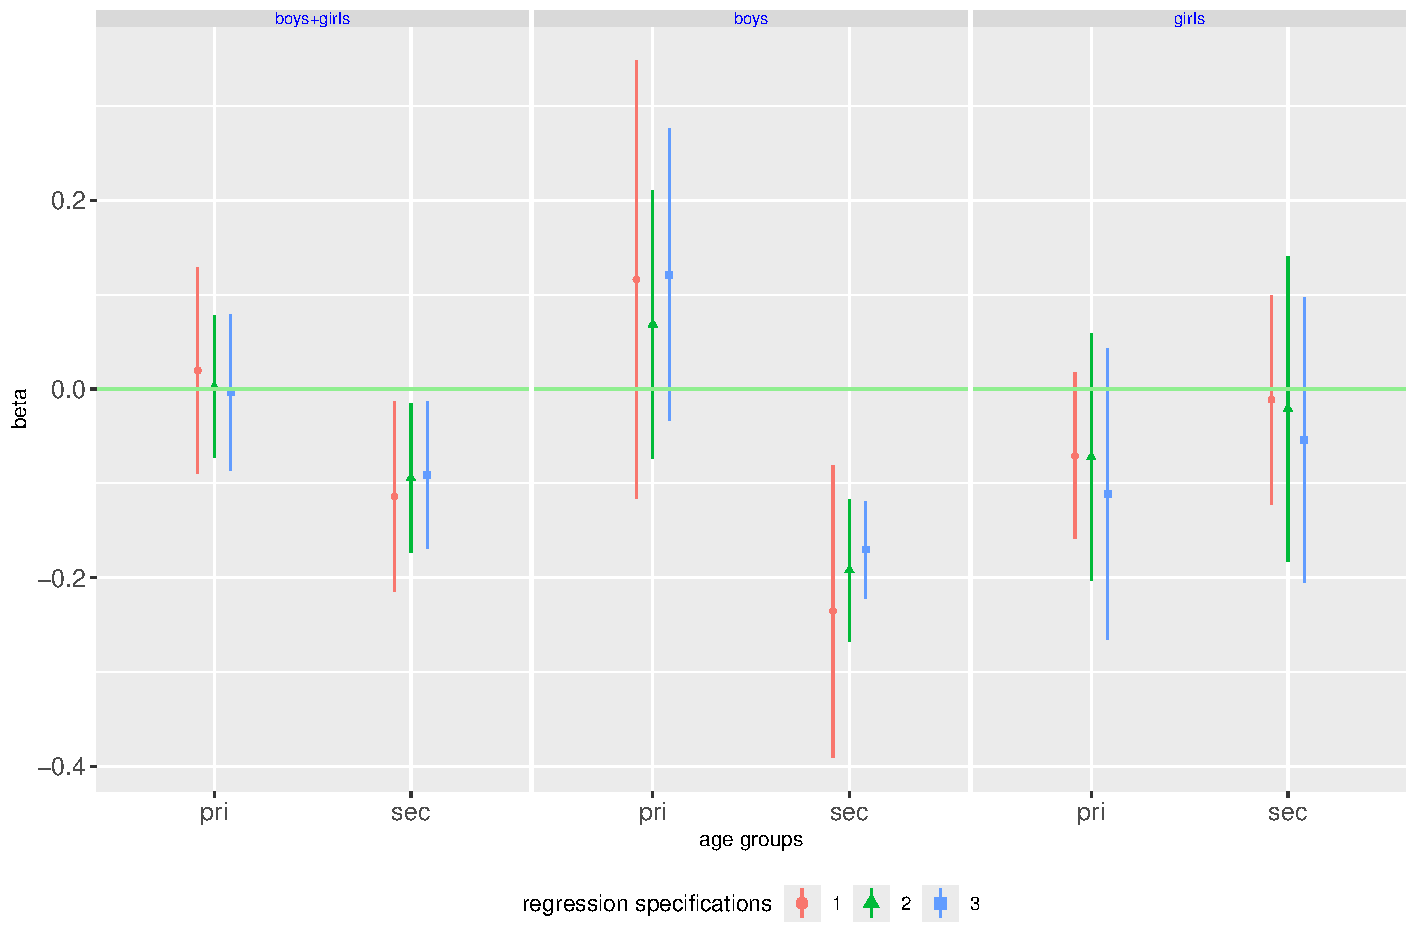
\includegraphics[height=.2\paperheight]{c:/data/ramadan/DataSubmitted/save/DIDReplication/GenderAgeGroup2Impacts.pdf}\\
\renewcommand{\arraystretch}{1}
\hfil\begin{tabular}{>{\hfill\scriptsize}p{1cm}<{}>{\scriptsize}p{12cm}<{\hfill}}
Source:& Compiled from IFPRI data. pri: 6-10, sec: 11-17  in 1999.\\[-1ex]
Notes:& 1. Coefficients on agricultural HH dummy $\times$ year 2002 dummy.'\\[-1ex]
& 2. Error bars use cluster robust standard errors at thana level with Satterthwaite correction for degree of freedom.
\end{tabular}
%\end{minipage}
\end{figure}




\begin{itemize}
\vspace{1.0ex}\setlength{\itemsep}{1.0ex}\setlength{\baselineskip}{12pt}
\item	\textsc{\footnotesize Figure \ref{ERbyAge rawdata}} shows mean enrollment rates by age. It shows ``compulsory schooling'' is not enforced strictly. 
\item	\textsc{\footnotesize Figure \ref{AgeAtClass1byAge rawdata}} shows the mean age of starting class 1. It also shows ``compulsory schooling'' is not enforced strictly. Ag HHs tend to start school later in age than nonag HHs. This may partly explain ag HH's enrollment rates are higher at some of the later ages. 
\end{itemize}




We examine other schooling outcomes available in data. Impacts on other schooling outcomes are aligned with and give certain validation to our interpretation of the main estimation results. 
\begin{itemize}
\vspace{1.0ex}\setlength{\itemsep}{1.0ex}\setlength{\baselineskip}{12pt}
\item	Number of progressed grades is fewer for ag HHs by .36 - .38 years in three years, mean annual rate of .12 - .13. This is consistent with a larger enrollment rate reduction for them.
\item	Days absent in three months prior to survey interviews show an increase in some specifications, yet the estimates are imprecise and do not statistically differ from zero. This is also consistent with the main results because days absent need not to be related to exam failures. 
\end{itemize}



{\footnotesize\bibliographystyle{aer}
\setlength{\baselineskip}{8pt}
\bibliography{c:/seiro/settings/TeX/seiro}
}

\end{document}
